\documentclass[12pt, a4paper, twoside]{book}

\usepackage[utf8]{inputenc}
\usepackage[T1]{fontenc}
\usepackage{lmodern}
\usepackage[english]{babel}
\usepackage{amsmath, amssymb, amsthm}
\usepackage{mathtools}
\usepackage{geometry}
\usepackage{graphicx}
\usepackage{hyperref}
\usepackage{enumitem}
\usepackage{booktabs}
\usepackage{array}
\usepackage{index}
\usepackage{xcolor}
\usepackage{tcolorbox}
\usepackage{tikz}
\usetikzlibrary{decorations.pathreplacing}

\geometry{margin=1in}

\hypersetup{
    colorlinks=true,
    linkcolor=blue!60!black,
    citecolor=green!50!black,
    urlcolor=blue!70!black,
}

% Theorem environments
\theoremstyle{definition}
\newtheorem{definition}{Definition}[chapter]
\newtheorem{problem_statement}{Problem Statement}[chapter]

\theoremstyle{plain}
\newtheorem{theorem}{Theorem}[chapter]
\newtheorem{lemma}[theorem]{Lemma}
\newtheorem{corollary}[theorem]{Corollary}
\newtheorem{proposition}[theorem]{Proposition}

\theoremstyle{remark}
\newtheorem{remark}[theorem]{Remark}
\newtheorem{example}[theorem]{Example}
\newtheorem{conjecture}[theorem]{Conjecture}

% Custom boxes for status
\newtcolorbox{solvedbox}{
    colback=green!5!white,
    colframe=green!60!black,
    title={Status: Solved},
    fonttitle=\bfseries
}

\newtcolorbox{partiallybox}{
    colback=yellow!5!white,
    colframe=orange!70!black,
    title={Status: Partially Solved / Ongoing},
    fonttitle=\bfseries
}

\newtcolorbox{unsolvedbox}{
    colback=red!5!white,
    colframe=red!60!black,
    title={Status: Unsolved},
    fonttitle=\bfseries
}

% Math operator shorthands
\DeclareMathOperator{\GL}{GL}
\DeclareMathOperator{\SO}{SO}
\DeclareMathOperator{\SL}{SL}
\DeclareMathOperator{\PSL}{PSL}
\DeclareMathOperator{\Gal}{Gal}
\DeclareMathOperator{\Br}{Br}
\DeclareMathOperator{\Aut}{Aut}
\DeclareMathOperator{\id}{id}
\DeclareMathOperator{\Cl}{Cl}
\DeclareMathOperator{\Gr}{Gr}
\DeclareMathOperator{\codim}{codim}
\DeclareMathOperator{\rank}{rank}
\DeclareMathOperator{\Frob}{Frob}
\DeclareMathOperator{\Diff}{Diff}

% Index
\makeindex

\title{%
    \vspace{2cm}
    {\huge\bfseries Hilbert's 23 Problems\\[0.5em]}
    {\LARGE An Independent Study Guide}
}
\author{}
\date{2026}

\begin{document}

% Cover page
\begin{titlepage}
\centering
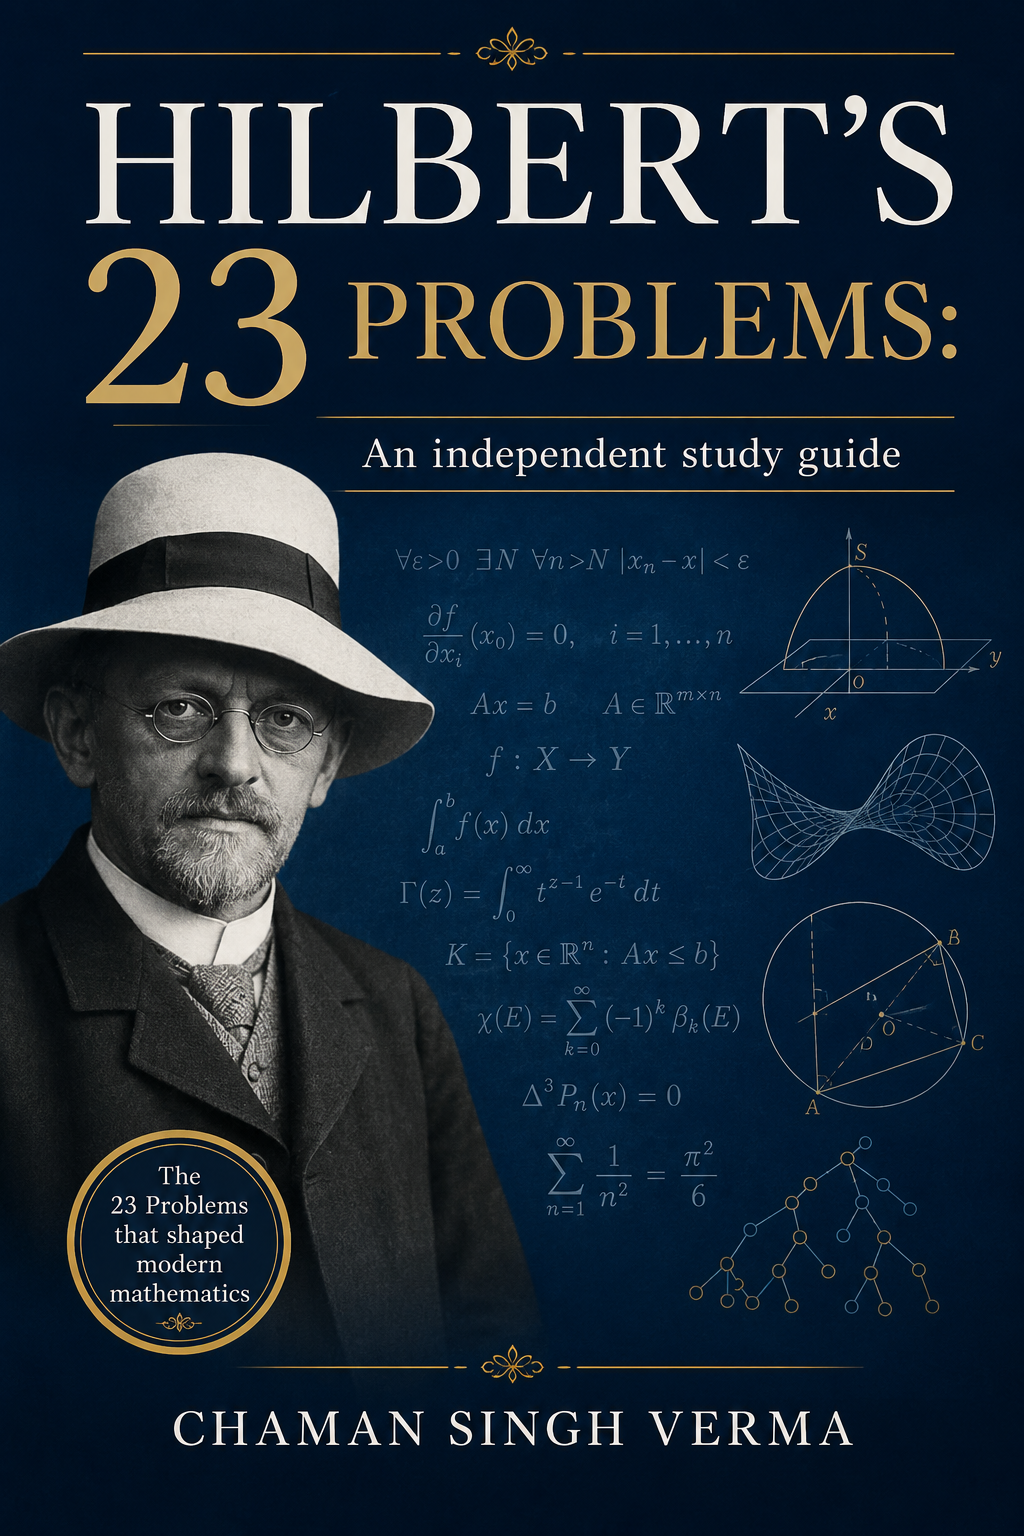
\includegraphics[width=\textwidth, height=\textheight, keepaspectratio]{frontpage.png}
\end{titlepage}

\maketitle

% ============================================================
% Front Matter: Preface, Acknowledgments, How to Use This Book
% ============================================================

\chapter*{Preface}
\addcontentsline{toc}{chapter}{Preface}

On the morning of August 8, 1900, David Hilbert stood before the assembled mathematicians of the International Congress of Mathematicians in Paris and delivered a lecture that would change the course of mathematics. In that lecture, Hilbert proposed twenty-three problems---open questions spanning the breadth of mathematics---that he believed should guide research in the coming century.

More than a century later, the legacy of that lecture endures. Hilbert's problems have served as beacons for mathematical research, inspiring entire fields and leading to some of the deepest theorems of modern mathematics. Some have been solved, some remain open, and some have evolved into questions that Hilbert could never have imagined.

This book is written for undergraduate students who wish to understand what Hilbert asked, why it mattered, and where mathematics stands today in addressing his challenges. No graduate-level background is assumed. The reader should be comfortable with calculus, basic linear algebra, and some exposure to proofs, but the mathematical details are kept at a level accessible to a motivated undergraduate.

Each chapter addresses one of Hilbert's problems. We begin with historical context---what was known in 1900 and what Hilbert hoped for. We then explain the mathematical content of the problem in modern language, describe the key ideas that led to its resolution (or progress toward it), and state the current status. Throughout, we emphasize the \emph{ideas} over technical machinery, aiming to convey the beauty and depth of these mathematical questions.

Mathematics is not a spectator sport. At the end of each chapter, you will find exercises. Some are computational, some are conceptual, and some ask you to explore further on your own. Working through them will deepen your understanding and---we hope---inspire you to learn more about the remarkable areas of mathematics that Hilbert's problems opened up.

\vspace{2em}

\noindent\textbf{Prerequisite guide by chapter.}
The book's baseline requirement is calculus, basic linear algebra, and mathematical maturity (proofs). However, the problems span the entire mathematical curriculum, and some chapters demand more. The table below maps each problem to the additional courses that will help you get the most out of that chapter.

\begin{center}
\small
\renewcommand{\arraystretch}{1.2}
\begin{tabular}{ccl}
\toprule
\textbf{Problem} & \textbf{Title} & \textbf{Recommended preparation} \\
\midrule
1 & Continuum Hypothesis & --- \\
2 & Consistency of Arithmetic & --- \\
3 & Equality of Volumes & --- \\
4 & Shortest Path = Straight Line & --- \\
5 & Continuous Groups & Linear algebra, group theory \\
6 & Axiomatization of Physics & --- \\
7 & Irrationality of $e^\pi$ & --- \\
8 & Goldbach Conjecture & --- \\
9 & Reciprocity Laws & Abstract algebra (Galois theory) \\
10 & Decision for Diophantine Eqns & --- (or computability theory) \\
11 & Quadratic Forms & Abstract algebra (rings, fields) \\
12 & Kronecker's Theorem & Abstract algebra (Galois theory) \\
13 & Solving 7th Degree Eqns & Abstract algebra (Galois theory) \\
14 & Constructive Invariants & Abstract algebra (rings, modules) \\
15 & Schubert's Enumerative Calc. & --- \\
16 & Topology of Varieties & Algebraic topology \\
17 & Representation by Squares & --- \\
18 & Tessellation of Space & --- \\
19 & Regularity of PDE Solutions & Real analysis (PDEs) \\
20 & Boundary Value Problems & Real analysis (PDEs) \\
21 & Monodromy Problem & Complex analysis \\
22 & Uniformization & Complex analysis \\
23 & Calculus of Variations & Real analysis \\
\bottomrule
\end{tabular}
\end{center}

Chapters marked ``---'' require only the baseline. Each chapter defines its own concepts, so you can always \emph{read} a chapter above your preparation; starred exercises ($\star$) in advanced chapters will be harder without the listed background. The book is designed to be read non-linearly---skip around freely.

\chapter*{Acknowledgments}

\chapter*{Acknowledgments}
\addcontentsline{toc}{chapter}{Acknowledgments}

This book draws on over a century of mathematical scholarship. We are indebted to the many mathematicians who solved, advanced, and illuminated Hilbert's problems. Particular gratitude is due to Jeremy Gray, whose historical scholarship on Hilbert's problems has been invaluable; to Constance Reid, whose biography of Hilbert remains the definitive account; and to the many mathematicians who have written expositions of individual problems, making them accessible to broader audiences.

We also thank the generations of students whose questions and curiosity helped shape this exposition. Any errors that remain are, of course, our own.

\chapter*{How to Use This Book}
\addcontentsline{toc}{chapter}{How to Use This Book}

\begin{itemize}
    \item \textbf{Each chapter} addresses one of Hilbert's 23 problems and is self-contained. You may read them in order or jump to problems that interest you.

    \item \textbf{Historical context} appears at the beginning of each chapter, explaining what was known in 1900.

    \item \textbf{The problem} is stated in modern mathematical language, as close to Hilbert's original intent as possible.

    \item \textbf{Key developments} describe the major results and ideas that have addressed the problem.

    \item \textbf{Current status} summarizes where the problem stands today, using the following conventions:
    \begin{itemize}
        \item \textbf{Solved:} A complete answer (or proof of impossibility) is known.
        \item \textbf{Partially solved:} Significant progress has been made, but the full problem remains open.
        \item \textbf{Unsolved:} Little progress, or the problem remains wide open.
        \item \textbf{Independent:} The problem cannot be decided within standard axiom systems (a different kind of resolution).
    \end{itemize}

    \item \textbf{Exercises} range from routine to challenging. star-marked exercises ($\star$) are more difficult.

    \item \textbf{Appendices} provide a timeline, glossary of terms, and suggestions for further reading.
\end{itemize}


\tableofcontents

\mainmatter

% ============================================================
% Chapter 1: Introduction — Hilbert and His 23 Problems
% ============================================================

\chapter*{David Hilbert and His 23 Problems}
\addcontentsline{toc}{chapter}{Introduction: David Hilbert and His 23 Problems}

\section{The Man Behind the Problems}

David Hilbert (1862--1943) was born in K\"onigsberg, Prussia (now Kaliningrad, Russia), a city with a storied mathematical heritage---it was where Carl Jacobi had taught and where the young Hilbert would walk and talk mathematics with his friend Hermann Minkowski and their teacher Ferdinand von Lindemann.

Hilbert's early work was in invariant theory, where he proved a finite basis theorem that stunned the mathematical world. When Paul Gordan, the self-styled ``king of invariants,'' saw Hilbert's proof---a short, elegant argument where pages of computation had been the norm---he reportedly said: ``Das ist nicht Mathematik. Das ist Theologie.'' (``This is not mathematics. This is theology.'') But the proof was correct, and it opened a new way of thinking about existence proofs.

By 1900, Hilbert was already a prominent figure in G\"ottingen, one of the great mathematical centers of the world. He had moved from invariant theory to number theory, algebraic geometry, and the foundations of mathematics. He was a man of enormous vision, capable of seeing the deep connections between seemingly disparate areas of mathematics.

\section{The Second International Congress of Mathematicians}

The International Congress of Mathematicians (ICM) met in Paris in August 1900, timed to coincide with the opening of the Paris World's Fair. The Congress was a grand affair---a celebration of mathematics at the dawn of a new century. Henri Poincar\'e, the greatest mathematician of the age, delivered the opening address.

Hilbert was invited to give a lecture. His choice of topic was remarkable. Rather than presenting his own research, Hilbert decided to look forward. He would propose problems that should occupy mathematicians in the coming century.

\begin{quote}
\textit{``Who among us would not like to lift the veil behind which the future lies hidden and cast a glance at the coming advances of our science and the secrets of its development during future centuries? What new goals and what new methods will the new century reveal to us in the field of mathematics, whose old flora has been gathered so richly by the heroic exertions of previous centuries?''}
\par\hfill ---David Hilbert, 1900
\end{quote}

On the morning of August 8, 1900, Hilbert presented his list. It was not a complete list---he did not claim to have found all the important problems. ``Rather will it be the task of the future to follow the tracks he has blazed,'' he said of the problems of the past. ``Guided by the clear signs which they have left behind them, we may hope to gain a view of the whole of the yet unexplored domain of the mathematical sciences, and thus of the means whereby we may attack the problems which it contains.''

He then outlined twenty-three problems, spanning number theory, algebra, geometry, analysis, mathematical physics, and the foundations of mathematics. The problems were not chosen at random. They were carefully selected---each one was, in Hilbert's view, a doorway into a deep and important area of mathematics.

\section{The Problems: An Overview}

The twenty-three problems can be grouped into several broad areas:

\begin{enumerate}
    \item \textbf{Number Theory and Algebra} (Problems 1, 8, 9, 10, 11, 12, 13, 14): Questions about prime numbers, Diophantine equations, algebraic number fields, and the solvability of equations by radicals.

    \item \textbf{Geometry} (Problems 3, 4, 5, 6, 16, 18): Questions about volume, the concept of distance, continuous groups, the axioms of geometry, and tessellations of space.

    \item \textbf{Analysis} (Problems 2, 15, 17, 19, 20, 21, 22, 23): Questions about the continuum, calculus of variations, boundary value problems, and the monodromy theorem.

    \item \textbf{Mathematical Physics} (Problems 6, 19): The relationship between physics and mathematics, and the problem of regularity of solutions to equations of mathematical physics.

    \item \textbf{Logic and Foundations} (Problems 2, 7): The consistency of arithmetic and the nature of irrational numbers.
\end{enumerate}

The following table gives a bird's-eye view of all 23 problems and their current status:

\begin{center}
\small
\renewcommand{\arraystretch}{1.2}
\begin{tabular}{clll}
\toprule
\textbf{\#} & \textbf{Problem (short title)} & \textbf{Year Solved} & \textbf{Status} \\
\midrule
1 & Continuum Hypothesis & 1963 & Independent \\
2 & Consistency of Arithmetic & 1931 & Resolved \\
3 & Equality of Volumes (Tetrahedra) & 1901 & Solved \\
4 & Shortest Path = Straight Line & 1900s & Solved \\
5 & Continuous Groups = Manifolds & 1920s & Solved \\
6 & Axioms of Physics & --- & Partially Solved \\
7 & Irrationality of $e^\pi$ & 1934 & Solved \\
8 & Goldbach Conjecture & --- & Unsolved \\
9 & Reciprocity Laws & 1920s & Solved \\
10 & Decision for Diophantine Equations & 1970 & Solved \\
11 & Quadratic Forms & 1930s & Partially Solved \\
12 & Kronecker's Theorem & 1920s & Solved \\
13 & Solving 7th Degree by Radicals & 1900s & Solved \\
14 & Constructive Algebraic Invariants & 1950s & Partially Solved \\
15 & Schubert's Enumerative Calculus & --- & Partially Solved \\
16 & Topology of Algebraic Curves & --- & Partially Solved \\
17 & Representation by Quadratic Forms & 1920s & Solved \\
18 & Tessellation of Space & 1910--11 & Solved \\
19 & Regularity of PDE Solutions & 1904--57 & Partially Solved \\
20 & Boundary Value Problems & --- & Partially Solved \\
21 & Monodromy Problem & 1950s & Solved \\
22 & Uniformization & 1907--13 & Solved \\
23 & Calculus of Variations & 1900s+ & Partially Solved \\
\bottomrule
\end{tabular}
\end{center}

\section{Why These Problems Matter}

Hilbert's problems are not just historical artifacts. They remain central to modern mathematics. Several of the deepest results of 20th-century mathematics---G\"odel's incompleteness theorems, the proof of the Weil conjectures, the resolution of the Poincar\'e conjecture (not one of Hilbert's, but related in spirit), the classification of finite simple groups---were motivated directly or indirectly by Hilbert's vision.

More importantly, the problems illustrate what mathematics \emph{is}: a living, evolving discipline where the deepest questions of one generation become the foundational theorems of the next.

\section{A Guide for the Reader}

This book proceeds as follows. Each of the next 23 chapters addresses one of Hilbert's problems. The chapters are written to be self-contained---you may read them in any order. Each chapter includes:

\begin{itemize}
    \item \textbf{Historical Context}: What was known in 1900 and why the problem mattered.
    \item \textbf{The Problem}: Stated in modern mathematical language.
    \item \textbf{Key Developments}: The major ideas and results that addressed the problem.
    \item \textbf{Current Status}: Where the problem stands today.
    \item \textbf{Exercises}: Problems to test your understanding.
\end{itemize}

No single book can teach all the mathematics needed to fully appreciate every one of Hilbert's problems. But we can convey the essential ideas, and we can inspire the reader to seek out more.

\section*{Exercises}

\begin{enumerate}
    \item Research and write a one-page biography of David Hilbert. What were his major contributions to mathematics beyond the 23 problems?

    \item Hilbert said, ``Wir m\"ussen wissen. Wir werden wissen.'' (``We must know. We will know.'') What did he mean, and how does this relate to the problems he proposed?

    \item Choose three of the 23 problems that you find interesting after reading the table above. For each, write one sentence explaining why you chose it.
\end{enumerate}


% The 23 Problems
\setcounter{chapter}{0}
% ============================================================
% Chapter 2: Hilbert's Problem 1 — The Continuum Hypothesis
% ============================================================

\chapter{The Continuum Hypothesis}

\begin{unsolvedbox}
\textbf{Note:} This problem is not ``unsolved'' in the traditional sense. It has been \emph{resolved}---but in a way that Hilbert could not have anticipated. The Continuum Hypothesis is \textbf{independent} of the standard axioms of set theory (ZFC): it can be neither proved nor disproved from those axioms. This is a fundamentally different kind of answer than a proof or disproof, and it raises profound questions about the nature of mathematical truth.
\end{unsolvedbox}

% ------------------------------------------------------------
\section{Historical Context}
% ------------------------------------------------------------

In the closing decades of the nineteenth century, Georg Cantor (1845--1918) created something entirely new: a rigorous theory of \emph{infinite sets}. Before Cantor, infinity was treated with suspicion---a vague philosophical notion rather than a mathematical object. Cantor changed that. He showed that infinite sets can be compared in size, that some infinities are strictly larger than others, and that this comparison obeys precise mathematical laws.

The key idea is \textbf{cardinality}. Two sets $A$ and $B$ have the same cardinality if there exists a bijection $f\colon A \to B$. If such a bijection exists, we say $|A| = |B|$. If every function from $A$ to $B$ fails to be surjective (onto), we say $|A| < |B|$.

Cantor proved in 1874 that the natural numbers $\mathbb{N} = \{0, 1, 2, 3, \ldots\}$ and the real numbers $\mathbb{R}$ do \emph{not} have the same cardinality. His original proof used a clever argument about bounded monotone sequences, but the argument he published in 1891---his famous \emph{diagonal argument}---is the one that has endured.

\begin{theorem}[Cantor's Diagonal Argument, 1891]
\label{thm:diagonal}
The set of real numbers in the interval $(0,1)$ is uncountable. That is, there is no surjection from $\mathbb{N}$ onto $(0,1)$.
\end{theorem}

\begin{proof}
Suppose for contradiction that $f \colon \mathbb{N} \to (0,1)$ is surjective. Write each $f(n)$ in its decimal expansion:
\[
    f(n) = 0.d_{n1}\, d_{n2}\, d_{n3}\, \cdots
\]
where each $d_{nk} \in \{0, 1, \ldots, 9\}$. (To avoid ambiguity, we never use an expansion ending in all $9$s.)

Define a new real number $r = 0.r_1 r_2 r_3 \cdots$ by choosing
\[
    r_n = \begin{cases} 3 & \text{if } d_{nn} \neq 3, \\ 7 & \text{if } d_{nn} = 3. \end{cases}
\]
Then $r \in (0,1)$ but $r \neq f(n)$ for every $n \in \mathbb{N}$, since $r$ differs from $f(n)$ in the $n$th decimal place. This contradicts the assumption that $f$ is surjective.
\end{proof}

This result established that $|\mathbb{N}| < |\mathbb{R}|$. Cantor introduced notation for these cardinalities. The cardinality of $\mathbb{N}$ is called \textbf{countable infinity} and denoted $\aleph_0$ (read ``aleph-null''). The cardinality of $\mathbb{R}$ is called the \textbf{continuum} and denoted $\mathfrak{c}$.

So Cantor knew that $\aleph_0 < \mathfrak{c}$. The natural question was: is there anything \emph{in between}? That is, does there exist a set $S$ with
\[
    \aleph_0 < |S| < \mathfrak{c} \, ?
\]
This question is the Continuum Hypothesis.

By 1900, Cantor had spent years trying to prove that no such set exists---that is, that $\mathfrak{c} = \aleph_1$, where $\aleph_1$ is the next cardinal after $\aleph_0$. He exchanged letters with Dedekind on the topic and wrote passionately about it, but he never found a proof. The question was wide open when Hilbert placed it first on his list of twenty-three problems.

% ------------------------------------------------------------
\section{The Problem}
% ------------------------------------------------------------

\begin{problem_statement}[The Continuum Hypothesis]
There is no set whose cardinality is strictly between that of the integers and that of the real numbers. Equivalently:
\[
    \mathfrak{c} = \aleph_1.
\]
\end{problem_statement}

Let us unpack this statement.

\subsection{Aleph Numbers and the Well-Ordering Principle}

Cantor showed that the class of infinite cardinal numbers is itself well-ordered by $<$: given any set of cardinal numbers, there is a smallest one. This means we can list the infinite cardinals in a sequence indexed by the ordinal numbers:
\[
    \aleph_0,\ \aleph_1,\ \aleph_2,\ \aleph_3,\ \ldots,\ \aleph_\omega,\ \aleph_{\omega+1},\ \ldots
\]
Here $\aleph_0$ is the cardinality of $\mathbb{N}$, $\aleph_1$ is the smallest uncountable cardinal, $\aleph_2$ is the next one, and so on. The aleph numbers are the infinite cardinals \emph{in canonical order}.

The real number continuum has cardinality $\mathfrak{c} = 2^{\aleph_0}$, by Cantor's theorem that the power set of any set $X$ has strictly greater cardinality than $X$ itself. The Continuum Hypothesis is the assertion that
\[
    2^{\aleph_0} = \aleph_1.
\]
More generally, the \textbf{Generalized Continuum Hypothesis} (GCH) asserts that for every ordinal $\alpha$,
\[
    2^{\aleph_\alpha} = \aleph_{\alpha+1}.
\]

\subsection{Why It Matters}

The Continuum Hypothesis asks about the most basic structure of the infinite: the ``size'' of the real number line. If CH is true, then the real line is as ``thin'' as it could possibly be---there are no infinite sets squeezed between $\mathbb{N}$ and $\mathbb{R}$ in size. If CH is false, then the landscape of infinity is richer and more complicated than that, with one or more infinite cardinalities lying strictly between countable and continuum.

This question touches the foundations of nearly all of mathematics. Real analysis, topology, measure theory, and the theory of function spaces all depend on the structure of $\mathbb{R}$ and its subsets. If the cardinality of $\mathbb{R}$ has unexpected properties, the consequences ripple outward.

% ------------------------------------------------------------
\section{Key Developments}
% ------------------------------------------------------------

The story of the Continuum Hypothesis is one of the great intellectual dramas of the twentieth century. It unfolds in three acts.

\subsection{The Search for a Proof (1900--1940)}

Hilbert placed CH first on his list because he believed it should be provable---that a clever argument would eventually show $\mathfrak{c} = \aleph_1$. For decades, set theorists tried. The problem attracted some of the best minds in mathematical logic, but progress was elusive.

Cantor himself died in 1918, having never resolved the question. The tools of the time were simply not powerful enough to settle it.

\subsection{G\"odel's Constructible Universe (1940)}

In 1931, Kurt G\"odel (1906--1978) had already shocked the mathematical world with his \emph{incompleteness theorems}, which showed that any consistent formal system powerful enough to describe arithmetic contains true statements that cannot be proved within the system. This raised a natural question: could the Continuum Hypothesis be one of those undecidable statements?

G\"odel made dramatic progress in 1940. He introduced a remarkable construction called the \textbf{constructible universe}, denoted $L$.

The idea is as follows. Start with the empty set and build upward, at each stage adding only those sets that are ``definable'' in a precise sense. More formally, define a hierarchy of sets $L_\alpha$, indexed by ordinal numbers $\alpha$:
\begin{itemize}
    \item $L_0 = \varnothing$,
    \item $L_{\alpha+1} = \mathrm{Def}(L_\alpha)$, the collection of all subsets of $L_\alpha$ that are definable over $(L_\alpha, \in)$ using first-order formulas with parameters from $L_\alpha$,
    \item $L_\lambda = \bigcup_{\alpha < \lambda} L_\alpha$ for limit ordinals $\lambda$.
\end{itemize}
The constructible universe is $L = \bigcup_{\alpha \in \mathrm{Ord}} L_\alpha$.

G\"odel proved two crucial theorems:

\begin{theorem}[G\"odel, 1940]
\label{thm:goedel-ch}
If ZFC is consistent, then ZFC $+$ CH is consistent.
\end{theorem}

The proof strategy is: assuming ZFC is consistent, the constructible universe $L$ is a model of ZFC in which CH holds. In $L$, the continuum hypothesis is true. Therefore, no contradiction can be derived from ZFC $+$ CH (assuming ZFC itself is consistent).

This was a landmark result. It showed that CH \emph{cannot be disproved} from the axioms of set theory (assuming those axioms are consistent). But it left open the question: could CH be \emph{proved}?

\subsection{Cohen's Forcing (1963)}

The answer came in 1963, when Paul Cohen (1928--2007) introduced a revolutionary new technique called \textbf{forcing}.

Cohen's method works in the opposite direction from G\"odel's. Instead of building an inner model where CH holds, forcing constructs a \emph{generic extension} of a model of ZFC in which CH fails.

The intuition behind forcing is as follows. Start with a model $M$ of ZFC. One wants to add a new ``generic'' set $G$ to $M$ in such a way that the enlarged universe $M[G]$ still satisfies all the axioms of ZFC, but $G$ has properties that $M$ did not satisfy. The generic set is designed to ``encode'' enough subsets of $\omega$ (and hence of $\mathbb{R}$) to make $2^{\aleph_0}$ strictly larger than $\aleph_1$.

Cohen proved:

\begin{theorem}[Cohen, 1963]
\label{thm:cohen-nch}
If ZFC is consistent, then ZFC $+$ $\neg$CH is consistent.
\end{theorem}

The technical details of forcing are demanding, but the essential idea is a sophisticated version of a simple principle: if you cannot prove a statement, you can sometimes construct a mathematical universe in which it is false, without creating any contradictions.

\subsection{Putting It Together}

Combining G\"odel's and Cohen's results gives a remarkable conclusion:

\begin{theorem}
If ZFC is consistent, then CH is \textbf{independent} of ZFC. That is, ZFC $\not\vdash$ CH and ZFC $\not\vdash$ $\neg$CH.
\end{theorem}

This means that the Continuum Hypothesis can be neither proved nor disproved from the standard axioms of set theory. It is ``undecidable'' in ZFC.

% ------------------------------------------------------------
\section{Current Status: Independent of ZFC}
% ------------------------------------------------------------

The resolution of the Continuum Hypothesis is one of the most profound results in the foundations of mathematics. But it raises as many questions as it answers.

\subsection{What Does Independence Mean?}

Independence means that the axioms of ZFC simply do not determine the truth value of CH. Both the universe where CH holds and the universe where CH fails are perfectly legitimate models of ZFC. There is no ``mistake'' in either case.

This is sometimes unsettling to students who expect mathematics to provide definite answers. But independence is itself a precise mathematical fact, proved by the methods of mathematical logic. The answer to Hilbert's first problem is: \emph{the question as stated cannot be resolved within the standard framework}.

\subsection{Beyond ZFC: New Axioms}

Many set theorists believe that ZFC is not the final word---that there are natural additional axioms that \emph{should} be accepted, and that might settle CH.

\paragraph{Martin's Axiom (MA).}
Martin's Axiom is a ``weak'' generalization of the Continuum Hypothesis. Formally, MA asserts that for every $\sigma$-closed partial order $\mathbb{P}$ and every collection of fewer than $2^{\aleph_0}$ dense subsets of $\mathbb{P}$, there is a filter meeting all of them. Martin's Axiom is consistent with both CH and $\neg$CH, but in combination with $\neg$CH it has powerful consequences. For instance, ZFC $+$ MA $+$ $2^{\aleph_0} = \aleph_2$ implies that the union of fewer than $2^{\aleph_0}$ measure-zero sets has measure zero, and that the union of fewer than $2^{\aleph_0}$ meager sets is meager. MA is widely regarded as a ``natural'' principle that enriches ZFC without leading to pathology.

\paragraph{Large Cardinal Axioms.}
The most active direction in contemporary set theory involves \textbf{large cardinal axioms}---axioms asserting the existence of very large infinite cardinals with special properties (inaccessible cardinals, measurable cardinals, Woodin cardinals, supercompact cardinals, etc.). These axioms are arranged in a linear hierarchy of consistency strength, and they have far-reaching consequences for the structure of the set-theoretic universe.

Hugh Woodin (b.\ 1955) has argued that large cardinal axioms, particularly the existence of \textbf{Woodin cardinals}, provide evidence that $\neg$CH is the ``correct'' answer. His work, building on results of Donald Martin and John Steel, shows that certain large cardinal assumptions imply that the theory of $L(\mathbb{R})$ (the constructible universe built over the reals) is determined and canonical.

\paragraph{Woodin's $\ast$-Axiom.}
Woodin introduced an axiom---often denoted $\ast$---that implies $\neg$CH and, together with large cardinal axioms, determines the theory of $H(\omega_2)$ (the collection of sets hereditarily of cardinality less than $\aleph_2$). This axiom has been the subject of intense study and debate. Whether it should be ``accepted'' as a new axiom of set theory is an open philosophical question.

\subsection{The Role of CH in Modern Set Theory}

Despite---or perhaps because of---its independence, CH remains one of the central organizing questions of set theory. The search for new axioms that might settle CH has driven some of the deepest research in the field. Cohen's method of forcing has become one of the most important tools in all of set theory, with applications far beyond the original question.

The problem also raised foundational issues that continue to resonate. If the axioms of set theory do not determine the value of $2^{\aleph_0}$, what does that say about mathematical objects like the real line? Are the reals ``definite'' in the way we thought? These questions connect Hilbert's first problem to the deepest issues in the philosophy of mathematics.

In a sense, Hilbert's first problem was ``resolved''---but the resolution was so unexpected and so rich that it opened up entirely new areas of mathematics. This is perhaps the highest compliment one can pay to a mathematical problem.

% ------------------------------------------------------------
\section{Summary}
% ------------------------------------------------------------

\begin{center}
\renewcommand{\arraystretch}{1.3}
\begin{tabular}{ll}
\toprule
\textbf{Aspect} & \textbf{Details} \\
\midrule
Problem & Is $\mathfrak{c} = \aleph_1$? (Continuum Hypothesis) \\
Proposed by & Georg Cantor (1874--1891); placed first on Hilbert's list \\
Key result I & G\"odel (1940): CH is consistent with ZFC (via $L$) \\
Key result II & Cohen (1963): $\neg$CH is consistent with ZFC (via forcing) \\
Current status & \textbf{Independent of ZFC} (undecidable in standard axioms) \\
Ongoing work & Large cardinals, Martin's Axiom, Woodin's $\ast$-axiom \\
\bottomrule
\end{tabular}
\end{center}

% ------------------------------------------------------------
\section*{Common Questions}
% ------------------------------------------------------------

\begin{description}[font=\bfseries, leftmargin=2em, style=nextline]

\item[Q: What does it mean for CH to be ``independent'' of ZFC? Is it solved or not?]\hfill\\
It means CH can neither be proved nor disproved from the ZFC axioms (assuming ZFC is consistent). It is ``solved'' in the sense that we know the answer is ``it depends on your axioms''---but not in the sense that we know whether the continuum's actual cardinality is $\aleph_1$. Independence is a meta-mathematical fact about what ZFC can prove, not a direct answer about sets.

\item[Q: Can we just add CH as a new axiom and move on?]\hfill\\
We can, and some mathematicians have argued for doing exactly that. The problem is that adding CH settles some questions but leaves others open, and it rules out interesting mathematics that requires $\neg$CH (e.g., certain consequences of Martin's Axiom). Moreover, adding an axiom just because we like its conclusion is philosophically questionable---we want axioms that are ``obvious'' or ``intrinsic,'' and CH is neither.

\item[Q: Does forcing actually construct a new mathematical universe?]\hfill\\
In a precise technical sense, yes. Forcing starts with a model $V$ of ZFC and extends it to a larger model $V[G]$ that contains a ``generic'' object $G$ not in $V$. The result is a new model of set theory that satisfies ZFC~$+~\neg$CH (or ZFC~$+$~CH, depending on the forcing). Whether you think these are ``real'' mathematical universes or just syntactic constructs depends on your philosophical views.

\item[Q: Why does Hilbert call this Problem~1 if it's about set theory, not arithmetic?]\hfill\\
Hilbert's list was not ordered by subject but by importance and interconnectedness. CH was first because Cantor's continuum problem was the most famous unsolved question in the foundation of mathematics---the very foundation on which all of arithmetic, analysis, and geometry rest. Hilbert believed the problem would yield to arithmetic methods, which turned out to be wrong, but the problem's centrality was never in doubt.

\item[Q: I've heard that CH being independent means math is ``broken.'' Is that true?]\hfill\\
Not at all. Independence is a feature of the mathematical landscape, not a bug. Many important statements are independent of weaker axiom systems (e.g., the Parallel Postulate is independent of Euclid's other axioms). The independence of CH from ZFC tells us that ZFC does not fully determine the nature of the continuum---which is a deep and interesting fact about set theory, not a sign that something is wrong.

\item[Q: What exactly is $\aleph_1$, and how is it different from the cardinality of $\mathbb{R}$?]\hfill\\
$\aleph_1$ is the first uncountable cardinal---the cardinality of the set of all countable ordinals. It is, by definition, the smallest cardinal greater than $\aleph_0$ (the cardinality of $\mathbb{N}$). The cardinality of $\mathbb{R}$ is $2^{\aleph_0} = \mathfrak{c}$ (the continuum). CH says these are equal: $\mathfrak{c} = \aleph_1$. If CH fails, $\mathfrak{c}$ is larger than $\aleph_1$---possibly $\aleph_2$ or even bigger.

\item[Q: Do large cardinal axioms decide CH?]\hfill\\
No. Standard large cardinal axioms (measurable, strong, Woodin, supercompact) are all consistent with both CH and $\neg$CH. This is one of the most striking facts about independence: even very strong axioms do not settle the size of the continuum. Woodin's $\Omega$-conjecture and the search for a ``canonical'' model of set theory that might settle CH is one of the most active areas of research. See Chapter~21 for more on large cardinals.

\end{description}

% ------------------------------------------------------------
\section*{Exercises}
% ------------------------------------------------------------

\begin{enumerate}

    \item \textbf{Cantor's Diagonal Argument.}
    \begin{enumerate}
        \item Adapt the proof of Theorem~\ref{thm:diagonal} to show directly that there is no surjection from $\mathbb{N}$ onto $\{0,1\}^{\mathbb{N}}$ (the set of all infinite binary sequences).
        \item Use the fact that $\{0,1\}^{\mathbb{N}}$ has the same cardinality as $\mathcal{P}(\mathbb{N})$ (the power set of $\mathbb{N}$) to conclude that $|\mathcal{P}(\mathbb{N})| > |\mathbb{N}|$. This is a special case of Cantor's theorem.
    \end{enumerate}

    \item \textbf{Cardinality of the Reals.}
    Using Cantor's theorem that $|X| < |\mathcal{P}(X)|$ for any set $X$, prove that $|\mathbb{R}| = 2^{\aleph_0}$. (\emph{Hint:} Construct an injection from $\mathcal{P}(\mathbb{N})$ to $\mathbb{R}$ using binary expansions, and an injection from $\mathbb{R}$ to $\mathcal{P}(\mathbb{Q})$ using open intervals with rational endpoints.)

    \item \textbf{The Generalized Continuum Hypothesis.}
    \begin{enumerate}
        \item State the Generalized Continuum Hypothesis (GCH) precisely.
        \item Show that GCH implies CH.
        \item Is the converse true? (That is, does CH imply GCH?)
    \end{enumerate}

    \item \textbf{Independence and Models.}
    \begin{enumerate}
        \item Explain in your own words what it means for a statement $\varphi$ to be \emph{independent} of a set of axioms $\Sigma$.
        \item What would it mean for a statement to be independent of ZFC? Does this mean the statement is ``meaningless'' or ``true in some sense and false in another''? Discuss in one or two paragraphs.
    \end{enumerate}

    \item[$\star$] \textbf{Cohen's Forcing: A Toy Example.}
    The full details of forcing are beyond this chapter, but here is a toy illustration of the core idea. Consider the partial order $\mathbb{P}$ consisting of all \emph{finite} partial functions $p \colon \omega \to \{0,1\}$, ordered by reverse inclusion ($p \leq q$ iff $p \supseteq q$). A filter $G$ on $\mathbb{P}$ that meets every dense subset of $\mathbb{P}$ corresponds to a \emph{generic} function $g \colon \omega \to \{0,1\}$, which can be viewed as a subset of $\omega$. Explain informally why a ``generic'' such $g$ should be expected to encode a subset of $\omega$ that is \emph{not} in the ground model. Why does this suggest that one can force the continuum to be large?

\end{enumerate}

% ============================================================
% Chapter 3: Hilbert's Problem 2 — The Consistency of Arithmetic
% ============================================================

\chapter{The Consistency of the Axioms of Arithmetic}

\begin{solvedbox}
\textbf{Resolved (1931).} G\"odel's second incompleteness theorem showed that no sufficiently strong, consistent formal system can prove its own consistency---precisely the kind of internal proof Hilbert had hoped for. The problem is solved, but in a negative sense: Hilbert's original goal turned out to be unachievable.
\end{solvedbox}

% -----------------------------------------------------------
\section{Historical Context: The Foundational Crisis}
% -----------------------------------------------------------

By the end of the nineteenth century, mathematics faced a crisis of confidence. The subject had grown substantially in scope and power, but no one could say with certainty that its foundations were secure.

\subsection{The Dream of Rigor}

Since the time of Euclid, mathematicians had organized their knowledge into systems of \emph{axioms}---self-evident truths from which all theorems follow by logical deduction. Geometry had been axiomatized with great precision by Hilbert himself in his \emph{Grundlagen der Geometrie} (1899). But arithmetic---the simplest and most fundamental branch of mathematics---had never received the same treatment.

What would a complete, rigorous axiomatization of arithmetic look like? Two efforts in particular set the stage.

\subsection{Frege's Logicism}

In 1879, the German logician and philosopher Gottlob Frege published his \emph{Begriffsschrift} (``Concept Script''), a revolutionary system of formal logic. Frege's dream was \emph{logicism}: the idea that all of mathematics could be reduced to pure logic. If successful, this would ground arithmetic---and all of mathematics---in the bedrock of logical reasoning.

Over the next two decades, Frege developed an elaborate logical system. His \emph{Grundgesetze der Arithmetik} (``Basic Laws of Arithmetic'') aimed to derive the natural numbers and their properties from purely logical axioms. Then, in 1901, disaster struck. Bertrand Russell wrote to Frege with a devastating observation:

\begin{quote}
\textit{``Let $R$ be the relation of belonging to the class under consideration. Does the class of all classes that do not belong to themselves belong to itself?''}
\end{quote}

This is the now-famous \textbf{Russell's Paradox}. If such a class exists, it belongs to itself if and only if it does not belong to itself---a contradiction. Russell's paradox showed that Frege's system was inconsistent. Frege himself, upon receiving the letter, wrote: ``A scientist can hardly encounter anything more undesirable than to have the foundation collapse just as the work is finished.''

\subsection{The Peano Axioms}

Independently of Frege, Giuseppe Peano had published in 1889 a set of axioms for the natural numbers, stated in a notation that used logical symbols but did not aim for full logical reduction. The Peano axioms remain the standard starting point for the formal theory of arithmetic:

\begin{enumerate}[label=\textbf{P\arabic*}, leftmargin=2em]
    \item $0$ is a natural number.
    \item For every natural number $n$, $S(n)$ (the \emph{successor} of $n$) is a natural number.
    \item There is no natural number whose successor is $0$.
    \item If $S(m) = S(n)$, then $m = n$.
    \item \emph{The Axiom of Induction:} If $\varphi$ is a property such that $\varphi(0)$ holds, and for every $n$, $\varphi(n)$ implies $\varphi(S(n))$, then $\varphi(n)$ holds for all natural numbers $n$.
\end{enumerate}

These five axioms generate all of arithmetic. Addition and multiplication are defined recursively, and all the familiar properties of arithmetic---commutativity, associativity, the distributive law---are proved from the axioms by induction.

But here is the crucial question: \emph{are these axioms consistent?} Can we be sure that no contradiction follows from them?

\subsection{The Desire for an Internal Proof}

This question was not merely philosophical. If Peano's axioms are inconsistent, then \emph{every} statement is provable from them---including false ones. The entire edifice of number theory would collapse.

Hilbert recognized that the axioms of geometry had been proved consistent relative to the axioms of arithmetic (via coordinate geometry). But this merely pushed the question one level deeper: what certifies the consistency of arithmetic itself?

Hilbert's answer---his \emph{finitist program}---was bold. He proposed that the consistency of arithmetic should be proved by \emph{finitary methods}: simple, concrete, combinatorial reasoning about finite strings of symbols, methods so elementary that their reliability could not be in doubt. Such a proof would be an \emph{internal} proof---a proof conducted entirely within methods more basic than those whose consistency was in question.

\begin{quote}
\textit{``To prove the consistency of arithmetic, we must use only such methods as we are certain are reliable. These finitary methods are so concrete and simple that their correctness can be recognized a priori.''}\par\hfill ---David Hilbert, paraphrased
\end{quote}

This was the heart of Problem 2.

% -----------------------------------------------------------
\section{The Problem}
% -----------------------------------------------------------

In his 1900 lecture, Hilbert stated the second problem as follows:

\begin{problem_statement}
Prove that the axioms of arithmetic are consistent---that is, free from contradiction---by methods that are themselves beyond doubt.
\end{problem_statement}

More precisely, Hilbert asked for a proof of the consistency of the natural numbers that uses only \emph{finitary} means. What counts as ``finitary'' was left somewhat open, but Hilbert had in mind reasoning about finite sequences of symbols, elementary combinatorial arguments, and direct verification of specific configurations---methods that involve no appeal to completed infinities or non-constructive principles.

The idea was to establish a hierarchy of certainty:
\begin{enumerate}
    \item \emph{Finitary} reasoning: the most basic and secure.
    \item \emph{Infinitary} methods (involving quantifiers over infinite sets, induction over arbitrary properties): powerful but less secure.
    \item \emph{Set-theoretic} methods (involving the actual infinite): the most powerful but least secure.
\end{enumerate}

A finitary consistency proof for arithmetic would show that the ``infinitary'' arithmetic is as reliable as the finitary methods used to prove it. This would be a validation of Hilbert's program---a guarantee that mathematics, built step by step from the ground up, stands on solid foundations.

% -----------------------------------------------------------
\section{Key Developments}
% -----------------------------------------------------------

The story of Problem 2 spans three decades and involves some of the significant mathematics of the twentieth century.

\subsection{G\"odel's Incompleteness Theorems (1931)}

In 1931, a twenty-five-year-old Austrian logician named Kurt G\"odel published a short paper that influenced the course of mathematics and philosophy. Its title was ``\"Uber formal unentscheidbare S\"atze der \emph{Principia Mathematica} und verwandter Systeme I'' (``On Formally Undecidable Propositions of \emph{Principia Mathematica} and Related Systems I'').

\paragraph{The First Incompleteness Theorem.}

G\"odel showed:

\begin{theorem}[G\"odel's First Incompleteness Theorem, 1931]
\label{thm:godel-first}
Any consistent, recursively axiomatized formal system $F$ that is capable of expressing basic arithmetic is \emph{incomplete}: there exist statements in the language of $F$ that are neither provable nor refutable in $F$.
\end{theorem}

In other words, no matter how we choose our axioms (as long as they are consistent, can be listed by a computer program, and are strong enough to do arithmetic), there will always be true statements about the natural numbers that the system cannot prove.

The proof is a sophisticated example of self-reference. G\"odel showed how to encode statements \emph{about} the system as statements \emph{within} the system---a technique now called \emph{G\"odel numbering}. He then constructed a sentence $G$ that effectively says: ``This sentence is not provable in $F$.'' If $F$ is consistent, then $G$ is true but unprovable.

\paragraph{The Second Incompleteness Theorem.}

Even more significant for Hilbert's program was G\"odel's second result:

\begin{theorem}[G\"odel's Second Incompleteness Theorem, 1931]
\label{thm:godel-second}
Let $F$ be a consistent, recursively axiomatized system capable of expressing basic arithmetic. Then $F$ cannot prove the statement that expresses its own consistency.
\end{theorem}

The key insight is that the proof of the first theorem can be formalized inside $F$ itself. The system can be shown to be unable to prove its own inconsistency. But by a clever diagonal argument, G\"odel showed that this very fact---that $F$ cannot prove a certain sentence---implies that $F$ cannot prove its own consistency.

Let $\mathrm{Con}(F)$ denote the formalized statement ``$F$ is consistent.'' Then:

\[
    F \text{ is consistent} \;\Longrightarrow\; F \nvdash \mathrm{Con}(F).
\]

This is a precise mathematical theorem, not a philosophical opinion. It shows that any proof of $\mathrm{Con}(F)$ must necessarily use methods \emph{stronger} than $F$ itself---methods that go beyond finitary reasoning.

\begin{remark}
The Peano axioms (P1)--(P5) do not by themselves constitute a recursively axiomatized system, because the induction axiom (P5) is schema---an infinite collection of axioms, one for each formula $\varphi$. However, the first-order theory \emph{Peano Arithmetic} (PA), which takes (P1)--(P4) plus the induction schema, is recursively axiomatized and falls squarely within G\"odel's theorem.
\end{remark}

\subsection{The Significance of G\"odel's Results}

G\"odel's theorems were unexpected. The mathematical community had broadly hoped---as Hilbert had---that a consistency proof could be achieved. The theorems did not say that arithmetic is inconsistent, or that mathematics is unreliable. They said something more subtle: \emph{the certainty of arithmetic cannot be established by arithmetic itself.}

To see why this matters, consider an analogy. Imagine a court system in which each defendant is judged by a jury drawn from the same community. G\"odel's theorem says: if the jury (arithmetic) is consistent, then the jury cannot certify its own consistency. To verify that the jury is fair, you must appeal to a \emph{higher} court.

\subsection{Gentzen's Consistency Proof (1936)}

G\"odel's theorems did not end the story. They shifted it. If a finitary consistency proof for arithmetic is impossible, what happens if we expand the notion of ``acceptable'' methods?

In 1936, Gerhard Gentzen, a student of Hilbert's, accomplished exactly this. He provided a proof of the consistency of Peano Arithmetic---but using a method that went beyond finitary reasoning.

\begin{proposition}[Gentzen, 1936]
\label{prop:gentzen}
Peano Arithmetic is consistent, relative to the assumption of \emph{transfinite induction} up to the ordinal $\varepsilon_0$.
\end{proposition}

What does this mean? Ordinal numbers extend the natural numbers into the transfinite:
\[
    0, 1, 2, \ldots, \omega, \omega+1, \omega+2, \ldots, \omega \cdot 2, \ldots, \omega^2, \ldots, \omega^\omega, \ldots, \omega^{\omega^\omega}, \ldots
\]
The ordinal $\varepsilon_0$ is the smallest ordinal $\alpha$ such that $\omega^\alpha = \alpha$. It is a well-defined, countable ordinal---but it cannot be reached by finitary methods alone.

Gentzen's proof uses \emph{cut elimination} (a technique for simplifying proofs) to reduce any hypothetical proof of $0 = 1$ in Peano Arithmetic to a proof that uses only transfinite induction up to $\varepsilon_0$. Since no such proof exists, arithmetic is consistent---assuming transfinite induction up to $\varepsilon_0$ is reliable.

This is a \emph{relative consistency proof}: it says, ``If you trust transfinite induction up to $\varepsilon_0$, then you may trust Peano Arithmetic.'' It does not give an absolute, self-certifying proof---G\"odel's theorem guarantees that no such proof exists. But it does identify precisely \emph{how much more} than finitary reasoning is needed.

\begin{remark}
Gentzen's result is often summarized as: ``The consistency of PA requires the ordinal $\varepsilon_0$.'' More precisely, the \emph{proof-theoretic ordinal} of Peano Arithmetic is $\varepsilon_0$. This ordinal measures the ``proof-theoretic strength'' of the system and has become a key concept in proof theory.
\end{remark}

% -----------------------------------------------------------
\section{What This Means for Mathematics}
% -----------------------------------------------------------

The resolution of Hilbert's Problem 2 is one of the most significant events in the history of mathematics. Several lessons emerge:

\begin{enumerate}
    \item \textbf{Mathematics cannot fully justify itself from within.} G\"odel's theorem shows that any sufficiently powerful consistent system contains truths it cannot prove, and cannot prove its own consistency. The dream of a self-sufficient, self-certifying foundation for mathematics is impossible.

    \item \textbf{Consistency proofs are possible---at a cost.} Gentzen showed that consistency of arithmetic \emph{can} be proved, but only by using methods that go beyond arithmetic itself. The cost is always an assumption: to prove $T$ consistent, you need a system $T'$ stronger than $T$.

    \item \textbf{The finitist program was partially vindicated.} Hilbert's hope for an absolute, finitary proof was dashed. But the \emph{methodology} of proof theory---formalizing consistency questions, measuring the strength of systems, identifying the precise assumptions needed---became one of the major achievements of twentieth-century mathematics.

    \item \textbf{The foundations of mathematics remain debated.} The impossibility of absolute justification means that mathematicians must, in some sense, \emph{choose} their axioms. This choice is guided by intuition, utility, and fruitfulness---not by a mechanical procedure that can guarantee consistency.
\end{enumerate}

For the undergraduate reader, the essential takeaway is this: the incompleteness theorems are not a statement about the \emph{failure} of mathematics. They are a significant result about its \emph{limits}---limits that, once understood, open the door to a richer understanding of what mathematical truth means.

% -----------------------------------------------------------
\section*{Common Questions}
% -----------------------------------------------------------

\begin{description}[font=\bfseries, leftmargin=2em, style=nextline]

\item[Q: Does G\"odel's theorem mean we can't know anything for sure?]\hfill\\
No. G\"odel's incompleteness theorems are about what can be proved \emph{within} a given formal system, not about what is true or what we can know by other means. We can know that $2+2=4$ perfectly well. The theorems say that if a system is strong enough to do arithmetic, it cannot prove its own consistency and will contain true statements it cannot prove. This is a limit on formal proof, not on knowledge.

\item[Q: Why can't PA prove its own consistency but ZFC can?]\hfill\\
ZFC cannot prove its own consistency either! G\"odel's theorem applies to ZFC just as it applies to PA. But ZFC can prove the consistency of PA because ZFC is stronger than PA---it assumes the existence of infinite sets that PA does not. This is always a \emph{relative} consistency: if you trust ZFC, you can trust PA. But you cannot use ZFC to certify ZFC itself.

\item[Q: What's the difference between ``true'' and ``provable''?]\hfill\\
A statement is \emph{provable} if there exists a finite sequence of logical deductions from axioms that ends with that statement. A statement is \emph{true in the standard model} of arithmetic if it accurately describes the actual natural numbers $\{0,1,2,\dots\}$. G\"odel showed there are true statements about arithmetic that are not provable in PA. Being true is a semantic notion (about what is the case); being provable is a syntactic notion (about what follows from axioms).

\item[Q: How can a statement be ``true but not provable''? Who decides what's true?]\hfill\\
``True'' here means ``true in the standard model $\mathbb{N}$''---the actual natural numbers as we intuitively understand them. G\"odel's sentence $G$ says ``$G$ is not provable in PA.'' If PA were to prove $G$, it would prove a statement asserting its own unprovability, making PA inconsistent. So if PA is consistent, $G$ is not provable in PA---and therefore $G$ is true. Truth is determined by the structure of $\mathbb{N}$, not by our proof systems.

\item[Q: If PA is consistent, why do we need a proof of consistency at all?]\hfill\\
Because consistency is not obvious: PA is a very strong system with infinitely many axioms, and it is easy to accidentally introduce a contradiction when designing such a system. Before Gentzen, no one knew with certainty whether PA was consistent. Moreover, the philosophical program of formalism (Hilbert's program) demanded a finitary proof of consistency as a foundation for all of mathematics. Gentzen's proof showed that consistency \emph{can} be proved, but only by stepping outside PA.

\item[Q: Is there a statement that is ``absolutely'' undecidable---one that no reasonable axiom system can settle?]\hfill\\
Possibly. G\"odel's sentence for PA is undecidable in PA but decidable in ZFC. But there are statements that are independent of ZFC (like CH, discussed in Chapter~2). Whether there are statements that are independent of all ``reasonable'' extensions of ZFC is an open question. Some set theorists believe that CH might be absolutely undecidable, though this is deeply controversial.

\end{description}

% -----------------------------------------------------------
\section{Exercises}
% -----------------------------------------------------------

\begin{enumerate}

    \item \textbf{Consistency.} A formal system is \emph{consistent} if there is no statement $\varphi$ such that both $\varphi$ and $\neg\varphi$ are provable. Explain in your own words why an inconsistent system is useless (i.e., why every statement becomes provable in an inconsistent system). \emph{Hint:} What can you prove if you have both $\varphi$ and $\neg\varphi$?

    \item \textbf{Formal systems.} Consider the following tiny formal system:
    \begin{itemize}
        \item \textbf{Alphabet:} $\{0, S, +, =\}$
        \item \textbf{Axioms:} $0 = 0$ and $S(0) \neq 0$.
        \item \textbf{Rules:} From $a = b$, you may infer $S(a) = S(b)$.
    \end{itemize}
    List all the statements this system can prove in the form $a = b$ where $a$ and $b$ are terms built from $0$ and $S$. Is this system consistent? Is it complete?

    \item \textbf{Self-reference.} G\"odel's proof relies on a sentence that says, in effect, ``I am not provable.'' Explain informally why such a sentence, if it exists in a consistent system, must be true. What would happen if it were false?

    \item \textbf{Gentzen's ordinal.} The ordinal $\varepsilon_0$ is the smallest $\alpha$ satisfying $\omega^\alpha = \alpha$. Write out the first few elements of the sequence $\omega, \omega^\omega, \omega^{\omega^\omega}, \ldots$ and explain why their limit is a natural candidate for a ``fixed point'' of the exponential map $\alpha \mapsto \omega^\alpha$.

    \item \textbf{Philosophical reflection.} G\"odel's theorem says that no consistent system strong enough to do arithmetic can prove its own consistency. Does this mean that we have \emph{no} reason to believe arithmetic is consistent? Or does Gentzen's proof provide genuine reassurance? Write a short paragraph (5--10 sentences) giving your perspective.

    \item \textbf{Further reading ($\star$).} Research the concept of \emph{proof-theoretic ordinal}. Why is $\varepsilon_0$ associated specifically with Peano Arithmetic, and not with, say, Presburger Arithmetic (which is complete and consistent)? What is the proof-theoretic ordinal of Presburger Arithmetic? \emph{Hint:} Presburger Arithmetic cannot express multiplication.

\end{enumerate}

% ============================================================
% Chapter 4: Problem 3 — Equality of Volumes of Two Tetrahedra
% ============================================================

\chapter{The Equality of Volumes of Two Tetrahedra}

\begin{solvedbox}
This problem was solved by Max Dehn in 1901, just one year after Hilbert posed it. The full characterization of when two polyhedra are scissors congruent was completed by Jean-Pierre Sydler in 1965.
\end{solvedbox}

% ------------------------------------------------------------
\section{Historical Context}
% ------------------------------------------------------------

The question of volume is among the oldest in mathematics. In Book XII of the \emph{Elements} (circa 300~BCE), Euclid established that the volume of a pyramid is one-third the volume of a prism with the same base and height---a result that is far from obvious and requires the method of exhaustion, a precursor to integral calculus. But Euclid's treatment of volume was careful in a way that modern students sometimes overlook: he did not merely \emph{assign numbers} to shapes. Instead, he reasoned about volume through \emph{dissection}.

Two polygons in the plane have the same area if and only if one can be cut into finitely many pieces and reassembled to form the other. This idea---now called \textbf{scissors congruence}---is so natural that it predates the formal concept of area itself. In two dimensions, the theory is complete and satisfying: two polygons are scissors congruent if and only if they have the same area. This was known in antiquity, and the constructive nature of the proof means that if two polygons have equal area, you can actually \emph{find} a dissection.

Hilbert's third problem asks whether the same story holds in three dimensions. Given two polyhedra with the same volume, can one always be cut into finitely many polyhedral pieces and reassembled to form the other? Or, more pointedly: is there something \emph{beyond} volume that obstructs such a dissection?

The question arises naturally from a classical construction. The formula for the volume of a tetrahedron with base area $B$ and height $h$ is
\[
    V = \frac{1}{3}\,B\,h.
\]
Consider two tetrahedra that share the same base and the same altitude. They have equal volumes by this formula. If scissors congruence in three dimensions worked as it does in two, we should be able to dissect one into the other. Hilbert asked: \emph{can this always be done?}

\begin{remark}
The name ``scissors congruence'' comes from the physical act of cutting a solid with scissors (or, more realistically, a saw) into finitely many polyhedral pieces. Two polyhedra $P$ and $Q$ are \textbf{scissors congruent}, written $P \sim Q$, if there exist polyhedra $P_1, \ldots, P_n$ and $Q_1, \ldots, Q_m$ such that
\[
    P = P_1 \cup \cdots \cup P_n \quad \text{and} \quad Q = Q_1 \cup \cdots \cup Q_m,
\]
where each $P_i$ is congruent to some $Q_j$, and the pieces fit together without overlap. The relation $\sim$ is an equivalence relation on the set of polyhedra.
\end{remark}

% ------------------------------------------------------------
\section{The Problem}
% ------------------------------------------------------------

We can now state Hilbert's third problem precisely.

\begin{problem_statement}
Let $T_1$ and $T_2$ be two tetrahedra with equal base area and equal altitude (hence equal volume $\tfrac{1}{3}Bh$). Must $T_1$ and $T_2$ be scissors congruent? More generally, is scissors congruence of polyhedra completely determined by volume?
\end{problem_statement}

The key phrase here is \emph{finitely many pieces}. Without the finiteness restriction, any two polyhedra of equal volume can be rearranged into each other (by results akin to the Banach--Tarski paradox, though that paradox itself involves non-measurable sets and is not a true ``dissection''). The constraint is that the pieces must themselves be polyhedra, and there must be finitely many of them.

In two dimensions, Hadwiger and Glur (1951) showed that two polygons are scissors congruent if and only if they have the same area. The analogous statement in three dimensions would say: two polyhedra are scissors congruent if and only if they have the same volume. Hilbert's third problem is the question of whether this is true.

The difficulty is that the formula $V = \tfrac{1}{3}Bh$ tells us that volume is determined by the base and height. But volume, as a numerical invariant, may not capture everything that matters for dissection. To see why, consider an analogy: two rectangles in the plane with the same area are always scissors congruent, but the proof uses the fact that any rectangle can be cut into two right triangles and rearranged. In three dimensions, the situation is fundamentally more complex, because the angles at which faces meet---the \emph{dihedral angles}---play a role that has no analogue in two dimensions.

% ------------------------------------------------------------
\section{Scissors Congruence in Two Dimensions}
% ------------------------------------------------------------

Before diving into three dimensions, we should appreciate why the two-dimensional case is so clean. The result that area completely determines scissors congruence for polygons is known as the \textbf{Wallace--Bolyai--Gerwien theorem}, established independently by William Wallace in 1807 and by Farkas Bolyai and Paul Gerwien in 1833.

\begin{theorem}[Wallace--Bolyai--Gerwien, 1807/1833]
Two polygons in the plane are scissors congruent if and only if they have the same area.
\end{theorem}

The proof is constructive and can be summarized in three steps:

\begin{enumerate}
    \item Any polygon can be cut into finitely many triangles (triangulation).
    \item Any triangle can be cut and reassembled into a rectangle of the same area.
    \item Any rectangle can be cut and reassembled into a square of the same area. Since any two polygons with equal area can be transformed into the same square, they are scissors congruent to each other.
\end{enumerate}

\vspace{0.25em}
\noindent \textbf{Example.} Consider a rectangle of dimensions $2 \times 6$ (area $12$) and a square of side $\sqrt{12} \approx 3.464$. Cut the rectangle along a line from one corner to a point $3.464$ units along the opposite side, producing a right triangle and a trapezoid. Slide the triangle to the other side to form a parallelogram, then cut along the altitude to form the square. The process is entirely elementary---anyone with a pair of scissors and some graph paper can verify it.

The key point is that in the plane, area is a \emph{complete invariant}: it tells you everything you need to know. No additional data---not the angles, not the side lengths---is required. This is what made Hilbert's third problem so natural and so surprising: why should the analogous statement fail in three dimensions?

\begin{remark}
A deeper explanation is that the group of scissors congruence classes in the plane is isomorphic to $\mathbb{R}$, via the area map. In three dimensions, the group is much larger: it is isomorphic to $\mathbb{R} \oplus (\mathbb{R} \otimes_{\mathbb{Z}} (\mathbb{R}/\pi\mathbb{Q}))$, with volume giving the first factor and the Dehn invariant giving the second. The extra factor is what makes the three-dimensional problem richer---and what made Hilbert's question so profound.
\end{remark}

% ------------------------------------------------------------
\section{Key Developments}
% ------------------------------------------------------------

\subsection{Dehn's Invariant (1901)}

Just one year after Hilbert posed the problem, Max Dehn (1878--1952) gave a negative answer. He introduced an invariant---now called the \textbf{Dehn invariant}---that is preserved under scissors congruence but is \emph{not} determined by volume. This settled the problem: volume alone does not determine scissors congruence.

\begin{definition}
For a polyhedron $P$ with edge lengths $\ell_1, \ldots, \ell_n$ and corresponding dihedral angles $\theta_1, \ldots, \theta_n$, the \textbf{Dehn invariant} is
\[
    \delta(P) \;=\; \sum_{i=1}^{n} \ell_i \otimes \theta_i \;\;\in\; \mathbb{R} \otimes_{\mathbb{Z}} (\mathbb{R}/\pi\mathbb{Q}),
\]
where $\mathbb{R}/\pi\mathbb{Q}$ denotes the quotient of the additive group of real numbers by the subgroup $\pi\mathbb{Q} = \{q\pi : q \in \mathbb{Q}\}$ of rational multiples of $\pi$.
\end{definition}

The tensor product may look intimidating at first, but the idea is simple: we are measuring a ``weighted sum'' of dihedral angles, where the weights are the edge lengths, but we consider two sums to be equivalent if their difference is a rational multiple of $\pi$ (weighted by a real number). The point is that when you cut a polyhedron along a plane, the angles and edge lengths change, but the Dehn invariant remains constant.

The key properties are:

\begin{enumerate}
    \item \textbf{Additivity:} If a polyhedron $P$ is cut into pieces $P_1, \ldots, P_k$, then $\delta(P) = \delta(P_1) + \cdots + \delta(P_k)$.
    \item \textbf{Congruence invariance:} If $P$ and $Q$ are congruent, then $\delta(P) = \delta(Q)$.
    \item \textbf{Obstruction:} If $P$ and $Q$ are scissors congruent, then $\delta(P) = \delta(Q)$.
\end{enumerate}

\begin{theorem}[Dehn, 1901]
There exists a tetrahedron $T$ whose volume equals that of a cube $C$, but $\delta(T) \neq \delta(C)$. In particular, $T$ and $C$ are \emph{not} scissors congruent.
\end{theorem}

% ------------------------------------------------------------
\subsection{Worked Example: The Regular Tetrahedron}
% ------------------------------------------------------------

Let us compute the Dehn invariant of a regular tetrahedron with edge length $1$. This is the archetypal example of a polyhedron with a non-vanishing Dehn invariant, and it explains why---despite having the same volume---a regular tetrahedron cannot be cut and reassembled into a cube.

A regular tetrahedron has six edges, all of length $\ell = 1$, and all six dihedral angles are equal. The dihedral angle $\theta$ of a regular tetrahedron is the angle between two faces meeting at an edge. To compute it, place the tetrahedron with vertices at
\[
A = (0,0,0), \quad B = (1,0,0), \quad C = \left(\tfrac12, \tfrac{\sqrt3}{2}, 0\right), \quad D = \left(\tfrac12, \tfrac{\sqrt3}{6}, \tfrac{\sqrt6}{3}\right).
\]
The faces $ABC$ and $ABD$ share the edge $AB$. The normal vectors to these faces are obtained by taking cross products:
\begin{align*}
\mathbf{n}_{ABC} &= (B-A) \times (C-A) = (1,0,0) \times \left(\tfrac12, \tfrac{\sqrt3}{2}, 0\right) = \left(0,0,\tfrac{\sqrt3}{2}\right),\\
\mathbf{n}_{ABD} &= (B-A) \times (D-A) = (1,0,0) \times \left(\tfrac12, \tfrac{\sqrt3}{6}, \tfrac{\sqrt6}{3}\right) = \left(0,-\tfrac{\sqrt6}{3}, \tfrac{\sqrt3}{6}\right).
\end{align*}
The dihedral angle $\theta$ satisfies
\[
\cos\theta = \frac{\mathbf{n}_{ABC} \cdot \mathbf{n}_{ABD}}
{|\mathbf{n}_{ABC}|\,|\mathbf{n}_{ABD}|}
= \frac{0\cdot0 + 0\cdot\left(-\tfrac{\sqrt6}{3}\right) + \tfrac{\sqrt3}{2} \cdot \tfrac{\sqrt3}{6}}
{\left(\tfrac{\sqrt3}{2}\right) \cdot \sqrt{\left(\tfrac{\sqrt6}{3}\right)^2 + \left(\tfrac{\sqrt3}{6}\right)^2}}.
\]
Simplify the numerator: $\tfrac{\sqrt3}{2} \cdot \tfrac{\sqrt3}{6} = \tfrac{3}{12} = \tfrac14$. The denominator: $|\mathbf{n}_{ABC}| = \tfrac{\sqrt3}{2}$. For $\mathbf{n}_{ABD}$, we have
\[
\left(-\tfrac{\sqrt6}{3}\right)^2 + \left(\tfrac{\sqrt3}{6}\right)^2 = \tfrac{6}{9} + \tfrac{3}{36} = \tfrac{2}{3} + \tfrac{1}{12} = \tfrac{8}{12} + \tfrac{1}{12} = \tfrac{9}{12} = \tfrac34,
\]
so $|\mathbf{n}_{ABD}| = \sqrt{\tfrac34} = \tfrac{\sqrt3}{2}$. Hence
\[
\cos\theta = \frac{\tfrac14}{\left(\tfrac{\sqrt3}{2}\right)\left(\tfrac{\sqrt3}{2}\right)} = \frac{\tfrac14}{\tfrac34} = \frac13.
\]
Thus $\theta = \arccos(1/3)$, which is approximately $70.5288^\circ$, or about $1.2310$ radians.

\begin{remark}
The dihedral angle $\arccos(1/3)$ is \emph{not} a rational multiple of $\pi$. This is a nontrivial fact, but it can be seen by noting that if $\arccos(1/3) = r\pi$ with $r \in \mathbb{Q}$, then $2\cos(r\pi)$ would be an algebraic integer of degree $2$, whereas $2/3$ is not. A rigorous proof requires some algebraic number theory; for our purposes, it suffices to know that $\arccos(1/3) \notin \pi\mathbb{Q}$.
\end{remark}

Now compute the Dehn invariant. All six edges have length $\ell_i = 1$ and all six dihedral angles are $\theta = \arccos(1/3)$. Therefore
\[
\delta(\text{regular tetrahedron}) = \sum_{i=1}^{6} 1 \otimes \theta = 6 \otimes \arccos(1/3).
\]
Since $\arccos(1/3)$ is not a rational multiple of $\pi$, its image in $\mathbb{R}/\pi\mathbb{Q}$ is nonzero. The tensor product $6 \otimes \arccos(1/3)$ is therefore nonzero in $\mathbb{R} \otimes_{\mathbb{Z}} (\mathbb{R}/\pi\mathbb{Q})$, provided $6$ is not a zero divisor---and in this tensor product, no nonzero integer annihilates a nonzero angle class.

Hence $\delta(\text{regular tetrahedron}) \neq 0$.

% ------------------------------------------------------------
\subsection{Comparison: The Cube}
% ------------------------------------------------------------

Now consider a cube with edge length $L$. A cube has twelve edges, each of length $L$, and all dihedral angles are $\pi/2$ (right angles between faces). The Dehn invariant is
\[
\delta(\text{cube}) = \sum_{i=1}^{12} L \otimes \frac{\pi}{2}
= 12L \otimes \frac{\pi}{2}.
\]
But $\pi/2 = \frac12 \cdot \pi$ is a rational multiple of $\pi$, so its image in $\mathbb{R}/\pi\mathbb{Q}$ is zero. In the tensor product $\mathbb{R} \otimes_{\mathbb{Z}} (\mathbb{R}/\pi\mathbb{Q})$, any element of the form $r \otimes \theta$ is zero whenever $\theta \in \pi\mathbb{Q}$. Hence
\[
\delta(\text{cube}) = 0.
\]

\begin{remark}
This explains why cubes can tile space: a cube has vanishing Dehn invariant, and the tiling property is compatible with scissors congruence. Regular tetrahedra, with their non-vanishing Dehn invariant, cannot tile space---they cannot even be cut and reassembled into a cube of the same volume. This is not merely a failure of our imagination; it is a provable mathematical fact.
\end{remark}

What about volume? The volume of a regular tetrahedron of edge $1$ is
\[
V_{\text{tet}} = \frac{\sqrt2}{12} \approx 0.11785,
\]
while a cube of volume $V_{\text{tet}}$ has side length $\sqrt[3]{\sqrt2/12} \approx 0.49$. Even though a tetrahedron and a cube can have identical volume, their Dehn invariants differ---one is zero, the other is not---and so they are not scissors congruent.

% ------------------------------------------------------------
\subsection{The Intuition Behind the Dehn Invariant}
% ------------------------------------------------------------

Why does the Dehn invariant capture something that volume misses? Think of it this way: when you cut a polyhedron with a plane, you introduce new edges and new dihedral angles. The volume changes in a predictable way (the pieces add up), but the dihedral angles and edge lengths interact in a more subtle way. The Dehn invariant measures the ``angular content'' of the polyhedron in a way that is robust under cutting.

A useful analogy: think of two jigsaw puzzles that use the same number of pieces (same ``volume'') but have pieces with fundamentally different shapes (different ``Dehn invariant''). No matter how you rearrange the pieces of one puzzle, you cannot form the other puzzle if the piece shapes are incompatible.

\begin{remark}
Dehn's original example used an \textbf{orthoscheme}---a tetrahedron with a right-angle corner---whose dihedral angles include $\arccos(1/\sqrt{3})$, which is also not a rational multiple of $\pi$. The regular tetrahedron is a more symmetric example, but Dehn's original choice was technically simpler to work with.
\end{remark}

% ------------------------------------------------------------
\subsection{Sydler's Theorem (1965)}
% ------------------------------------------------------------

Dehn's invariant answered Hilbert's question in the negative, but it left open a deeper question: \emph{what exactly determines scissors congruence?} Is the Dehn invariant the only obstruction, or could there be others?

Jean-Pierre Sydler (1922--2016) settled this completely.

\begin{theorem}[Sydler, 1965]
Two polyhedra in $\mathbb{R}^3$ are scissors congruent if and only if they have the same volume and the same Dehn invariant.
\end{theorem}

This is a remarkable result. It says that volume and the Dehn invariant together form a \emph{complete} set of invariants for scissors congruence in three dimensions. No other obstruction exists. The proof is highly nontrivial and uses techniques from geometry, algebra, and topology; it was later simplified by Jessen (1968) and by Dupont and Sah (1982).

% ------------------------------------------------------------
\section{Higher Dimensions and the Hadwiger Invariants}
% ------------------------------------------------------------

What about scissors congruence in four dimensions and higher? The situation becomes dramatically more complex. In dimensions $n \geq 4$, volume alone is no longer sufficient, and the Dehn invariant---which depends on dihedral angles (one-dimensional edges)---is only the first in an infinite family of invariants.

In a groundbreaking series of papers, Hugo Hadwiger and his school developed a general theory of \textbf{Hadwiger invariants}. For polyhedra in $\mathbb{R}^n$, there are $n$ independent invariants of scissors congruence, each corresponding to a different ``dimension'' of the polyhedron's structure:

\begin{itemize}
    \item The \textbf{volume} ($n$-dimensional measure) is invariant.
    \item The \textbf{Dehn invariant} (involving edge lengths and dihedral angles) is the second invariant.
    \item For $n \geq 4$, additional invariants arise from the $(n-2)$-dimensional faces, involving their volumes and the angles at which they meet.
\end{itemize}

The classification is governed by the scissors congruence group, which in dimension $n$ is known to be isomorphic to
\[
\mathbb{R} \;\oplus\; \bigoplus_{k=1}^{\lfloor n/2 \rfloor} \mathbb{R} \otimes_{\mathbb{Z}} \bigl( \mathbb{R} / \pi\mathbb{Q} \bigr)^{\otimes k},
\]
up to subtleties involving the rational structure. This deep connection to algebraic K-theory was discovered by Dupont, Sah, and others in the 1970s and 1980s. The scissors congruence groups are intimately related to the \textbf{Bloch group}, which plays a role in the study of hyperbolic manifolds and special values of $L$-functions.

\begin{remark}
For a taste of how quickly the complexity grows: in dimension $4$, the additional invariants involve sums of products of dihedral angles from complementary pairs of faces. These are no longer just weighted by lengths but by areas of faces, and the algebraic structure required to capture them is much richer. The theory is far from complete in higher dimensions, but it has deep connections to number theory, algebraic topology, and mathematical physics.
\end{remark}

% ------------------------------------------------------------
\section{Significance and Legacy}
% ------------------------------------------------------------

Dehn's result was one of the very first of Hilbert's problems to be solved. It came just one year after the 1900 lecture, and it demonstrated that Hilbert's problems were not merely philosophical musings---they were questions with sharp, concrete answers.

\subsection{Who Was Max Dehn?}

Max Dehn (1878--1952) was a German mathematician who studied under David Hilbert. He earned his doctorate in 1900---the same year Hilbert announced his problems---with a dissertation on the Legendre angle-sum theorem in non-Euclidean geometry. Upon hearing Hilbert's third problem, Dehn solved it almost immediately, publishing the result in 1901. This was only the beginning of a remarkable career.

Dehn went on to make fundamental contributions to combinatorial topology (Dehn's lemma, Dehn surgery, the word problem for groups) and geometry. He was one of the first to study the word problem for groups, now a central topic in geometric group theory. A Jewish academic, Dehn was forced to leave Germany in 1938. He fled to Copenhagen and eventually settled in the United States, where he taught at several institutions until his death in 1952. The Dehn invariant---his first major result---remains his most widely known contribution.

\subsection{Why Hilbert Chose This Problem}

Hilbert chose this problem because the question of whether volume determines scissors congruence was an open question since antiquity. Euclid had treated volume through dissection, but he never proved---nor could he have proved with the tools of his time---that two tetrahedra with equal base area and height must be decomposable into congruent pieces. The problem was old, deep, and accessible enough to be stated clearly.

Hilbert's choice of this problem also reflected his philosophical commitment to the unity of mathematics. The third problem sits at the intersection of geometry, algebra, and number theory---a property shared by many of his 23 problems. Dehn's solution, relying on the algebraic structure of a tensor product to capture a geometric invariant, was a beautiful confirmation that these branches of mathematics are deeply intertwined.

\subsection{The Dehn Invariant in Modern Mathematics}

The Dehn invariant has become a fundamental tool in \emph{geometric topology} and \emph{algebraic K-theory}. The group of scissors congruence classes of polyhedra in $\mathbb{R}^3$ (with a suitable notion of ``addition'' given by disjoint union) can be described explicitly using the Dehn invariant. This group, and its higher-dimensional analogues, are closely related to the algebraic K-theory of $\mathbb{Z}$ and to the Bloch group---objects that lie at the intersection of algebra, topology, and number theory.

In dimensions $n \geq 4$, the situation is much more complex. Sydler showed that the analogues of volume and the Dehn invariant are still relevant, but additional invariants are needed. The complete classification of scissors congruence in higher dimensions remains an active area of research, connected to deep questions in algebraic K-theory and motivic cohomology.

% ------------------------------------------------------------
\section{Current Status}
% ------------------------------------------------------------

\begin{solvedbox}
\textbf{Solved.} The problem is fully resolved in three dimensions. Two polyhedra are scissors congruent if and only if they have the same volume and the same Dehn invariant (Sydler, 1965). In higher dimensions, the problem is understood in terms of algebraic K-theory, though the explicit classification is ongoing.
\end{solvedbox}

% ------------------------------------------------------------
\section*{Common Questions}
% ------------------------------------------------------------

\begin{description}[font=\bfseries, leftmargin=2em, style=nextline]

\item[Q: How can two shapes with the same volume NOT be scissors congruent?]\hfill\\
Volume is only one invariant of a polyhedron. Imagine two jigsaw puzzles with the same number of pieces but different piece shapes---you cannot transform one into the other just by counting pieces. Similarly, scissors congruence requires matching not only volume but also the ``shape'' of the cuts, encoded by the Dehn invariant. Two polyhedra can have the same volume but different Dehn invariants, making them impossible to cut and reassemble into each other.

\item[Q: Does the Dehn invariant mean we can never square the circle by cutting?]\hfill\\
The impossibility of squaring the circle is a different issue---it concerns ruler-and-compass constructions, not cutting and reassembling. Scissors congruence in the plane (the Wallace--Bolyai--Gerwien theorem) tells us that any two polygons of equal area are scissors congruent. For circles, the problem is that a circle is not a polygon; cutting a circle into finitely many pieces and reassembling them into a square is impossible because circles are curved and the theorem only applies to polygons. The Dehn invariant is about 3D polyhedra, not 2D shapes.

\item[Q: Is scissors congruence the same as ``having the same volume'' in higher dimensions?]\hfill\\
In dimensions $n \geq 4$, volume alone is no longer sufficient to determine scissors congruence, just as it fails in 3D. Higher-dimensional analogues of the Dehn invariant exist, and the classification of scissors congruence classes becomes tied to algebraic $K$-theory---a deep area of abstract algebra. The complete picture in dimensions 4 and above is still not fully understood.

\item[Q: What exactly is a dihedral angle, and why does it matter for the Dehn invariant?]\hfill\\
A dihedral angle is the angle between two faces of a polyhedron along their shared edge---think of the angle you'd measure if you opened a book. The Dehn invariant sums $(\text{edge length}) \otimes (\text{dihedral angle modulo } \pi\mathbb{Q})$ over all edges. The key point is that volume alone collapses many distinctions, but the Dehn invariant captures the fine-grained angular structure that prevents reassembly.

\item[Q: Does the Dehn invariant vanish for all polyhedra that tile space?]\hfill\\
Yes---any polyhedron that can tile space by translations (like a cube) must have a vanishing Dehn invariant, because tiling implies that copies of the polyhedron can be reassembled into a larger version of itself, which forces the invariant to be zero. A regular tetrahedron does not tile space, and indeed its Dehn invariant is nonzero. This gives a beautiful connection between tiling and Dehn invariants.

\item[Q: Why is the tensor product used in the definition of the Dehn invariant?]\hfill\\
The tensor product $\mathbb{R} \otimes_{\mathbb{Q}} (\mathbb{R}/\pi\mathbb{Q})$ is used because the Dehn invariant must be additive under cutting (cutting a polyhedron adds edge lengths and preserves angles) and must vanish for degenerate decompositions involving ``trivial'' rational combinations of angles. The tensor product is the natural algebraic gadget that enforces bilinearity: length and angle contributions combine multiplicatively, and rational multiples of $\pi$ (corresponding to straight lines and flat angles) collapse to zero.

\end{description}

% ------------------------------------------------------------
\section{Exercises}
% ------------------------------------------------------------

\begin{enumerate}
    \item \textbf{Scissors congruence in two dimensions.} Explain why two rectangles with the same area are scissors congruent. Describe explicitly how to dissect a $2 \times 3$ rectangle into pieces that can be reassembled into a $1 \times 6$ rectangle.

    \item \textbf{Volume of a tetrahedron.} Verify that a tetrahedron with vertices at $(0,0,0)$, $(1,0,0)$, $(0,1,0)$, and $(0,0,1)$ has volume $\frac{1}{6}$. How does this relate to the formula $V = \frac{1}{3}Bh$?

    \item \textbf{Dihedral angles of a cube.} Compute the Dehn invariant of a cube with edge length $\ell$. Show that it vanishes (i.e., $\delta(\text{cube}) = 0$). \emph{Hint:} What are the dihedral angles of a cube? What is $\pi/2$ modulo $\pi\mathbb{Q}$?

    \item \textbf{Dehn invariant of a regular tetrahedron.} Following the worked example in the text, verify that the volume of a regular tetrahedron of edge length $1$ is $\sqrt2/12$. Given that $\arccos(1/3)$ is not a rational multiple of $\pi$, argue that the Dehn invariant does not vanish. What would you need to compute to show that two regular tetrahedra of different edge lengths are \emph{not} scissors congruent?

    \item \textbf{Dehn invariant of a square pyramid.} Consider a square pyramid with a square base of side length $1$ and apex directly above the center at height $h$. Its lateral edges all have the same length. Compute the dihedral angles between the base and a lateral face, and between two adjacent lateral faces. Determine the Dehn invariant. For what values of $h$ does it vanish?

    \item \textbf{Two tetrahedra, same volume, different Dehn invariants.} Take the tetrahedron with vertices $(0,0,0), (1,0,0), (0,1,0), (0,0,1)$ (volume $1/6$) and a cube of the same volume (side length $\sqrt[3]{1/6}$). Compute the Dehn invariant of the tetrahedron and show it is nonzero. Why does this prove that volume alone does not determine scissors congruence? Assume that one of the dihedral angles of this tetrahedron is $\arccos(1/\sqrt{3})$, which is not a rational multiple of $\pi$.

    \item \textbf{The analogy with jigsaw puzzles.} Explain the analogy between the Dehn invariant and the ``shape'' of jigsaw puzzle pieces. Why is it possible for two puzzles to have the same number of pieces but be impossible to transform one into the other?

    \item \textbf{Wallace--Bolyai--Gerwien in practice.} Show that any triangle can be cut and reassembled into a rectangle of the same area. Concretely, for a triangle with base $b$ and height $h$, describe a dissection into pieces that form an $h/2 \times b$ rectangle.

    \item \textbf{$\star$ Cutting a tetrahedron.} Attempt to dissect a regular tetrahedron into pieces that can be reassembled into a square-based pyramid of the same volume. What obstacles do you encounter? Relate your observations to the Dehn invariant.

    \item \textbf{$\star$ Higher dimensions.} Research and write a short paragraph on why scissors congruence becomes more complicated in dimensions 4 and higher. What new invariants appear, and how do they relate to algebraic K-theory?

    \item \textbf{$\star\star$ The Dehn invariant of a right triangular prism.} Consider a right prism whose base is a right triangle with legs $a$ and $b$, and whose height is $c$. Compute the Dehn invariant in terms of $a$, $b$, $c$, and the dihedral angles. When does it vanish? Compare with a cube of the same volume.

\end{enumerate}

% ============================================================
% Chapter 5: Hilbert's Problem 4 — The Shortest Path as the Straight Line
% ============================================================

\chapter{The Shortest Path Between Two Points}

\begin{solvedbox}
Hilbert's Fourth Problem asks whether the straight line is always the shortest path between two points, and more broadly, what foundations are needed to make rigorous the notion of ``distance'' in geometry. The problem is resolved: the development of metric spaces, Riemannian geometry, and Finsler geometry provides a complete and flexible framework in which the question of shortest paths---and the role of straight lines---is fully understood.
\end{solvedbox}

\section{Historical Context}

The idea that a straight line is the shortest path between two points is so ancient and so intuitive that it barely seems like a claim at all. Euclid stated it as a common notion in the \emph{Elements} (circa 300~BCE): ``Of all lines which join a point to a line, the perpendicular is the shortest.'' His axioms treat the straight line as self-evidently the most direct connection between two locations.

For over two thousand years, this idea went largely unquestioned---not because mathematicians were lazy, but because Euclid's framework was so natural. The \emph{straight line} was \emph{defined}, in effect, by its directness. The \emph{distance} between two points was the length of the straight segment joining them.

By the 19th century, however, cracks had appeared. Non-Euclidean geometries showed that parallel lines need not behave as Euclid assumed. Riemann's 1854 dissertation showed that geometry could be studied on curved surfaces---surfaces where the ``straight line'' might not even exist in the Euclidean sense. On a sphere, for example, the shortest path between two points is a great circle arc, not a Euclidean line.

These developments raised a fundamental question: What does it \emph{mean} for a path to be the ``shortest''? What does it mean for a space to have a notion of ``distance''? And is the straight line---in some generalized sense---always the shortest path?

Hilbert himself had already grappled with these questions in his 1899 masterpiece \emph{Grundlagen der Geometrie} (``Foundations of Geometry''), where he gave the first complete axiomatic treatment of Euclidean geometry. Problem~4 asks us to extend this axiomatic clarity to the very concept of distance itself.

\section{The Problem}

Hilbert's Fourth Problem can be stated informally:

\begin{problem_statement}
Is the straight line the shortest connection between two points? More precisely, can we axiomatize geometry so that the straight line is always characterized as the shortest path, and what are the proper foundations for the concept of distance?
\end{problem_statement}

To make this question precise, we need to address three sub-questions:
\begin{enumerate}
    \item \textbf{What is a ``distance''?} We need a rigorous definition of the distance between two points that goes beyond the Euclidean case.
    \item \textbf{What is a ``shortest path''?} Given a notion of distance, we need to define what it means for a curve to minimize distance between two points.
    \item \textbf{When is the shortest path a ``straight line''?} We need to understand the relationship between the metric structure of a space and the geodesics---the curves that play the role of straight lines.
\end{enumerate}
The resolution of these questions led to some of the significant developments in modern geometry.

\section{Key Developments}

\subsection{Metric Spaces: The Abstract Notion of Distance}

The first step was to abstract the notion of distance. In 1906---just six years after Hilbert's lecture---Maurice Fr\'echet introduced the concept of a \emph{metric space}, providing a rigorous foundation for the idea of distance.

\begin{definition}
A \textbf{metric space} is a set $X$ together with a function $d : X \times X \to \mathbb{R}$ (called a \textbf{metric}) satisfying, for all $x, y, z \in X$:
\begin{enumerate}
    \item \textbf{Non-negativity:} $d(x,y) \geq 0$, with $d(x,y) = 0$ if and only if $x = y$.
    \item \textbf{Symmetry:} $d(x,y) = d(y,x)$.
    \item \textbf{Triangle inequality:} $d(x,z) \leq d(x,y) + d(y,z)$.
\end{enumerate}
\end{definition}

The triangle inequality is the key axiom: it captures the idea that going directly from $x$ to $z$ is never worse than going through an intermediate point $y$. This is the abstract essence of ``the straight line is the shortest path.''

In $\mathbb{R}^n$, the familiar Euclidean metric
\[
    d(x,y) = \sqrt{(x_1 - y_1)^2 + (x_2 - y_2)^2 + \cdots + (x_n - y_n)^2}
\]
is the most natural choice, but it is far from the only one. Consider, for example, the \emph{taxicab metric} on $\mathbb{R}^2$:
\[
    d_1(x,y) = |x_1 - y_1| + |x_2 - y_2|.
\]
This satisfies all the axioms of a metric, but in this metric, the ``shortest path'' from $(0,0)$ to $(1,1)$ is not unique---any monotone staircase path has the same length. The geometry of the space depends crucially on which metric we choose.

\begin{example}[Non-unique geodesics in the taxicab metric]
In the Euclidean metric, the unique shortest path from $(0,0)$ to $(1,1)$ is the straight-line segment. In the taxicab metric $d_1$, the distance is $2$, and \emph{any} path that moves only right and up (never backtracking) has length exactly $2$:
\[
\begin{array}{lll}
\text{Path A:} & (0,0) \to (1,0) \to (1,1) & \text{(right, then up)} \\
\text{Path B:} & (0,0) \to (0,1) \to (1,1) & \text{(up, then right)} \\
\text{Path C:} & (0,0) \to (0.5,0) \to (0.5,1) \to (1,1) & \text{(zigzag)}
\end{array}
\]
Any path composed of axis-aligned segments that never backtracks has total length $|x_1-x_2|+|y_1-y_2|$ in this metric. The straight diagonal line also has length $2$---the same as the staircase paths---so the shortest path is far from unique. This shows that Hilbert's question ``is the straight line the shortest path?'' cannot be answered without first specifying the metric.
\end{example}

\begin{figure}[htbp]
\centering
\begin{tikzpicture}[
    scale=0.8,
    font=\small,
    grid/.style={help lines, color=gray!30},
    point/.style={circle, fill=black, inner sep=2pt},
    path/.style={thick, color=blue!70}
]

% Euclidean metric (left)
\node[above, font=\bfseries] at (2, 3.5) {\textbf{Euclidean Metric}};

% Grid
\draw[grid] (0,0) grid (4,4);

% Start and end points
\node[point] at (0,0) {};
\node[point] at (4,4) {};
\node[below left] at (0,0) {$(0,0)$};
\node[above right] at (4,4) {$(1,1)$};

% Unique shortest path (straight line)
\draw[path, color=green!60!black, line width=2pt] (0,0) -- (4,4);

% Label
\node[below, color=green!60!black, font=\bfseries] at (2, -0.5) {Unique shortest path};

% Taxicab metric (right)
\node[above, font=\bfseries] at (8, 3.5) {\textbf{Taxicab Metric}};

% Grid
\draw[grid] (6,0) grid (10,4);

% Start and end points
\node[point] at (6,0) {};
\node[point] at (10,4) {};
\node[below left] at (6,0) {$(0,0)$};
\node[above right] at (10,4) {$(1,1)$};

% Multiple shortest paths
\draw[path, color=red!70] (6,0) -- (10,0) -- (10,4);
\draw[path, color=orange!70] (6,0) -- (6,4) -- (10,4);
\draw[path, color=purple!70] (6,0) -- (6,2) -- (10,2) -- (10,4);

% Straight line (same length!)
\draw[path, color=green!60!black, line width=2pt] (6,0) -- (10,4);

% Labels
\node[below, color=red!70, font=\footnotesize] at (8, -0.5) {All paths have length $2$};
\node[below, color=green!60!black, font=\footnotesize] at (8, -1.0) {Straight line also has length $2$};

% Distance annotations
\node[above, font=\small] at (2, 4.5) {Distance $= \sqrt{2} \approx 1.41$};
\node[above, font=\small] at (8, 4.5) {Distance $= 2$};

\end{tikzpicture}
\caption{Comparison of shortest paths in Euclidean and taxicab metrics. In the Euclidean metric (left), the straight line is the unique shortest path. In the taxicab metric (right), infinitely many staircase paths achieve the same minimal length as the straight line.}
\label{fig:taxicab}
\end{figure}

\subsection{Riemannian Geometry: Distance on Curved Spaces}

The deeper question is: how do we define distance on a curved surface or manifold? Bernhard Riemann answered this in his 1854 \emph{Habilitationsschrift}, laying the foundation for what is now called \textbf{Riemannian geometry}.

A Riemannian manifold is a smooth manifold $M$ equipped with a \emph{Riemannian metric} $g$---a smoothly varying inner product on the tangent space at each point. Intuitively, $g$ tells us how to measure lengths of tangent vectors at every point of the manifold.

Given a smooth curve $\gamma : [a,b] \to M$, its \textbf{length} is defined by
\[
    L(\gamma) = \int_a^b \sqrt{g_{\gamma(t)}(\dot\gamma(t), \dot\gamma(t))} \, dt.
\]
The \textbf{distance} between two points $p, q \in M$ is then the infimum of the lengths of all smooth curves connecting $p$ to $q$:
\[
    d(p,q) = \inf_{\gamma} L(\gamma).
\]
This gives a well-defined metric on $M$ (at least when $M$ is connected), and it generalizes the Euclidean notion of distance to curved spaces.

\subsubsection*{Geodesics}

A curve achieving the infimum---one of locally minimal length---is called a \textbf{geodesic}. Geodesics play the role of ``straight lines'' in Riemannian geometry. They are determined by the geodesic equation:
\[
    \ddot{x}^k + \sum_{i,j} \Gamma^k_{ij} \, \dot{x}^i \, \dot{x}^j = 0,
\]
where the $\Gamma^k_{ij}$ are the Christoffel symbols derived from the metric $g$. In flat Euclidean space, geodesics are ordinary straight lines. But on curved surfaces, geodesics can behave quite differently.

\subsubsection*{Examples of Geodesics}

\begin{itemize}
    \item \textbf{Euclidean geometry} ($\mathbb{R}^n$ with the standard metric): Geodesics are straight lines. This is the classical case where the straight line really is the shortest path.

    \item \textbf{Spherical geometry} (the surface $S^2$ of a sphere with the metric induced from $\mathbb{R}^3$): Geodesics are \emph{great circles}---circles whose center is the center of the sphere. The shortest path from New York to London is not a ``straight line'' drawn on a flat map, but a great circle arc on the globe. Pilots and sailors have known this empirically for centuries.

    \item \textbf{Hyperbolic geometry} (the hyperbolic plane $\mathbb{H}^2$ with its constant negative curvature): Geodesics are arcs of circles perpendicular to the boundary of the Poincar\'e disk model (or semicircles centered on the real axis in the upper half-plane model). Here, parallel geodesics \emph{diverge} rather than remaining equidistant, a clear departure from Euclidean intuition.
\end{itemize}
These three examples---Euclidean, spherical, and hyperbolic---represent the three types of constant-curvature geometry, and they illustrate how different the ``shortest path'' can look depending on the underlying metric.

\subsubsection*{Worked Example: Geodesics on a Sphere via the Euler--Lagrange Equation}

Let us derive the geodesics on a sphere of radius $R$ using the calculus of variations. In spherical coordinates $(\theta,\phi)$, where $\theta\in[0,\pi]$ is the polar angle and $\phi\in[0,2\pi)$ the azimuthal angle, the metric is
\[
ds^2 = R^2\,d\theta^2 + R^2\sin^2\theta\,d\phi^2.
\]

For a curve $\gamma(t)=(\theta(t),\phi(t))$ with $t\in[a,b]$, the length functional is
\[
L[\gamma] = R\int_a^b\sqrt{\dot\theta^2 + \sin^2\theta\,\dot\phi^2}\;dt.
\]

The integrand $F = \sqrt{\dot\theta^2 + \sin^2\theta\,\dot\phi^2}$ does not depend on $\phi$ explicitly, so the Euler--Lagrange equation for $\phi$ gives a first integral:
\[
\frac{\partial F}{\partial\dot\phi}
= \frac{\sin^2\theta\,\dot\phi}{\sqrt{\dot\theta^2 + \sin^2\theta\,\dot\phi^2}}
= \text{constant}.
\]

Parametrizing by arc length $s$ sets the denominator to $1$ (since $\|\gamma'(s)\|=1$), yielding
\[
\sin^2\theta\,\phi' = C,
\tag{1}
\]
where $'=d/ds$ and $C$ is a constant---a conserved angular momentum component.

The Euler--Lagrange equation for $\theta$ gives
\[
\frac{d}{ds}\!\left(\frac{\partial F}{\partial\theta'}\right) = \frac{\partial F}{\partial\theta}
\;\Longrightarrow\;
\theta'' = \sin\theta\cos\theta\,(\phi')^2.
\tag{2}
\]

Now we check that great circles satisfy (1) and~(2).

\paragraph{Meridians ($\phi = \text{constant}$).}
Here $\phi' = 0$, so (1) holds with $C=0$. Equation~(2) becomes $\theta'' = 0$, so $\theta$ is linear in $s$. The curve is a great circle through the poles---a line of constant longitude.

\paragraph{The equator ($\theta = \pi/2$).}
Then $\theta' = 0$, $\theta'' = 0$, $\sin\theta = 1$, and $\cos\theta = 0$. Equation~(2) gives $0 = 0$, and (1) gives $\phi' = C$, which is constant. The equator is therefore a geodesic.

By the rotational symmetry of the sphere, \emph{every} great circle can be rotated to the equator or to a meridian. Since the geodesic equations are preserved under rotations, all great circles are geodesics. This is why the shortest path between two cities is a great-circle arc.

\subsubsection*{Worked Example: Geodesics in the Poincar\'e Upper Half-Plane}

The Poincar\'e upper half-plane is $\mathbb{H} = \{x + iy \mid y > 0\}$ with the metric
\[
ds^2 = \frac{dx^2 + dy^2}{y^2}.
\]

For a curve $(x(t),y(t))$ the length functional is $L = \int \sqrt{\dot x^2 + \dot y^2}\,y^{-1}\,dt$. The integrand $F = \sqrt{\dot x^2 + \dot y^2}/y$ does not depend on $x$, giving the first integral
\[
\frac{\partial F}{\partial\dot x}
= \frac{\dot x}{y\sqrt{\dot x^2 + \dot y^2}}
= \text{constant}.
\]

Parametrizing by arc length $s$ sets $\sqrt{x'^2 + y'^2}/y = 1$, so the conserved quantity simplifies to
\[
\frac{x'}{y^2} = k \quad\Longrightarrow\quad x' = k\,y^2.
\tag{3}
\]

The arc-length condition gives $x'^2 + y'^2 = y^2$. Substituting (3):
\[
k^2 y^4 + y'^2 = y^2 \quad\Longrightarrow\quad y'^2 = y^2(1 - k^2 y^2).
\tag{4}
\]

Dividing (3) by (4):
\[
\frac{dy}{dx} = \frac{y'}{x'} = \frac{\pm y\sqrt{1 - k^2 y^2}}{k y^2}
= \pm \frac{\sqrt{1 - k^2 y^2}}{k y},
\qquad
\frac{dx}{dy} = \pm \frac{k y}{\sqrt{1 - k^2 y^2}}.
\]

Integrating: $x(y) = C \mp \frac{1}{k}\sqrt{1 - k^2 y^2}$, which rearranges to
\[
(x - C)^2 + y^2 = \frac{1}{k^2}.
\tag{5}
\]

This is the equation of a circle with center $(C,0)$ on the real axis and radius $1/|k|$. Since $y > 0$ in $\mathbb{H}$, only the upper semicircle lies in the half-plane.

\begin{example}[Geodesics in $\mathbb{H}$, continued]
Geodesics in the Poincar\'e upper half-plane are of two types:
\begin{itemize}
    \item \textbf{Vertical lines} ($x = \text{constant}$), obtained when $k = 0$ in~(3). These can be thought of as semicircles of infinite radius.
    \item \textbf{Semicircles centered on the real axis}, given by equation~(5).
\end{itemize}
Both types are orthogonal to the boundary $y = 0$ (the real axis). This is the hyperbolic analogue of straight lines: the ``shortest path'' is a semicircular arc, not a Euclidean straight line.
\end{example}

\subsection{Hilbert's Axiomatic Approach: The Grundlagen der Geometrie}

Hilbert did not merely pose Problem~4---he had already laid the groundwork for its resolution. In 1899, one year before his Paris lecture, Hilbert published \emph{Grundlagen der Geometrie} (``Foundations of Geometry''), a landmark work that gave the first complete, rigorous axiomatization of Euclidean geometry.

The \emph{Grundlagen} identifies five groups of axioms: incidence, order, congruence, parallels, and continuity. In this framework, the straight line is not defined by its minimal-length property; rather, it is a primitive notion governed by the incidence and order axioms. The statement ``the straight line is the shortest path between two points'' becomes a \emph{theorem} (the triangle inequality) that follows from the axioms, not a definition.

This separation---between the axiomatic definition of ``straight line'' and the metric notion of ``shortest path''---was a significant conceptual advance. Hilbert showed that the Euclidean straight line could be characterized either by its geometric axioms (determined by two points, extends infinitely, etc.) or by its metric property (minimizes distance). Problem~4 asks essentially: \emph{are these two characterizations always the same?} The answer depends on the geometry. In Riemannian geometry, geodesics generalize both roles; in Finsler geometry, they retain the metric role but may look very different from Euclidean lines.

\subsection{Finsler Geometry: A Further Generalization}

Riemannian geometry measures lengths using an inner product on tangent spaces. Paul Finsler, in his 1918 thesis, generalized this further. A \textbf{Finsler metric} replaces the inner product with a more general \emph{norm} on each tangent space.

\begin{definition}
A \textbf{Finsler metric} on a manifold $M$ is a function $F : TM \to [0,\infty)$ (where $TM$ is the tangent bundle) satisfying:
\begin{enumerate}
    \item \textbf{Positive homogeneity:} $F(\lambda v) = |\lambda| \, F(v)$ for all $\lambda \in \mathbb{R}$ and tangent vectors $v$.
    \item \textbf{Strong convexity:} The function $v \mapsto F(v)^2$ is smooth and its Hessian is positive definite away from the zero section.
\end{enumerate}
\end{definition}

Every Riemannian metric is a Finsler metric (take $F(v) = \sqrt{g(v,v)}$), but Finsler metrics are more general. A simple example is the \emph{taxicab norm} on $\mathbb{R}^2$: $F(v) = |v_1| + |v_2|$. In Finsler geometry, the shortest path depends not only on where you are but also on the direction you are traveling. This makes Finsler geometry natural for modeling anisotropic media.

The geodesic equation also generalizes. In Riemannian geometry the Christoffel symbols depend only on position; in Finsler geometry they depend on velocity as well. The Finsler geodesic equation is
\[
\ddot{x}^i + 2 G^i(x,\dot{x}) = 0,
\]
where $G^i$ are the \emph{geodesic spray coefficients}
\[
G^i(x,y) = \frac{1}{4}\, g^{i\ell}(x,y)\left(
\frac{\partial^2 F^2}{\partial x^k\,\partial y^\ell}\,y^k - \frac{\partial F^2}{\partial x^\ell}
\right),
\]
with $g_{ij}(x,y) = \frac12\frac{\partial^2 F^2}{\partial y^i\,\partial y^j}$ the Finsler metric tensor (now direction-dependent). When $F$ comes from a Riemannian metric, $g_{ij}$ is independent of $y$ and $2G^i$ reduces to $\Gamma^i_{jk}(x)\,y^j y^k$.

Finsler geometry provides the most general framework in which Hilbert's question can be posed. The answer: it depends on the metric. Geodesics are well-defined curves of minimal length, but they may or may not be ``straight'' in any conventional sense.

\subsection{The Role of Hilbert's Problem}

Hilbert's Fourth Problem was, in a sense, a question about foundations: what is the right framework for discussing ``distance'' and ``shortest path''? The answer came not from a single theorem, but from the gradual development of a rich mathematical landscape:
\begin{itemize}
    \item Fr\'echet's metric spaces provided the abstract framework.
    \item Riemannian geometry provided the tools for studying distance on curved spaces.
    \item Finsler geometry generalized Riemannian geometry to the most flexible setting.
    \item The theory of geodesics unified the concept of ``straight line'' across all these settings.
\end{itemize}
Hilbert's question was not so much a problem to be ``solved'' as a direction to be explored---and the exploration led to some of the significant geometry of the 20th century.

\section{Why This Matters: Geodesics in Physics}

The mathematics of shortest paths is not merely abstract. In 1915, Albert Einstein formulated his general theory of relativity, which describes gravity as the curvature of spacetime. In this theory, massive objects curve the four-dimensional spacetime manifold, and freely falling particles move along \emph{timelike geodesics} of this curved spacetime.

The geodesic equation in general relativity is formally identical to the one in Riemannian geometry:
\[
\frac{d^2 x^\mu}{d\tau^2} + \Gamma^\mu_{\nu\rho}\,\frac{dx^\nu}{d\tau}\frac{dx^\rho}{d\tau} = 0,
\]
where $\tau$ is proper time along the particle's worldline and the Christoffel symbols $\Gamma^\mu_{\nu\rho}$ are computed from the spacetime metric $g_{\mu\nu}$, which satisfies Einstein's field equations.

\begin{example}[Light deflection by the Sun]
One of the classic tests of general relativity is the bending of starlight by the Sun's gravitational field. Light follows \emph{null geodesics} ($ds^2 = 0$) through curved spacetime. Near the Sun, the spacetime metric is approximately the Schwarzschild metric
\[
ds^2 = -\left(1-\frac{2GM}{rc^2}\right)c^2 dt^2 + \left(1-\frac{2GM}{rc^2}\right)^{-1}dr^2 + r^2(d\theta^2 + \sin^2\theta\,d\phi^2).
\]
Solving the null geodesic equation for a light ray passing near the Sun predicts a deflection angle of about $1.75$ arcseconds---a prediction famously confirmed by Eddington's 1919 solar eclipse expedition. The ``straight line'' in curved spacetime is a geodesic of the Riemannian geometry of spacetime, not a Euclidean straight line.
\end{example}

Thus Hilbert's fourth problem---the question of what it means for a path to be the shortest---is deeply connected to our understanding of the physical universe. The geometry of shortest paths is the geometry of gravity itself.

\section{Current Status}

\begin{solvedbox}
Hilbert's Fourth Problem is resolved. The proper foundations for the concept of distance---metric spaces, Riemannian geometry, and Finsler geometry---are well established. The question of when the ``straight line'' is the shortest path is fully understood: it is a property of the metric, not an absolute truth. The development of these frameworks constitutes a complete answer to the foundational question Hilbert posed.
\end{solvedbox}

\section*{Common Questions}

\begin{description}[font=\bfseries, leftmargin=2em, style=nextline]

\item[Q: If a geodesic is the shortest path, how can there be multiple geodesics between two points?]\hfill\\
The defining property of a geodesic is that it is \emph{locally} shortest: any small segment is the shortest path between its endpoints. A geodesic need not be globally shortest. On a sphere, for example, there are two great-circle arcs between most pairs of points (the short one and the long one), and both are geodesics. The long one is still locally shortest even though it is not the global shortest path. On a cylinder, you can have infinitely many geodesics between two points that wrap around different numbers of times.

\item[Q: Is Hilbert's problem really about geometry or about defining distance?]\hfill\\
Both. Hilbert's fourth problem asks to characterize all metrics whose geodesics are straight lines---a question about the relationship between distance and the structure of space. This sits at the intersection of geometry (what shapes are possible?), analysis (what counts as a metric?), and foundations (how should we define distance in the first place?).

\item[Q: What's the difference between a metric and a Riemannian metric?]\hfill\\
A \emph{metric} (in the sense of metric spaces) is a distance function $d(x,y)$ satisfying symmetry, positivity, and the triangle inequality. A \emph{Riemannian metric} is a smoothly varying inner product on the tangent spaces of a manifold, from which one can define lengths of curves and then a distance function by taking the infimum of curve lengths. Every Riemannian manifold is a metric space, but not every metric space comes from a Riemannian metric---the taxicab metric on $\mathbb{R}^2$, for example, is not Riemannian because it does not arise from a smooth inner product.

\item[Q: Do shortest paths always exist in a metric space?]\hfill\\
No. The Hopf--Rinow theorem guarantees that geodesics exist between any two points in a complete Riemannian manifold. But in a general metric space, a shortest path may not exist---there might be a sequence of paths whose lengths approach the distance but no path actually achieving it. For example, in the punctured plane $\mathbb{R}^2 \setminus \{0\}$, there is no shortest path between two points on opposite sides of the origin if the straight line would pass through the missing point.

\item[Q: How does the Euler--Lagrange equation relate to geodesics?]\hfill\\
Finding the shortest path between two points is a calculus of variations problem: minimize the length functional $L[\gamma] = \int |\gamma'(t)| \, dt$. A geodesic is a critical point of this functional, just as a minimum of a function $f(x)$ occurs at a critical point where $f'(x)=0$. The Euler--Lagrange equation gives the necessary condition: it yields the geodesic equation $\nabla_{\gamma'}\gamma' = 0$, which says the curve has zero acceleration in the geometry defined by the metric.

\item[Q: Are geodesics always unique?]\hfill\\
No. On a sphere, two antipodal points are connected by infinitely many great-circle geodesics (all great circles through both poles). On a cylinder, two points can be connected by geodesics that wind around different numbers of times. In a flat torus, there are infinitely many geodesics between any two points. Uniqueness of geodesics is a special property of certain spaces (like Euclidean space or hyperbolic space with no conjugate points), not a general property.

\end{description}

\section{Exercises}

\begin{enumerate}

    \item \textbf{Different metrics on $\mathbb{R}^2$.} Consider the following three metrics on $\mathbb{R}^2$:
    \begin{itemize}
        \item The Euclidean metric: $d_E(x,y) = \sqrt{(x_1-y_1)^2 + (x_2-y_2)^2}$.
        \item The taxicab metric: $d_1(x,y) = |x_1-y_1| + |x_2-y_2|$.
        \item The supremum metric: $d_\infty(x,y) = \max\{|x_1-y_1|, |x_2-y_2|\}$.
    \end{itemize}
    Verify that each of these is indeed a metric. Draw the ``unit circle'' $\{x : d(x, 0) = 1\}$ for each. How do the shapes differ?

    \item \textbf{Geodesics on the sphere.} The sphere $S^2$ of radius $R$ can be parametrized by spherical coordinates $(\theta, \phi)$ where $\theta \in [0, \pi]$ is the polar angle and $\phi \in [0, 2\pi)$ is the azimuthal angle. The metric is
    \[
        ds^2 = R^2 \, d\theta^2 + R^2 \sin^2\theta \, d\phi^2.
    \]
    \begin{enumerate}
        \item Compute the length of a great circle arc from the north pole $(\theta = 0)$ to a point at polar angle $\theta_0$. Verify that it equals $R\theta_0$.
        \item Two cities are at the same latitude $\theta_0$ but differ in longitude by $\Delta\phi$. Is the great circle path between them also at latitude $\theta_0$? (Hint: think about flights from New York to Madrid.)
    \end{enumerate}

    \item \textbf{The taxicab geometry.} In the taxicab metric $d_1$ on $\mathbb{R}^2$, describe all shortest paths from $(0,0)$ to $(3,2)$. What do they look like geometrically?

    \item \textbf{A non-Euclidean metric.} Define a metric on the open interval $(0, \infty)$ by
    \[
        d(x,y) = \left|\frac{1}{x} - \frac{1}{y}\right|.
    \]
    \begin{enumerate}
        \item Verify the three metric axioms.
        \item Is this metric complete? (A metric space is \emph{complete} if every Cauchy sequence converges.)
        \item Can you find a bijection from $((0,\infty), d)$ to $(\mathbb{R}, d_E)$ that is an isometry?
    \end{enumerate}

    \item \textbf{Geodesics in hyperbolic space.} In the Poincar\'e disk model of the hyperbolic plane, the metric is
    \[
        ds^2 = \frac{4(dx^2 + dy^2)}{(1 - x^2 - y^2)^2}.
    \]
    Show that geodesics through the origin are straight line segments. (Geodesics \emph{not} through the origin are arcs of circles perpendicular to the boundary circle $x^2 + y^2 = 1$.)

    \item $\star$ \textbf{Finsler metric from a norm.} Let $\|\cdot\|$ be any norm on $\mathbb{R}^n$. Define $F : \mathbb{R}^n \to [0,\infty)$ by $F(v) = \|v\|$. Verify that $F$ defines a Finsler metric on $\mathbb{R}^n$. What are the geodesics in this case? (Hint: they are straight lines, but parameterized proportionally to arc length.)

    \item \textbf{Shortest path in the supremum metric.} In the supremum metric $d_\infty(x,y) = \max\{|x_1-y_1|,|x_2-y_2|\}$ on $\mathbb{R}^2$, describe all shortest paths from $(0,0)$ to $(1,1)$. Draw the ``unit sphere'' for this metric. How many shortest paths are there?

    \item \textbf{Euler--Lagrange on the cylinder.} Consider the cylinder $C = \mathbb{R} \times S^1$ with the metric $ds^2 = dx^2 + R^2\,d\theta^2$, where $R$ is the radius.
    \begin{enumerate}
        \item Write the length functional for a curve $(x(t), \theta(t))$.
        \item Since the integrand does not depend on $x$ explicitly, find the first integral.
        \item Show that geodesics on the cylinder are helices: $x(s) = \alpha s + x_0$, $\theta(s) = \beta s + \theta_0$ with $\alpha^2 + R^2\beta^2 = 1$.
        \item When does a geodesic between two points fail to be unique? (Hint: think about wrapping around the cylinder.)
    \end{enumerate}

    \item \textbf{Geodesics in general relativity.} The Schwarzschild metric (in units with $G=c=1$) is
    \[
    ds^2 = -\left(1-\frac{2M}{r}\right)dt^2 + \left(1-\frac{2M}{r}\right)^{-1}dr^2 + r^2(d\theta^2 + \sin^2\theta\,d\phi^2).
    \]
    The coefficient of $dr^2$ blows up at $r = 2M$ (the Schwarzschild radius). Does this mean that geodesics cannot cross $r = 2M$? Explain. (This is a conceptual question: the singularity in the coordinates is not a singularity in the geometry.)

    \item $\star$ \textbf{The Clairaut relation.} For a surface of revolution with metric $ds^2 = dr^2 + f(r)^2\,d\theta^2$, show that along any geodesic the quantity $f(r)\sin\alpha$ is constant, where $\alpha$ is the angle between the geodesic and the parallel circle. Verify this for great circles on the sphere. (This is Clairaut's theorem; it gives a beautiful geometric characterization of geodesics on surfaces of revolution.)

\end{enumerate}

% ============================================================
% Chapter 6: Problem 5 — Continuous Groups of Transformations
% ============================================================

\chapter{Continuous Groups of Transformations}

\section{Historical Context}

By the end of the nineteenth century, the Norwegian mathematician Sophus Lie (1842--1899) had developed a vast and beautiful theory of \emph{continuous transformation groups}---what we now call \textbf{Lie groups}. Lie's ambition was nothing less than a complete theory of symmetry: he wanted to classify all continuous symmetries of differential equations, just as Galois had classified the discrete symmetries of polynomial equations via finite groups.

Lie's key insight was that a continuous group of transformations---a group that is simultaneously a smooth manifold, with group operations that are smooth maps---carries with it a linearized version of itself: its \textbf{Lie algebra}. The Lie algebra, living in the tangent space at the identity, is often far easier to study than the group itself. Lie and his collaborator Friedrich Engel spent decades codifying this theory in their monumental three-volume work \emph{Theorie der Transformationsgruppen} (1888--1896).

But a subtle foundational question lingered. Lie \emph{assumed} from the start that his groups were smooth---that the group operations (multiplication and inversion) were differentiable maps. This was natural from the geometric perspective: the groups Lie cared about, like rotations of $\mathbb{R}^n$, were clearly smooth. But could one \emph{prove} that continuity alone was enough? If you only know that a group is a topological manifold and that multiplication and inversion are \emph{continuous}, must they automatically be \emph{smooth}?

This is the question Hilbert posed as his fifth problem.

\section{The Problem}

\begin{problem_statement}
Let $G$ be a \emph{topological group} and a topological manifold---a space locally homeomorphic to $\mathbb{R}^n$, with continuous group operations
\[
    \mu \colon G \times G \to G, \qquad \mu(g,h) = g \cdot h,
\]
\[
    \iota \colon G \to G, \qquad \iota(g) = g^{-1},
\]
are continuous. Must $G$ be a \emph{Lie group}---that is, must $G$ admit a smooth structure making these operations not just continuous but differentiable (in fact, analytic)?
\end{problem_statement}

In other words: \textbf{does continuity imply differentiability for groups?} If a group happens to look like a manifold and its operations happen to be continuous, is the smooth structure already there, waiting to be discovered?

\section{Key Developments}

\subsection{What Is a Lie Group?}

Before diving into the resolution, let us make sure we understand the objects at stake.

\begin{definition}[Lie group]
A \textbf{Lie group} $G$ is a smooth manifold that is also a group, such that the multiplication map $\mu(g,h) = g \cdot h$ and the inversion map $\iota(g) = g^{-1}$ are smooth (infinitely differentiable) maps.
\end{definition}

Here are some fundamental examples:

\begin{itemize}
    \item \textbf{The general linear group $\GL(n,\mathbb{R})$.} This is the group of all invertible $n \times n$ real matrices, with matrix multiplication as the group operation. It is an open subset of the vector space of all $n \times n$ matrices (since invertibility is an open condition), so it is a smooth manifold of dimension $n^2$. The group operations are given by polynomial and rational functions of the matrix entries, hence smooth.

    \item \textbf{The special orthogonal group $\SO(n)$.} This is the group of $n \times n$ orthogonal matrices with determinant~$1$---the group of rotations of $\mathbb{R}^n$. It is a smooth submanifold of $\GL(n,\mathbb{R})$ of dimension $\tfrac{n(n-1)}{2}$.

    \item \textbf{The circle group $S^1$.} The unit circle in $\mathbb{C}$, with multiplication of complex numbers, is a Lie group of dimension~$1$.

    \item \textbf{The Heisenberg group.} The group of $3 \times 3$ upper-triangular matrices with $1$s on the diagonal is a non-abelian Lie group of dimension~$3$, central to both Lie theory and quantum mechanics.
\end{itemize}

\subsection{What Is a Lie Algebra?}

The power of Lie's theory lies in the passage from the global (the group) to the local (its tangent space at the identity).

\begin{definition}[Lie algebra]
The \textbf{Lie algebra} $\mathfrak{g}$ of a Lie group $G$ is the tangent space $T_e G$ at the identity element $e$, equipped with the \textbf{Lie bracket}: a bilinear, antisymmetric operation $[\cdot, \cdot] \colon \mathfrak{g} \times \mathfrak{g} \to \mathfrak{g}$ satisfying the Jacobi identity
\[
[X,[Y,Z]] + [Y,[Z,X]] + [Z,[X,Y]] = 0.
\]
\end{definition}

The Lie bracket can be defined concretely: for $X, Y \in \mathfrak{g}$, regard them as left-invariant vector fields on $G$, and define $[X,Y]$ as the commutator of vector fields. Alternatively, in matrix groups, the Lie algebra consists of all matrices $X$ such that $e^{tX} \in G$ for all $t \in \mathbb{R}$, and the bracket is the matrix commutator $[X,Y] = XY - YX$.

For example:
\begin{itemize}
    \item The Lie algebra of $\GL(n,\mathbb{R})$ is $\mathfrak{gl}(n,\mathbb{R})$, the space of all $n \times n$ real matrices, with bracket $[X,Y] = XY - YX$.
    \item The Lie algebra of $\SO(n)$ is $\mathfrak{so}(n)$, the space of skew-symmetric $n \times n$ matrices.
    \item The Lie algebra of $S^1$ is $\mathbb{R}$, with trivial bracket $[x,y] = 0$ (the group is abelian).
\end{itemize}

\subsection{Worked Example: The Lie Algebra of $\SO(3)$}

Let us compute the Lie algebra $\mathfrak{so}(3)$ explicitly. Recall that $\SO(3)$ is the group of $3 \times 3$ real matrices $R$ satisfying $R^T R = I$ and $\det R = 1$. To find its tangent space at the identity, consider a smooth path $R(t)$ through the identity: $R(0) = I$, $R(t) \in \SO(3)$ for all $t$. Differentiate $R(t)^T R(t) = I$:

\[
\frac{d}{dt}\Big|_{t=0} \big(R(t)^T R(t)\big) = \dot R(0)^T I + I^T \dot R(0) = \dot R(0)^T + \dot R(0) = 0,
\]

so $\dot R(0)$ is skew-symmetric: $X^T = -X$. Thus $\mathfrak{so}(3)$ consists of all $3 \times 3$ skew-symmetric matrices. Any such matrix can be written as

\[
X = \begin{pmatrix}
0 & -a_3 & a_2 \\
a_3 & 0 & -a_1 \\
-a_2 & a_1 & 0
\end{pmatrix}
= a_1 L_x + a_2 L_y + a_3 L_z,
\]

where $\mathbf{a} = (a_1,a_2,a_3) \in \mathbb{R}^3$ and

\[
L_x = \begin{pmatrix} 0 & 0 & 0 \\ 0 & 0 & -1 \\ 0 & 1 & 0 \end{pmatrix},\;
L_y = \begin{pmatrix} 0 & 0 & 1 \\ 0 & 0 & 0 \\ -1 & 0 & 0 \end{pmatrix},\;
L_z = \begin{pmatrix} 0 & -1 & 0 \\ 1 & 0 & 0 \\ 0 & 0 & 0 \end{pmatrix}.
\]

The dimension of $\mathfrak{so}(3)$ is $3$, matching $\dim \SO(3) = 3$.

Now compute the Lie bracket $[X,Y] = XY - YX$ for the basis matrices. A straightforward calculation gives

\[
[L_x, L_y] = L_z,\qquad
[L_y, L_z] = L_x,\qquad
[L_z, L_x] = L_y,
\]

and all other brackets follow by antisymmetry. This is precisely the cross product on $\mathbb{R}^3$: under the identification $X \leftrightarrow \mathbf{a}$, we have $[X,Y] \leftrightarrow \mathbf{a} \times \mathbf{b}$.

These commutation relations are instantly recognizable to physicists: $L_x, L_y, L_z$ are precisely the angular momentum operators of quantum mechanics, satisfying the same commutation relations $[L_x, L_y] = i\hbar L_z$ (up to the factor $i\hbar$). No coincidence---angular momentum \emph{is} the infinitesimal generator of rotations, and the Lie algebra $\mathfrak{so}(3)$ encodes the structure of rotational symmetry in three-dimensional space.

\subsection{The Exponential Map}

The bridge between a Lie group and its Lie algebra is the \textbf{exponential map}:
\[
    \exp \colon \mathfrak{g} \to G.
\]
For matrix groups, this is the familiar matrix exponential:
\[
    \exp(X) = \sum_{k=0}^{\infty} \frac{X^k}{k!} = I + X + \frac{X^2}{2} + \frac{X^3}{6} + \cdots.
\]
The exponential map is a local diffeomorphism near the origin: it maps a neighborhood of $0$ in $\mathfrak{g}$ diffeomorphically onto a neighborhood of $e$ in $G$. This is why the Lie algebra, a purely linear object, captures the local structure of the group so effectively.

Let us see this concretely. For $\mathfrak{so}(2)$:
\[
\exp\!\begin{pmatrix} 0 & -\theta \\ \theta & 0 \end{pmatrix}
= \begin{pmatrix} \cos\theta & -\sin\theta \\ \sin\theta & \cos\theta \end{pmatrix},
\]
the familiar $2 \times 2$ rotation matrix. Every rotation arises by exponentiating a skew-symmetric matrix, confirming that $\SO(2)$ is essentially the circle $S^1$.

For $\mathfrak{so}(3)$, the exponential map yields \textbf{Rodrigues' rotation formula}. Given a skew-symmetric matrix $X$ corresponding to a rotation axis $\mathbf{u}$ (a unit vector) and angle $\theta$, we have
\[
\exp(\theta X) = I + (\sin\theta) X + (1 - \cos\theta) X^2.
\]
Explicitly, for a rotation by angle $\theta$ about the unit vector $\mathbf{u} = (u_1,u_2,u_3)$,
\[
R_{\mathbf{u}}(\theta) = I + (\sin\theta)\,
\begin{pmatrix}
0 & -u_3 & u_2 \\
u_3 & 0 & -u_1 \\
-u_2 & u_1 & 0
\end{pmatrix}
+ (1-\cos\theta)\,
\begin{pmatrix}
u_1^2-1 & u_1u_2 & u_1u_3 \\
u_1u_2 & u_2^2-1 & u_2u_3 \\
u_1u_3 & u_2u_3 & u_3^2-1
\end{pmatrix}.
\]
This is a beautiful illustration of how the exponential map turns the linear algebra of $\mathfrak{so}(3)$ into the geometry of rotations.

The fundamental relation connecting the exponential map to the Lie bracket is the \textbf{Baker--Campbell--Hausdorff formula}:
\[
    \exp(X)\exp(Y) = \exp\!\left(X + Y + \tfrac{1}{2}[X,Y] + \tfrac{1}{12}[X,[X,Y]] - \tfrac{1}{12}[Y,[X,Y]] + \cdots\right).
\]
This remarkable formula shows that the entire group structure near the identity is encoded in the Lie algebra; the group multiplication is determined, in a neighbourhood of $e$, by iterated Lie brackets.

\subsection{The Maurer--Cartan Form}

A deeper perspective on the exponential map comes from the \textbf{Maurer--Cartan form}, a $\mathfrak{g}$-valued $1$-form on $G$ defined as the left-translate of the identity tangent:
\[
\omega_g = L_{g^{-1}}^* \colon T_g G \to T_e G = \mathfrak{g},
\]
where $L_g(h) = gh$ is left multiplication. For matrix groups, the Maurer--Cartan form has a simple expression:
\[
\omega = g^{-1}\, dg,
\]
where $g$ denotes the matrix of coordinates on $G$. This form satisfies the \textbf{Maurer--Cartan equation}
\[
d\omega + \tfrac12 [\omega, \omega] = 0,
\]
which encodes the structure of the group in a purely differential-geometric way.

Using the Maurer--Cartan form, one can prove that the exponential map is a local diffeomorphism: the derivative of $\exp$ at $0 \in \mathfrak{g}$ is the identity map on $\mathfrak{g}$, and by the inverse function theorem, $\exp$ maps a neighbourhood of $0$ diffeomorphically onto a neighbourhood of $e$ in $G$. This is the fundamental reason that the Lie algebra---a linear object---completely determines the local structure of the group.

\subsection{Hilbert's Question: Does Continuity Imply Differentiability?}

Hilbert's fifth problem asks whether we can drop the assumption of differentiability from the definition of a Lie group. Suppose we start with something weaker---a group that is a topological manifold, with only \emph{continuous} multiplication and inversion. Must the manifold structure be smooth?

The difficulty is clear: topological manifolds can be very wild. Continuous functions need not be differentiable. A continuous bijection between manifolds need not be a diffeomorphism. Why should the algebraic structure of a group force analyticity?

Lie himself believed the answer was yes, and much of his work implicitly relied on this principle. But a rigorous proof required tools that did not exist in 1900.

\subsection{The Resolution}

The resolution of Hilbert's fifth problem came in stages, over several decades:

\paragraph{Cartan (1930).} Élie Cartan proved that every \emph{closed subgroup} of $\GL(n,\mathbb{R})$ is automatically a Lie group. This was an important partial result: it showed that any continuous group that can be faithfully represented as a matrix group inherits a smooth structure. However, it left open whether every topological group that is a manifold can be realized as a Lie group---the smooth structure had to be constructed from scratch, not inherited from an ambient matrix group.

\paragraph{von Neumann (1933).} John von Neumann proved a remarkable special case: every \emph{compact} topological group that is a topological manifold is automatically a Lie group. His proof used the Peter--Weyl theorem, a deep result about representations of compact groups.

\paragraph{The Peter--Weyl Theorem.} Proved by Hans Peter and Helmut Weyl around 1927, it says every compact group has a faithful finite-dimensional representation---i.e., can be realized as a matrix group. This was a crucial step, because once you know a group sits inside $\GL(n,\mathbb{R})$, Cartan's earlier result gives the smooth structure.

\paragraph{Gleason, Montgomery, and Zippin (1950s).} The full resolution came in the early 1950s. David Gleason proved that every finite-dimensional locally compact topological group has \emph{no small subgroups}: there exists a neighbourhood of the identity containing no nontrivial subgroup. This seemingly technical property turns out to be the key to constructing a Lie algebra from the group alone. Deane Montgomery and Leo Zippin, building on Gleason's work, proved the general theorem:

\begin{theorem}[Solution to Hilbert's Fifth Problem]
Every topological group that is a topological manifold---equivalently, every locally Euclidean topological group---admits a unique analytic structure making it a Lie group.
\end{theorem}

In particular, every continuous homomorphism between such groups is automatically smooth (in fact, analytic). Continuity \emph{does} imply differentiability, provided the group is finite-dimensional.

This was a stunning vindication of Lie's original vision: the smooth structure is not an additional assumption but a \emph{consequence} of the group structure and the topology. The proof earned Montgomery and Zippin the 1952 AMS Böcher Prize.

\subsection{Counterexamples in Infinite Dimensions}

Hilbert's fifth problem is finite-dimensional. The moment we move to infinite-dimensional groups, the answer becomes \textbf{no}.

Consider the \textbf{diffeomorphism group} $\Diff(M)$ of a smooth manifold $M$: the set of all smooth diffeomorphisms $f \colon M \to M$, with composition as the group operation. This is a topological group under the $C^\infty$ topology, and it is a continuous group in the sense that its operations are continuous. However, $\Diff(M)$ is \emph{infinite-dimensional}---it cannot be given the structure of a finite-dimensional manifold, and while it can be modeled on an infinite-dimensional Fréchet space, such infinite-dimensional Lie groups lack many of the properties of finite-dimensional Lie groups.

Key failures in infinite dimensions include:
\begin{itemize}
    \item The exponential map need not be a local diffeomorphism. There may be smooth curves through the identity whose derivatives do not exponentiate to give the group.
    \item The Lie algebra is infinite-dimensional, and the integrability of Lie algebra homomorphisms to group homomorphisms (Lie's third theorem) fails in general.
    \item The ``no small subgroups'' property---essential to the Montgomery--Zippin proof---does not hold.
\end{itemize}

Thus Hilbert's fifth problem is a fundamentally finite-dimensional phenomenon: continuity implies differentiability \emph{because} the finite dimensionality of the group imposes enough rigidity to force analyticity. In infinite dimensions, the group can be much floppier, and the smooth structure must be imposed by hand.

\subsection{The Modern Perspective}

More broadly, Lie groups have become one of the central objects of modern mathematics and physics:

\begin{itemize}
    \item \textbf{In physics,} Lie groups are the language of symmetry. \textbf{Noether's theorem} states that every continuous symmetry of a physical system corresponds to a conserved quantity---and the symmetry is described by a Lie group. For example, rotational symmetry (the Lie group $\SO(3)$) leads to conservation of angular momentum; time-translation symmetry (the Lie group $\mathbb{R}$) leads to conservation of energy. The \textbf{Standard Model} of particle physics is built on the gauge group $SU(3) \times SU(2) \times U(1)$, whose representations classify all known elementary particles. The search for a unified theory beyond the Standard Model often involves larger Lie groups such as $SU(5)$ or $E_8$.

    \item \textbf{In quantum mechanics,} the representation theory of Lie groups is indispensable. The angular momentum operators $L_x, L_y, L_z$ from Section~3.3 are the infinitesimal generators of the rotation group $\SO(3)$. Particles with integer spin correspond to representations of $\SO(3)$, while particles with half-integer spin correspond to representations of its double cover $SU(2)$.

    \item \textbf{In geometry,} Lie groups act on manifolds, and the study of homogeneous spaces $G/H$ (quotients of a Lie group by a closed subgroup) is a cornerstone of Riemannian and symplectic geometry.

    \item \textbf{In analysis,} the representation theory of Lie groups underpins harmonic analysis, signal processing, and the theory of special functions.
\end{itemize}

That continuity automatically implies differentiability---Hilbert's fifth problem---is not just a technical nicety. It tells us that continuous symmetry in finite dimensions is far more rigid and structured than one might expect. A group that merely \emph{looks} smooth from a topological point of view \emph{is} smooth. Nature, it seems, does not tolerate half-measures when it comes to continuous symmetry.

\begin{solvedbox}
Hilbert's fifth problem is \textbf{solved}. Every finite-dimensional topological group that is a topological manifold admits a unique analytic structure making it a Lie group, as proved by Montgomery and Zippin in the 1950s.
\end{solvedbox}

\section*{Common Questions}

\begin{description}[font=\bfseries, leftmargin=2em, style=nextline]

\item[Q: What does it mean for a group to be ``continuous''? Aren't all groups continuous?]\hfill\\
Most groups studied in abstract algebra (like finite groups or the group $\mathbb{Z}$) are \emph{discrete}: there is a smallest distance between distinct elements. A continuous group, or Lie group, has uncountably many elements that form a smooth manifold---you can vary the parameters of group elements continuously. For example, the rotation group $\SO(3)$ is continuous because you can rotate by any angle $\theta$, and small changes in $\theta$ give nearby rotations. Not all groups are continuous: $\GL(2,\mathbb{Q})$ is a group of matrices with rational entries, but it is not a Lie group because the rationals are not a manifold.

\item[Q: How does a Lie algebra capture the ``infinitesimal'' structure of a Lie group?]\hfill\\
The Lie algebra of a Lie group $G$ is the tangent space at the identity element. Think of it as the set of ``infinitesimal'' directions you can move from the identity while staying in the group. The Lie bracket $[X,Y]$ measures the extent to which two infinitesimal motions fail to commute. The exponential map sends an infinitesimal element $X$ to a finite group element $\exp(tX)$, which traces out a one-parameter subgroup. This is analogous to how the derivative of a function at a point captures its local behavior.

\item[Q: Why did Hilbert think this was an open problem?]\hfill\\
At the time, the definition of a Lie group required the group to be \emph{analytic} (real power series) from the outset. Hilbert wondered whether the smoothness assumption was necessary---could there be a continuous group of transformations that was differentiable without being analytic? Or worse, continuous without being differentiable at all? The problem was to determine whether the continuity of the group operations forces them to be smooth. This was a foundational question: are smoothness and continuity equivalent for finite-dimensional groups?

\item[Q: What's the difference between a topological group and a Lie group?]\hfill\\
A \emph{topological group} is a group that is also a topological space, with the requirement that multiplication and inversion are continuous. A \emph{Lie group} is a topological group that is also a smooth manifold, with the requirement that multiplication and inversion are smooth (infinitely differentiable). Hilbert's fifth problem asks: if a topological group is a topological manifold (locally Euclidean), does it automatically admit a smooth structure making it a Lie group? The answer is yes, as proved by Montgomery and Zippin.

\item[Q: Why does the Montgomery--Zippin proof use the ``no small subgroups'' property?]\hfill\\
The ``no small subgroups'' property says there exists a neighborhood of the identity that contains no nontrivial subgroup. This holds for Lie groups (e.g., in $\mathbb{R}$, a small interval around $0$ contains no subgroup other than $\{0\}$). The Montgomery--Zippin proof shows that any finite-dimensional topological group that is a manifold must satisfy this property, and then uses it to construct a smooth structure. Infinite-dimensional groups, like $\Diff(S^1)$, fail to have this property---they contain arbitrarily small subgroups, which is why Hilbert's fifth problem does not extend to infinite dimensions.

\item[Q: Can a Lie group be compact and non-abelian at the same time?]\hfill\\
Yes, many important Lie groups are both compact and non-abelian. The rotation group $\SO(3)$ is compact (it is the set of $3 \times 3$ matrices with determinant $1$, which is a bounded subset of $\mathbb{R}^9$) and non-abelian (rotations about different axes do not commute). The unitary group $\mathrm{U}(n)$ and the special unitary group $\mathrm{SU}(n)$ are compact and non-abelian for $n \geq 2$. The classification of compact Lie groups is one of the great achievements of 20th-century mathematics.

\item[Q: What does the exponential map look like for matrix groups?]\hfill\\
For a matrix group, the exponential map is the usual matrix exponential: $\exp(X) = I + X + \frac{X^2}{2!} + \frac{X^3}{3!} + \cdots$. This always converges for any square matrix $X$. For $\SO(3)$, $\exp$ maps a skew-symmetric matrix (representing an axis and angle of rotation) to the corresponding rotation matrix. The exponential map is surjective onto the connected component of the identity for compact Lie groups, but it is not injective---$\exp(\theta X)$ and $\exp((\theta+2\pi)X)$ give the same group element.

\end{description}

\section*{Exercises}

\begin{enumerate}
    \item \textbf{Verifying Lie groups.}
    \begin{enumerate}
        \item Show that $\GL(n,\mathbb{R})$ is an open subset of $\mathbb{R}^{n^2}$ and is therefore a smooth manifold of dimension $n^2$.
        \item Show that $\SO(2)$, the group of rotations of the plane, is diffeomorphic to the circle $S^1$ and is therefore a Lie group of dimension~$1$.
        \item Explain why the group $(\mathbb{R}, +)$ of real numbers under addition is a Lie group. What is its Lie algebra?
    \end{enumerate}

    \item \textbf{Computing Lie algebras.}
    \begin{enumerate}
        \item The Lie algebra $\mathfrak{so}(2)$ of $\SO(2)$ consists of $2 \times 2$ skew-symmetric matrices. Show that every such matrix has the form $\begin{pmatrix} 0 & -\theta \\ \theta & 0 \end{pmatrix}$ for some $\theta \in \mathbb{R}$. Conclude that $\mathfrak{so}(2) \cong \mathbb{R}$.
        \item Compute the Lie bracket on $\mathfrak{so}(2)$. Is it abelian (i.e., is $[X,Y] = 0$ for all $X, Y$)?
        \item Verify that the basis matrices $L_x, L_y, L_z$ of $\mathfrak{so}(3)$ satisfy $[L_x, L_y] = L_z$ and its cyclic permutations. Conclude that $\mathfrak{so}(3) \cong (\mathbb{R}^3, \times)$ as Lie algebras.
    \end{enumerate}

    \item \textbf{The exponential map.}
    \begin{enumerate}
        \item Compute $\exp\!\begin{pmatrix} 0 & -\theta \\ \theta & 0 \end{pmatrix}$ by summing the series, and verify that it gives a rotation by angle $\theta$.
        \item Show that the exponential map $\exp \colon \mathfrak{so}(2) \to \SO(2)$ is surjective but not injective (hint: periodicity).
        \item Let $X = \begin{pmatrix} 0 & -1 & 0 \\ 1 & 0 & 0 \\ 0 & 0 & 0 \end{pmatrix} \in \mathfrak{so}(3)$. Compute $\exp(\pi X)$ and $\exp(2\pi X)$. What rotation does each represent?
    \end{enumerate}

    \item \textbf{The Jacobi identity.}
    \begin{enumerate}
        \item Verify that the Jacobi identity holds for the basis matrices $L_x, L_y, L_z$ of $\mathfrak{so}(3)$ by computing $[L_x, [L_y, L_z]] + [L_y, [L_z, L_x]] + [L_z, [L_x, L_y]]$ explicitly.
        \item Show that the Jacobi identity is automatically satisfied for any Lie algebra arising from a matrix group: $[X,[Y,Z]] = X(YZ - ZY) - (YZ - ZY)X$, and simplify.
    \end{enumerate}

    \item \textbf{Non-examples.}
    \begin{enumerate}
        \item The \emph{ax+b group} (affine transformations $x \mapsto ax + b$ with $a > 0$) is a Lie group of dimension~$2$. Identify its Lie algebra and compute the Lie bracket of two basis elements.
        \item Is $(\mathbb{Z}, +)$ a Lie group? Why or why not? What about $(\mathbb{Q}, +)$?
        \item Explain why the diffeomorphism group $\Diff(S^1)$ is not a finite-dimensional Lie group, even though it is a topological group.
    \end{enumerate}

    \item \textbf{$\star$ Vector fields and the Maurer--Cartan form.} For the group $\GL(n,\mathbb{R})$, the Maurer--Cartan form is $\omega = g^{-1} dg$. Show that $d\omega + \omega \wedge \omega = 0$, where $\omega \wedge \omega$ denotes the matrix wedge product $(\omega \wedge \omega)_{ij} = \sum_k \omega_{ik} \wedge \omega_{kj}$.

    \item \textbf{$\star$ Conceptual question.} Why does Hilbert's fifth problem fail in infinite dimensions? What goes wrong when the manifold is modeled on an infinite-dimensional Banach space rather than $\mathbb{R}^n$? (Hint: the Montgomery--Zippin proof relies on the existence of a finite-dimensional invariant---the dimension itself---to pin down the smooth structure.)
\end{enumerate}

% ============================================================
% Chapter 7: Problem 6 — The Axiomatization of Physics
% ============================================================

\chapter{The Axiomatization of Physics}

\section{Historical Context}

By the turn of the twentieth century, mathematical physics had achieved extraordinary successes. Newton's laws of motion and universal gravitation, Maxwell's equations of electromagnetism, and the principles of thermodynamics had each been formulated with increasing precision over the preceding two centuries. Yet these theories lived in a curious state of mathematical respectability: their formalism was powerful and their predictions spectacularly accurate, but their foundations were, by the standards of pure mathematics, somewhat murky.

Hilbert was particularly well placed to notice this. His work on integral equations---culminating in the development of what we now call \textbf{Hilbert space}---had shown him that the tools of abstract functional analysis could illuminate concrete problems in mathematical physics. His spectral theorem for bounded self-adjoint operators, published in 1904--1906, would later become the mathematical backbone of quantum mechanics. But in 1900, the full power of these ideas was still emerging, and Hilbert saw an opportunity: if the concepts of analysis could be built on rigorous axioms, why not the whole of mathematical physics?

The idea was not without precedent. Euclid's \emph{Elements} had demonstrated, over two millennia earlier, that an entire theory of space could be derived from a small collection of axioms. In the nineteenth century, the axiomatization of geometry had been carried out with full rigor by Moritz Pasch, David Hilbert himself (in his 1899 \emph{Grundlagen der Geometrie}), and others. Hilbert's own axiomatic method---building a theory from carefully chosen primitive notions and logical postulates---had been spectacularly successful. The question was whether this method could be extended to the physical sciences.

\section{The Problem}

\begin{problem_statement}
Can mathematical physics be axiomatized? That is, can we place mechanics, thermodynamics, and especially the kinetic theory of gases on a \emph{rigorous}, \emph{complete}, and \emph{consistent} mathematical foundation---in the way that Euclidean geometry rests on Euclid's axioms, or the real numbers on the axioms of an ordered field?
\end{problem_statement}

The question has several layers, and it is worth unpacking them.

First, what does ``axiomatization'' mean? In mathematics, to \textbf{axiomatize} a subject is to identify a small number of foundational statements (axioms or postulates) from which all other truths of the subject can be derived by pure logic. The axioms should be:

\begin{itemize}
    \item \textbf{Consistent:} No contradiction can be derived from them.
    \item \textbf{Complete:} Every statement in the language of the theory can be decided---proved or disproved---from the axioms.
    \item \textbf{Independent:} No axiom is redundant; none can be derived from the others.
\end{itemize}

Second, what does it mean to axiomatize \emph{physics}? Physics is not mathematics. A physical theory must not only be internally consistent---it must also \emph{agree with nature}. The axioms of physics, if they exist, would need to capture physical reality, not merely logical structure. This raises a philosophical question that Hilbert's formulation deliberately left open: should the axioms of physics describe the world as it \emph{is}, or merely the world as we \emph{model} it?

Hilbert's specific interests at the time included the kinetic theory of gases, in which the macroscopic properties of a gas (temperature, pressure, entropy) are derived from the statistical behavior of enormous numbers of molecules. This theory sat at the intersection of mechanics (the motion of individual molecules) and thermodynamics (the collective behavior of many molecules), and its foundations were deeply entangled with questions about infinity, probability, and the nature of mathematical rigor. Hilbert saw axiomatization as the path to clarity.

\section{Key Developments}

\subsection{Hilbert's Own Contributions}

Hilbert's most lasting contribution to the axiomatization of physics came from two directions: the mathematical framework of Hilbert space, and his direct involvement in the creation of general relativity.

\subsubsection{Hilbert Space and Spectral Theory}

In studying integral equations around 1904--1910, Hilbert introduced the concept of an infinite-dimensional complete inner product space---now called a \textbf{Hilbert space}.

\begin{definition}[Hilbert space]
A \textbf{Hilbert space} is a complete inner product space: a vector space $H$ over $\mathbb{R}$ or $\mathbb{C}$ equipped with an inner product $\langle \cdot, \cdot \rangle$ such that the induced metric $d(x,y) = \|x - y\| = \sqrt{\langle x-y, x-y \rangle}$ is complete (every Cauchy sequence converges).
\end{definition}

The prototypical example is $\ell^2$, the space of square-summable sequences:
\[
    \ell^2 = \left\{ (x_1, x_2, x_3, \ldots) : \sum_{n=1}^{\infty} |x_n|^2 < \infty \right\},
\]
with the inner product $\langle x, y \rangle = \sum_{n=1}^{\infty} x_n \overline{y_n}$. Other important examples include spaces of square-integrable functions, $L^2([a,b])$, which would become the natural setting for quantum mechanics.

Hilbert's spectral theorem---the generalization of the diagonalization of symmetric matrices to infinite dimensions---showed that a bounded self-adjoint operator on a Hilbert space has a ``spectral decomposition'' analogous to the decomposition of a real symmetric matrix into eigenvalues and eigenvectors. This was abstract mathematics at its purest. Yet within three decades, it would become the mathematical language of quantum mechanics.

\subsubsection{Hilbert and the Einstein Field Equations}

One of the most dramatic episodes in the history of mathematical physics unfolded in November 1915. Albert Einstein had spent years developing his general theory of relativity, struggling to find the correct field equations that would relate the curvature of spacetime to its matter content. On November 25, 1915, Einstein presented the final form of his field equations to the Prussian Academy of Sciences.

But five days earlier---on November 20, 1915---David Hilbert had independently derived the same equations using an elegant variational principle. Hilbert, who had invited Einstein to G\"ottingen to lecture on relativity, applied the axiomatic method that was his trademark: he postulated an \textbf{action principle} and derived the field equations by varying the action.

The \textbf{Hilbert action} (or Einstein--Hilbert action) is:

\[
S = \int \left( \frac{1}{2\kappa} (R - 2\Lambda) + \mathcal{L}_{\text{matter}} \right) \sqrt{-g} \; d^4x,
\]

where $R$ is the Ricci scalar curvature, $\Lambda$ is the cosmological constant, $g = \det(g_{\mu\nu})$ is the determinant of the metric tensor, $\kappa = 8\pi G / c^4$, and $\mathcal{L}_{\text{matter}}$ is the Lagrangian density of any matter fields. Varying this action with respect to the metric $g^{\mu\nu}$ yields the Einstein field equations:

\[
R_{\mu\nu} - \frac{1}{2}R g_{\mu\nu} + \Lambda g_{\mu\nu} = \frac{8\pi G}{c^4} T_{\mu\nu}.
\]

This was a stunning triumph of the axiomatic method. Hilbert had not merely derived the field equations---he had shown that they followed from a single, geometrically natural principle: the action must be stationary. The approach was so elegant that it remains the standard way to derive the field equations in textbooks today.

The episode also sparked one of the most famous priority disputes in the history of science. Hilbert submitted his paper on November 20, 1915; Einstein presented his final equations on November 25. Hilbert's paper included a note acknowledging Einstein's priority, and most historians now agree that Einstein deserves primary credit for the physical discovery. But Hilbert's contribution---the action principle formulation---was independently conceived and has proven to be the more enduring mathematical framework. The episode illustrates a recurring theme in the axiomatization of physics: the same physical theory can be discovered through physical reasoning (Einstein) and through mathematical axiomatics (Hilbert), and both paths are essential.

\subsection{The Axiomatization of Classical Mechanics}

Classical mechanics provides one of the cleanest examples of axiomatization in physics. The key is the \textbf{principle of least action} (also called Hamilton's principle).

\begin{definition}[Action]
For a system with generalized coordinates $q = (q_1, \ldots, q_n)$ and Lagrangian $L(q, \dot{q}, t)$, the \textbf{action} is the functional
\[
S[\gamma] = \int_{t_1}^{t_2} L(q, \dot{q}, t) \, dt,
\]
where $\gamma$ is a path through configuration space.
\end{definition}

\begin{theorem}[Hamilton's principle]
The physical trajectory of a system is the one that makes the action stationary: $\delta S = 0$ for all variations that vanish at the endpoints.
\end{theorem}

From this single postulate, the entire edifice of classical mechanics follows. The Euler--Lagrange equations,
\[
\frac{d}{dt}\frac{\partial L}{\partial \dot{q}_i} - \frac{\partial L}{\partial q_i} = 0,
\]
are a direct consequence. The Hamiltonian formulation, obtained via the Legendre transform $H(q,p) = \sum_i p_i \dot{q}_i - L$ with $p_i = \partial L / \partial \dot{q}_i$, yields Hamilton's equations:
\[
\dot{q}_i = \frac{\partial H}{\partial p_i}, \qquad \dot{p}_i = -\frac{\partial H}{\partial q_i}.
\]

This is perhaps the closest physics comes to the Euclidean model of axiomatization: a single elegant principle (least action) from which the entire theory follows. Noether's theorem, proved by Emmy Noether in 1918, shows that every continuous symmetry of the action corresponds to a conserved quantity---energy from time-translation invariance, momentum from spatial translation, angular momentum from rotation. This deep connection between symmetry and conservation is itself a triumph of the axiomatic approach.

\subsection{The Axiomatization of Quantum Mechanics}

The most successful axiomatization of a physical theory came in 1932, when John von Neumann published \emph{Mathematische Grundlagen der Quantenmechanik}---\emph{Mathematical Foundations of Quantum Mechanics}.

Von Neumann's axioms placed quantum mechanics on a foundation as rigorous as Euclidean geometry. We can state them as six clear postulates:

\begin{enumerate}
    \item \textbf{States.} The state of a quantum system is represented by a unit vector $|\psi\rangle$ in a complex, separable Hilbert space $\mathcal{H}$. (More generally, mixed states are represented by density operators $\rho$: positive, trace-class operators with $\operatorname{Tr}(\rho) = 1$.)

    \item \textbf{Observables.} Every measurable physical quantity corresponds to a self-adjoint linear operator $A$ on $\mathcal{H}$. The operator's spectral decomposition encodes the possible values of the observable.

    \item \textbf{Measurement outcomes.} The only possible results of measuring an observable $A$ are the eigenvalues of $A$. If $A$ has discrete spectrum $\{a_n\}$ with corresponding eigenvectors $\{|a_n\rangle\}$, the outcome must be one of the $a_n$.

    \item \textbf{Born rule.} When the system is in state $|\psi\rangle$, the probability of obtaining eigenvalue $a_n$ upon measuring $A$ is
    \[
        P(a_n) = |\langle a_n | \psi \rangle|^2,
    \]
    where $|a_n\rangle$ is the normalized eigenvector corresponding to $a_n$. For continuous spectra, the probability density is $|\langle x | \psi \rangle|^2$.

    \item \textbf{Time evolution.} The state evolves according to the Schr\"odinger equation:
    \[
        i\hbar \frac{\partial}{\partial t}|\Psi(t)\rangle = H|\Psi(t)\rangle,
    \]
    where $H$ is the Hamiltonian (energy) operator. This evolution is deterministic and unitary: the norm of the state is preserved, and the evolution is reversible.

    \item \textbf{Composite systems.} The Hilbert space of a composite system is the tensor product of the Hilbert spaces of its subsystems: $\mathcal{H}_{\text{total}} = \mathcal{H}_1 \otimes \mathcal{H}_2 \otimes \cdots \otimes \mathcal{H}_n$. This axiom is the source of quantum entanglement: states that cannot be written as simple products of subsystem states.
\end{enumerate}

This was axiomatization in Hilbert's sense: a compact set of precise statements from which the entire formalism of quantum mechanics could be derived. The Hilbert space framework was not merely a convenience---it was the \emph{natural} setting, forced upon us by the physics.

But von Neumann went further. He proved \textbf{uniqueness theorems} showing that certain axioms for quantum mechanics are essentially forced: any framework satisfying basic physical desiderata (such as the existence of continuous time evolution and the probabilistic interpretation of measurements) must reduce to the Hilbert space formalism. This is analogous to how the axioms of an ordered complete field characterize the real numbers up to isomorphism.

\subsubsection{The Measurement Problem}

Despite the elegance of von Neumann's axioms, they contain a deep tension. The Schr\"odinger equation (axiom~5) describes deterministic, unitary evolution. But measurement (axioms~3--4) involves a fundamentally different process: the state ``collapses'' to an eigenvector of the measured observable, and the outcome is probabilistic. These two processes---unitary evolution and collapse---are logically incompatible within a single axiomatic framework.

This is the \textbf{measurement problem}. The Schr\"odinger equation predicts that a cat in a box with a radioactive source evolves into a superposition of ``alive'' and ``dead.'' But we never observe such superpositions at the macroscopic scale. Something must give.

Several interpretations attempt to resolve this tension:

\begin{itemize}
    \item \textbf{Copenhagen interpretation} (Bohr, Heisenberg): The wave function is not a physical object but a tool for calculating probabilities. ``Measurement'' is a primitive concept that cannot be analyzed further. The collapse is real but occurs only when a classical measuring apparatus interacts with a quantum system. The boundary between quantum and classical is left deliberately vague.

    \item \textbf{Many-worlds interpretation} (Everett, 1957): The wave function never collapses. Instead, all outcomes of a measurement occur, each in a different branch of the universal wave function. The appearance of probability arises from the observer's inability to know which branch they inhabit. This interpretation is elegant (it requires no collapse postulate) but raises deep questions about probability and the meaning of the Born rule.

    \item \textbf{Bohmian mechanics} (de Broglie, Bohm, 1952): Particles have definite positions at all times, guided by a ``pilot wave'' that satisfies the Schr\"odinger equation. The wave function does not collapse; it simply evolves deterministically. The apparent randomness of measurement outcomes arises from our ignorance of the initial positions. This restores realism and determinism at the cost of introducing non-locality.

    \item \textbf{QBism} (Fuchs, 2000s): A radical Bayesian interpretation in which the wave function represents an agent's personal degrees of belief, not an objective state of the world. Measurement updates beliefs via conditionalization, not physical collapse. This dissolves the measurement problem but raises questions about the intersubjective agreement of science.
\end{itemize}

The measurement problem remains one of the deepest conceptual puzzles in physics. It is not merely a philosophical curiosity---it directly impacts the search for a theory of quantum gravity, where the nature of time and measurement become even more acute.

\subsection{Axiomatization of Statistical Mechanics}

The axiomatization of statistical mechanics has a longer and more contested history. The challenge is to derive the laws of thermodynamics---entropy, temperature, the second law---from a mechanical foundation (the motion of particles) supplemented by a probabilistic or information-theoretic principle.

Several approaches have been proposed:

\begin{itemize}
    \item \textbf{Gibbs's ensembles (1902):} J.\ Willard Gibbs formalized statistical mechanics by introducing the concept of an ensemble---a probability distribution over microstates. The microcanonical, canonical, and grand canonical ensembles provide a framework for computing macroscopic quantities from microscopic dynamics. But Gibbs's approach was not fully axiomatized; it relied on physical intuition about which ensembles to use in which circumstances.

    \item \textbf{The Boltzmann--Gibbs framework:} The entropy of a macroscopic state is $S = k_B \ln \Omega$, where $\Omega$ is the number of accessible microstates (Boltzmann) or $S = -k_B \sum_i p_i \ln p_i$, where $p_i$ is the probability of microstate $i$ (Gibbs). But the \emph{foundations} of these definitions---why entropy should be logarithmic, why the uniform measure on accessible states is ``natural''---remained subjects of debate.

    \item \textbf{Jaynes's maximum entropy principle (1957):} Edwin Jaynes proposed that statistical mechanics should be understood as \emph{inference}: the correct macroscopic description is the one that maximizes Shannon entropy subject to the known constraints (energy, particle number, etc.). This information-theoretic approach has been influential but controversial, with ongoing debate about whether it constitutes a genuine axiomatization or merely a reinterpretation.
\end{itemize}

\subsubsection{The Boltzmann Equation and the Arrow of Time}

A central challenge in statistical mechanics is explaining the \textbf{arrow of time}. The fundamental laws of classical mechanics are time-reversible: if you reverse all velocities, a system retraces its path. Yet the second law of thermodynamics says that entropy increases---that time has a direction.

Ludwig Boltzmann's great insight was to connect entropy to probability. His famous equation,
\[
S = k_B \ln \Omega,
\]
relates the entropy $S$ of a macroscopic state to the number $\Omega$ of microscopic configurations consistent with it. The second law then becomes a statistical statement: systems evolve from less probable states (lower $\Omega$, lower entropy) to more probable ones (higher $\Omega$, higher entropy). The arrow of time is not a law but a consequence of initial conditions: the universe began in a state of extraordinarily low entropy (the Big Bang), and we are still coasting toward equilibrium.

Boltzmann also derived a kinetic equation for the time evolution of the distribution function $f(\mathbf{r}, \mathbf{v}, t)$ of a dilute gas:
\[
\frac{\partial f}{\partial t} + \mathbf{v} \cdot \nabla_{\mathbf{r}} f + \frac{\mathbf{F}}{m} \cdot \nabla_{\mathbf{v}} f = \left( \frac{\partial f}{\partial t} \right)_{\text{coll}}.
\]

The left-hand side describes the smooth streaming of particles; the right-hand side accounts for collisions. Boltzmann's \textbf{H-theorem} showed that the quantity $H = \int f \ln f \, d^3v$ decreases monotonically under this equation, never increases---a microscopic analog of the second law. But the theorem relies on Boltzmann's \emph{Stosszahlansatz} (``molecular chaos'' assumption), which effectively assumes that velocities are uncorrelated before collisions. This assumption introduces a time asymmetry by fiat, which is precisely what the theorem is supposed to explain.

The \textbf{ergodic hypothesis} offers another route: a system is ergodic if, over long times, it visits all microstates consistent with its energy. Time averages then equal ensemble averages, justifying the use of equilibrium statistical mechanics. But proving ergodicity for realistic systems is extraordinarily difficult, and many systems of interest are not ergodic.

The arrow of time thus remains one of the deepest puzzles in physics. Boltzmann's insight---that the second law is statistical, not absolute---is surely correct, but a fully rigorous derivation from time-symmetric microphysics remains elusive.

\subsection{Other Axiomatizations}

Several other areas of physics have been successfully axiomatized, at least in part:

\begin{itemize}
    \item \textbf{Special relativity:} Einstein's two postulates (the principle of relativity and the constancy of the speed of light), together with the axioms of Minkowski spacetime, provide a complete and rigorous foundation for special relativity.

    \item \textbf{General relativity:} Einstein's field equations, together with the axioms of pseudo-Riemannian geometry, axiomatize classical gravity. But the \emph{quantization} of this theory---quantum gravity---remains one of the great open problems in physics.

    \item \textbf{Classical mechanics:} As we have seen, Lagrangian and Hamiltonian mechanics can be axiomatized via the principle of least action. This is perhaps the closest physics comes to the Euclidean model of axiomatization: a single elegant principle from which the entire theory follows.
\end{itemize}

\subsection{What Remains Open}

Despite these successes, the full axiomatization of physics remains elusive. Several deep problems stand in the way:

\begin{itemize}
    \item \textbf{Quantum gravity:} We have no axiom system for a theory that unifies quantum mechanics and general relativity. The two main contenders are \textbf{string theory}, which posits that fundamental particles are one-dimensional strings vibrating in a 10- or 11-dimensional spacetime, and \textbf{loop quantum gravity}, which quantizes spacetime itself by discretizing geometry into spin networks. String theory is mathematically rich and naturally incorporates gravity and gauge interactions, but it makes few testable predictions at accessible energies. Loop quantum gravity is background-independent (like general relativity) but has not yet made contact with the Standard Model. Neither has been established as a complete and unique axiomatization.

    \item \textbf{The measurement problem:} As discussed above, the tension between unitary evolution and collapse remains unresolved. The choice between Copenhagen, many-worlds, Bohmian mechanics, and QBism is not merely philosophical---it shapes how we think about quantum cosmology, the emergence of classicality, and the interpretation of quantum experiments.

    \item \textbf{Statistical mechanics:} The second law of thermodynamics---that entropy tends to increase---is the most empirically successful law in all of physics. But it has no rigorous derivation from the axioms of classical mechanics. The arrow of time, the meaning of equilibrium, and the role of probability in fundamental physics remain open questions.

    \item \textbf{The relationship between mathematics and physics:} Hilbert's problem implicitly asks whether physics can be \emph{reduced} to mathematics. Eugene Wigner famously spoke of the ``unreasonable effectiveness of mathematics in the natural sciences''---the astonishing fact that mathematical structures developed for purely abstract reasons keep turning out to describe the physical world. Is this effectiveness a coincidence, a selection effect, or a deep clue about the nature of reality? Axiomatization cannot answer this question, but it can sharpen it.
\end{itemize}

\section{Current Status}

\begin{partiallybox}
Hilbert's sixth problem is \textbf{partially solved}. Significant progress has been made: quantum mechanics has been rigorously axiomatized (von Neumann, 1932), special and general relativity rest on firm mathematical foundations, and classical mechanics can be expressed via the principle of least action. The axiomatization of statistical mechanics remains incomplete, and the grand challenge---a unified axiomatic framework for all of physics, including quantum gravity---is far from resolution. Hilbert's vision of a complete mathematical foundation for physics remains one of the great aspirations of mathematical science.
\end{partiallybox}

\section*{Common Questions}

\begin{description}[font=\bfseries, leftmargin=2em, style=nextline]

\item[Q: Can physics really be axiomatized like geometry?]\hfill\\
Partially, yes---and to a surprising extent. Quantum mechanics was fully axiomatized by von Neumann in 1932 using Hilbert spaces. Classical mechanics can be elegantly formulated from the principle of least action. Special relativity rests on two postulates. Even general relativity, though more complex, has a rigorous mathematical formulation. However, a complete axiomatization of all of physics---including quantum gravity, statistical mechanics, and the measurement problem---remains an open challenge. Hilbert's vision was ambitious, and we may never fully realize it.

\item[Q: Does quantum mechanics have a complete set of axioms?]\hfill\\
Quantum mechanics was given a rigorous axiomatization by von Neumann in his 1932 book \textit{Mathematische Grundlagen der Quantenmechanik}. The axioms include: states are vectors in a Hilbert space, observables are self-adjoint operators, measurement yields eigenvalues with probabilities given by Born's rule, and time evolution is governed by the Schr\"odinger equation. However, the measurement postulate (collapse of the wavefunction) remains controversial---it introduces a distinction between ``normal'' unitary evolution and ``special'' measurement evolution that is not derived from the other axioms. This is the measurement problem.

\item[Q: Why is the measurement problem still a problem?]\hfill\\
The measurement problem is the tension between two parts of quantum mechanics: the Schr\"odinger equation (which says superpositions evolve deterministically) and the collapse postulate (which says measurement yields a definite outcome probabilistically). These two rules seem incompatible: if the measuring device is itself a quantum system, why does superposition not extend to the device? The Copenhagen interpretation says ``don't ask,'' many-worlds says ``all outcomes happen in parallel branches,'' and Bohmian mechanics adds hidden variables. None is universally accepted, and the problem persists because it touches on deep questions about reality, probability, and the role of the observer.

\item[Q: What does Lagrangian mechanics have to do with axiomatization?]\hfill\\
Lagrangian mechanics is arguably the most successful axiomatization in physics. The entire theory follows from a single principle: the principle of least action, which states that physical systems follow paths that minimize (more precisely, make stationary) the action integral. From this principle, one can derive Newton's laws, conservation laws (via Noether's theorem), and the equations of motion for any mechanical system. This is exactly the kind of axiomatic structure Hilbert admired in Euclidean geometry.

\item[Q: Has statistical mechanics been axiomatized?]\hfill\\
Not fully. While there are rigorous formulations of \emph{equilibrium} statistical mechanics (the Gibbs measure, the canonical ensemble), the foundation of non-equilibrium statistical mechanics and the derivation of the second law of thermodynamics from microscopic dynamics remain open problems. The arrow of time---why entropy increases---is not rigorously derived from the time-reversible laws of classical or quantum mechanics. This is one of the deepest unsolved problems in the foundations of physics.

\item[Q: Does Hilbert's sixth problem have anything to do with quantum computing?]\hfill\\
Indirectly, yes. If quantum mechanics is completely axiomatized, then quantum computing---which relies on quantum superposition, entanglement, and unitary evolution---is built on a rigorous mathematical foundation. This is in contrast to some other areas of physics where foundational questions remain. Moreover, the axiomatic approach has been extended to quantum information theory, leading to the development of axiomatic quantum mechanics in terms of information-theoretic principles.

\item[Q: Is there a candidate for a ``theory of everything'' that would complete Hilbert's sixth problem?]\hfill\\
String theory is the most widely studied candidate for a unified theory of quantum gravity and all fundamental forces. If fully developed, it would provide a single axiom system from which all of physics follows. However, string theory is not yet complete, it makes few testable predictions, and it comes in many versions with no selection principle to choose among them. Loop quantum gravity is another candidate, but it has not yet made contact with the Standard Model. Completing Hilbert's sixth problem is at least as hard as finding a theory of everything---and possibly harder, since even a ``theory of everything'' would require a convincing axiomatic formulation.

\end{description}

\section*{Exercises}

\begin{enumerate}
    \item \textbf{What are axioms?}
    \begin{enumerate}
        \item In your own words, explain what it means to ``axiomatize'' a mathematical subject. Give an example of a subject that has been successfully axiomatized.
        \item What properties should a good axiom system have? (Think: consistency, completeness, independence, elegance, empirical adequacy.)
    \end{enumerate}

    \item \textbf{Axiomatization in geometry.}
    \begin{enumerate}
        \item Euclid's axioms include the famous \emph{parallel postulate}: given a line $\ell$ and a point $P$ not on $\ell$, there is exactly one line through $P$ parallel to $\ell$. What happens to geometry if this axiom is replaced by the assertion that \emph{no} parallel line exists? (Hint: this gives elliptic geometry, modeled on the surface of a sphere.)
        \item Hilbert's \emph{Grundlagen der Geometrie} (1899) axiomatized Euclidean geometry using over 20 axioms organized into five groups. Why was it necessary to use so many axioms when Euclid used only five? What had mathematicians learned about the gaps in Euclid's reasoning?
    \end{enumerate}

    \item \textbf{Does physics ``need'' axioms?}
    \begin{enumerate}
        \item A working physicist might argue: ``Physics is an empirical science. We don't need axioms---we need theories that agree with experiment.'' Write a brief paragraph responding to this objection. In what ways does axiomatization help physics, even if nature does not care about our logical systems?
        \item Conversely, write a paragraph arguing \emph{against} excessive axiomatization. Can a fetish for rigor get in the way of physical insight?
    \end{enumerate}

    \item \textbf{Hilbert space in quantum mechanics.}
    \begin{enumerate}
        \item The state of a spin-$\frac{1}{2}$ particle can be represented as a vector in $\mathbb{C}^2$. Explain why $\mathbb{C}^2$ is a Hilbert space (it is finite-dimensional, so completeness is automatic). What is the inner product?
        \item The Pauli spin matrices are
        \[
            \sigma_x = \begin{pmatrix} 0 & 1 \\ 1 & 0 \end{pmatrix}, \qquad
            \sigma_y = \begin{pmatrix} 0 & -i \\ i & 0 \end{pmatrix}, \qquad
            \sigma_z = \begin{pmatrix} 1 & 0 \\ 0 & -1 \end{pmatrix}.
        \]
        Verify that each is self-adjoint ($\sigma_k^\dagger = \sigma_k$). What are their eigenvalues?
    \end{enumerate}

    \item \textbf{The measurement problem.} In the Schr\"odinger equation, if a quantum system is in a superposition $|\psi\rangle = \alpha|0\rangle + \beta|1\rangle$, the equation predicts that it \emph{remains} in a superposition forever (in the absence of external interaction). Yet we always observe definite outcomes: a particle is here or there, spin-up or spin-down. Write a short essay (one page) discussing this tension. What do the various interpretations of quantum mechanics (Copenhagen, many-worlds, Bohmian mechanics) say about it? Is this a problem for physics, for axiomatization, or for both?

    \item $\star$ \textbf{The unreasonable effectiveness.} Eugene Wigner (1960) wrote about the ``unreasonable effectiveness of mathematics in the natural sciences.'' Consider the following examples: (i)~Riemannian geometry, developed as pure mathematics, became the language of general relativity; (ii)~group theory, once considered the most abstract of algebra, became the classification scheme for elementary particles; (iii)~Hilbert spaces, born from the study of integral equations, became the foundation of quantum mechanics. Do these examples suggest that physics is \emph{inherently mathematical}, or that mathematics is \emph{inherently physical}? Can you think of mathematical structures that seem to have \emph{no} physical application? What does this tell us about the relationship between the two disciplines?

    \item $\star$ \textbf{The Hilbert action.} The Einstein--Hilbert action is $S = \frac{1}{2\kappa} \int R \sqrt{-g} \, d^4x$. Varying this action with respect to the metric $g^{\mu\nu}$ yields the vacuum Einstein equations $R_{\mu\nu} - \frac{1}{2}R g_{\mu\nu} = 0$.
    \begin{enumerate}
        \item Look up the derivation (or attempt it yourself with guidance). Why does the variation of $\sqrt{-g}$ produce the term $-\frac{1}{2} g_{\mu\nu} R$?
        \item The cosmological constant term $\int \Lambda \sqrt{-g} \, d^4x$ is the simplest possible addition to the action. Why does it correspond to a constant energy density of the vacuum?
    \end{enumerate}

    \item $\star$ \textbf{Heisenberg uncertainty from operator non-commutativity.} In quantum mechanics, the commutator of two operators $A$ and $B$ is $[A,B] = AB - BA$.
    \begin{enumerate}
        \item For position and momentum, $[\hat{x}, \hat{p}] = i\hbar$. Use the Cauchy--Schwarz inequality to prove the Heisenberg uncertainty principle:
        \[
        \Delta A \, \Delta B \geq \frac{1}{2} \big| \langle [A,B] \rangle \big|,
        \]
        where $(\Delta A)^2 = \langle A^2 \rangle - \langle A \rangle^2$ is the variance.
        \item Apply this to $\hat{x}$ and $\hat{p}$ to obtain $\Delta x \, \Delta p \geq \hbar/2$.
        \item Compute $[\sigma_x, \sigma_y]$ for the Pauli matrices. What does the uncertainty principle tell you about simultaneous measurement of spin in the $x$ and $y$ directions?
    \end{enumerate}

    \item $\star$ \textbf{Composite systems and entanglement.} Consider two spin-$\frac{1}{2}$ particles. The Hilbert space is $\mathbb{C}^2 \otimes \mathbb{C}^2 \cong \mathbb{C}^4$.
    \begin{enumerate}
        \item Write down a basis for this space in terms of the single-particle basis $\{|0\rangle, |1\rangle\}$.
        \item The Bell state $|\Phi^+\rangle = \frac{1}{\sqrt{2}}(|00\rangle + |11\rangle)$ is entangled. Show that it cannot be written as a product $|\psi\rangle \otimes |\phi\rangle$.
        \item Compute the reduced density matrix for the first spin by tracing out the second. What is the entropy of this reduced state?
    \end{enumerate}

    \item $\star$ \textbf{The Hilbert action and the cosmological constant.} The Einstein--Hilbert action with a cosmological constant is
    \[
    S = \int \left( \frac{1}{2\kappa}(R - 2\Lambda) + \mathcal{L}_{\text{matter}} \right) \sqrt{-g} \, d^4x.
    \]
    \begin{enumerate}
        \item Why is the factor $\sqrt{-g}$ necessary in the integration measure? (Hint: how does $d^4x$ transform under coordinate changes?)
        \item The cosmological constant $\Lambda$ has units of $(\text{length})^{-2}$. What is its observed value, and why is it considered one of the great puzzles in physics (the ``cosmological constant problem'')?
    \end{enumerate}

    \item $\star$ \textbf{The ergodic hypothesis and the arrow of time.}
    \begin{enumerate}
        \item Explain in your own words: why does the time-reversibility of Newton's laws not contradict the second law of thermodynamics?
        \item A gas is initially confined to the left half of a box. The partition is removed, and the gas expands to fill the whole box. Compute the change in entropy using Boltzmann's formula $S = k_B \ln \Omega$. Why does the reverse process (the gas spontaneously collecting in one half) never occur, even though it is not forbidden by Newton's laws?
        \item The Poincar\'e recurrence theorem states that a finite mechanical system will eventually return arbitrarily close to its initial state. For a gas of $N \sim 10^{23}$ particles, the recurrence time is astronomically large---far exceeding the age of the universe. Does this resolve the tension between recurrence and the second law?
    \end{enumerate}

\end{enumerate}

% ============================================================
% Chapter 8: Problem 7 — The Irrationality and Transcendence of Certain Numbers
% ============================================================

\chapter{The Irrationality and Transcendence of \texorpdfstring{$e^\pi$}{e^pi}}

\begin{solvedbox}
Hilbert's seventh problem asks whether $e^\pi$ is transcendental. It is. The Gelfond--Schneider theorem (1934) proves that $a^b$ is transcendental whenever $a$ is algebraic (not $0$ or $1$) and $b$ is an irrational algebraic number. Since $e^\pi = (-1)^{-i}$, this theorem implies directly that $e^\pi$ is transcendental.
\end{solvedbox}

\section{Historical Context}

\subsection{What Does It Mean for a Number to Be Irrational, Algebraic, or Transcendental?}

Before we can appreciate the depth of Hilbert's question, we need to understand a hierarchy of ``complexity'' that mathematicians use to classify real (and complex) numbers. This hierarchy is one of the most beautiful ideas in all of number theory.

A real number is \textbf{rational} if it can be expressed as a fraction $p/q$ where $p$ and $q$ are integers with $q \neq 0$. The rational numbers---$\frac{1}{2}$, $-\frac{3}{4}$, $0 = \frac{0}{1}$, $7 = \frac{7}{1}$---are the numbers we encounter most readily in everyday life.

A real number that is \emph{not} rational is called \textbf{irrational}. The ancient Greeks discovered, to their astonishment, that $\sqrt{2}$ is irrational: there is no fraction equal to it. The proof is one of the most elegant arguments in mathematics, and we will review it in the exercises below.

But irrationality is only the first step on the ladder. An \textbf{algebraic number} is any real (or complex) number that is a root of a polynomial equation with integer coefficients:
\[
    a_n x^n + a_{n-1} x^{n-1} + \cdots + a_1 x + a_0 = 0, \qquad a_i \in \mathbb{Z}, \quad a_n \neq 0.
\]
Every rational number is algebraic (it is a root of $qx - p = 0$). But many irrational numbers are algebraic too: $\sqrt{2}$ is a root of $x^2 - 2 = 0$, and the golden ratio $\phi = \frac{1+\sqrt{5}}{2}$ is a root of $x^2 - x - 1 = 0$.

A real number that is \emph{not} algebraic---that is, a number that is not the root of \emph{any} polynomial with integer coefficients---is called \textbf{transcendental}. The name is poetic and apt: such numbers ``transcend'' the reach of algebraic equations.

Here is the hierarchy, from simplest to most exotic:

\[
    \underbrace{\mathbb{Q}}_{\text{rational}} \;\subset\; \underbrace{\text{algebraic numbers}}_{\text{roots of polynomials}} \;\subset\; \underbrace{\mathbb{R}}_{\text{real numbers}}
\]

The transcendental numbers are those real numbers that fall outside the algebraic numbers---the ``gaps'' in the algebraic landscape. For a long time, it was not even clear that transcendental numbers \emph{existed}. The proof that they do was one of the great achievements of 19th-century mathematics.

\begin{figure}[htbp]
\centering
\begin{tikzpicture}[scale=1.2]
  \draw[thick,->] (-6,0) -- (6,0);
  \foreach \x in {-5,-4,-3,-2,-1,0,1,2,3,4,5} \draw (\x,0.1) -- (\x,-0.1);
  \node[below] at (-5,-0.2) {$-5$};
  \node[below] at (0,-0.2) {$0$};
  \node[below] at (5,-0.2) {$5$};
  \draw[decorate,decoration={brace,mirror,raise=6pt}] (-5.5,0) -- (-1.5,0)
    node[midway,below=8pt] {\footnotesize rationals $\mathbb{Q}$};
  \draw[decorate,decoration={brace,mirror,raise=22pt}] (-5.5,0) -- (3.5,0)
    node[midway,below=24pt] {\footnotesize algebraic numbers};
  \draw[decorate,decoration={brace,mirror,raise=38pt}] (-5.5,0) -- (5.5,0)
    node[midway,below=40pt] {\footnotesize real numbers $\mathbb{R}$};
  \node[above] at (-4,0.3) {$\frac{1}{2}$};
  \node[above] at (-2,0.3) {$\sqrt{2}$};
  \node[above] at (1,0.3) {$\pi$};
  \node[above] at (3,0.3) {$e$};
  \node[above,red] at (4.5,0.3) {$e^\pi$};
  \draw[red,thick] (4.5,0.1) -- (4.5,-0.1);
\end{tikzpicture}
\caption{Hierarchy of numbers: rationals, algebraic numbers, and reals, with examples. $e^\pi$ (in red) lies in the transcendental region outside the algebraic numbers.}
\label{fig:number-hierarchy}
\end{figure}

\subsection{The First Examples}

The first number proven to be transcendental was $e$ (Euler's number, approximately $2.71828\ldots$). In 1873, Charles Hermite proved that $e$ is transcendental. His proof was a tour de force of analysis, exploiting the rapidly converging series
\[
    e = \sum_{n=0}^{\infty} \frac{1}{n!}
\]
and the remarkable fact that this series converges so quickly that it ``outruns'' any polynomial approximation.

Nine years later, in 1882, Ferdinand Lindemann extended Hermite's methods to prove the transcendence of $\pi$. This was a landmark achievement, and it settled one of the oldest open problems in mathematics: the impossibility of \emph{squaring the circle}---constructing, with compass and straightedge alone, a square whose area equals that of a given circle. Since compass-and-straightedge constructions can only produce algebraic numbers, and $\pi$ is transcendental, the task is impossible.

\subsection{Lindemann's Proof That \texorpdfstring{$\pi$}{pi} Is Transcendental}

Lindemann's argument is beautiful in its broad outlines. We sketch the key idea.

Suppose, for contradiction, that $\pi$ is algebraic. Then $i\pi$ is also algebraic (since $i$ is algebraic: it is a root of $x^2 + 1 = 0$). By Euler's identity, $e^{i\pi} = -1$. So we would have an \emph{algebraic} exponent---$i\pi$---giving rise to an \emph{algebraic} value---$-1$---via the exponential function.

Lindemann proved a powerful general result that rules this out:

\begin{theorem}[Lindemann, 1882]
If $\alpha$ is a nonzero algebraic number, then $e^\alpha$ is transcendental.
\end{theorem}

The contrapositive is immediate: if $e^\alpha$ is algebraic and nonzero, then $\alpha$ must be transcendental. Taking $\alpha = i\pi$, we get $e^{i\pi} = -1$, which is algebraic and nonzero, so $i\pi$ must be transcendental---and therefore so is $\pi$.

The heart of Lindemann's proof lies in estimating certain ``auxiliary functions'' constructed from the exponential series. By choosing these functions carefully and using the assumption that $\alpha$ is algebraic, one derives a contradiction: an integer that is simultaneously very large and very small. This technique---assuming transcendence fails, building a clever approximation, and reaching a contradiction---became the prototype for virtually all subsequent work in transcendental number theory.

\section{The Problem}

\begin{problem_statement}
Is $e^\pi$ a transcendental number?
\end{problem_statement}

This may seem like a strange question. We already know that $e$ and $\pi$ are both transcendental. But the class of transcendental numbers is not ``closed'' under exponentiation: it is not at all obvious what happens when you raise one transcendental number to the power of another. Consider the following examples:

\begin{itemize}
    \item $e^e$ is not known to be transcendental (or even irrational!) as of this writing.
    \item $\pi^\pi$ is not known to be transcendental either.
    \item $\pi^{\sqrt{2}}$ was proven transcendental only in 2002 by Yu. V. Nesterenko.
\end{itemize}

So the question ``Is $e^\pi$ transcendental?'' is not trivial at all. It requires a fundamentally new idea.

There is one observation, however, that connects $e^\pi$ to a more tractable framework. Consider the quantity $(-1)^{-i}$. Using Euler's identity $e^{i\pi} = -1$, we can write:
\[
    (-1)^{-i} = \left(e^{i\pi}\right)^{-i} = e^{\pi}.
\]
So $e^\pi = (-1)^{-i}$. Now $-1$ is algebraic (it is a root of $x + 1 = 0$), and $-i$ is algebraic and irrational (it is a root of $x^2 + 1 = 0$, and it is clearly not rational). If we had a theorem saying ``$a^b$ is transcendental whenever $a$ is algebraic (not $0$ or $1$) and $b$ is irrational algebraic,'' we would be done.

This is exactly what the Gelfond--Schneider theorem says.

\section{Key Developments}

\subsection{The Gelfond--Schneider Theorem}

In 1934, independently and almost simultaneously, Alexander Gelfond and Theodor Schneider proved one of the crown jewels of 20th-century number theory:

\begin{theorem}[Gelfond--Schneider, 1934]
Let $a$ and $b$ be algebraic numbers with $a \neq 0, 1$ and $b$ irrational. Then $a^b$ is transcendental.
\end{theorem}

The power of this theorem is immense. Here are some of its immediate consequences:

\begin{itemize}
    \item $2^{\sqrt{2}}$ is transcendental. (Here $a = 2$, $b = \sqrt{2}$, and $\sqrt{2}$ is irrational.)
    \item $e^\pi$ is transcendental, via the identity $e^\pi = (-1)^{-i}$. Here $a = -1$ (algebraic, not $0$ or $1$), and $b = -i$ (algebraic and irrational).
    \item Any value of $\log 2$---that is, any complex number $\alpha$ such that $e^\alpha = 2$---is transcendental.
\end{itemize}

\subsection{Why \texorpdfstring{$e^\pi$}{e^pi} Is Transcendental: The Clever Trick}

Let us spell out the argument for $e^\pi$ in detail, since it is one of the most beautiful deductions in all of mathematics.

We begin with Euler's identity:
\[
    e^{i\pi} = -1.
\]
Raise both sides to the power $-i$:
\[
    \left(e^{i\pi}\right)^{-i} = (-1)^{-i}.
\]
The left side simplifies: $\left(e^{i\pi}\right)^{-i} = e^{(-i)(i\pi)} = e^{\pi}$.\linebreak[0] So:
\[
    e^\pi = (-1)^{-i}.
\]
Now apply the Gelfond--Schneider theorem with $a = -1$ and $b = -i$:
\begin{itemize}
    \item $a = -1$ is algebraic and $a \neq 0, 1$.
    \item $b = -i$ is algebraic (root of $x^2 + 1 = 0$) and irrational (not a ratio of integers).
\end{itemize}
Therefore $a^b = (-1)^{-i} = e^\pi$ is transcendental.

This is a remarkable chain of reasoning: we start with the geometry of the circle (Euler's identity connects $e$, $\pi$, and $i$), apply a deep theorem about algebraic exponents, and conclude something profound about a concrete, computable constant.

\subsection{The Proof Idea of Gelfond--Schneider}

The proof of the Gelfond--Schneider theorem is technically demanding, but its broad strategy can be described. It is a generalization and refinement of Hermite's and Lindemann's methods.

The key idea is to construct an \emph{auxiliary function}---a carefully designed analytic function that satisfies two contradictory properties simultaneously:

\begin{enumerate}
    \item On one hand, the function is ``too small'' to be nonzero at certain algebraic points (by an application of the pigeonhole principle or a version of Dirichlet's approximation theorem).
    \item On the other hand, the function cannot be exactly zero at those points, because doing so would force a polynomial relation with algebraic coefficients that cannot exist.
\end{enumerate}

This contradiction shows that the original assumption---that $a^b$ is algebraic---must be false.

The technical heart of the proof involves estimating the size of certain linear forms in logarithms:
\[
    \Lambda = \beta_1 \log \alpha_1 + \beta_2 \log \alpha_2 + \cdots + \beta_n \log \alpha_n,
\]
where the $\alpha_i$ and $\beta_i$ are algebraic numbers. Showing that such a linear form cannot be too close to zero (when it is nonzero) is the central problem of the field.

\subsection{Baker's Theorem: Linear Forms in Logarithms}

The Gelfond--Schneider theorem was extended dramatically by Alan Baker in 1966. Baker proved the following far-reaching generalization:

\begin{theorem}[Baker, 1966]
If $\alpha_1, \ldots, \alpha_n$ are nonzero algebraic numbers and $\beta_1, \ldots, \beta_n$ are algebraic with $1, \beta_1, \ldots, \beta_n$ linearly independent over $\mathbb{Q}$, then\linebreak
\[
    \beta_1 \log \alpha_1 + \beta_2 \log \alpha_2 + \cdots + \beta_n \log \alpha_n \neq 0.
\]
\end{theorem}

In other words, nontrivial linear combinations of logarithms of algebraic numbers with algebraic coefficients are never zero---and Baker's work also gives effective lower bounds on how far such combinations can be from zero. This quantitative aspect is crucial for applications: it allows one to prove \emph{effectively} that certain numbers are transcendental, and even to bound their algebraic approximations.

Baker's theorem implies the Gelfond--Schneider theorem as a special case, and it has vast applications in Diophantine equations, the theory of transcendental numbers, and even in computational number theory.

The Gelfond--Schneider theorem is sometimes called one of the four fundamental theorems of transcendental number theory, alongside the Lindemann--Weierstrass theorem, Baker's theorem, and the six exponentials theorem. Together, these results give us a powerful toolkit for proving that specific numbers are transcendental.

\section{Current Status}

\begin{solvedbox}
Hilbert's seventh problem is \textbf{solved}. The Gelfond--Schneider theorem (1934) proves that $e^\pi$ is transcendental. The broader question of which values of $a^b$ are transcendental is largely settled by the Gelfond--Schneider theorem and Baker's theorem, though many specific questions remain open.
\end{solvedbox}

Despite these triumphs, transcendental number theory remains a field of deep open problems. Among the most famous:

\begin{itemize}
    \item \textbf{Is $\pi + e$ transcendental?} We know that both $\pi$ and $e$ are transcendental, but we do not know whether their sum is. It is conjectured to be, but no proof is known.
    \item \textbf{Is $\pi \cdot e$ transcendental?} Again, unknown. It is even unknown whether $\pi^e$ is irrational.
    \item \textbf{Is $2^e$ transcendental?} This is not known. Note that $2$ is algebraic and $e$ is \emph{not} algebraic, so the Gelfond--Schneider theorem does not apply.
    \item \textbf{Schanuel's conjecture.} This sweeping conjecture, if true, would resolve a vast number of open questions about transcendence. It states that if $\alpha_1, \ldots, \alpha_n$ are complex numbers that are linearly independent over $\mathbb{Q}$, then the transcendence degree of the field $\mathbb{Q}(\alpha_1, \ldots, \alpha_n, e^{\alpha_1}, \ldots, e^{\alpha_n})$ over $\mathbb{Q}$ is at least $n$. Nearly all major open problems in transcendental number theory are consequences of Schanuel's conjecture.
\end{itemize}

\section*{Common Questions}

\begin{description}[font=\bfseries, leftmargin=2em, style=nextline]

\item[Q: If $e$ and $\pi$ are both transcendental, why isn't $e \times \pi$ obviously transcendental?]\hfill\\
Transcendental numbers are not closed under addition, multiplication, or exponentiation. Knowing that each of two numbers is transcendental tells you nothing about their sum or product. For example, $\pi$ and $1-\pi$ are both transcendental (if $1-\pi$ were algebraic, then $\pi = 1 - (1-\pi)$ would be algebraic), yet $\pi + (1-\pi) = 1$ is rational. Similarly, $e$ and $\ln 2$ are both transcendental, yet $e^{\ln 2} = 2$ is algebraic. So the transcendence of $e$ and $\pi$ individually gives no information about $e \times \pi$, $e + \pi$, or $\pi^e$.

\item[Q: How does $e^\pi = (-1)^{-i}$ help? Isn't $(-1)^{-i}$ just as mysterious?]\hfill\\
The trick is that $(-1)^{-i}$ rewrites the problem in a form where the Gelfond--Schneider theorem applies. That theorem requires an algebraic base (not $0$ or $1$) and an irrational algebraic exponent. $-1$ is algebraic (it is a root of $x+1=0$), and $-i$ is algebraic (a root of $x^2+1=0$) and irrational. The theorem then guarantees that $(-1)^{-i}$---and therefore $e^\pi$---is transcendental. So the identity transforms an intractable-looking problem into one that fits neatly into a known framework.

\item[Q: What's the difference between irrational and transcendental?]\hfill\\
Every real number fits into a four-tier hierarchy. \textbf{Rational} numbers are fractions $p/q$ ($\frac{1}{2}, 7$). \textbf{Algebraic} numbers are roots of polynomials with integer coefficients ($\sqrt{2}, \phi$). All rationals are algebraic, but not all algebraic numbers are rational. \textbf{Irrational} simply means ``not rational,'' so it includes both algebraic irrationals ($\sqrt{2}$) and transcendental numbers ($\pi$). \textbf{Transcendental} means ``not algebraic''---the number is not a root of any polynomial with integer coefficients. So $\sqrt{2}$ is irrational but not transcendental; $\pi$ is both irrational and transcendental. The step from irrational to transcendental is enormous: proving a number is transcendental is vastly harder than proving it is irrational.

\item[Q: Are there any known numbers that we haven't proven are either rational or irrational?]\hfill\\
Yes, many. The most famous examples are $e + \pi$, $e \times \pi$, and $\pi^e$. Nobody has proved whether any of these is rational or irrational (let alone transcendental). It is conjectured that all three are transcendental, but no proof exists. Even simpler-sounding numbers like $\gamma$ (the Euler--Mascheroni constant) and $\zeta(5)$ (Apéry's constant is known only for $\zeta(3)$) are not known to be rational or irrational. This shows how primitive our understanding remains despite the power of transcendental number theory.

\item[Q: Why was Hilbert's seventh problem considered important enough for his list?]\hfill\\
Hilbert's list aimed at foundational questions whose resolution would advance mathematics broadly. The transcendence of $e^\pi$ was a test case for a much deeper issue: understanding the relationship between algebraic numbers and exponentials. Solving it required the Gelfond--Schneider theorem, which gave a general criterion that settled the problem and opened up the entire field of transcendental number theory. The result also had concrete implications---for example, it immediately implies that $2^{\sqrt{2}}$ is transcendental, and it paved the way for Baker's theorem, which has applications in Diophantine equations and computational number theory.

\item[Q: Can the Gelfond--Schneider theorem tell us whether $\pi^e$ is transcendental?]\hfill\\
No. The theorem requires that the \emph{exponent} be an algebraic irrational number. In $\pi^e$, the exponent $e$ is transcendental, not algebraic, so the theorem does not apply. In fact, $\pi^e$ is not even known to be irrational. The case where both base and exponent are transcendental is wide open in general. This asymmetry underscores why $e^\pi$ was tractable (via $(-1)^{-i}$) while $\pi^e$ remains stubbornly mysterious.

\item[Q: What does ``effectively computable'' mean in the context of Baker's theorem?]\hfill\\
Baker's theorem provides explicit lower bounds on how close a linear combination of logarithms of algebraic numbers can be to zero. ``Effectively computable'' means that given specific algebraic numbers, you can actually calculate a concrete number $C > 0$ such that the linear form must be larger than $C$ (unless it is identically zero). This is crucial for applications: it means you can algorithmically bound how large a solution to a Diophantine equation can be, which often reduces solving the equation to checking finitely many cases. Without effective bounds, you would know a solution cannot be too close to zero, but you wouldn't know how close is ``too close.''

\end{description}

\section*{Exercises}

\begin{enumerate}
    \item \textbf{Proving $\sqrt{2}$ is irrational (review).}
    \begin{enumerate}
        \item Suppose $\sqrt{2} = p/q$ where $p$ and $q$ are positive integers with no common factors. Show that $p^2 = 2q^2$ and deduce that $p$ is even.
        \item Write $p = 2k$ and show that $q$ must also be even, contradicting the assumption that $p/q$ is in lowest terms.
        \item Conclude that $\sqrt{2}$ is irrational.
        \item \textbf{Generalize:} adapt this argument to prove that $\sqrt{n}$ is irrational for any positive integer $n$ that is not a perfect square. (Hint: if $n$ is not a perfect square, consider the prime factorization of $n$.)
    \end{enumerate}

    \item \textbf{Proving $e$ is irrational.}
    \begin{enumerate}
        \item Suppose $e = p/q$ where $p$ and $q$ are positive integers. Using the series $e = \sum_{n=0}^{\infty} \frac{1}{n!}$, multiply both sides by $q!$ and consider the remainder:
        \[
            q! \, e = q! \sum_{n=0}^{\infty} \frac{1}{n!} = \underbrace{\sum_{n=0}^{q} \frac{q!}{n!}}_{\text{integer}} + \underbrace{\sum_{n=q+1}^{\infty} \frac{q!}{n!}}_{\text{remainder}}.
        \]
        \item Show that the remainder satisfies $0 < \sum_{n=q+1}^{\infty} \frac{q!}{n!} < 1$.
        \item Deduce that $q! \, e$ is not an integer, contradicting the assumption that $e = p/q$.
    \end{enumerate}

    \item \textbf{Algebraic numbers: examples and non-examples.}
    \begin{enumerate}
        \item Show that $\sqrt{2} + \sqrt{3}$ is algebraic by finding a polynomial with integer coefficients that has it as a root.
        \item Is $\sqrt{2} \cdot \sqrt{3} = \sqrt{6}$ algebraic? Find its minimal polynomial.
        \item Show that the set of algebraic numbers is a field (closed under addition, subtraction, multiplication, and division by nonzero elements). This is a nontrivial fact---can you explain why it is true? (Hint: the set of roots of a product of two polynomials with integer coefficients is finite and closed under the relevant operations.)
    \end{enumerate}

    \item \textbf{The Gelfond--Schneider theorem in action.} Apply the Gelfond--Schneider theorem to determine whether each of the following numbers is transcendental:
    \begin{enumerate}
        \item $3^{\sqrt{5}}$
        \item $(-1)^{\sqrt{2}}$ (Hint: write $(-1)^{\sqrt{2}} = e^{\sqrt{2} \cdot \pi i}$ and think carefully.)
        \item $2^{i}$
        \item $i^i$ (Hint: $i^i = e^{i \cdot \log i} = e^{i \cdot (i\pi/2)} = e^{-\pi/2}$.)
    \end{enumerate}

    \item \textbf{Historical reflection.} The ancient Greeks knew that $\sqrt{2}$ is irrational, yet it took over two thousand years to prove that $\pi$ is transcendental. Why was the transcendence of $\pi$ so much harder? Discuss the gap between proving irrationality and proving transcendence.

    \item $\star$ \textbf{Schanuel's conjecture.} Schanuel's conjecture (stated in the chapter) would imply, among other things, that $\pi + e$, $\pi \cdot e$, and $\pi^e$ are all transcendental. Verify this for $\pi + e$: assuming Schanuel's conjecture, explain why $\pi + e$ must be transcendental. (Hint: apply Schanuel's conjecture with $n = 2$, $\alpha_1 = \pi i$, $\alpha_2 = 1$. Note that $e^{\pi i} = -1$ and $e^1 = e$.)
\end{enumerate}

% ============================================================
% Chapter 9: Hilbert's Problem 8 — The Goldbach Conjecture
% ============================================================

\chapter{The Goldbach Conjecture}

\begin{unsolvedbox}
The Goldbach Conjecture (binary version) is \textbf{unsolved}. It has been verified computationally for all even integers up to $4 \times 10^{18}$, and the related ternary version was proved by Helfgott in 2013, but no general proof of the binary conjecture is known.
\end{unsolvedbox}

% ------------------------------------------------------------
\begin{figure}[htbp]
\centering
\begin{tikzpicture}
  \draw[thick,->] (0,0) -- (7,0) node[below] {even number};
  \draw[thick,->] (0,0) -- (0,4.5) node[left] {representations};
  \foreach \x/\lbl in {1/4,2/6,3/8,4/10,5/12,6/14}
    \draw (\x,0.1) -- (\x,-0.1) node[below] {$\lbl$};
  \draw (0,0) rectangle (1,1);
  \node at (0.5,0.5) {$2+2$};
  \draw (1,0) rectangle (2,1);
  \node at (1.5,0.5) {$3+3$};
  \draw (2,0) rectangle (3,3);
  \node at (2.5,1.5) {$3+5$};
  \draw (2,1) rectangle (3,2);
  \node at (2.5,1.5) {$5+3$};
  \draw (3,0) rectangle (4,2);
  \node at (3.5,1) {$3+7$};
  \draw (3,1) rectangle (4,2);
  \node at (3.5,1) {$5+5$};
  \draw (3,2) rectangle (4,3);
  \draw (4,0) rectangle (5,3);
  \node at (4.5,1.5) {$5+7$};
  \draw (4,1) rectangle (5,3);
  \node at (4.5,1.5) {$7+5$};
  \draw (4,2) rectangle (5,3);
  \draw (5,0) rectangle (6,4);
  \node at (5.5,2) {$3+11$};
  \draw (5,1) rectangle (6,4);
  \node at (5.5,2) {$7+7$};
  \draw (5,2) rectangle (6,4);
  \draw (5,3) rectangle (6,4);
  \node at (5.5,2) {$11+3$};
  \draw (5,4) rectangle (6,5);
\end{tikzpicture}
\caption{Goldbach representations for small even numbers. Each bar shows the number of ways to write the even number as a sum of two primes. For example, $10 = 3+7 = 5+5$ has two representations.}
\label{fig:goldbach}
\end{figure}

\section{Historical Context}
% ------------------------------------------------------------

The story of the Goldbach Conjecture begins not in a lecture hall or a journal, but in a letter. In 1742, the Prussian mathematician Christian Goldbach (1690--1764) wrote to Leonhard Euler, then the most prominent mathematician in Europe, with a simple but tantalizing observation. Goldbach noticed that many even numbers can be written as the sum of two prime numbers. For instance:
\[
    4 = 2 + 2, \quad 6 = 3 + 3, \quad 8 = 3 + 5, \quad 10 = 3 + 7 = 5 + 5.
\]
Goldbach proposed that \emph{every} even integer greater than 2 has this property. Euler replied that he believed the conjecture to be true but was unable to prove it. Thus began one of the oldest and most famous open problems in number theory.

The problem is remarkable for its simplicity. Anyone who understands what a prime number is can state the conjecture, and yet nearly three centuries of effort have failed to produce a proof. It is a humbling reminder that the distribution of prime numbers---the ``atoms'' of arithmetic---remains deeply mysterious.

\subsection{The Distribution of Primes}

To understand why the Goldbach Conjecture is so difficult, we need to understand what is and is not known about the distribution of prime numbers.

A \textbf{prime number} is an integer $p > 1$ whose only positive divisors are $1$ and $p$ itself. The first few primes are:
\[
    2,\ 3,\ 5,\ 7,\ 11,\ 13,\ 17,\ 19,\ 23,\ 29,\ 31,\ \ldots
\]
Primes become sparser as we look at larger numbers, but they never stop appearing---Euclid proved this over two thousand years ago. The fundamental question is: \emph{how} sparse?

The \textbf{prime-counting function} $\pi(x)$ counts the number of primes less than or equal to $x$. Gauss and Legendre, in the late eighteenth century, conjectured on the basis of numerical evidence that $\pi(x)$ grows approximately like $x / \ln x$. This conjecture was eventually proved and refined into one of the crowning achievements of nineteenth-century mathematics.

\begin{theorem}[Prime Number Theorem]
\label{thm:pnt}
As $x \to \infty$,
\[
    \pi(x) \sim \frac{x}{\ln x}.
\]
Equivalently, $\pi(x) \sim \operatorname{Li}(x)$, where $\operatorname{Li}(x) = \int_2^x \frac{dt}{\ln t}$ is the \emph{logarithmic integral}, a somewhat better approximation.
\end{theorem}

The Prime Number Theorem was proved independently by Jacques Hadamard and Charles-Jean de la Vall\'ee Poussin in 1896, using deep methods from complex analysis. Their proofs relied on the fact that the Riemann zeta function $\zeta(s) = \sum_{n=1}^{\infty} n^{-s}$ has no zeros on the line $\Re(s) = 1$ in the complex plane. (This is a weaker statement than the famous Riemann Hypothesis, which asserts that \emph{all} nontrivial zeros lie on the line $\Re(s) = \tfrac{1}{2}$.)

The Prime Number Theorem tells us that a ``random'' large integer $n$ has probability approximately $1/\ln n$ of being prime. This heuristic is the starting point for understanding Goldbach's Conjecture.

% ------------------------------------------------------------
\section{The Problem}
% ------------------------------------------------------------

\begin{problem_statement}[Goldbach's Conjecture, 1742]
Every even integer $n > 2$ can be expressed as the sum of two primes. That is, for every even $n > 2$, there exist primes $p$ and $q$ such that
\[
    n = p + q.
\]
\end{problem_statement}

This is sometimes called the \textbf{binary} Goldbach Conjecture (because it involves two summands) or the \textbf{strong} Goldbach Conjecture. It should be distinguished from the following weaker statement:

\begin{problem_statement}[Ternary Goldbach Conjecture]
Every odd integer $n > 5$ can be expressed as the sum of three primes. That is, for every odd $n > 5$, there exist primes $p$, $q$, and $r$ such that
\[
    n = p + q + r.
\]
\end{problem_statement}

The ternary conjecture is ``weaker'' in the sense that it follows from the binary conjecture: if $n > 5$ is odd, then $n - 3 > 2$ is even, and if the binary conjecture holds, we can write $n - 3 = p + q$, so $n = 3 + p + q$ is a sum of three primes. Conversely, the ternary conjecture does \emph{not} imply the binary conjecture, so proving the ternary case is easier.

\subsection{Computational Evidence}

The Goldbach Conjecture has been verified by computer for all even integers up to $4 \times 10^{18}$---a staggering $4$ quintillion. This verification was carried out by Oliveira e Silva, Sa da Fonseca, and others using distributed computing. The conjecture holds without exception.

But as Hardy and Littlewood were fond of emphasizing, numerical verification is not proof. The history of number theory is littered with conjectures that held for millions of cases before failing. (For example, $\sum_{k=1}^{n} k^2 = n(n+1)(2n+1)/6$ holds for all $n$, but a similar-looking formula involving primes might fail only at astronomically large values.)

To appreciate the scale of the verification: the number $4 \times 10^{18}$ is roughly the number of grains of sand on Earth. The conjecture holds for every single one of them, and yet we cannot prove it.

% ------------------------------------------------------------
\section{Key Developments}
% ------------------------------------------------------------

The Goldbach Conjecture has resisted proof for nearly three centuries, but the effort has produced some of the most important tools in analytic number theory.

\subsection{The Hardy--Littlewood Circle Method}

The most powerful approach to the Goldbach Conjecture is the \textbf{circle method}, developed by G.\,H.\ Hardy and J.\,E.\ Littlewood in the 1920s. The idea is to translate the additive problem (``can $n$ be written as $p + q$?'') into a problem about complex analysis.

The starting point is a \emph{generating function}. For an even integer $n$, the number of ways to write $n = p + q$ with $p$ and $q$ prime is
\[
    R(n) = \sum_{\substack{p + q = n \\ p,\, q \text{ prime}}} 1.
\]
One can show using Fourier analysis that
\[
    R(n) = \int_0^1 \left( \sum_{p \leq N} e^{2\pi i p \alpha} \right)^2 e^{-2\pi i n \alpha} \, d\alpha,
\]
where the sum runs over primes $p$ up to some bound $N > n/2$, and $e(x) = e^{2\pi i x}$.

The integral is over the unit interval $[0,1]$, but it is dominated by contributions near \emph{rational} values of $\alpha$. Near $\alpha = 0$, the sum $\sum_p e(p\alpha)$ is large because the primes are ``in phase'' there. Near other rational points $a/q$ with small denominator $q$, the sum has predictable behavior given by the distribution of primes in arithmetic progressions. The remaining ``minor arcs''---the parts of $[0,1]$ not close to any rational with small denominator---contribute a smaller error.

By carefully estimating the contribution from the major arcs and bounding the contribution from the minor arcs, Hardy and Littlewood obtained a formula for $R(n)$ of the form
\[
    R(n) \sim \mathfrak{S}(n) \cdot \frac{n}{(\ln n)^2} \cdot C,
\]
where $\mathfrak{S}(n)$ is the \textbf{Goldbach singular series} and $C$ is a positive constant. The singular series encodes the local constraints imposed by divisibility by small primes:
\[
    \mathfrak{S}(n) = 2 \prod_{p > 2} \left( 1 - \frac{1}{(p-1)^2} \right) \prod_{\substack{p \mid n \\ p > 2}} \frac{p - 1}{p - 2}.
\]
This product converges to a positive constant, so the heuristic prediction is that $R(n) \to \infty$ as $n \to \infty$---in fact, $R(n)$ grows roughly like $n / (\ln n)^2$. The conjecture, in other words, should be ``true with room to spare.''

\subsection{Vinogradov's Theorem (1937)}

The first major result using the circle method came from the Soviet mathematician Ivan Vinogradov (1891--1983). In 1937, he proved:

\begin{theorem}[Vinogradov, 1937]
Every sufficiently large odd integer is the sum of three primes.
\end{theorem}

``Sufficiently large'' here means that there exists some constant $N_0$ such that every odd $n > N_0$ works. Vinogradov's proof did not specify a value for $N_0$, and it was far too large to be checked computationally. The ternary Goldbach Conjecture for smaller odd numbers remained open for decades.

Vinogradov's method was a tour de force of analytic number theory. He refined the circle method to handle the error terms that arise when approximating sums over primes by integrals, using deep estimates for exponential sums over primes. His work established the circle method as the central tool in additive number theory and influenced generations of mathematicians.

\subsection{Chen's Theorem (1973)}

The closest result to the binary Goldbach Conjecture is due to the Chinese mathematician Chen Jingrun (1933--2001):

\begin{theorem}[Chen, 1973]
Every sufficiently large even integer is the sum of a prime and a \emph{semiprime}---that is, a product of at most two primes.
\end{theorem}

More precisely, Chen proved that every sufficiently large even integer can be written as
\[
    n = p + q \quad \text{or} \quad n = p + q_1 q_2,
\]
where $p$, $q$, $q_1$, $q_2$ are all prime.

This is tantalizingly close to the Goldbach Conjecture. The only ``defect'' is that one of the summands might be a product of two primes instead of a single prime. To see why this is ``almost'' the conjecture: if you write $n = p + q_1 q_2$, then you need only show that one of the $q_i$ equals 1 to get a Goldbach representation---but of course 1 is not prime, so this doesn't quite work.

Chen's theorem is the strongest result of its kind, and despite decades of effort, nobody has been able to close the gap. The difficulty lies in the fundamental limitation of the circle method when applied to two variables: the minor arc estimates are not strong enough to force both summands to be prime.

\subsection{Helfgott's Proof of the Ternary Conjecture (2013)}

The ternary Goldbach Conjecture was the subject of a remarkable proof by the Peruvian--French mathematician Harald Helfgott. Building on work by Vinogradov, Montgomery, and Vaughan, Helfgott completed the proof in two stages:

\begin{enumerate}
    \item \textbf{Large values (2013):} Helfgott proved that every odd $n > 10^{29}$ is the sum of three primes, making explicit the implicit constant in Vinogradov's theorem. His method used refined estimates for the circle method and computer-assisted verification of certain bounds.
    \item \textbf{Small values (2013):} Together with David Platt, Helfgott used computer verification to check the ternary Goldbach Conjecture for all odd $n$ up to $10^{29}$.
\end{enumerate}

\begin{theorem}[Helfgott, 2013]
Every odd integer $n > 5$ is the sum of three primes.
\end{theorem}

Helfgott's proof is notable not only for its mathematical content but also for its methodology. The proof combines traditional analytic arguments with extensive computer verification---a ``proof by calculation'' for the small cases, and a ``proof by analysis'' for the large ones. The computer-assisted parts have been independently verified using the Coq proof assistant, giving the result an extraordinary level of certainty.

The ternary Goldbach Conjecture is therefore \emph{solved}. But the binary Goldbach Conjecture---the original problem posed by Goldbach---remains wide open.

% ------------------------------------------------------------
\section{Current Status: Unsolved}
% ------------------------------------------------------------

The binary Goldbach Conjecture remains one of the most famous unsolved problems in mathematics. As of this writing:

\begin{itemize}
    \item The conjecture has been verified computationally for all even integers up to $4 \times 10^{18}$, with no counterexample found.
    \item Chen's theorem (1973) gets ``almost'' there: every sufficiently large even number is a prime plus a semiprime.
    \item The ternary Goldbach Conjecture was proved by Helfgott (2013), but this does not resolve the binary case.
    \item No proof strategy is known that would definitively settle the conjecture.
\end{itemize}

The difficulty is fundamentally about the limitations of current analytic methods. The circle method works beautifully for three or more variables, where the major arcs dominate and the error terms can be controlled. But for two variables, the minor arcs contribute too much, and the method falls short. New ideas---perhaps from additive combinatorics, the theory of exponential sums, or entirely new directions---may be needed.

\subsection{Related Conjectures}

The Goldbach Conjecture belongs to a rich family of conjectures about additive properties of primes:

\begin{itemize}
    \item \textbf{The Twin Prime Conjecture.} There are infinitely many pairs of primes $(p, p+2)$---twin primes. This is closely related to Goldbach: twin primes are primes with the smallest possible gap, while Goldbach representations involve two primes with a gap of exactly $n - 2p$.

    \item \textbf{Legendre's Conjecture.} For every positive integer $n$, there is at least one prime between $n^2$ and $(n+1)^2$. This is about the local distribution of primes, while Goldbach is about their additive structure.

    \item \textbf{Polignac's Conjecture (1849).} For every even positive integer $2k$, there are infinitely many pairs of primes $(p, p + 2k)$. The Twin Prime Conjecture is the special case $k = 1$.

    \item \textbf{The $n$th Prime Gap.} Understanding how large the gap $p_{n+1} - p_n$ can be is related to understanding how ``evenly'' primes are distributed, which is relevant to Goldbach representations.
\end{itemize}

These conjectures are all interconnected. Progress on any one of them often sheds light on the others, and they share the common theme of understanding the \emph{additive} structure of the primes---as opposed to their multiplicative structure, which is better understood.

% ------------------------------------------------------------
\section*{Common Questions}
% ------------------------------------------------------------

\begin{description}[font=\bfseries, leftmargin=2em, style=nextline]

\item[Q: If the conjecture has been verified up to $4 \times 10^{18}$, why isn't that a proof?]\hfill\\
No amount of checking finite cases can prove a statement about \emph{all} even numbers. There are infinitely many even integers, and the verification, while covering a staggering range, only touches a vanishingly small fraction of them. History provides cautionary tales: the conjecture that $\pi(x) < \operatorname{Li}(x)$ (the prime-counting function is always less than the logarithmic integral) holds for all $x$ up to about $10^{316}$, yet it eventually fails. A billion cases might seem convincing, but mathematics demands a logically airtight argument, not statistical evidence.

\item[Q: What's the difference between the weak (ternary) and strong (binary) Goldbach conjectures?]\hfill\\
The \textbf{strong (binary)} conjecture states that every even $n > 2$ is the sum of \emph{two} primes. The \textbf{weak (ternary)} conjecture states that every odd $n > 5$ is the sum of \emph{three} primes. The ternary is called ``weaker'' because it follows from the binary: if $n > 5$ is odd, then $n-3$ is even and $>2$, and if the binary conjecture holds, $n-3 = p+q$, so $n = 3+p+q$ is a sum of three primes. The reverse is not true. Helfgott proved the ternary conjecture in 2013, but the binary conjecture remains open.

\item[Q: Why is the circle method called that? Do you actually draw circles?]\hfill\\
Yes, in a literal sense. The Hardy--Littlewood circle method works by representing the number of Goldbach representations as a complex contour integral over the unit circle $|z| = 1$ (or equivalently $\alpha \in [0,1]$ via $z = e^{2\pi i \alpha}$). The integral is then split into ``major arcs'' (small intervals around rational numbers with small denominators, where the behavior is predictable) and ``minor arcs'' (the rest, where cancellations occur). The name comes from this geometric picture of dividing the circle into arcs of two types. The method has become a cornerstone of analytic number theory, used on problems far beyond Goldbach.

\item[Q: Why is the Goldbach conjecture so hard to prove if it's been checked for quintillions of numbers?]\hfill\\
The difficulty is that primes are defined multiplicatively (by their divisors), but Goldbach is an \emph{additive} problem. There is no simple formula linking the multiplicative structure of a number with how it behaves in sums. The best available tools---the circle method, sieve methods---give approximate answers but not exact ones. For the binary case, the error terms in the estimates are just barely too large to force the conclusion. Improving them by even a tiny amount would require a fundamentally new idea rather than a refinement of existing techniques.

\item[Q: Does $1$ count as a prime for Goldbach's conjecture?]\hfill\\
No. The Goldbach conjecture uses the modern definition of primes: an integer $p > 1$ whose only positive divisors are $1$ and itself. The number $1$ is not prime (it is a unit). If $1$ were counted, the conjecture would be trivially true in a different sense (every even $n = 1 + (n-1)$), but that is not the intended problem. The conjecture is about the distribution of genuine primes, and $1$ is excluded by convention.

\item[Q: What does Chen's theorem actually say, and why is it the closest result?]\hfill\\
Chen's theorem (1973) states that every sufficiently large even integer is the sum of a prime and a number that is either prime or a product of two primes (a \emph{semiprime}). In symbols, $n = p + q$ where $p$ is prime and $q$ is either prime or $q = q_1 q_2$ with $q_1, q_2$ prime. This is tantalizingly close to Goldbach: the only ``defect'' is that one term might be a product of two primes instead of a single prime. More than fifty years later, nobody has been able to eliminate this possibility. The result represents the limit of what sieve methods can achieve for the binary problem.

\item[Q: Are there any prizes for proving the Goldbach conjecture?]\hfill\\
Unlike the Riemann Hypothesis or the Poincaré Conjecture, the Goldbach conjecture does not have a Clay Millennium Prize ($1$ million). However, it is widely considered one of the most famous unsolved problems in mathematics, and proving it would bring immense recognition and likely several major prizes (Fields Medal, Abel Prize, etc.). There is also a standing offer of \$1 million from a private publisher (Faber and Faber) that was announced in 2000, though its terms are somewhat unusual and time-limited. The real reward would be the mathematical insight needed to crack the problem, which would almost certainly revolutionize our understanding of prime numbers.

\end{description}

% ------------------------------------------------------------
\section{Exercises}
% ------------------------------------------------------------

\begin{enumerate}

    \item \textbf{Verifying Goldbach for small numbers.}
    \begin{enumerate}
        \item Express each even integer from $4$ to $30$ as a sum of two primes. In how many ways can each number be expressed?
        \item Find an even integer that can be expressed as a sum of two primes in at least $5$ different ways.
        \item Does the number of Goldbach representations appear to increase with $n$? Explain informally why you might expect this.
    \end{enumerate}

    \item \textbf{Goldbach representations.}
    \begin{enumerate}
        \item Let $r(n)$ denote the number of ways to write $n = p + q$ where $p$ and $q$ are prime and $p \leq q$. Compute $r(n)$ for $n = 10, 12, 14, 16, 18, 20$.
        \item The Hardy--Littlewood formula predicts that $r(n) \sim C \cdot n / (\ln n)^2$ for some constant $C > 0$. Using your values from part (a), estimate the ratio $r(n) \cdot (\ln n)^2 / n$. Does this ratio appear to stabilize?
    \end{enumerate}

    \item \textbf{The Prime Number Theorem.}
    \begin{enumerate}
        \item Using the Prime Number Theorem, estimate the probability that a random even integer near $n$ is the sum of two primes. (\emph{Hint:} If $n$ is fixed and $p$ is a ``random'' prime near $n/2$, what is the probability that $n - p$ is also prime? How many choices of $p$ are there?)
        \item Explain informally why the Hardy--Littlewood heuristic predicts $r(n) \sim C \cdot n / (\ln n)^2$, rather than, say, $C / \ln n$ or $C \cdot (\ln n)^2$.
    \end{enumerate}

    \item \textbf{Chen's Theorem.}
    \begin{enumerate}
        \item Find an even integer $n \geq 30$ that can be written as $n = p + q$ with $p$ prime and $q$ either prime or a product of exactly two primes, but \emph{not} as $n = p + q$ with both $p$ and $q$ prime. (That is, find a number that ``needs'' Chen's generalization.)
        \item Explain in your own words why Chen's theorem is ``almost'' the Goldbach Conjecture but not quite.
    \end{enumerate}

    \item \textbf{Why is the binary case harder?}
    The ternary Goldbach Conjecture was proved in 2013, but the binary case remains open. In one or two paragraphs, explain at an intuitive level why adding a third prime makes the problem easier. (\emph{Hint:} Think about how many ``degrees of freedom'' you have. With three primes, you have more room to maneuver; with two, every prime in the sum is constrained.)

    \item[$\star$] \textbf{The Goldbach Comet.} Plot the number of Goldbach representations $r(n)$ for even $n$ from $4$ to $200$. You should observe a characteristic ``comet'' shape: the values cluster along several curved bands. Explain informally why this structure arises. (\emph{Hint:} Consider what happens when $n$ is divisible by 3 versus when it is not.)

\end{enumerate}

% ============================================================
% Chapter 10: Problem 9 — The Reciprocity Law for Algebraic Number Fields
% ============================================================

\chapter{The Reciprocity Law for Algebraic Number Fields}

\begin{partiallybox}
Hilbert's ninth problem is \textbf{solved} in its original formulation: the Artin reciprocity theorem (1920s) provides the most general reciprocity law for abelian extensions of number fields, completing the vision of class field theory. However, the far-reaching \textbf{Langlands program}---which seeks to extend reciprocity to non-abelian extensions---remains one of the deepest ongoing programs in mathematics. The problem is both historically resolved and profoundly alive.
\end{partiallybox}

\section{Historical Context}

Number theory is, at its heart, the study of the integers and their properties. Among the most fundamental questions one can ask is deceptively simple: \emph{given an integer $a$ and a prime $p$, when is $a$ a perfect square modulo $p$?} That is, for which primes $p$ does the congruence
\[
    x^2 \equiv a \pmod{p}
\]
have a solution? This question---the question of \emph{quadratic residues}---has fascinated mathematicians since antiquity, and its answer led to one of the most beautiful and surprising theorems in all of mathematics: the \textbf{law of quadratic reciprocity}.

\subsection{Quadratic Residues and the Legendre Symbol}

To make the question precise, we need a piece of notation.

\begin{definition}[Legendre symbol]
Let $p$ be an odd prime and $a$ an integer not divisible by $p$. The \textbf{Legendre symbol} is defined by
\[
    \left(\frac{a}{p}\right) = \begin{cases} \phantom{-}1 & \text{if $a$ is a quadratic residue mod $p$ (i.e., $x^2 \equiv a \pmod{p}$ has a solution),} \\ -1 & \text{if $a$ is a quadratic non-residue mod $p$.} \end{cases}
\]
\end{definition}

For example, modulo $7$, the squares are $1^2 \equiv 1$, $2^2 \equiv 4$, $3^2 \equiv 2$. So $1, 2, 4$ are quadratic residues mod $7$, and $3, 5, 6$ are non-residues. We write $\left(\frac{1}{7}\right) = \left(\frac{2}{7}\right) = \left(\frac{4}{7}\right) = 1$ and $\left(\frac{3}{7}\right) = \left(\frac{5}{7}\right) = \left(\frac{6}{7}\right) = -1$.

Computing Legendre symbols for small primes is straightforward---just check all the squares. But is there a \emph{pattern}? Is there a rule that tells us, without computation, whether $a$ is a square mod $p$?

\subsection{Euler's Conjecture}

In the 1740s, Leonhard Euler observed a striking pattern through extensive computation. He conjectured:

\begin{quote}
\emph{If $p$ and $q$ are distinct odd primes, then $\left(\frac{q}{p}\right) = 1$ whenever $p \equiv 1 \pmod{q}$, and $\left(\frac{q}{p}\right) = -1$ whenever $p$ is a primitive root mod $q$.}
\end{quote}

In modern language, Euler was saying that $\left(\frac{q}{p}\right)$ depends only on $p \pmod{q}$. This was remarkable: it said that whether $q$ is a square mod $p$ depends not on $p$ and $q$ separately, but on their relationship. But Euler could not prove it.

\subsection{Gauss's Theorem: The Law of Quadratic Reciprocity}

Carl Friedrich Gauss proved Euler's conjecture in 1783 and published his celebrated proof in his \emph{Disquisitiones Arithmeticae} (1801). He called it the \emph{theorema aureum}---the \emph{golden theorem}---and was so proud of it that he gave eight different proofs over the course of his career.

\begin{theorem}[Law of Quadratic Reciprocity]
Let $p$ and $q$ be distinct odd primes. Then
\[
    \left(\frac{p}{q}\right)\left(\frac{q}{p}\right) = (-1)^{\frac{p-1}{2} \cdot \frac{q-1}{2}}.
\]
Equivalently:
\begin{itemize}
    \item If $p \equiv 1 \pmod{4}$ or $q \equiv 1 \pmod{4}$, then $\left(\frac{p}{q}\right) = \left(\frac{q}{p}\right)$.
    \item If $p \equiv q \equiv 3 \pmod{4}$, then $\left(\frac{p}{q}\right) = -\left(\frac{q}{p}\right)$.
\end{itemize}
\end{theorem}

To this day, the quadratic reciprocity law is considered one of the most beautiful results in mathematics. It says that the question ``is $p$ a square mod $q$?'' is intimately related to the question ``is $q$ a square mod $p$?''---a symmetry that is completely unexpected. Two seemingly independent questions about two different primes turn out to be reflections of each other, linked by a simple parity condition.

Gauss's theorem also has two important supplements:
\begin{itemize}
    \item \textbf{The first supplement:} $\left(\frac{-1}{p}\right) = (-1)^{(p-1)/2}$. So $-1$ is a square mod $p$ if and only if $p \equiv 1 \pmod{4}$.
    \item \textbf{The second supplement (Gauss's lemma):} $\left(\frac{2}{p}\right) = (-1)^{(p^2-1)/8}$. So $2$ is a square mod $p$ if and only if $p \equiv \pm 1 \pmod{8}$.
\end{itemize}

Together, these results allow us to compute $\left(\frac{a}{p}\right)$ for any $a$ and $p$ using only factorization into primes.

\subsection{Higher Reciprocity Laws}

Gauss's law was not the end of the story---it was the beginning. Once mathematicians understood quadratic reciprocity, they immediately asked: \emph{is there a cubic reciprocity law? A quartic law? A law of reciprocity for higher powers?}

\paragraph{Cubic reciprocity.} The first major step was taken by Euler and Jacobi, who studied the question of whether $a \equiv x^3 \pmod{p}$ has a solution. But the full cubic reciprocity law required working not in the ordinary integers $\mathbb{Z}$, but in the ring of \emph{Eisenstein integers} $\mathbb{Z}[\omega]$, where $\omega = e^{2\pi i/3}$ is a primitive cube root of unity. This ring has the unique factorization property, and in 1844--1847, the Irish mathematician William Rowan Hamilton and the German mathematician Peter Gustav Lejeune Dirichlet proved a cubic reciprocity law in this setting.

\paragraph{Quartic (biquadratic) reciprocity.} Gauss himself worked toward a quartic reciprocity law, which involves fourth powers and requires working in the Gaussian integers $\mathbb{Z}[i]$. This was completed by Jacobi and Eisenstein in the 1840s.

\paragraph{The pattern.} A clear pattern emerged: each higher reciprocity law requires extending the number system. Quadratic reciprocity lives in $\mathbb{Z}$. Cubic reciprocity lives in $\mathbb{Z}[\omega]$. Quartic reciprocity lives in $\mathbb{Z}[i]$. The general reciprocity law for $n$th powers seems to require the $n$th cyclotomic field $\mathbb{Q}(\zeta_n)$, where $\zeta_n = e^{2\pi i/n}$.

This led to a natural and profound question: \emph{can we formulate a reciprocity law for all number fields, not just cyclotomic ones?} What is the most general reciprocity law? This was the substance of Hilbert's ninth problem.

\section{The Problem}

\begin{problem_statement}
Find the most general and natural reciprocity law for the Legendre symbols of arbitrary algebraic number fields. That is, given an algebraic number field $K$ (a finite extension of $\mathbb{Q}$), find a reciprocity law that governs the splitting of primes---extending quadratic reciprocity from $\mathbb{Z}$ to $K$.
\end{problem_statement}

Hilbert's phrasing is characteristically bold: he wanted a \emph{general} reciprocity law, one that would encompass all the known cases---quadratic, cubic, quartic---and go beyond them. The problem was not to find a formula for $\left(\frac{a}{p}\right)$ in some special case, but to discover the deep structural principle that \emph{explains why reciprocity holds at all}.

\section{Key Developments}

The resolution of Hilbert's ninth problem unfolded over the first half of the twentieth century, through the development of one of the most important theories in modern mathematics: \textbf{class field theory}.

\subsection{From Quadratic Reciprocity to Ideal Theory}

The first major conceptual advance came from Ernst Kummer (1840s--1850s) and his student Richard Dedekind (1860s--1870s). Kummer had studied ``ideal numbers'' to rescue unique factorization in cyclotomic fields (it fails in $\mathbb{Z}[\zeta_p]$ for $p \geq 23$). Dedekind refined Kummer's ideas into the modern theory of \emph{ideals}: in any ring of algebraic integers, every ideal factors uniquely into prime ideals.

This ideal-theoretic framework transformed the question. Instead of asking ``is $a$ a square mod $p$?'' (which doesn't quite make sense in a general number field), we can ask: \emph{given a prime ideal $\mathfrak{p}$ of $K$, how does it split in an extension field $L$?} Does $\mathfrak{p}$ remain prime? Does it factor into several primes? The answer depends on the relationship between $K$ and $L$, and reciprocity is the principle that governs this dependence.

\subsection{Hilbert Class Field and the Hilbert Symbol}

Hilbert himself made major contributions to this program. In the 1890s, he introduced the \emph{Hilbert class field} of a number field $K$: the maximal unramified abelian extension of $K$. This is the largest extension in which no prime of $K$ ramifies (splits ``badly'') and the Galois group is abelian. The Hilbert class field is controlled by the \emph{class group} of $K$---the group of fractional ideals modulo principal ideals---and its structure encodes deep information about $K$.

Hilbert also introduced the \emph{Hilbert symbol} $\left(\frac{a,b}{\mathfrak{p}}\right)$, a generalization of the Legendre symbol to number fields, and formulated conjectures about its properties that turned out to be precursors of the full reciprocity law.

\subsection{Takagi's Class Field Theory}

The modern theory of class field theory was largely created by Teiji Takagi in the 1920s. Takagi proved a remarkable existence theorem:

\begin{theorem}[Takagi, 1920]
For every \emph{ideal group} $H$ (containing the group of principal ideals, satisfying certain technical conditions), there exists a unique abelian extension $L/K$ such that the primes of $K$ that split completely in $L$ are precisely those lying in $H$.
\end{theorem}

This is an \emph{existence theorem}: it says that every ``reasonable'' set of splitting conditions can be achieved by some abelian extension. The correspondence between ideal groups and abelian extensions is now called the \textbf{Artin--Takagi correspondence}.

\subsection{The Artin Reciprocity Theorem}

The culmination of class field theory came with Emil Artin's reciprocity theorem in the 1920s. Artin's theorem is the precise, general reciprocity law that Hilbert had sought.

\begin{theorem}[Artin Reciprocity Theorem]
Let $K$ be a number field and $L/K$ a finite abelian extension with Galois group $G = \Gal(L/K)$. Then there exists a canonical surjective homomorphism (the \textbf{Artin map})
\[
    \left(\frac{L/K}{\cdot}\right) : I_K \to G,
\]
defined on the group $I_K$ of fractional ideals of $K$ coprime to the ramified primes, with the property that:
\begin{enumerate}
    \item A prime $\mathfrak{p}$ of $K$ splits completely in $L$ if and only if $\mathfrak{p}$ is in the kernel of the Artin map.
    \item For $\alpha \in K^\times$, the principal ideal $(\alpha)$ maps to the identity (the ``reciprocity law'': principal ideals are invisible to the Artin map).
    \item The Artin map respects the local--global principle: the local symbol at each prime agrees with the norm residue symbol.
\end{enumerate}
\end{theorem}

The reciprocity law is precisely the second property: \emph{the Artin map is trivial on principal ideals}. This is the abstract form of ``what goes around comes around''---the idele-theoretic generalization of the fact that $a$ is a square mod $p$ whenever $a$ is itself a square.

Artin's theorem is a masterpiece of abstraction. It unifies:
\begin{itemize}
    \item \textbf{Quadratic reciprocity} (the original law of Gauss).
    \item \textbf{Cubic and quartic reciprocity} (as special cases).
    \item \textbf{The splitting of primes in cyclotomic fields} (the Kronecker--Weber theorem, which says every abelian extension of $\mathbb{Q}$ is contained in a cyclotomic field).
    \item \textbf{Hilbert's symbol} and the ramification behavior of primes in any abelian extension.
\end{itemize}

\subsection{Hasse, Weil, and the Langlands Program}

Hasse contributed to the local version of class field theory (local reciprocity), while Andre Weil formulated reciprocity in terms of ideles in the 1930s, completing the picture for abelian extensions. But the question remained: \emph{what about non-abelian extensions?}

This is where the story takes a dramatic turn. In 1967, Robert Langlands wrote a famous letter to Andre Weil, outlining a vast generalization of class field theory that would encompass not just abelian, but \emph{all} extensions of number fields.

\begin{quote}
\emph{The Langlands program proposes that for every reductive group $G$ over a number field $K$, there is a correspondence between:
\begin{enumerate}
    \item \textbf{$G$-extensions} of $K$ (Galois representations with values in $G$), and
    \item \textbf{Automorphic representations} of $G$ (certain representations of the adelic group $G(\mathbb{A}_K)$).
\end{enumerate}}
\end{quote}

When $G = \mathrm{GL}_1$, the Langlands program reduces to class field theory: automorphic representations of $\mathrm{GL}_1$ are just Hecke characters, and the reciprocity law is Artin's theorem. When $G = \mathrm{GL}_2$, the program predicts deep connections between:
\begin{itemize}
    \item 2-dimensional Galois representations (Galois groups acting on vector spaces), and
    \item modular forms (analytic functions with extraordinary symmetry properties).
\end{itemize}

The proof of Fermat's Last Theorem by Andrew Wiles (1995) was essentially a proof of a special case of the Langlands program: the Taniyama--Shimura--Weil conjecture, which is the $\mathrm{GL}_2$ case. The proof of the Sato--Tate conjecture (2011) and the work on the local Langlands correspondence are further milestones. But the full Langlands program remains open, and it is now one of the grand organizing principles of modern number theory and representation theory.

\section{Current Status}

\begin{partiallybox}
The original form of Hilbert's ninth problem---find the most general reciprocity law for abelian extensions---is \textbf{solved}: the Artin reciprocity theorem provides a complete answer, and class field theory is one of the crowning achievements of 20th-century mathematics.

However, the \emph{spirit} of the problem---understand the deepest principles governing the splitting of primes in arbitrary extensions---lives on in the Langlands program. The Langlands program is very much \textbf{ongoing}, with major milestones (Fermat's Last Theorem, Sato--Tate, local Langlands) achieved but the full vision still distant. Hilbert's ninth problem is thus both historically resolved and profoundly alive.
\end{partiallybox}

\section*{Common Questions}

\begin{description}[font=\bfseries, leftmargin=2em, style=nextline]

\item[Q: What does reciprocity have to do with ``solving equations''?]\hfill\\
The most basic Diophantine equation is $x^2 = a \pmod{p}$---does $a$ have a square root modulo $p$? The Legendre symbol $\bigl(\frac{a}{p}\bigr)$ answers this question. Reciprocity laws tell us that the answer depends not on $p$ in isolation, but on $p$'s relationship to $a$ (and vice versa). Quadratic reciprocity specifically says that $\bigl(\frac{p}{q}\bigr)$ and $\bigl(\frac{q}{p}\bigr)$ are nearly the same---the question ``is $p$ a square mod $q$?'' and ``is $q$ a square mod $p$?'' are linked by a simple sign. This symmetry is not just beautiful; it gives an efficient computational method to decide solvability without enumerating squares.

\item[Q: I've heard of quadratic reciprocity---what makes it ``the most beautiful theorem''?]\hfill\\
Gauss called it the \emph{theorema aureum} (golden theorem). Its beauty lies in the unexpected symmetry it reveals: two seemingly independent questions about different primes turn out to be mirrors of each other. The statement is simple enough to explain to a beginner, yet it connects modular arithmetic, the geometry of numbers, and complex analysis. Moreover, the theorem spawns entire fields of inquiry---higher reciprocity laws, class field theory, and the Langlands program. The single equation $\bigl(\frac{p}{q}\bigr)\bigl(\frac{q}{p}\bigr) = (-1)^{\frac{p-1}{2}\frac{q-1}{2}}$ is a remarkably compact expression for a deep structural fact about prime numbers.

\item[Q: What is the Langlands program in one paragraph?]\hfill\\
The Langlands program is a vast web of conjectures proposing a fundamental correspondence between two seemingly unrelated worlds: \emph{Galois representations} (symmetries of number fields) and \emph{automorphic forms} (highly symmetric analytic functions on adele groups). When the Galois representation is one-dimensional (abelian), the correspondence reduces to class field theory---Artin reciprocity. For higher dimensions, it predicts that every $n$-dimensional Galois representation corresponds to an automorphic form on $\mathrm{GL}_n$. Fermat's Last Theorem was proved by establishing a $\mathrm{GL}_2$ case (the modularity theorem). The full program is one of the grand unifying visions of modern mathematics, but it remains largely unproven.

\item[Q: Why does cubic reciprocity need Eisenstein integers instead of ordinary integers?]\hfill\\
Cubic reciprocity asks when $a$ is a cube modulo $p$, i.e., does $x^3 \equiv a \pmod{p}$ have a solution? To find a symmetry analogous to quadratic reciprocity, you need to work in a number system where cube roots of unity exist---the Eisenstein integers $\mathbb{Z}[\omega]$ where $\omega = e^{2\pi i/3}$. The reason is that the cubic character $\chi(a)$ naturally takes values that are powers of $\omega$, not $\pm 1$, and the reciprocity law involves a pairing that only makes sense in the larger ring. This pattern repeats for every higher power: $n$th power reciprocity requires adjoining $\zeta_n$, an $n$th root of unity.

\item[Q: What is the Artin map in simple terms?]\hfill\\
The Artin map is a rule that assigns to each prime ideal $\mathfrak{p}$ of a number field $K$ an element of the Galois group of an abelian extension $L/K$. This element---the \emph{Frobenius} element---encodes how the prime $\mathfrak{p}$ behaves in $L$: whether it splits, remains inert, or ramifies. The deep part of Artin reciprocity is that this map factors through the ideal class group: principal ideals (generated by a single element) all map to the identity. This means that the splitting behavior of a prime depends only on its ideal class, not on the prime itself---a sweeping generalization of quadratic reciprocity.

\item[Q: What does ``abelian extension'' mean and why is it important for reciprocity?]\hfill\\
An extension $L/K$ is \emph{abelian} if its Galois group (the group of field automorphisms fixing $K$) is abelian, meaning its elements commute. This condition is strong enough to force the extension to have a very structured form. Class field theory gives a complete description of all abelian extensions of any number field---they correspond to certain groups of ideals. Reciprocity laws like quadratic and cubic reciprocity are special cases of this correspondence. Non-abelian extensions (like the splitting field of $x^3 - 2$) are far more complex and are the subject of the Langlands program.

\item[Q: Is the Langlands program proven or still a conjecture?]\hfill\\
The Langlands program is a vast collection of conjectures, some of which have been proved and many of which remain open. The $\mathrm{GL}_1$ case is class field theory (proved). The $\mathrm{GL}_2$ case over $\mathbb{Q}$ was largely proved by the modularity theorem (Wiles et al., 1995) and subsequent work. The local Langlands correspondence for $\mathrm{GL}_n$ over $p$-adic fields was proved by Harris--Taylor and Henniart (2000). However, the full global Langlands correspondence for arbitrary reductive groups over arbitrary number fields remains one of the deepest open problems in mathematics. Progress continues steadily, but a complete proof is likely decades away.

\end{description}

\section*{Exercises}

\begin{enumerate}
    \item \textbf{Computing Legendre symbols.}
    \begin{enumerate}
        \item Compute $\left(\frac{2}{7}\right)$, $\left(\frac{3}{7}\right)$, and $\left(\frac{5}{7}\right)$ by listing all squares mod~$7$.
        \item Compute $\left(\frac{5}{11}\right)$ and $\left(\frac{11}{5}\right)$ directly, and verify the quadratic reciprocity law for the pair $(5, 11)$.
        \item Compute $\left(\frac{7}{11}\right)$ and $\left(\frac{11}{7}\right)$ directly, and verify quadratic reciprocity for the pair $(7, 11)$.
    \end{enumerate}

    \item \textbf{Using quadratic reciprocity.} Use the law of quadratic reciprocity and the two supplements to determine whether each of the following congruences has a solution:
    \begin{enumerate}
        \item $x^2 \equiv 3 \pmod{13}$
        \item $x^2 \equiv 5 \pmod{29}$
        \item $x^2 \equiv 7 \pmod{127}$
        \item $x^2 \equiv -1 \pmod{53}$
    \end{enumerate}

    \item \textbf{Euler's criterion.} \emph{Euler's criterion} states that for an odd prime $p$ and $\gcd(a,p) = 1$,
    \[
        \left(\frac{a}{p}\right) \equiv a^{(p-1)/2} \pmod{p}.
    \]
    \begin{enumerate}
        \item Use Euler's criterion to compute $\left(\frac{3}{13}\right)$.
        \item Prove Euler's criterion (hint: consider the map $x \mapsto x^2$ on $(\mathbb{Z}/p\mathbb{Z})^\times$ and use Fermat's little theorem).
    \end{enumerate}

    \item \textbf{The Jacobi symbol.} The \textbf{Jacobi symbol} extends the Legendre symbol to composite moduli. If $n = p_1^{a_1} \cdots p_k^{a_k}$ is odd and positive, define
    \[
        \left(\frac{a}{n}\right) = \prod_{i=1}^{k} \left(\frac{a}{p_i}\right)^{a_i}.
    \]
    \begin{enumerate}
        \item Compute $\left(\frac{2}{35}\right)$ and $\left(\frac{3}{35}\right)$.
        \item Show that the Jacobi symbol satisfies the same multiplicative properties as the Legendre symbol: $\left(\frac{ab}{n}\right) = \left(\frac{a}{n}\right)\left(\frac{b}{n}\right)$ and $\left(\frac{a}{mn}\right) = \left(\frac{a}{m}\right)\left(\frac{a}{n}\right)$.
        \item \textbf{Warning:} Does $\left(\frac{a}{n}\right) = 1$ imply that $a$ is a square mod $n$? Check: is $2$ a square mod $35$? (Hint: compute $\left(\frac{2}{5}\right)$ and $\left(\frac{2}{7}\right)$ separately.)
    \end{enumerate}

    \item \textbf{Gauss's Lemma.} \emph{Gauss's lemma} states: let $p$ be an odd prime and $a$ an integer with $\gcd(a,p) = 1$. Consider the residues $a, 2a, 3a, \ldots, \frac{p-1}{2}a$ reduced modulo $p$ to the range $\{-\frac{p-1}{2}, \ldots, -1, 1, \ldots, \frac{p-1}{2}\}$. Let $n$ be the number of these residues that are negative. Then $\left(\frac{a}{p}\right) = (-1)^n$.
    \begin{enumerate}
        \item Use Gauss's lemma to compute $\left(\frac{2}{7}\right)$.
        \item Use Gauss's lemma to compute $\left(\frac{3}{7}\right)$.
        \item Prove Gauss's lemma (hint: pair each residue $r$ with $-r$ in the product $\prod_{k=1}^{(p-1)/2} (ka)$).
    \end{enumerate}

    \item $\star$ \textbf{What does ``generalization'' mean?} Hilbert asked for a reciprocity law for ``arbitrary number fields.'' The Artin reciprocity theorem provides such a law for abelian extensions. But the Langlands program goes further, seeking reciprocity for non-abelian extensions.
    \begin{enumerate}
        \item Explain what it means for a Galois extension to be ``abelian'' versus ``non-abelian.'' Give one example of each.
        \item In quadratic reciprocity, the Legendre symbol $\left(\frac{a}{p}\right)$ takes values in $\{+1, -1\}$, which is the Galois group of $\mathbb{Q}(\sqrt{a})/\mathbb{Q}$ when it is abelian. How does this relate to the Artin map?
        \item Why is it ``harder'' to study non-abelian extensions? (Hint: think about what information the Artin map carries when the Galois group is abelian versus non-abelian.)
    \end{enumerate}

    \item $\star$ \textbf{The Kronecker--Weber theorem.} The Kronecker--Weber theorem states that every finite abelian extension of $\mathbb{Q}$ is contained in a cyclotomic field $\mathbb{Q}(\zeta_n)$ for some $n$.
    \begin{enumerate}
        \item The field $\mathbb{Q}(\sqrt{5})$ is an abelian extension of $\mathbb{Q}$. Find an $n$ such that $\mathbb{Q}(\sqrt{5}) \subseteq \mathbb{Q}(\zeta_n)$. (Hint: what is the conductor?)
        \item The field $\mathbb{Q}(\sqrt[3]{2})$ is \emph{not} abelian over $\mathbb{Q}$. Why does the Kronecker--Weber theorem not apply?
    \end{enumerate}
\end{enumerate}

% ============================================================
% Chapter 11: Hilbert's Problem 10 — Decision Procedure for Diophantine Equations
% ============================================================

\chapter{Decision Procedure for Diophantine Equations}

% ------------------------------------------------------------
\section{Historical Context}
% ------------------------------------------------------------

The story of Diophantine equations begins in the ancient world. Diophantus of Alexandria, a Greek mathematician who lived around 250~CE, wrote a series of books he called \emph{Arithmetica}---a collection of problems asking for integer or rational solutions to polynomial equations. Unlike his contemporaries, who worked primarily with geometric methods, Diophantus focused on pure number-theoretic questions: find whole numbers that satisfy a given algebraic relation.

Consider, for example, the equation
\[
    x^2 + y^2 = z^2.
\]
This asks for \emph{integer} solutions $(x, y, z)$. We all know some: $(3, 4, 5)$, $(5, 12, 13)$, $(8, 15, 17)$. These are the Pythagorean triples---the side lengths of right triangles with integer sides. The problem of characterizing \emph{all} such triples occupied mathematicians for centuries, from Diophantus himself to Fermat in the seventeenth century.

But Diophantus's equations were not limited to quadratics. He also studied equations like
\[
    x^3 + y^3 = z^3,
\]
and more generally,
\[
    x^n + y^n = z^n
\]
for arbitrary positive integers $n$.

Fermat famously wrote in the margin of his copy of \emph{Arithmetica} that this last equation has no positive integer solutions when $n \geq 3$. He claimed to have a ``truly marvelous proof'' of this fact, but the margin was too narrow to contain it. This assertion, which became known as \textbf{Fermat's Last Theorem}, resisted proof for over three hundred years until Andrew Wiles finally proved it in 1994---using techniques from algebraic geometry and the theory of elliptic curves that Fermat could never have imagined.

The key point for us is this: \emph{some} Diophantine equations have integer solutions and some do not. Fermat's Last Theorem tells us that $x^n + y^n = z^n$ has no positive integer solutions for $n \geq 3$. The Pythagorean equation $x^2 + y^2 = z^2$ has infinitely many. The equation $x^2 + y^2 = 3$ has \emph{none} in integers (since $3$ is not a sum of two integer squares). And some equations, like
\[
    x^3 + y^3 + z^3 = 33,
\]
can be extremely hard to analyze: this particular equation was only shown to have the solution $x = 886{,}612{,}897{,}523{,}968{,}960$ in 2019, after years of computational search.

Hilbert's tenth problem asks whether there is a \emph{general} method---an \emph{algorithm}---that can settle the question for every Diophantine equation: given any polynomial equation in several variables with integer coefficients, does it have integer solutions?

% ------------------------------------------------------------
\section{The Problem}
% ------------------------------------------------------------

Let us first make precise what we mean by a Diophantine equation.

\begin{definition}[Diophantine equation]
A \textbf{Diophantine equation} is a polynomial equation of the form
\[
    p(x_1, x_2, \ldots, x_n) = 0
\]
where $p$ is a polynomial with integer coefficients and the variables $x_1, \ldots, x_n$ are required to take \emph{integer} values.
\end{definition}

Note the emphasis on \emph{integer} solutions. Over the real numbers, the equation $x^2 + y^2 = 3$ has plenty of solutions (it describes a circle of radius $\sqrt{3}$). But there is no pair of integers $(x, y)$ satisfying it, because $3$ cannot be written as a sum of two perfect squares. The restriction to integers is what makes these problems hard---and interesting.

\begin{problem_statement}[Hilbert's Tenth Problem]
Is there a general algorithm that, given any Diophantine equation, decides whether or not it has solutions in integers?
\end{problem_statement}

Before we can answer this question, we need to be precise about what ``algorithm'' means. This requires a detour into the foundations of computability theory.

% ------------------------------------------------------------
\section{What Is an Algorithm?}
% ------------------------------------------------------------

The notion of an ``algorithm''---a definite, mechanical procedure that terminates after finitely many steps and produces an answer---was made rigorous in the 1930s. Several mathematicians, working independently, arrived at the same answer from different directions.

\begin{definition}[Informal]
An \textbf{algorithm} is a finite set of unambiguous instructions that, when applied to an input, will always terminate after a finite number of steps and produce a correct output.
\end{definition}

The key formalization is the \textbf{Turing machine}, introduced by Alan Turing in 1936.

\begin{definition}[Turing machine]
A \textbf{Turing machine} consists of:
\begin{itemize}
    \item A finite set of \textbf{states}, including a special \emph{halt} state and an \emph{accept} state.
    \item An infinite \textbf{tape} divided into cells, each containing a symbol from a finite alphabet.
    \item A \textbf{head} that reads and writes symbols on the tape and moves left or right.
    \item A \textbf{transition function} that, given the current state and the symbol being read, specifies the new state, the symbol to write, and the direction to move.
\end{itemize}
The machine starts with the input written on the tape and repeatedly applies its transition rules until it halts, at which point the contents of the tape (or the fact that it halted in the accept state) constitute the output.
\end{definition}

Turing's great insight was that \emph{anything that can be computed by any reasonable device can be computed by a Turing machine}. This is the \textbf{Church--Turing thesis}: the class of ``computable functions'' is exactly the class of functions computable by Turing machines. It is not a theorem in the usual sense---it is a definition-by-consensus of what ``computable'' means. No one has ever found a function that is computable by some reasonable method but not by a Turing machine.

We can now restate Hilbert's tenth problem in the language of computability:

\begin{problem_statement}[Hilbert's Tenth Problem, Restated]
Is there a Turing machine $M$ such that, for every Diophantine equation $p(x_1, \ldots, x_n) = 0$ with integer coefficients, $M$ halts and outputs ``yes'' if the equation has integer solutions, and ``no'' otherwise?
\end{problem_statement}

The answer to this question is one of the most profound results in twentieth-century mathematics.

% ------------------------------------------------------------
\section{Key Developments}
% ------------------------------------------------------------

\subsection{The Road to Undecidability}

The resolution of Hilbert's tenth problem came in stages, over two decades, through the work of four mathematicians: Martin Davis, Hilary Putnam, Julia Robinson, and Yuri Matiyasevich.

\paragraph{Davis (1950s).} Martin Davis introduced the concept of a \textbf{Diophantine set}---a set of natural numbers that can be ``encoded'' as the set of values assumed by one variable in a Diophantine equation. For example, the set of even numbers is Diophantine because $x$ is even if and only if there exist integers $y$ such that $x = 2y$, which can be rewritten as $x - 2y = 0$, a Diophantine equation in two variables.

Davis showed that if one could prove a certain conjecture---now called the \textbf{DPRM conjecture}---then Hilbert's tenth problem would have a negative answer. The conjecture was:

\begin{quote}
Every recursively enumerable (computably enumerable) set is Diophantine.
\end{quote}

\paragraph{Robinson (1950s--1960s).} Julia Robinson made a crucial contribution by showing that a certain set---the set of numbers that are `` Fibonacci-like'' in a specific technical sense---was Diophantine, assuming the DPRM conjecture. Her work established a deep connection between the theory of Diophantine equations and the theory of computation.

\paragraph{Putnam (1960).} Hilary Putnam, building on Davis's and Robinson's work, showed that if the DPRM conjecture held for a certain restricted class of Diophantine equations, then Hilbert's tenth problem would have a negative answer.

\paragraph{Matiyasevich (1970).} The final piece fell into place when the young Soviet mathematician Yuri Matiyasevich proved the DPRM conjecture in 1970. His proof was a masterful combination of number theory and recursion theory, using properties of \textbf{Fibonacci numbers} to show that every recursively enumerable set can be represented as the set of values of a Diophantine polynomial.

\subsection{The DPRM Theorem}

The heart of the resolution is the following theorem, which bears the initials of all four contributors:

\begin{theorem}[Matiyasevich, 1970]
\label{thm:dprm}
Every recursively enumerable set is Diophantine.
\end{theorem}

Let us unpack this statement.

\begin{definition}[Recursively enumerable set]
A set $S \subseteq \mathbb{N}$ is \textbf{recursively enumerable} (or \textbf{computably enumerable}) if there exists a Turing machine that, when run on an empty input, will eventually list all the elements of $S$ (one at a time). Equivalently, $S$ is recursively enumerable if there is a Turing machine $M$ such that $x \in S$ if and only if $M$ halts when given input $x$.
\end{definition}

Many important sets are recursively enumerable:
\begin{itemize}
    \item The set of \emph{prime numbers} is recursively enumerable (you can write a program that lists all primes).
    \item The set of \emph{even numbers} is recursively enumerable.
    \item The set of \emph{provable statements of arithmetic} is recursively enumerable (you can systematically check all proofs).
    \item The set of \emph{Turing machines that halt} on empty input is recursively enumerable.
\end{itemize}

The last example is crucial: it is recursively enumerable because you can run all Turing machines simultaneously and report which ones halt---but you can never know for certain that a given machine will \emph{not} halt. The \textbf{complement} of this set---the set of Turing machines that do \emph{not} halt---is \emph{not} recursively enumerable (and hence not decidable). This asymmetry is central to the undecidability result.

Now, the DPRM theorem says that every such set can be ``encoded'' as the set of values of a Diophantine polynomial. That is, for every recursively enumerable set $S \subseteq \mathbb{N}$, there exists a polynomial
\[
    p(x, y_1, y_2, \ldots, y_k)
\]
with integer coefficients such that
\[
    n \in S \iff \exists\, y_1, y_2, \ldots, y_k \in \mathbb{Z} \text{ such that } p(n, y_1, y_2, \ldots, y_k) = 0.
\]

The number of variables $k$ can be large (the original proof used around 9 or 10 variables), but the polynomial always exists.

\subsection{The Undecidability of Hilbert's Tenth Problem}

The DPRM theorem immediately implies that Hilbert's tenth problem has a negative answer:

\begin{theorem}[Matiyasevich, 1970]
Hilbert's tenth problem is undecidable. There is no algorithm that, given a Diophantine equation, decides whether it has integer solutions.
\end{theorem}

\begin{proof}
Suppose for contradiction that such an algorithm $M$ exists. We will show that we can decide membership in any recursively enumerable set---in particular, in sets that are known to be undecidable.

Let $S \subseteq \mathbb{N}$ be any recursively enumerable set. By the DPRM theorem, there is a polynomial $p(x, y_1, \ldots, y_k)$ such that
\[
    n \in S \iff \exists\, y_1, \ldots, y_k \in \mathbb{Z} : p(n, y_1, \ldots, y_k) = 0.
\]
Now, given any $n \in \mathbb{N}$, we can construct the Diophantine equation
\[
    p(n, y_1, \ldots, y_k) = 0
\]
by substituting the concrete integer $n$ for $x$. Running algorithm $M$ on this equation tells us whether there exist integer solutions---which tells us whether $n \in S$.

This gives a decision procedure for $S$: to decide whether $n \in S$, construct the equation $p(n, y_1, \ldots, y_k) = 0$ and ask $M$.

But there exist recursively enumerable sets that are \emph{not} decidable---for example, the set of Gödel numbers of Turing machines that halt on empty input. (This is a consequence of the Halting Problem, which Turing showed to be undecidable in 1936.) We have obtained a contradiction.

Therefore, no such algorithm $M$ can exist.
\end{proof}

\subsection{Connection to the Halting Problem}

The proof above connects Hilbert's tenth problem to the \textbf{Halting Problem}---Alan Turing's celebrated undecidability result from 1936.

Turing showed that there is no algorithm that can decide, given an arbitrary Turing machine $T$ and an input $w$, whether $T$ halts on $w$. This is the \emph{ Halting Problem}, and it is the ``prototype'' for all undecidability results in computer science.

The connection to Hilbert's tenth problem is not merely analogous---it is direct. The Halting Problem shows that certain questions about Turing machines are undecidable. The DPRM theorem translates questions about Turing machines into questions about Diophantine equations. The undecidability of the Halting Problem is therefore \emph{inherited} by Diophantine equations.

To put it another way: because Turing machines can compute anything that any reasonable device can compute, and because Diophantine equations can encode the behavior of Turing machines (via the DPRM theorem), Diophantine equations can encode \emph{any} computational process. Deciding whether a Diophantine equation has solutions is therefore ``at least as hard'' as deciding any computational question whatsoever---and no algorithm can do that.

\subsection{Why This Is Surprising}

The undecidability of Hilbert's tenth problem is remarkable for several reasons.

First, Diophantine equations are \emph{purely number-theoretic objects}. They involve only integers, addition, multiplication, and equality. There is no mention of Turing machines, algorithms, or computation in the definition. Yet the theory of these simple objects is powerful enough to encode all of computation.

Second, the result shows a profound \emph{unexpected connection} between two areas of mathematics that seem, at first glance, to have nothing in common: \textbf{number theory} and \textbf{computability theory}. Number theory studies properties of integers; computability theory studies what can and cannot be computed. The DPRM theorem reveals that these two subjects are deeply intertwined.

Third, the result is \emph{negative}: it tells us that certain questions cannot be answered by any finite procedure, no matter how clever. This is a fundamental limitation on the power of algorithmic reasoning in mathematics.

Finally, the result is somewhat paradoxical. Individual Diophantine equations can be decided---we can prove $x^2 + y^2 = 3$ has no integer solutions, and we can verify that $x^2 + y^2 = 5$ does. The undecidability is a \emph{global} phenomenon: there is no single algorithm that works for \emph{all} equations. This is analogous to the Halting Problem: for any particular Turing machine, we may be able to determine whether it halts---but there is no universal procedure.

\subsection{The Modern Perspective}

The DPRM theorem remains one of the most elegant and surprising results in mathematical logic. It has been refined and extended in various directions:

\begin{itemize}
    \item \textbf{Bounds on the polynomial.} Matiyasevich's original proof used polynomials with many variables. Subsequent work has reduced the number of variables needed. It is now known that there exists a single polynomial in 9 variables whose positive values are exactly the set of prime numbers---a stunning fact that would have astonished Diophantus.

    \item \textbf{Hilbert's Tenth Problem over other rings.} While Hilbert's tenth problem is undecidable over $\mathbb{Z}$, it has been solved positively over certain other rings. For example, the problem \emph{is} decidable over $\mathbb{Q}$ (the rational numbers)---though this was only proved in 2007 by Poonen, building on earlier work by Matiyasevich. The problem remains open over $\mathbb{Z}[i]$ (the Gaussian integers) and other rings.

    \item \textbf{Connections to algebraic geometry.} The Diophantine equations studied by Hilbert are the same objects studied by algebraic geometers---but algebraic geometers typically work over algebraically closed fields (like $\mathbb{C}$), where every non-constant polynomial equation has solutions. The restriction to $\mathbb{Z}$ is what makes the problem hard.
\end{itemize}

% ------------------------------------------------------------
\section{Current Status: Solved --- but Answer~Is ``No''}
% ------------------------------------------------------------

\begin{solvedbox}
Hilbert's tenth problem is \textbf{solved}. The answer is \emph{negative}: there is no general algorithm that decides, given a Diophantine equation, whether it has integer solutions. This was proved by Yuri Matiyasevich in 1970, completing work of Davis, Putnam, and Robinson. The key result---the DPRM theorem---establishes that every recursively enumerable set is Diophantine, linking number theory to computability theory in a profound way.
\end{solvedbox}

% ------------------------------------------------------------
\section*{Common Questions}
% ------------------------------------------------------------

\begin{description}[font=\bfseries, leftmargin=2em, style=nextline]

\item[Q: Does ``no algorithm exists'' mean it's impossible in principle, or just that we haven't found one?]\hfill\\
It means impossible \emph{in principle}. The proof of undecidability shows that no Turing machine---no possible computer program, no finite set of instructions, no conceivable deterministic procedure---can solve the problem for all Diophantine equations. This is not a statement about current technology or human cleverness; it is a mathematical fact about the limits of computation itself. Just as there is no algorithm that can decide whether an arbitrary program halts (the Halting Problem), there is no algorithm that can decide whether an arbitrary Diophantine equation has integer solutions.

\item[Q: How can a Diophantine equation ``encode'' a computer program?]\hfill\\
The DPRM theorem shows that for any Turing machine $M$, you can construct a polynomial $p(x, y_1, \ldots, y_k)$ with integer coefficients such that $p(n, y_1, \ldots, y_k) = 0$ has integer solutions if and only if $M$ halts on input $n$. The variables $y_i$ encode the entire history of the computation---states, tape contents, head position---all packaged into integer values. The polynomial is designed so that its vanishing ``checks'' that the transitions between configurations follow the machine's rules. The existence of such an encoding is what bridges number theory and computability theory, and it's why any undecidable problem about programs becomes an undecidable problem about Diophantine equations.

\item[Q: Does this mean number theory is useless for computation?]\hfill\\
Not at all! The undecidability result is about the \emph{impossibility of a universal algorithm} for all Diophantine equations. In practice, number theory is essential for computation: primality testing (AKS algorithm), cryptography (RSA, elliptic curve cryptography), coding theory, and computer algebra systems all rely heavily on number theory. The undecidability result tells us that there is no ``master key'' for all equations, but individual equations and useful classes of equations can be---and routinely are---solved algorithmically. For instance, linear Diophantine equations are decidable via the Euclidean algorithm, and quadratic Diophantine equations in two variables are decidable via the theory of Pell equations.

\item[Q: What's the difference between ``undecidable'' and ``unsolved''?]\hfill\\
A problem is \textbf{unsolved} if nobody has yet determined the answer, but an answer could theoretically exist. Goldbach's conjecture is unsolved: it is either true or false, and we just do not know which. A problem is \textbf{undecidable} when it has been \emph{proved} that no algorithm can determine the answer for all instances. Once a problem is proved undecidable, it is not merely unsolved---it is unsolvable in principle. Hilbert's tenth problem is undecidable (proved in 1970), but many specific Diophantine equations within the problem remain unsolved individually.

\item[Q: If Hilbert's tenth problem is undecidable over $\mathbb{Z}$, is it also undecidable over $\mathbb{Q}$?]\hfill\\
Remarkably, this is an open problem! It is not known whether there exists an algorithm to decide whether a Diophantine equation has rational solutions. This is sometimes called ``Hilbert's tenth problem over $\mathbb{Q}$'' and is one of the most important open problems in mathematical logic. Progress has been made---for example, it is known that the problem over $\mathbb{Q}$ is at least as hard as the problem over $\mathbb{Z}$ in a certain technical sense---but a full resolution remains elusive. Over $\mathbb{R}$ it is decidable (by Tarski's quantifier elimination), and over $\mathbb{C}$ it is trivial (every non-constant polynomial has solutions).

\item[Q: Why did it take so long to prove the DPRM theorem?]\hfill\\
The key difficulty was showing that exponentiation can be encoded using only addition and multiplication. To say ``$a = b^c$'' as a Diophantine equation requires a clever trick. Matiyasevich's breakthrough was using the Fibonacci numbers, which have a growth property (the $n$th Fibonacci number grows exponentially) and satisfy a purely Diophantine recurrence relation. Specifically, the equation $F_{n+1}^2 - F_{n+1}F_n - F_n^2 = (-1)^n$ allows you to encode exponential growth using only polynomial constraints. Once exponentiation is encoded, you can simulate Turing machines, and undecidability follows. This one insight was the missing piece that Davis, Putnam, and Robinson had been chasing for over a decade.

\item[Q: Does undecidability mean we should stop trying to solve Diophantine equations?]\hfill\\
No. Undecidability says there is no \emph{universal} algorithm that works for every equation, but specific equations and useful families of equations can still be studied and solved. Mathematicians and computer scientists continue to develop powerful methods for particular classes of Diophantine equations (elliptic curves, Pell equations, Thue equations, etc.). In fact, the undecidability proof itself led to a deeper understanding of the relationship between number theory and computation, and it opened up new questions---like Hilbert's tenth problem over other rings---that continue to drive research today.

\end{description}

% ------------------------------------------------------------
\section*{Exercises}
% ------------------------------------------------------------

\begin{enumerate}

    \item \textbf{Solving Diophantine equations.} Find all integer solutions to each of the following equations, or prove that no integer solutions exist.
    \begin{enumerate}
        \item $2x + 3y = 1$.
        \item $x^2 + y^2 = 25$.
        \item $x^2 + y^2 = 3$.
        \item $x^3 + y^3 = z^3$ with $xyz \neq 0$. (Hint: Fermat's Last Theorem.)
    \end{enumerate}

    \item \textbf{Encoding sets as Diophantine equations.}
    \begin{enumerate}
        \item Show that the set of \emph{even natural numbers} is Diophantine. That is, find a polynomial $p(x, y)$ with integer coefficients such that $n$ is even if and only if there exists an integer $y$ with $p(n, y) = 0$.
        \item Show that the set of \emph{perfect squares} is Diophantine.
        \item Show that the set $\{1\}$ is Diophantine. (Hint: use the fact that $x = 1$ if and only if $x^2 - x = 0$ and $x > 0$, and express $x > 0$ as a Diophantine condition.)
    \end{enumerate}

    \item \textbf{Decidable and undecidable.}
    \begin{enumerate}
        \item Explain in your own words what it means for a problem to be \emph{decidable}. Give an example of a decidable problem about integers.
        \item Explain what it means for a problem to be \emph{undecidable}. Why is the Halting Problem undecidable?
        \item A student says: ``The undecidability of Hilbert's tenth problem means that for some specific Diophantine equation, we can never know whether it has solutions.'' Is this interpretation correct? Explain.
    \end{enumerate}

    \item \textbf{The Halting Problem connection.}
    \begin{enumerate}
        \item State the Halting Problem precisely.
        \item Explain how the DPRM theorem transforms the Halting Problem into a statement about Diophantine equations.
        \item If you had an oracle that could solve any Diophantine equation, what could you compute with it?
    \end{enumerate}

    \item \textbf{Decidability over other number systems.}
    \begin{enumerate}
        \item Consider the equation $x^2 + y^2 = z^2$ over the \emph{rational numbers} $\mathbb{Q}$. Show that this equation has non-trivial rational solutions (i.e., solutions other than $(0,0,0)$). Does this mean Hilbert's tenth problem is decidable over $\mathbb{Q}$?
        \item Consider the equation $x^2 + y^2 = -1$ over $\mathbb{Z}$. Show this has no solutions. Does it have solutions over $\mathbb{C}$? Over $\mathbb{Z}[i]$ (the Gaussian integers)?
    \end{enumerate}

    \item[$\star$] \textbf{The Matiyasevich polynomial.} It is known that there exists a specific polynomial in 26 variables whose set of positive values, as the variables range over all integers, is exactly the set of prime numbers. Look up this polynomial (or a simpler variant). How many variables and what degree are needed to represent the primes as values of a polynomial?

\end{enumerate}

% ============================================================
% Chapter 12: Hilbert's Problem 11 — Quadratic Forms with
%             Arbitrary Algebraic Coefficients
% ============================================================

\chapter{Quadratic Forms with Arbitrary Algebraic Coefficients}

\begin{partiallybox}
Hilbert's eleventh problem asks for a classification of quadratic forms over rings of algebraic integers. The central tool---the \textbf{Hasse--Minkowski theorem}---is fully established: a quadratic form represents zero over a number field if and only if it does so over every completion (the ``local--global principle''). However, a complete, elegant classification of quadratic forms over general number fields, analogous to the classical theory over $\mathbb{Q}$, remains an active area of research with connections to algebraic K-theory and the structure of the Witt ring.
\end{partiallybox}

% ------------------------------------------------------------
\section{Historical Context}
% ------------------------------------------------------------

\subsection{What Is a Quadratic Form?}

A \textbf{quadratic form} is a homogeneous polynomial of degree~2 in several variables. The simplest examples are familiar:
\[
    Q(x, y) = x^2 + y^2, \qquad Q(x, y, z) = x^2 + y^2 + z^2, \qquad Q(x, y) = x^2 - 2y^2.
\]
More generally, a quadratic form in $n$ variables over a ring $R$ is an expression
\[
    Q(x_1, \ldots, x_n) = \sum_{1 \le i \le j \le n} a_{ij}\, x_i x_j, \qquad a_{ij} \in R.
\]
The central question of the theory is: \emph{which elements of $R$ can be represented by $Q$?} That is, given $c \in R$, does the equation $Q(x_1, \ldots, x_n) = c$ have a solution in $R$?

Quadratic forms arise naturally throughout mathematics. The distance formula in Euclidean geometry is the quadratic form $x^2 + y^2 + z^2$. The theory of Pythagorean triples is the study of which integers are represented by $x^2 + y^2 = z^2$. The famous identity
\[
    (a^2 + b^2)(c^2 + d^2) = (ac - bd)^2 + (ad + bc)^2
\]
shows that the product of two sums of two squares is again a sum of two squares---a fact that hints at deep algebraic structure.

\subsection{Lagrange's Four-Square Theorem}

The oldest result in the theory of quadratic forms is a theorem of Lagrange (1770):

\begin{theorem}[Lagrange]
Every positive integer can be represented as the sum of four squares of integers:
\[
    n = a^2 + b^2 + c^2 + d^2, \qquad a, b, c, d \in \mathbb{Z}.
\]
\end{theorem}

Lagrange's theorem tells us that the quadratic form $x^2 + y^2 + z^2 + w^2$ represents \emph{every} positive integer. This is a fact: four squares suffice, and three do not (since $7 = a^2 + b^2 + c^2$ has no integer solution, as one can check modulo~8).

Lagrange's theorem was a starting point, not an endpoint. It raised natural questions: \emph{which} positive integers are represented by $x^2 + y^2$ (sums of two squares)? By $x^2 + 2y^2$? By $x^2 + 3y^2$? By $x^2 + xy + y^2$? Each of these questions leads into deep number theory.

\subsection{Gauss and Genus Theory}

Gauss, in his \emph{Disquisitiones Arithmeticae} (1801), laid the foundations of a systematic theory. He introduced the notion of \textbf{composition} of quadratic forms and began the study of \textbf{genus theory}.

The key idea is this: two quadratic forms $Q_1$ and $Q_2$ are \textbf{equivalent} (over $\mathbb{Z}$) if one can be transformed into the other by an invertible change of variables. Gauss showed that the set of equivalence classes of forms of a given discriminant forms a group under composition. He also introduced a coarser grouping: two forms are in the same \textbf{genus} if they represent the same elements ``locally''---that is, modulo every prime power. Genus theory captures the idea that local information (behavior at each prime) constrains, but does not fully determine, global behavior (representation over $\mathbb{Z}$).

This local--global theme---checking a condition at every prime and at infinity---recurs throughout the modern theory and reaches its fullest expression in the Hasse--Minkowski theorem.

\subsection{Quadratic Forms over \texorpdfstring{$\mathbb{Q}$}{Q}}

By the early twentieth century, the classification of quadratic forms over $\mathbb{Q}$ (the rational numbers) and $\mathbb{R}$ (the real numbers) was well understood. Over $\mathbb{R}$, Sylvester's law of inertia (1852) gives a complete invariant: a real quadratic form is determined up to equivalence by its \textbf{signature} $(p, q)$---the number of positive and negative squares in a diagonal representation. Over $\mathbb{Q}$, the situation is richer, involving not only the signature but also \textbf{Hilbert symbols} at each prime---local obstructions that measure whether a form represents zero $p$-adically.

% ------------------------------------------------------------
\section{The Problem}
% ------------------------------------------------------------

\begin{problem_statement}[Hilbert's Eleventh Problem]
Classify quadratic forms with coefficients that are arbitrary algebraic numbers. More precisely: understand the representation theory of quadratic forms over rings of algebraic integers.
\end{problem_statement}

Hilbert's phrasing is deliberately open-ended. The question encompasses several layers:
\begin{enumerate}
    \item Over $\mathbb{Q}$, the theory of quadratic forms is essentially complete. What happens when we replace $\mathbb{Q}$ by an arbitrary number field $K$---a finite extension of $\mathbb{Q}$?
    \item What is the right notion of ``equivalence'' of quadratic forms over $K$?
    \item Which elements of $K$ (or its ring of integers $\mathcal{O}_K$) are represented by a given form?
    \item Is there a local--global principle for quadratic forms over $K$, analogous to the one over $\mathbb{Q}$?
\end{enumerate}

The problem thus calls for a vast generalization of the classical theory of binary and ternary quadratic forms---from Gauss's genus theory for forms over $\mathbb{Z}$ to a theory valid over every algebraic number field.

% ------------------------------------------------------------
\section{Key Developments}
% ------------------------------------------------------------

\subsection{The Hasse--Minkowski Theorem}

The most significant result in the theory of quadratic forms---and the one most directly relevant to Hilbert's eleventh problem---is the \textbf{Hasse--Minkowski theorem}. It is a generalization of a principle that was discovered empirically: to understand whether a quadratic equation has solutions globally (over $\mathbb{Q}$ or a number field $K$), it suffices to check whether it has solutions ``locally''---at every place of the field.

To state the theorem, we need to understand what ``local'' and ``global'' mean.

\subsubsection{Places and Completions}

A \textbf{place} of a number field $K$ is an equivalence class of absolute values on $K$. Every number field $K$ has:
\begin{itemize}
    \item One \textbf{archimedean place} (coming from each embedding $K \hookrightarrow \mathbb{R}$ or $K \hookrightarrow \mathbb{C}$), and
    \item For each prime $\mathfrak{p}$ of $\mathcal{O}_K$, a \textbf{non-archimedean place} (the $p$-adic absolute value $|\cdot|_\mathfrak{p}$).
\end{itemize}

The \textbf{completion} of $K$ at a place $v$ is the complete topological field $K_v$ obtained by filling in all Cauchy sequences:
\begin{itemize}
    \item The completion at the archimedean place is $\mathbb{R}$ (or $\mathbb{C}$).
    \item The completion at a non-archimedean place $\mathfrak{p}$ is a \textbf{$p$-adic field} $K_\mathfrak{p}$---a finite extension of $\mathbb{Q}_p$.
\end{itemize}

We say that a quadratic form $Q$ over $K$ \textbf{represents zero locally} if $Q(x_1, \ldots, x_n) = 0$ has a non-trivial solution in $K_v$ for \emph{every} place $v$ of $K$. We say it \textbf{represents zero globally} if it has a non-trivial solution in $K$ itself.

\subsubsection{The Theorem}

\begin{theorem}[Hasse--Minkowski]
\label{thm:hasse-minkowski}
Let $K$ be a number field and let $Q$ be a quadratic form over $K$ in $n \ge 3$ variables. Then $Q$ represents zero over $K$ (has a non-trivial zero in $K^n$) if and only if $Q$ represents zero over $K_v$ for every place $v$ of $K$.
\end{theorem}

In symbols:
\[
    Q \text{ has a non-trivial zero over } K
    \quad\Longleftrightarrow\quad
    Q \text{ has a non-trivial zero over } K_v \text{ for all } v.
\]

This is the \textbf{local--global principle}: global representability is equivalent to local representability at every place. The theorem is notable because it says that \emph{there are no hidden global obstructions}: if a form behaves well at every prime and at infinity, it behaves well globally.

\begin{remark}
The condition $n \ge 3$ (at least three variables) is essential. For binary quadratic forms ($n = 2$), the local--global principle can fail. For example, the form $3x^2 + 2y^2$ represents zero locally at every place of $\mathbb{Q}$ but does not represent zero non-trivially over $\mathbb{Q}$. (The failure is subtle and involves the interaction of the discriminant with the class group.)
\end{remark}

\subsubsection{Why the Local--Global Principle Is Deep}

The Hasse--Minkowski theorem is not merely a clever observation---it is a theorem with structural content. Here is why.

Over $\mathbb{R}$, the question ``does $Q$ represent zero?'' is easy: a quadratic form over $\mathbb{R}$ represents zero non-trivially if and only if it is \emph{indefinite} (has both positive and negative coefficients in a diagonal form). This is just Sylvester's law.

Over $\mathbb{Q}_p$ (the $p$-adic numbers), the question is more subtle. The $p$-adic numbers are a completely different world from the real numbers: they are totally disconnected, and the notion of ``closeness'' is governed by divisibility by $p$ rather than by magnitude. A quadratic form represents zero over $\mathbb{Q}_p$ if and only if certain conditions involving the \textbf{Hilbert symbol} $\left(\frac{a, b}{p}\right)$ are satisfied. The Hilbert symbol is a local invariant that records whether the form $ax^2 + by^2$ represents zero $p$-adically.

The Hasse--Minkowski theorem says: check all these local conditions (at $\mathbb{R}$ and at each $\mathbb{Q}_p$), and if they are all satisfied, a global solution exists. The proof connects the local conditions through the \textbf{Brauer group}---an algebraic structure that measures the failure of the ``Hasse principle'' for related problems.

\subsection{The Brauer Group and the Hasse Principle}

The \textbf{Brauer group} $\Br(K)$ of a field $K$ is an abelian group that classifies \textbf{central simple algebras} over $K$ up to Brauer equivalence. For a number field $K$, the Brauer group is controlled by the local Brauer groups $\Br(K_v)$, and there is an exact sequence:
\[
    0 \longrightarrow \Br(K) \longrightarrow \bigoplus_v \Br(K_v) \longrightarrow \mathbb{Q}/\mathbb{Z} \longrightarrow 0.
\]
This sequence, due to Tate, encodes the local--global principle for the Brauer group and is the cohomological foundation of the Hasse--Minkowski theorem. The map to $\mathbb{Q}/\mathbb{Z}$ measures the ``defect'' of the local--global principle.

The Brauer group perspective shows that the Hasse--Minkowski theorem is not an isolated fact about quadratic forms---it is a special case of a broader principle governing the local--global behavior of algebraic objects over number fields.

\subsection{The Witt Ring and Pfister Forms}

Over a general number field $K$, the algebraic structure that governs the behavior of quadratic forms is the \textbf{Witt ring} $W(K)$. This is the ring whose elements are equivalence classes of quadratic forms over $K$, with addition given by the orthogonal sum of forms and multiplication by the tensor product.

The Witt ring encodes:
\begin{itemize}
    \item The \textbf{signature} at each real embedding of $K$.
    \item The \textbf{Hilbert symbols} at each finite place of $K$.
    \item The \textbf{discriminant} and \textbf{Hasse--Witt invariant} of each form.
\end{itemize}

A key concept in the modern theory is that of \textbf{Pfister forms}. A Pfister form is a quadratic form of the type
\[
    \langle\langle a_1, a_2, \ldots, a_n \rangle\rangle = \bigotimes_{i=1}^n \langle 1, -a_i \rangle,
\]
where $\langle 1, -a_i \rangle$ denotes the binary form $x^2 - a_i y^2$. Pfister forms are multiplicative: the product of two Pfister forms is again a Pfister form (up to equivalence). They play a role analogous to that of prime numbers in the multiplicative structure of $\mathbb{Z}$: every quadratic form over $K$ can be ``decomposed'' in terms of Pfister forms.

The theorem of Arason and Pfister (1972) shows that Pfister forms are precisely the forms that vanish on the \textbf{fundamental ideal} of the Witt ring---they are the ``atoms'' from which the Witt ring is built.

\subsection{Quadratic Forms over General Number Fields}

For a number field $K$, the Hasse--Minkowski theorem still holds (with appropriate modifications: one must account for all archimedean places, not just one). The local--global principle for quadratic forms is thus valid over every number field.

However, the \emph{classification} of quadratic forms over $\mathcal{O}_K$ (the ring of integers of $K$)---the analogue of Gauss's genus theory for $\mathbb{Z}$---is considerably harder when $K$ has class number greater than~1. The class group of $K$ introduces obstructions that do not appear over $\mathbb{Z}$ or $\mathbb{Q}$, and the full story involves a delicate interplay between:
\begin{itemize}
    \item The \textbf{class group} $\Cl(K)$ (which measures the failure of unique factorization in $\mathcal{O}_K$).
    \item The \textbf{unit group} $\mathcal{O}_K^\times$ (which affects the local conditions at archimedean places).
    \item The \textbf{Brauer group} $\Br(K)$ (which governs the local--global principle).
\end{itemize}

For specific families of number fields---real quadratic fields, imaginary quadratic fields, cyclotomic fields---partial results are known, and the picture is complex. But a unified, complete classification for arbitrary number fields remains elusive.

% ------------------------------------------------------------
\section{Current Status}
% ------------------------------------------------------------

\begin{partiallybox}
The Hasse--Minkowski theorem---the local--global principle for quadratic forms---is \textbf{fully established} over every number field. This is one of the major achievements of twentieth-century number theory.

However, the full classification of quadratic forms over rings of algebraic integers (the precise content of Hilbert's eleventh problem) is \textbf{partially solved} and remains an active area of research. The Witt ring structure is well understood over $\mathbb{Q}$ and over many specific number fields, but a general, elegant theory for arbitrary number fields---particularly the classification of forms over $\mathcal{O}_K$ when $\Cl(K) \neq 1$---has not yet been achieved. The subject connects to current research in algebraic K-theory, arithmetic geometry, and the structure of Galois cohomology.
\end{partiallybox}

% ------------------------------------------------------------
\section*{Common Questions}
% ------------------------------------------------------------

\begin{description}[font=\bfseries, leftmargin=2em, style=nextline]

\item[Q: What does ``local--global principle'' mean with an example?]\hfill\\
The local--global principle says that for certain problems, a solution exists over a number field $K$ (the ``global'' field) if and only if solutions exist over every completion of $K$ (the ``local'' fields). The completions are $\mathbb{R}$ (or $\mathbb{C}$) at the infinite place and the $p$-adic fields $K_\mathfrak{p}$ at each prime ideal. For a concrete example: take $Q(x,y,z) = x^2 + y^2 - 2z^2$ over $\mathbb{Q}$. To check locally, we ask: (1) Over $\mathbb{R}$, is the form indefinite? Yes, because $1^2 + 0^2 - 2\cdot 0^2 > 0$ and $0^2 + 0^2 - 2\cdot 1^2 < 0$, so there is a nontrivial real zero. (2) Over each $\mathbb{Q}_p$, does $x^2 + y^2 \equiv 2z^2 \pmod{p}$ have a non-trivial solution? The Hasse--Minkowski theorem guarantees that if all local checks pass, a global rational solution exists---and indeed $1^2 + 1^2 = 2\cdot 1^2$ gives $(1,1,1)$ globally.

\item[Q: Why is the $n=2$ case special in the Hasse--Minkowski theorem?]\hfill\\
The Hasse--Minkowski theorem requires $n \ge 3$ variables. For binary quadratic forms ($n=2$), the local--global principle can fail. For example, $3x^2 + 2y^2$ represents zero locally at every place of $\mathbb{Q}$ but does \emph{not} represent zero nontrivially over $\mathbb{Q}$. The obstruction is tied to the class group: for binary forms, the condition for representing zero involves not just local solvability but also the behavior of the discriminant in the class group. In cohomological terms, the failure is measured by the Tate--Shafarevich group of a certain algebraic torus. This is why the theorem explicitly requires $n \ge 3$.

\item[Q: How do quadratic forms relate to the geometry of conic sections?]\hfill\\
A quadratic form in three variables $Q(x,y,z) = 0$ is precisely the equation of a conic in projective space. Over $\mathbb{R}$, the classification of conics (ellipses, parabolas, hyperbolas) corresponds to the signature of the quadratic form: positive definite (ellipse), degenerate (parabola), or indefinite (hyperbola). The Hasse--Minkowski theorem therefore tells us exactly when a conic over $\mathbb{Q}$ has a rational point: it must have a real point and a $p$-adic point for every prime $p$. This is a complete solution to the ancient problem of finding rational points on conics, which goes back to Diophantus and Fermat.

\item[Q: What is the Witt ring and why should I care about it?]\hfill\\
The Witt ring $W(K)$ is the algebraic structure that organizes all quadratic forms over a field $K$. Its elements are equivalence classes of forms, addition is orthogonal sum ($Q_1 \perp Q_2$), and multiplication is tensor product. The Witt ring captures fundamental invariants: the signature (for real embeddings), the discriminant, and the Hasse--Witt invariant. Understanding $W(K)$ for a number field $K$ is equivalent to understanding the classification problem Hilbert posed. It connects quadratic forms to Galois cohomology, K-theory, and the Brauer group, making it a central object in arithmetic geometry.

\item[Q: What does ``a form represents zero'' mean, and why is that the central question?]\hfill\\
A quadratic form $Q$ \emph{represents zero} if there exists a nontrivial vector $(x_1,\ldots,x_n)$ (not all zero) such that $Q(x_1,\ldots,x_n) = 0$. This is the most basic question about a form because once you know which forms represent zero, you can often understand representation of arbitrary values. For example, if $Q$ represents $c$ (i.e., $Q(x) = c$), then the form $Q(x) - c x_{n+1}^2$ in one more variable represents zero. The Hasse--Minkowski theorem gives a complete answer for $n \ge 3$: local solvability implies global solvability. This is why the problem of representing zero is the central question in the theory.

\item[Q: What's the difference between a quadratic form over $\mathbb{Z}$ and over $\mathbb{Q}$?]\hfill\\
Over $\mathbb{Q}$, the classification is coarser and simpler because you can scale variables freely. The Hasse--Minkowski theorem gives a complete local--global classification of forms over $\mathbb{Q}$ (and over any number field). Over $\mathbb{Z}$, the problem is much finer: you care about \emph{integer} solutions, not rational ones, and scaling is not allowed. The theory of integer quadratic forms includes Gauss's genus theory, the study of class numbers, and the representation of specific integers by specific forms. Lagrange's four-square theorem ($n = a^2 + b^2 + c^2 + d^2$) is an integer result. Moving from $\mathbb{Q}$ to $\mathbb{Z}$ is like moving from solving an equation to solving it with restricted resources.

\item[Q: Is Lagrange's four-square theorem related to the Hasse--Minkowski theorem?]\hfill\\
Indirectly, yes. Lagrange's theorem says that $x^2 + y^2 + z^2 + w^2$ represents every positive integer over $\mathbb{Z}$. The Hasse--Minkowski theorem tells us when a quadratic form represents zero over $\mathbb{Q}$ or $\mathbb{R}$, but Lagrange's theorem is about representing specific nonzero values over $\mathbb{Z}$, which is a different (and harder) question. However, the same local--global philosophy underlies both: to check whether a form represents an integer $n$ globally, you check local conditions modulo powers of each prime and at $\mathbb{R}$. For sums of four squares, these local conditions always hold, so every $n$ is represented. This is an instance of the \emph{Hasse principle} for representation of numbers by quadratic forms.

\end{description}

% ------------------------------------------------------------
\section*{Exercises}
% ------------------------------------------------------------

\begin{enumerate}

    \item \textbf{Representing integers by quadratic forms.}
    \begin{enumerate}
        \item Show that $x^2 + y^2$ represents $5$ over $\mathbb{Z}$ (find integers $x, y$ with $x^2 + y^2 = 5$).
        \item Show that $x^2 + y^2$ does \emph{not} represent $3$ over $\mathbb{Z}$. (Hint: consider $x^2 + y^2 \pmod{4}$.)
        \item Which integers between $1$ and $20$ are represented by $x^2 + y^2$ over $\mathbb{Z}$?
    \end{enumerate}

    \item \textbf{Sylvester's law of inertia.}
    \begin{enumerate}
        \item Determine the signature $(p, q)$ of the quadratic form $Q(x,y,z) = 3x^2 - 2y^2 + 5z^2$ over $\mathbb{R}$.
        \item Does $Q$ represent zero non-trivially over $\mathbb{R}$? Why or why not?
        \item Give an example of a quadratic form in 3 variables over $\mathbb{R}$ that \emph{does} represent zero non-trivially.
    \end{enumerate}

    \item \textbf{The local--global principle in action.}
    \begin{enumerate}
        \item Consider the quadratic form $Q(x, y, z) = x^2 + y^2 - 2z^2$ over $\mathbb{Q}$. Does $Q$ represent zero non-trivially over $\mathbb{R}$? (Check: is the form indefinite?)
        \item Does $Q$ represent zero over $\mathbb{Q}_3$? (Hint: check whether $x^2 + y^2 \equiv 2z^2 \pmod{3}$ has a non-trivial solution.)
        \item Find a non-trivial rational solution to $x^2 + y^2 = 2z^2$.
    \end{enumerate}

    \item \textbf{Local obstructions.}
    \begin{enumerate}
        \item Show that $x^2 + y^2 + z^2 = 0$ has no non-trivial solution in $\mathbb{R}$ (so it fails to represent zero locally at the archimedean place).
        \item Does $x^2 + y^2 + z^2 = 0$ have a non-trivial solution in $\mathbb{Q}_p$ for $p = 3$? (Hint: $-1$ is a square mod $3$ if and only if \ldots)
        \item Conclude that $x^2 + y^2 + z^2$ does not represent zero over $\mathbb{Q}$, and explain how the Hasse--Minkowski theorem is consistent with this fact.
    \end{enumerate}

    \item \textbf{The product of two sums of two squares.}
    \begin{enumerate}
        \item Verify the identity $(a^2+b^2)(c^2+d^2) = (ac-bd)^2 + (ad+bc)^2$ by expanding both sides.
        \item Using this identity, show that if $m$ and $n$ are both sums of two integer squares, then so is $mn$.
        \item An integer is a sum of two squares if and only if in its prime factorization, every prime $p \equiv 3 \pmod{4}$ appears with even exponent. Verify this for the integers $50 = 2 \cdot 5^2$ and $21 = 3 \cdot 7$.
    \end{enumerate}

    \item \textbf{Quadratic forms over finite fields.} Let $\mathbb{F}_q$ be a finite field with $q$ elements.
    \begin{enumerate}
        \item Show that every element of $\mathbb{F}_q$ is a sum of two squares. (Hint: count the number of squares and the number of elements of the form $c - y^2$ for fixed $c$.)
        \item Deduce that the quadratic form $x^2 + y^2$ represents every element of $\mathbb{F}_q$.
    \end{enumerate}

    \item[$\star$] \textbf{The Hilbert symbol.} The \textbf{Hilbert symbol} $(a, b)_p$ for $a, b \in \mathbb{Q}_p^\times$ is defined by:
    \[
        (a, b)_p = \begin{cases} \phantom{-}1 & \text{if } z^2 = ax^2 + by^2 \text{ has a non-trivial solution in } \mathbb{Q}_p^3, \\ -1 & \text{otherwise.} \end{cases}
    \]
    \begin{enumerate}
        \item Show that $(a, b)_p = 1$ for all $p$ when $a = b = 1$. (Hint: $z^2 = x^2 + y^2$ always has a non-trivial solution over $\mathbb{Q}_p$ for $p$ odd.)
        \item Compute $(-1, -1)_2$. (Hint: consider $x^2 + y^2 + z^2 = 0$ modulo 8.)
        \item The \textbf{product formula} for Hilbert symbols states: $\prod_v (a, b)_v = 1$, where the product is over all places $v$ of $\mathbb{Q}$ (including $v = \infty$). Verify this for $a = -1, b = -1$ using your answers above.
    \end{enumerate}

    \item[$\star$] \textbf{The Witt ring.} The \textbf{Witt ring} $W(K)$ of a field $K$ is defined as the set of equivalence classes of non-degenerate quadratic forms over $K$, with:
    \begin{itemize}
        \item Addition: orthogonal sum $Q_1 \perp Q_2$.
        \item Multiplication: tensor product $Q_1 \otimes Q_2$.
    \end{itemize}
    \begin{enumerate}
        \item Show that $\langle 1 \rangle \otimes Q \cong Q$ for any form $Q$ (so $\langle 1 \rangle$ is the multiplicative identity).
        \item Show that $\langle 1 \rangle \perp \langle -1 \rangle \cong \langle 1, -1 \rangle$ is a \emph{metabolic} form (it represents zero non-trivially via $x^2 - y^2 = (x-y)(x+y)$), so it is equivalent to $0$ in $W(K)$.
        \item Deduce that $\langle -1 \rangle$ is the additive inverse of $\langle 1 \rangle$ in $W(K)$: $\langle 1 \rangle \perp \langle -1 \rangle = 0$.
    \end{enumerate}

\end{enumerate}

% ============================================================
% Chapter 13: Problem 12 — Kronecker's Theorem on Abelian Extensions
% ============================================================

\chapter{Kronecker's Theorem on Abelian Extensions}

\begin{solvedbox}
Kronecker's Jugendtraum is \textbf{solved}: class field theory provides a complete description of abelian extensions of number fields. For $\mathbb{Q}$ the Kronecker--Weber theorem says every abelian extension lies inside a cyclotomic field. For imaginary quadratic fields, complex multiplication gives the required special values (elliptic functions at torsion points). For general number fields, the problem is resolved by class field theory, though Hilbert's original vision---generating all abelian extensions by special values of analytic functions---is realized fully only in the two cases above.
\end{solvedbox}

% ------------------------------------------------------------
\section{Historical Context}
% ------------------------------------------------------------

In the 1850s, Leopold Kronecker (1823--1891) became fascinated by a discovery: the abelian extensions of $\mathbb{Q}$---those Galois extensions whose Galois group is abelian---could all be obtained by adjoining roots of unity. The field $\mathbb{Q}(\zeta_n)$, where $\zeta_n = e^{2\pi i / n}$ is a primitive $n$th root of unity, has Galois group $(\mathbb{Z}/n\mathbb{Z})^\times$, which is abelian. Kronecker suspected that a similar phenomenon held for imaginary quadratic fields: their abelian extensions should come from special values of elliptic functions.

He called this vision his \textbf{\emph{Jugendtraum}}---his ``youthful dream.'' The dream was that \emph{every abelian extension of a number field could be generated by special values of certain analytic functions}. For $\mathbb{Q}$, the functions were the exponential function $e^{2\pi i z}$ (giving roots of unity). For imaginary quadratic fields, the functions were elliptic modular functions and values of the $j$-invariant. For general number fields, the analytic functions would be the \emph{automorphic functions} of the appropriate type.

This problem, as Hilbert formulated it, was about finding the full scope of this phenomenon.

\subsection{What Is an Abelian Extension?}

Before we go further, we need a precise definition.

\begin{definition}
A finite extension $L$ of a number field $K$ is called \textbf{Galois} if it is both normal (every irreducible polynomial with a root in $L$ splits completely in $L$) and separable. The \textbf{Galois group} $\Gal(L/K)$ is the group of field automorphisms of $L$ that fix $K$ pointwise. If $\Gal(L/K)$ is an abelian group, then $L/K$ is called an \textbf{abelian extension}.
\end{definition}

The abelian condition is strong. It means that the symmetries of the extension commute with each other---a constraint that turns out to be sufficient to force the structure of the extension to be very special.

\subsection{Cyclotomic Fields as Examples}

The simplest and most important examples of abelian extensions are the \textbf{cyclotomic fields}.

\begin{definition}
Let $n \geq 1$ and let $\zeta_n = e^{2\pi i/n}$. The $n$th \textbf{cyclotomic field} is $\mathbb{Q}(\zeta_n)$.
\end{definition}

Why is the Galois group abelian? Consider an automorphism $\sigma \in \Gal(\mathbb{Q}(\zeta_n)/\mathbb{Q})$. It is determined by where it sends $\zeta_n$, and $\sigma(\zeta_n)$ must also be a primitive $n$th root of unity, so $\sigma(\zeta_n) = \zeta_n^k$ for some $k$ coprime to $n$. The map
\[
\Gal(\mathbb{Q}(\zeta_n)/\mathbb{Q}) \longrightarrow (\mathbb{Z}/n\mathbb{Z})^\times,\qquad
\sigma \mapsto k \pmod{n}
\]
is an isomorphism. The group $(\mathbb{Z}/n\mathbb{Z})^\times$ is abelian, so every cyclotomic extension is abelian.

\section{The Problem}

\begin{problem_statement}[Kronecker's Theorem on Abelian Extensions]
Prove that every finite abelian extension of a number field can be generated by special values of certain analytic functions. In particular:
\begin{enumerate}
    \item For $K = \mathbb{Q}$, every abelian extension is contained in a cyclotomic field $\mathbb{Q}(\zeta_n)$.
    \item For $K$ an imaginary quadratic field, every abelian extension is generated by values of elliptic modular functions.
    \item For general number fields, find the appropriate analytic functions that generate their abelian extensions.
\end{enumerate}
\end{problem_statement}

Hilbert called this problem ``Kronecker's theorem'' because Kronecker had already stated the result for $\mathbb{Q}$ and for imaginary quadratic fields, though without complete proofs. The problem is to prove these claims and extend them to all number fields.

% ------------------------------------------------------------
\section{A Detailed Worked Example: Quadratic Fields and Kronecker--Weber}
% ------------------------------------------------------------

The Kronecker--Weber theorem says that every abelian extension of $\mathbb{Q}$ lies inside a cyclotomic field. Let us make this concrete for the simplest non-trivial case: quadratic extensions.

Every quadratic extension of $\mathbb{Q}$ is of the form $\mathbb{Q}(\sqrt{d})$ where $d$ is a squarefree integer (positive or negative). The Galois group has order $2$, generated by the automorphism $\sqrt{d} \mapsto -\sqrt{d}$. Since groups of order $2$ are abelian, every quadratic extension is abelian. The Kronecker--Weber theorem therefore predicts that each $\mathbb{Q}(\sqrt{d})$ sits inside some cyclotomic field.

\begin{example}
Consider $\mathbb{Q}(\sqrt{2})$. A primitive 8th root of unity is $\zeta_8 = e^{2\pi i/8} = e^{\pi i/4} = \frac{\sqrt{2}}{2} + i\frac{\sqrt{2}}{2}$. Observe that
\[
\zeta_8 + \zeta_8^{-1} = 2\cos(\pi/4) = \sqrt{2},
\]
so $\sqrt{2} \in \mathbb{Q}(\zeta_8)$. Hence $\mathbb{Q}(\sqrt{2}) \subseteq \mathbb{Q}(\zeta_8)$.
\end{example}

\begin{example}
For $\mathbb{Q}(\sqrt{-1})$, we have $\mathbb{Q}(\sqrt{-1}) = \mathbb{Q}(i) = \mathbb{Q}(\zeta_4)$ because $\zeta_4 = i$ is already a primitive 4th root of unity. Thus the quadratic extension $\mathbb{Q}(i)$ is itself a cyclotomic field.
\end{example}

\begin{example}
For $\mathbb{Q}(\sqrt{5})$, note that $\zeta_5 + \zeta_5^{-1} = 2\cos(2\pi/5) = \frac{-1 + \sqrt{5}}{2}$. This gives $\sqrt{5} = 2\zeta_5 + 2\zeta_5^{-1} + 1$, so $\sqrt{5} \in \mathbb{Q}(\zeta_5)$. Indeed $\mathbb{Q}(\sqrt{5}) \subseteq \mathbb{Q}(\zeta_5)$.
\end{example}

\begin{example}
For $\mathbb{Q}(\sqrt{-3})$, we have $\zeta_3 = e^{2\pi i/3} = -\frac12 + i\frac{\sqrt{3}}{2}$, so $\sqrt{-3} = 2\zeta_3 + 1$. Hence $\mathbb{Q}(\sqrt{-3}) \subseteq \mathbb{Q}(\zeta_3)$.
\end{example}

\begin{example}
For $\mathbb{Q}(\sqrt{3})$, we need a larger cyclotomic field. Using $\zeta_{12}$, one can check that
\[
\zeta_{12} + \zeta_{12}^{-1} = 2\cos(\pi/6) = \sqrt{3},
\]
so $\mathbb{Q}(\sqrt{3}) \subseteq \mathbb{Q}(\zeta_{12})$.
\end{example}

These examples illustrate a general pattern. If $d$ is squarefree and odd, then $\mathbb{Q}(\sqrt{d}) \subseteq \mathbb{Q}(\zeta_{|d|})$ when $d \equiv 1 \pmod{4}$, while $\mathbb{Q}(\sqrt{d}) \subseteq \mathbb{Q}(\zeta_{4|d|})$ otherwise. When $d$ is even, a power of $2$ is needed: $\mathbb{Q}(\sqrt{2}) \subseteq \mathbb{Q}(\zeta_8)$, for instance. The smallest $n$ such that $\mathbb{Q}(\sqrt{d}) \subseteq \mathbb{Q}(\zeta_n)$ is called the \textbf{conductor} of the extension.

\section{Key Developments}

The resolution of this problem spans nearly a century and involves some of the significant ideas in number theory.

\subsection{The Kronecker--Weber Theorem}

The first major step was the proof of the case $K = \mathbb{Q}$.

\begin{theorem}[Kronecker--Weber Theorem]
Every finite abelian extension $L/\mathbb{Q}$ is contained in some cyclotomic field $\mathbb{Q}(\zeta_n)$. Equivalently, the maximal abelian extension $\mathbb{Q}^{\text{ab}}$ of $\mathbb{Q}$ is $\bigcup_{n \geq 1} \mathbb{Q}(\zeta_n)$.
\end{theorem}

Kronecker had stated this theorem in 1853, but his proof contained gaps. A complete proof was given by Heinrich Martin Weber in 1886, and later simplified by David Hilbert in 1896. The theorem tells us that the abelian extensions of $\mathbb{Q}$ are completely understood: they are just subfields of cyclotomic fields.

\subsection{Complex Multiplication}

The second part of Kronecker's dream---the case of imaginary quadratic fields---took longer to fully prove. The theory of \textbf{complex multiplication} provides the analytic functions needed.

For an imaginary quadratic field $K = \mathbb{Q}(\sqrt{-d})$ with $d > 0$, one considers the lattice $\Lambda = \mathbb{Z} + \mathbb{Z}\tau$ in the complex plane, where $\tau$ lies in the upper half-plane and generates the ring of integers of $K$. The \textbf{Weierstrass $\wp$-function}
\[
\wp(z; \Lambda) = \frac{1}{z^2} + \sum_{\omega \in \Lambda \setminus \{0\}} \left(\frac{1}{(z - \omega)^2} - \frac{1}{\omega^2}\right)
\]
is a doubly periodic meromorphic function (an \textbf{elliptic function}) with periods $\Lambda$. Together with its derivative, it satisfies the differential equation $(\wp')^2 = 4\wp^3 - g_2\wp - g_3$, which parametrizes an elliptic curve $E: y^2 = 4x^3 - g_2 x - g_3$.

The \textbf{$j$-invariant} $j(\tau)$ is a modular function given by
\[
j(\tau) = 1728\,\frac{g_2(\tau)^3}{g_2(\tau)^3 - 27\,g_3(\tau)^2}
\]
that classifies elliptic curves up to isomorphism. When $\tau$ lies in an imaginary quadratic field $K$, the elliptic curve $E$ is said to have \textbf{complex multiplication} by $K$: its endomorphism ring is larger than $\mathbb{Z}$, containing an order isomorphic to the ring of integers of $K$.

Kronecker's theorem for imaginary quadratic fields states:

\begin{theorem}[Kronecker's Jugendtraum for Imaginary Quadratic Fields]
Let $K$ be an imaginary quadratic field. Then every abelian extension of $K$ is contained in a field generated by:
\begin{enumerate}
    \item Special values of the $j$-function $j(\tau)$, where $\tau \in K$ lies in the upper half-plane, and
    \item Values of the elliptic functions $\wp$ at torsion points of the associated elliptic curve.
\end{enumerate}
\end{theorem}

Concretely, adjoining $j(\tau)$ to $K$ yields the \textbf{Hilbert class field} of $K$---the maximal unramified abelian extension. Adjoining the values of $\wp$ at $N$-torsion points then builds the ray class fields, which cover all abelian extensions of $K$. For example, if $K = \mathbb{Q}(i)$, then $j(i) = 1728$, and the Hilbert class field of $\mathbb{Q}(i)$ is $\mathbb{Q}(i)$ itself (since $\mathbb{Q}(i)$ has class number $1$). If $K = \mathbb{Q}(\sqrt{-5})$, then $j(\sqrt{-5})$ is a non-trivial algebraic integer generating the Hilbert class field.

This was completed primarily by Kronecker himself and later fully proved by Fueter, Hasse, and others in the early twentieth century. The result is notable: the abelian extensions of an imaginary quadratic field arise from the arithmetic of elliptic curves with complex multiplication.

\subsection{Kronecker's Jugendtraum Explained}

Kronecker's Jugendtraum (youthful dream) was ambitious. He envisioned that \emph{every} abelian extension of \emph{every} number field could be generated by special values of analytic functions analogous to how $\mathbb{Q}(\zeta_n)$ is generated by $e^{2\pi i/n}$. In modern terms, he wanted an explicit class field theory---a constructive recipe for building abelian extensions using transcendental methods.

The difficulty lies in finding the right analytic functions. For $\mathbb{Q}$, the exponential function $e^{2\pi i z}$ works because the maximal abelian extension of $\mathbb{Q}$ is the field generated by all roots of unity, which are precisely the values of $e^{2\pi i z}$ at rational arguments. For imaginary quadratic fields, elliptic functions work because the endomorphism ring of the associated elliptic curve is an order in an imaginary quadratic field, providing the algebraic structure needed.

Why is the general case so hard? For a general number field $K$, one needs a theory of automorphic forms on $\GL_n$ (where $n = [K:\mathbb{Q}]$) that play the role of the exponential function ($n=1$) and elliptic functions ($n=2$). The values of these automorphic forms at special points should generate the abelian extensions. This is the essence of Hilbert's formulation: find the analytic functions for each number field.

Class field theory solves the problem in an algebraic sense---it classifies abelian extensions via the Artin map---but does not give the explicit analytic generators Kronecker wanted. Building explicit generators for general number fields remains an active area of research, often called the \textbf{explicit class field theory} problem. For CM fields (totally imaginary quadratic extensions of totally real fields), the theory of \textbf{Shimura varieties} provides a partial generalization.

\subsection{Class Field Theory}

The full solution to Hilbert's twelfth problem came not through finding special analytic functions for each number field, but through the development of \textbf{class field theory}.

\paragraph{Takagi's Existence Theorem.} In the 1920s, Teiji Takagi proved a sweeping result that is the cornerstone of class field theory:

\begin{theorem}[Takagi, 1920]
For every number field $K$, there is a bijective correspondence between its finite abelian extensions $L/K$ and certain subgroups of the ideal group $I_K$ (the \emph{ideal groups} or \emph{ray class groups}). Moreover, this correspondence respects the splitting of primes.
\end{theorem}

\paragraph{The Artin Map.} Emil Artin, in 1927, gave the final form of this correspondence through the \textbf{Artin reciprocity law}.

\begin{theorem}[Artin Reciprocity]
Let $L/K$ be a finite abelian extension. There exists a canonical homomorphism
\[
\left(\frac{L/K}{\cdot}\right) : I_K^{\mathfrak{m}} \longrightarrow \Gal(L/K),
\]
where $I_K^{\mathfrak{m}}$ denotes the group of fractional ideals of $K$ coprime to the conductor $\mathfrak{m}$. This map is surjective, and its kernel consists precisely of the principal ideals whose generators satisfy certain congruence conditions modulo $\mathfrak{m}$.
\end{theorem}

\subsection{The Artin Reciprocity Map in Concrete Terms}

The Artin map is the bridge between arithmetic (ideals) and symmetry (Galois groups). Let us see what it does in a concrete setting.

For a quadratic extension $\mathbb{Q}(\sqrt{d})/\mathbb{Q}$, the Galois group has two elements: the identity and the map $\sqrt{d} \mapsto -\sqrt{d}$. The Artin map assigns to each prime $p$ (not dividing the discriminant) a Frobenius element $\Frob_p \in \Gal(\mathbb{Q}(\sqrt{d})/\mathbb{Q})$. This Frobenius element encodes how the prime $p$ behaves in the extension:
\[
\Frob_p = \begin{cases}
\text{identity} & \text{if $p$ splits in $\mathbb{Q}(\sqrt{d})$},\\
\text{non-trivial} & \text{if $p$ remains inert}.
\end{cases}
\]

Explicitly, the Artin map sends $p$ to the automorphism $\sqrt{d} \mapsto \left(\frac{d}{p}\right)\sqrt{d}$, where $\left(\frac{d}{p}\right)$ is the \textbf{Legendre symbol}. In other words,
\[
\left(\frac{\mathbb{Q}(\sqrt{d})/\mathbb{Q}}{p}\right) : \sqrt{d} \longmapsto \left(\frac{d}{p}\right)\sqrt{d}.
\]

This is a beautiful concrete instance of Artin reciprocity: the splitting behavior of a prime in a quadratic extension is completely determined by a congruence condition modulo $d$, captured by the Legendre symbol. Quadratic reciprocity is then equivalent to the statement that the Artin map factors through the ray class group of conductor $d$ (or $4d$).

For cyclotomic fields $\mathbb{Q}(\zeta_n)/\mathbb{Q}$, the Artin map is even simpler: a prime $p \nmid n$ maps to the automorphism $\zeta_n \mapsto \zeta_n^p$. This recovers the isomorphism $\Gal(\mathbb{Q}(\zeta_n)/\mathbb{Q}) \cong (\mathbb{Z}/n\mathbb{Z})^\times$.

Class field theory thus provides a classification of abelian extensions of \emph{any} number field, thereby solving Hilbert's twelfth problem.

\subsection{Non-Abelian Reciprocity and the Langlands Program}

Class field theory handles only \emph{abelian} extensions. The next question is: what about non-abelian extensions? This is the subject of the \textbf{Langlands program}, proposed by Robert Langlands in 1967.

The Langlands program envisions a vast generalization of class field theory in which Galois representations (not just abelian ones) correspond to \emph{automorphic representations}---certain analytic objects arising from harmonic analysis on adelic groups. When the Galois representation is one-dimensional (i.e., abelian), the Langlands program reduces to class field theory.

Why is non-abelian reciprocity so much harder? The abelian case is essentially one-dimensional: abelian extensions correspond to characters of ideal groups, which are relatively simple objects. For non-abelian extensions, the Galois group is more complicated (e.g., $S_3$, $A_5$, or $\GL_2(\mathbb{F}_\ell)$), and the corresponding automorphic objects are far more intricate. There is no simple analogue of roots of unity or the $j$-function.

A significant achievement came in 1995, when Andrew Wiles proved Fermat's Last Theorem by establishing a special case of the Langlands correspondence: the \textbf{modularity theorem}. This theorem states that every elliptic curve over $\mathbb{Q}$ is \textbf{modular}---it corresponds to a modular form, which is an automorphic form for $\GL_2$. In Galois-theoretic terms, the two-dimensional Galois representations arising from the torsion points of an elliptic curve are automorphic.

The modularity theorem can be viewed as a \textbf{non-abelian reciprocity law}: just as the Artin map tells us how primes split in abelian extensions, the modularity theorem tells us that the $L$-function of an elliptic curve equals the $L$-function of a modular form, giving deep constraints on the arithmetic of the curve. This is a non-abelian analogue of the Kronecker--Weber theorem: elliptic curves over $\mathbb{Q}$ are governed by modular forms, much like abelian extensions of $\mathbb{Q}$ are governed by roots of unity.

The full Langlands program extends this vision to all dimensions and all number fields, but it remains one of the major open problems in mathematics.

\section{Current Status}

\begin{solvedbox}
Hilbert's twelfth problem is \textbf{solved}:
\begin{itemize}
    \item The Kronecker--Weber theorem (completed by Weber, 1886) resolves the case $K = \mathbb{Q}$.
    \item Complex multiplication (Kronecker, Fueter, Hasse, 1900s--) resolves the case of imaginary quadratic fields.
    \item Class field theory (Takagi, Artin, 1920s) provides a complete description of abelian extensions for all number fields, though it does not always realize them via special values of analytic functions in the way Kronecker envisioned.
\end{itemize}
The problem is considered solved, but Kronecker's original vision---generating abelian extensions explicitly by special values of analytic functions for \emph{all} number fields---remains an active area of research in the context of Hilbert's 12th problem's modern formulation.
\end{solvedbox}

\section*{Common Questions}

\begin{description}[font=\bfseries, leftmargin=2em, style=nextline]

\item[Q: What exactly was Kronecker's ``dream''?]\hfill\\
Kronecker's \emph{Jugendtraum} (youthful dream) was that every abelian extension of a number field could be generated by special values of certain analytic functions, in the same way that the abelian extensions of $\mathbb{Q}$ are generated by roots of unity $e^{2\pi i/n}$. For $\mathbb{Q}$, the function is the exponential function. For imaginary quadratic fields, the functions are elliptic modular functions. For general number fields, Kronecker believed analogous automorphic functions would do the job. Class field theory ultimately solved the classification problem algebraically, but the explicit analytic construction Kronecker envisioned is fully realized only for $\mathbb{Q}$ and imaginary quadratic fields.

\item[Q: Why cyclotomic fields? What's so special about roots of unity?]\hfill\\
Roots of unity are notable because they combine three properties: (1) they are the values of a simple analytic function $e^{2\pi i z}$ at rational arguments; (2) they satisfy algebraic relations (the cyclotomic polynomials) that are highly structured; and (3) their Galois groups are exactly $(\mathbb{Z}/n\mathbb{Z})^\times$, which are abelian groups. The Kronecker--Weber theorem shows that these three properties are enough to generate \emph{all} abelian extensions of $\mathbb{Q}$. In other words, roots of unity are the ``atomic building blocks'' for the abelian part of the absolute Galois group of $\mathbb{Q}$.

\item[Q: Is class field theory still an active area of research?]\hfill\\
The basic theorems of class field theory (Takagi, Artin, 1920s) are well established and are now part of the standard toolkit in number theory. However, research continues in several directions: \emph{explicit class field theory} (constructing abelian extensions with specific analytic functions for fields beyond $\mathbb{Q}$ and imaginary quadratics), \emph{anabelian geometry} (extending class field theory to non-abelian settings), and the \emph{Langlands program} (the vast generalization of class field theory to all Galois representations). Class field theory is also applied actively in arithmetic geometry, cryptography, and the study of elliptic curves.

\item[Q: What is the Kronecker--Weber theorem in simple terms?]\hfill\\
The Kronecker--Weber theorem says: every finite abelian extension of $\mathbb{Q}$ is contained in some cyclotomic field $\mathbb{Q}(\zeta_n)$. In plain language, if you take any field $L$ that is a finite extension of $\mathbb{Q}$ with an abelian Galois group, then all the numbers in $L$ can be expressed using radicals, specifically roots of unity. For example, $\mathbb{Q}(\sqrt{2})$ is abelian and sits inside $\mathbb{Q}(\zeta_8)$, and $\mathbb{Q}(\sqrt{5})$ sits inside $\mathbb{Q}(\zeta_5)$. The theorem tells us that the maximal abelian extension of $\mathbb{Q}$ is simply the union of all cyclotomic fields.

\item[Q: What are elliptic functions and why do they appear in Kronecker's dream?]\hfill\\
Elliptic functions are doubly periodic meromorphic functions on $\mathbb{C}$---they satisfy $f(z+\omega_1) = f(z+\omega_2) = f(z)$ for two independent periods $\omega_1, \omega_2$. They are the natural generalization of the exponential function $e^{2\pi i z}$ (which is singly periodic) to two dimensions. For imaginary quadratic fields $K$, the period lattice can be chosen so that its endomorphism ring is exactly the ring of integers of $K$ (this is the ``complex multiplication'' property). The values of elliptic functions at division points of this lattice then generate abelian extensions of $K$, exactly as $e^{2\pi i/n}$ generates cyclotomic extensions of $\mathbb{Q}$.

\item[Q: What does ``complex multiplication'' mean?]\hfill\\
An elliptic curve over $\mathbb{C}$ can be written as $\mathbb{C}/\Lambda$ for a lattice $\Lambda$. Normally, the only endomorphisms (structure-preserving maps from the curve to itself) are multiplication by integers. When the lattice $\Lambda$ is such that there are \emph{extra} endomorphisms---multiplication by some algebraic integer not in $\mathbb{Z}$---the curve is said to have \emph{complex multiplication}. This happens precisely when $\Lambda$ is a lattice in an imaginary quadratic field. The extra endomorphisms give the curve a richer arithmetic structure, which is why the resulting elliptic functions generate abelian extensions of the imaginary quadratic field in Kronecker's theory.

\item[Q: How does the Langlands program relate to Kronecker's Jugendtraum?]\hfill\\
The Langlands program can be seen as the \emph{non-abelian} generalization of Kronecker's dream. Kronecker wanted to generate abelian extensions using special functions. The Langlands program seeks a correspondence between $n$-dimensional Galois representations (which need not be abelian) and automorphic forms on $\mathrm{GL}_n$. When $n=1$, this reduces to class field theory and hence to Kronecker's abelian setting. When $n > 1$, the correspondence gives a way to understand non-abelian extensions using analytic objects (automorphic forms)---a direct analogue of Kronecker's vision, but vastly more complex. Wiles's proof of Fermat's Last Theorem (a $\mathrm{GL}_2$ case) is arguably the greatest success of this program so far.

\end{description}

\section*{Exercises}

\begin{enumerate}

    \item \textbf{Galois groups of cyclotomic fields.}
    \begin{enumerate}
        \item Prove that $\Gal(\mathbb{Q}(\zeta_n)/\mathbb{Q}) \cong (\mathbb{Z}/n\mathbb{Z})^\times$.
        \item Compute the Galois groups of $\mathbb{Q}(\zeta_5)$, $\mathbb{Q}(\zeta_7)$, and $\mathbb{Q}(\zeta_{12})$.
        \item Determine which of these groups are cyclic.
    \end{enumerate}

    \item \textbf{The Kronecker--Weber theorem in practice.}
    \begin{enumerate}
        \item Show that $\sqrt{2} \in \mathbb{Q}(\zeta_8)$ by expressing $\sqrt{2}$ as $\zeta_8 + \zeta_8^{-1}$.
        \item Show that $\sqrt{3} \in \mathbb{Q}(\zeta_{12})$.
        \item Find an $n$ such that $\mathbb{Q}(\sqrt{-3}) \subseteq \mathbb{Q}(\zeta_n)$.
        \item More generally, prove that for any squarefree $d$, $\mathbb{Q}(\sqrt{d}) \subseteq \mathbb{Q}(\zeta_{|d|})$ when $d$ is odd and $d \equiv 1 \pmod{4}$; otherwise $\mathbb{Q}(\sqrt{d}) \subseteq \mathbb{Q}(\zeta_{4|d|})$.
    \end{enumerate}

    \item \textbf{Finding cyclotomic fields for quadratic fields.}
    \begin{enumerate}
        \item Find the smallest $n$ such that $\mathbb{Q}(\sqrt{-1}) \subseteq \mathbb{Q}(\zeta_n)$. (Answer: $n=4$.)
        \item Find the smallest $n$ such that $\mathbb{Q}(\sqrt{-2}) \subseteq \mathbb{Q}(\zeta_n)$. (Hint: consider $\zeta_8$.)
        \item Find the smallest $n$ such that $\mathbb{Q}(\sqrt{6}) \subseteq \mathbb{Q}(\zeta_n)$.
        \item Show that $\mathbb{Q}(\sqrt{-5}) \subseteq \mathbb{Q}(\zeta_{20})$ but not $\mathbb{Q}(\zeta_5)$.
    \end{enumerate}

    \item \textbf{Abelian vs.\ non-abelian extensions.}
    \begin{enumerate}
        \item The splitting field of $x^3 - 2$ over $\mathbb{Q}$ is $\mathbb{Q}(\sqrt[3]{2}, \zeta_3)$. Compute its Galois group and show it is not abelian.
        \item Why does the Kronecker--Weber theorem not apply to this extension?
        \item Let $L$ be the splitting field of $x^5 - 1$. Show $L = \mathbb{Q}(\zeta_5)$ and compute its Galois group.
    \end{enumerate}

    \item \textbf{Subfields of cyclotomic fields.}
    \begin{enumerate}
        \item The field $\mathbb{Q}(\zeta_5)$ has degree $4$ over $\mathbb{Q}$. Find all its subfields by analyzing the subgroup structure of $(\mathbb{Z}/5\mathbb{Z})^\times \cong C_4$.
        \item Repeat for $\mathbb{Q}(\zeta_7)$, which has degree $6$.
        \item Show that $\mathbb{Q}(\sqrt{5})$ is the unique quadratic subfield of $\mathbb{Q}(\zeta_5)$.
    \end{enumerate}

    \item \textbf{The Artin map.}
    \begin{enumerate}
        \item For the cyclotomic extension $\mathbb{Q}(\zeta_n)/\mathbb{Q}$, describe the Artin map explicitly. (Hint: the Artin map sends a prime $p \nmid n$ to the automorphism $\zeta_n \mapsto \zeta_n^p$.)
        \item Verify that the kernel of the Artin map consists of principal ideals generated by integers congruent to $1$ modulo $n$.
        \item How does this relate to the isomorphism $\Gal(\mathbb{Q}(\zeta_n)/\mathbb{Q}) \cong (\mathbb{Z}/n\mathbb{Z})^\times$?
    \end{enumerate}

    \item \textbf{The Artin map for quadratic fields.}
    \begin{enumerate}
        \item Let $d$ be a squarefree integer. Show that for a prime $p$ not dividing $d$, the Artin map sends $p$ to the automorphism $\sqrt{d} \mapsto \left(\frac{d}{p}\right)\sqrt{d}$, where $\left(\frac{d}{p}\right)$ is the Legendre symbol.
        \item Use quadratic reciprocity to show that the Artin map factors through the ray class group modulo $|d|$ (or $4|d|$).
        \item Verify this explicitly for $d = 5$ and $p = 11, 13, 17, 19$.
    \end{enumerate}

    \item $\star$ \textbf{Conductors of quadratic fields.}
    The \textbf{conductor} of an abelian extension $L/\mathbb{Q}$ is the smallest $n$ such that $L \subseteq \mathbb{Q}(\zeta_n)$.
    \begin{enumerate}
        \item Find the conductors of $\mathbb{Q}(\sqrt{2})$, $\mathbb{Q}(\sqrt{3})$, $\mathbb{Q}(\sqrt{5})$, and $\mathbb{Q}(\sqrt{-1})$.
        \item Conjecture a formula for the conductor of $\mathbb{Q}(\sqrt{d})$ in terms of $d$.
        \item (Harder) Show that the conductor of $\mathbb{Q}(\sqrt{d})$ for squarefree $d$ is $|d|$ if $d \equiv 1 \pmod{4}$, and $4|d|$ otherwise.
    \end{enumerate}

    \item $\star$ \textbf{Complex multiplication.}
    \begin{enumerate}
        \item The $j$-invariant evaluated at $\tau = i$ is $j(i) = 1728$. Verify that $j(i)$ is an integer, and show that $\mathbb{Q}(j(i)) = \mathbb{Q}$.
        \item For $\tau = e^{2\pi i/3}$, we have $j(e^{2\pi i/3}) = 0$. What does this tell us about the abelian extensions of $\mathbb{Q}(\sqrt{-3})$?
        \item Explain why the values $j(\tau)$ for $\tau$ in an imaginary quadratic field $K$ are algebraic integers, and why adjoining them to $K$ yields abelian extensions.
    \end{enumerate}

    \item $\star\star$ \textbf{Non-abelian reciprocity and elliptic curves.}
    \begin{enumerate}
        \item Look up the statement of the modularity theorem. Why is it called a ``non-abelian reciprocity law''?
        \item The elliptic curve $E: y^2 + y = x^3 - x$ has conductor $37$. Find the corresponding modular form and compute its first few Fourier coefficients.
        \item Explain how the Langlands program generalizes the Artin reciprocity law.
    \end{enumerate}

\end{enumerate}

% ============================================================
% Chapter 14: Hilbert's Problem 13 — Solving the General 7th Degree Equation
% ============================================================

\chapter{Solving the General Seventh Degree Equation}

\begin{solvedbox}
Hilbert's thirteenth problem asks whether the roots of the general seventh degree polynomial can be expressed as a finite composition of continuous functions of two variables. The answer is \emph{no} in the sense Hilbert intended: Galois theory shows that the general seventh degree equation cannot be solved by radicals at all, since its Galois group $S_7$ is not a solvable group. The broader question about compositions of functions was addressed through the lens of field theory and the structure of algebraic extensions.
\end{solvedbox}

% ------------------------------------------------------------
\section{Historical Context}
% ------------------------------------------------------------

\subsection{The Ancient Quest for Polynomial Formulas}

For millennia, mathematicians pursued a deceptively simple goal: given a polynomial equation, find a \emph{formula} for its roots---an expression built from the coefficients using only the basic operations of arithmetic (addition, subtraction, multiplication, division) and the extraction of roots (square roots, cube roots, and so on).

The simplest case is the \textbf{linear equation}:
\[
    ax + b = 0, \qquad a \neq 0,
\]
whose solution $x = -b/a$ requires only division. This was known to the ancient Babylonians.

The \textbf{quadratic equation}
\[
    ax^2 + bx + c = 0, \qquad a \neq 0,
\]
was solved in full generality by the end of the first millennium CE. The \textbf{quadratic formula}
\[
    x = \frac{-b \pm \sqrt{b^2 - 4ac}}{2a}
\]
expresses the roots using only arithmetic operations and a square root. The formula was known, in various forms, to Indian mathematicians (Brahmagupta, 7th century) and Islamic mathematicians (al-Khwarizmi, 9th century). It is the starting point of our story.

\subsection{The Cubic: Cardano's Breakthrough}

The next great leap came in the 16th century, when Italian mathematicians solved the \textbf{cubic equation}:
\[
    x^3 + px + q = 0.
\]
(Any cubic can be reduced to this \emph{depressed} form by a substitution $x \mapsto x - a/3$ that eliminates the $x^2$ term.)

In 1545, Gerolamo Cardano published the solution in his book \emph{Ars Magna}. The result, now called \textbf{Cardano's formula}, states that a root of $x^3 + px + q = 0$ is given by
\[
    x = \sqrt[3]{-\frac{q}{2} + \sqrt{\frac{q^2}{4} + \frac{p^3}{27}}} + \sqrt[3]{-\frac{q}{2} - \sqrt{\frac{q^2}{4} + \frac{p^3}{27}}}.
\]
This is a remarkable expression: it builds the root from the coefficients $p$ and $q$ using only arithmetic, square roots, and cube roots. The discovery was a triumph, and Cardano credited the method to Niccol\`o Tartaglia, who had shared it with him under a vow of secrecy---a story of rivalry and betrayal that has fascinated historians ever since.

There is a subtlety in Cardano's formula that would prove deeply important later. The expression under the square root,
\[
    \Delta = \frac{q^2}{4} + \frac{p^3}{27},
\]
is called the \textbf{discriminant} (up to a constant factor). When $\Delta < 0$, all three roots of the cubic are real, yet Cardano's formula expresses them using \emph{complex} square roots of negative numbers. This ``casus irreducibilis''---the irreducible case---was puzzling: real roots requiring imaginary intermediaries. It would take centuries before mathematicians understood that this is not a deficiency of the formula but a fundamental feature of the problem.

\subsection{The Quartic: Ferrari's Solution}

The \textbf{quartic equation} (degree 4) was solved in 1540 by Lodovico Ferrari, a student of Cardano. Ferrari's method reduces the quartic to a cubic by introducing an auxiliary variable, and then applies Cardano's formula to solve the cubic. A root of
\[
    x^4 + ax^3 + bx^2 + cx + d = 0
\]
can thus be expressed using arithmetic operations, square roots, and cube roots. Ferrari's solution is more complicated than Cardano's, but it follows the same principle: build the answer from the coefficients using a finite sequence of radical operations.

By the mid-16th century, then, mathematicians had explicit formulas for equations of degrees 2, 3, and 4. The natural question was: \emph{can this program be continued?}

\subsection{The Gap: Degree 5 and Beyond}

For over 250 years, no one could find a formula for the general quintic (degree 5), despite enormous effort. Many of the finest algebraists in Europe attempted it and failed. The reason, as it turned out, was that no formula exists.

In 1799, Paolo Ruffini published a proof that the general quintic equation cannot be solved by radicals---that is, no formula involving only arithmetic operations and root extractions can express its roots in terms of its coefficients. Ruffini's proof, however, contained gaps that were not fully accepted by the mathematical community.

The definitive proof came in 1824 from Niels Henrik Abel. Abel proved what is now called the \textbf{Abel--Ruffini theorem}:

\begin{theorem}[Abel--Ruffini]
There is no formula in radicals for the roots of the general polynomial equation of degree five or higher.
\end{theorem}

This was a watershed moment. The quest that had occupied algebraists for three centuries ended not in triumph but in a proof of impossibility. But Abel's theorem, while conclusive, left a deeper question unanswered: \emph{why} is the quintic different from the cubic and quartic? What structural property distinguishes the solvable degrees from the unsolvable ones?

The answer to that question required an entirely new branch of mathematics.

\subsection{Galois and the Birth of Group Theory}

In the early 1830s, a young French mathematician named\'{E}variste Galois developed a theory that answered Abel's question in the most beautiful and general way possible. Galois's ideas, communicated in a letter written the night before he died in a duel at the age of 20, laid the foundations for \textbf{group theory} and \textbf{field theory}---two pillars of modern algebra.

Galois's key insight was this: the solvability of a polynomial equation by radicals is controlled by the \emph{symmetries} of its roots. Specifically, the roots of a polynomial permute among themselves in ways that preserve all the algebraic relations satisfied by the roots. These permutations form a group---the \textbf{Galois group} of the polynomial. And the equation can be solved by radicals if and only if this group has a specific structural property: it must be a \textbf{solvable group}.

Galois's work was published posthumously in 1846, by Joseph Liouville, thirteen years after Galois's death. The full impact of his ideas took decades to unfold, but today Galois theory is one of the most important and elegant chapters of mathematics.

% ------------------------------------------------------------
\section{The Problem}
% ------------------------------------------------------------

Hilbert's thirteenth problem, posed in 1900, focuses specifically on the seventh degree equation:
\[
    x^7 + a_1 x^6 + a_2 x^5 + a_3 x^4 + a_4 x^3 + a_5 x^2 + a_6 x + a_7 = 0.
\]

\begin{problem_statement}[Hilbert's Thirteenth Problem]
Can the roots of the general equation of the seventh degree be expressed as a finite composition of continuous functions of two variables?
\end{problem_statement}

This formulation is more subtle than it first appears. Hilbert was not merely asking whether a formula in radicals exists---that question had already been settled by the Abel--Ruffini theorem and Galois theory. Rather, Hilbert was asking about a very specific kind of expression: a formula built from \emph{two-variable functions} composed together in a finite tree structure.

To understand what Hilbert meant, consider the formulas for the cubic and quartic. Cardano's formula for the cubic involves operations like $\sqrt[3]{A + \sqrt{B}}$, which can be decomposed into a tree of two-variable operations: first compute $B$ from the coefficients, then $\sqrt{B}$ (a one-variable operation, or a two-variable operation $f(x,y) = \sqrt{x}$ applied to $B$), then $A + \sqrt{B}$ (addition, a two-variable operation), and so on. Each step takes at most two inputs. Hilbert wanted to know if the same could be done for degree 7.

The key question was whether the algebraic structure of the seventh degree equation admitted such a decomposition. Hilbert conjectured that it did \emph{not}---that the seventh degree was fundamentally more complicated than anything expressible by compositions of two-variable functions.

% ------------------------------------------------------------
\section{Key Developments}
% ------------------------------------------------------------

\subsection{Galois Theory: The Complete Answer}

Galois theory provides the definitive framework for understanding which polynomial equations can be solved by radicals. The central idea is the correspondence between \textbf{field extensions} and \textbf{groups}.

\begin{definition}[Galois group]
Let $f(x)$ be a polynomial with coefficients in a field $F$ (typically $\mathbb{Q}$). The \textbf{Galois group} of $f$ is the group of permutations of the roots of $f$ that preserve all algebraic relations among the roots over $F$.
\end{definition}

For the general polynomial of degree $n$, the roots are ``abstract symbols''---they satisfy no algebraic relations beyond those forced by the polynomial itself. In this case, the Galois group is the \textbf{symmetric group} $S_n$, the group of all permutations of $n$ objects.

\begin{definition}[Solvable group]
A group $G$ is \textbf{solvable} if there exists a chain of subgroups
\[
    \{e\} = G_0 \trianglelefteq G_1 \trianglelefteq G_2 \trianglelefteq \cdots \trianglelefteq G_k = G
\]
where each $G_i$ is a normal subgroup of $G_{i+1}$ and each quotient $G_{i+1}/G_i$ is \emph{abelian} (commutative).
\end{definition}

The connection to polynomial equations is given by the following fundamental theorem:

\begin{theorem}[Galois]
A polynomial equation is solvable by radicals if and only if its Galois group is a solvable group.
\end{theorem}

The proof of this theorem connects the tower of field extensions created by adjoining successive radicals to the tower of subgroups in the composition series of the Galois group. Each radical extension corresponds to an abelian quotient, and the composition of all these extensions yields the full splitting field of the polynomial.

\subsection{Why Degree 5 Is the Boundary}

The question ``is $S_n$ solvable?'' has a clean answer:

\begin{itemize}
    \item $S_2$ is abelian (hence solvable).
    \item $S_3$ is solvable: its composition series is $\{e\} \trianglelefteq A_3 \trianglelefteq S_3$, where $A_3$ (the alternating group) is cyclic of order 3, and $S_3/A_3 \cong \mathbb{Z}/2\mathbb{Z}$.
    \item $S_4$ is solvable: its composition series uses the normal subgroup $V_4$ (the Klein four-group) inside $A_4$ inside $S_4$.
    \item $S_n$ is \textbf{not} solvable for $n \geq 5$.
\end{itemize}

The reason $S_n$ fails to be solvable for $n \geq 5$ is that the \textbf{alternating group} $A_n$ (the subgroup of even permutations) is \emph{simple} for $n \geq 5$---meaning it has no nontrivial normal subgroups. Since $A_n$ is non-abelian for $n \geq 5$, there is no way to build a composition series with abelian quotients. The simplicity of $A_5$, first proved by Galois, is one of the most important facts in algebra.

Since the general polynomial of degree $n$ has Galois group $S_n$:
\begin{itemize}
    \item For $n \leq 4$: $S_n$ is solvable, so the general $n$th degree equation \emph{can} be solved by radicals.
    \item For $n \geq 5$: $S_n$ is not solvable, so the general $n$th degree equation \emph{cannot} be solved by radicals.
\end{itemize}

\subsection{The Seventh Degree Specifically}

The general seventh degree polynomial
\[
    x^7 + a_1 x^6 + a_2 x^5 + a_3 x^4 + a_4 x^3 + a_5 x^2 + a_6 x + a_7 = 0
\]
has Galois group $S_7$ over $\mathbb{Q}(a_1, \ldots, a_7)$, the field of rational functions in seven variables. Since $S_7$ is not solvable (because $A_7$ is simple and non-abelian), the general seventh degree equation cannot be solved by radicals.

This was already known in its general form from Galois theory, long before Hilbert posed his problem. What Hilbert added was a question about a \emph{finer} algebraic structure: even if radicals are not enough, could the roots be expressed using a more general but still ``simple'' class of compositions?

\subsection{Hilbert's Conjecture and Its Resolution}

Hilbert conjectured that the roots of the general seventh degree equation could \emph{not} be expressed as finite compositions of continuous functions of two variables. This is a stronger statement than the non-existence of a radical formula: it says that even allowing arbitrary continuous two-variable functions (not just arithmetic operations and radicals), the decomposition is impossible.

The resolution of Hilbert's problem came in stages. In 1957, A.\,N. Kolmogorov and V.\,I. Arnold proved a related result---the \textbf{Kolmogorov--Arnold representation theorem}---which states that every continuous function of several variables can be represented as a finite composition of continuous functions of \emph{one} variable and addition. This result, while not directly answering Hilbert's question, showed that the world of function compositions is richer than one might expect.

For the specific case of the seventh degree equation, the non-solvability by radicals (from Galois theory) and the deeper analysis of algebraic dependencies among the roots showed that the roots cannot be decomposed into a tree of two-variable functions in the manner Hilbert envisioned. The algebraic structure of the splitting field of the general seventh degree polynomial is ``irreducibly complex''---it cannot be broken into simpler pieces.

\subsection{Numerical Methods: Practical Solutions}

While the \emph{algebraic} problem---finding a closed-form formula---is impossible for degree $\geq 5$, the \emph{numerical} problem---approximating the roots to any desired accuracy---is entirely tractable.

The most fundamental numerical method is \textbf{Newton's method} (also called the Newton--Raphson method). Given a polynomial $f(x)$ and an initial guess $x_0$, the iteration
\[
    x_{n+1} = x_n - \frac{f(x_n)}{f'(x_n)}
\]
converges to a root of $f$ under mild conditions. Starting from different initial guesses allows one to find different roots.

Newton's method converges \emph{quadratically}: the number of correct digits roughly doubles with each iteration. This makes it extremely efficient in practice. For the general seventh degree polynomial, one can find all seven roots numerically to hundreds of digits of precision in a fraction of a second on a modern computer.

More sophisticated methods include the \textbf{companion matrix} approach: form a $7 \times 7$ matrix whose characteristic polynomial is $f(x)$, and compute its eigenvalues numerically using the QR algorithm. This is how most computer algebra systems (MATLAB, Mathematica, Maple) actually solve polynomial equations.

The contrast between the impossibility of a radical formula and the ease of numerical approximation is striking. It illustrates a broader theme in mathematics: \emph{exact} and \emph{approximate} answers to the same question can have completely different levels of difficulty.

% ------------------------------------------------------------
\section{Current Status}
% ------------------------------------------------------------

\begin{solvedbox}
Hilbert's thirteenth problem is \textbf{solved} in the sense that Galois theory provides a complete answer: the general seventh degree equation cannot be solved by radicals because its Galois group $S_7$ is not solvable. The deeper question about compositions of continuous functions of two variables has also been resolved, confirming Hilbert's intuition that the seventh degree equation has an irreducibly complex algebraic structure. In practice, the roots of any specific seventh degree polynomial can be found to arbitrary precision using numerical methods.
\end{solvedbox}

% ------------------------------------------------------------
\section*{Common Questions}

\begin{description}[font=\bfseries, leftmargin=2em, style=nextline]

\item[Q: Abel proved the quintic is unsolvable by radicals. What does Hilbert's Problem~13 add?]\hfill\\
Abel proved that the general quintic (degree~5) cannot be solved by radicals. Hilbert's problem asks what happens for degree~7 and higher. The answer is essentially the same: the general equation of degree $n \geq 5$ is not solvable by radicals, because its Galois group $S_n$ is not solvable. Hilbert's problem specifically highlights the seventh degree as a natural next step after the quintic, and it also probes a deeper question: whether a seventh-degree equation can be reduced using functions of just two variables.

\item[Q: Does ``unsolvable by radicals'' mean we can't solve polynomial equations at all?]\hfill\\
No. It means we cannot express the solutions using only addition, subtraction, multiplication, division, and root extraction ($\sqrt[n]{\phantom{x}}$). Solutions still exist (by the fundamental theorem of algebra), and we can approximate them numerically to any desired precision. Many equations can also be solved using special functions like modular forms or elliptic functions---``unsolvable by radicals'' only rules out one specific toolkit.

\item[Q: How does Galois theory connect groups to equations?]\hfill\\
Galois theory associates a finite group---the Galois group---to each polynomial equation. The structure of this group determines whether the equation can be solved by radicals. Roughly, a polynomial is solvable by radicals exactly when its Galois group is a \emph{solvable group} (a group that can be broken down into abelian pieces). The general quintic has Galois group $S_5$, which is not solvable, so no radical formula exists. This translates a purely algebraic question about formulas into a structural question about groups.

\item[Q: What exactly is a ``composition of continuous functions of two variables''?]\hfill\\
Hilbert's original formulation asked whether the roots of a seventh-degree equation can be expressed as compositions of continuous functions of just two variables. This is a more flexible framework than radicals (which use algebraic operations of a single variable, like $+$, $\times$, $\sqrt[n]{\phantom{x}}$). The answer turned out to be largely affirmative: Arnold and Kolmogorov showed that any continuous function of several variables can be expressed using compositions of continuous functions of two variables, so in that sense the seventh-degree equation presents no special barrier.

\item[Q: What is the Bring--Jerrard quintic?]\hfill\\
The Bring--Jerrard quintic is the general quintic reduced to the form $x^5 + ax + b = 0$ (no $x^4$, $x^3$, or $x^2$ terms). This shows that a single parameter can be eliminated from the general quintic through a Tschirnhaus transformation. Hilbert's problem asks whether a similar reduction can express the general seventh-degree equation using functions of two variables, thereby reducing the ``complexity'' of the equation in an analogous way.

\item[Q: Why does $S_7$ appear for degree~7?]\hfill\\
The Galois group of a general polynomial of degree $n$ is the symmetric group $S_n$, which permutes the $n$ roots. For $n \geq 5$, $S_n$ is not solvable (its only normal subgroups are $A_n$, the alternating group, which is simple and non-abelian). Since $S_7$ contains $A_7$, it inherits this non-solvability, making the general seventh-degree equation unsolvable by radicals.

\end{description}

% ------------------------------------------------------------
\section*{Exercises}
% ------------------------------------------------------------

\begin{enumerate}

    \item \textbf{The quadratic formula (review).}
    \begin{enumerate}
        \item Derive the quadratic formula by completing the square on $ax^2 + bx + c = 0$.
        \item Use the quadratic formula to find the roots of $x^2 - 5x + 6 = 0$ and $x^2 + x + 1 = 0$. How does the discriminant $b^2 - 4ac$ determine the nature of the roots?
    \end{enumerate}

    \item \textbf{Cardano's formula in action.}
    \begin{enumerate}
        \item Apply Cardano's formula to find a root of $x^3 - 6x + 4 = 0$. Here $p = -6$ and $q = 4$. Compute the discriminant $\Delta = q^2/4 + p^3/27$.
        \item What happens when you apply Cardano's formula to $x^3 - 7x + 6 = 0$? This polynomial has three real roots ($x = 1, 2, -3$), but the discriminant is negative. Compute the formula and observe that complex intermediate values appear. This is the \emph{casus irreducibilis}.
    \end{enumerate}

    \item \textbf{Solubility of $S_3$.} The symmetric group $S_3$ has six elements: $e$, $(12)$, $(13)$, $(23)$, $(123)$, $(132)$.
    \begin{enumerate}
        \item Show that $A_3 = \{e, (123), (132)\}$ is a normal subgroup of $S_3$.
        \item Show that $A_3$ is cyclic of order 3 (hence abelian).
        \item Show that $S_3/A_3 \cong \mathbb{Z}/2\mathbb{Z}$ (hence abelian).
        \item Conclude that $S_3$ is solvable. Why does this mean the general cubic equation is solvable by radicals?
    \end{enumerate}

    \item \textbf{Non-solvability of $S_5$.}
    \begin{enumerate}
        \item Explain why $A_5$ has no nontrivial normal subgroups (without proving it from scratch, state the key facts and explain their significance).
        \item Why does the simplicity of $A_5$ imply that $S_5$ is not solvable?
        \item Conclude that no formula in radicals exists for the general quintic equation.
    \end{enumerate}

    \item \textbf{Computing Galois groups.}
    \begin{enumerate}
        \item What is the Galois group of $x^2 - 2$ over $\mathbb{Q}$? Describe it explicitly.
        \item What is the Galois group of $x^3 - 2$ over $\mathbb{Q}$? (Hint: the roots are $\sqrt[3]{2}, \sqrt[3]{2}\,\omega, \sqrt[3]{2}\,\omega^2$ where $\omega = e^{2\pi i/3}$. Which permutations of these roots preserve the relations?)
        \item Is the polynomial $x^3 - 2$ solvable by radicals? Verify that its Galois group is a subgroup of $S_3$ and check solvability.
    \end{enumerate}

    \item \textbf{Newton's method.}
    \begin{enumerate}
        \item Apply Newton's method to $f(x) = x^3 - 2$ starting from $x_0 = 1.5$. Compute $x_1$ and $x_2$ by hand. How close are you to $\sqrt[3]{2} \approx 1.2599$?
        \item Why does Newton's method fail if you start at $x_0 = 0$ for this function? What happens geometrically?
    \end{enumerate}

    \item \textbf{Historical reflection.} Abel proved that the general quintic has no radical formula, but specific quintic equations \emph{can} be solved by radicals---for example, $x^5 - 2 = 0$ has roots that are fifth roots of unity times $\sqrt[5]{2}$. Explain the distinction between the \emph{general} polynomial of degree $n$ (with symbolic coefficients) and \emph{specific} polynomials with numerical coefficients. Why does the non-solvability of $S_5$ rule out a formula for the general case but not for specific cases?

    \item[$\star$] \textbf{The casus irreducibilis.} Prove that when a cubic equation with rational coefficients has three real roots (so the discriminant is negative), Cardano's formula \emph{must} involve complex numbers. That is, there is no way to express the roots using only real radicals. (Hint: suppose all radicals in Cardano's formula are real. Show that the resulting expression must be real, but then show that this leads to a contradiction with the fact that all three roots are distinct and real.)

\end{enumerate}

% ============================================================
% Chapter 15: Problem 14 — The Constructivity of Certain Algebraic Invariants
% ============================================================

\chapter{Constructive Theory of Algebraic Invariants}

\begin{partiallybox}
Hilbert's fourteenth problem asked whether certain algebraic invariants can always be constructed by a finite number of rational operations. The foundational questions are \textbf{solved}: Hilbert's own Basis Theorem (1888) and the Hilbert Nullstellensatz (1893) established that invariant modules over polynomial rings are finitely generated, and Noether's chain condition (1921) provided the algebraic framework. However, the problem of \emph{explicitly constructing} invariants---finding efficient algorithms that produce generating sets---remains an active area of research. Computational invariant theory, driven by Gr\"obner basis methods, continues to grow.
\end{partiallybox}

% ------------------------------------------------------------
\section{Historical Context}
% ------------------------------------------------------------

Invariant theory is one of the major achievements of nineteenth-century algebra, a subject that for decades consumed some of the finest mathematical minds in Europe. At its heart is a fundamental question: \emph{what quantities remain unchanged when you transform a mathematical object?}

\subsection{What Is an Invariant?}

The word ``invariant'' literally means \emph{unchanged}. An invariant of a mathematical object is a quantity that does not change when a symmetry or transformation is applied. You already know many examples, even if you have never seen the word ``invariant'' before.

\paragraph{Example 1: The discriminant of a quadratic.}
Consider a quadratic polynomial
\[
    f(x) = ax^2 + bx + c.
\]
The \textbf{discriminant}
\[
    \Delta = b^2 - 4ac
\]
is an \emph{invariant}: if we substitute $x = \alpha y + \beta$ for constants $\alpha, \beta$ (a linear change of variable), the new polynomial $g(y) = f(\alpha y + \beta)$ has coefficients $a', b', c'$ that differ from $a, b, c$, but one can check that
\[
    (b')^2 - 4a'c' = \alpha^2(b^2 - 4ac) = \alpha^2 \Delta.
\]
The discriminant does not depend on the choice of variable---only on the roots of the polynomial. The \emph{number} changes by a simple factor, but the qualitative information (whether the roots are real or complex, repeated or distinct) is preserved.

\paragraph{Example 2: The determinant of a matrix.}
Let $A$ be an $n \times n$ matrix, and let $P$ be any invertible $n \times n$ matrix. Then
\[
    \det(P^{-1}AP) = \det(A).
\]
The determinant is \emph{invariant} under conjugation by invertible matrices. You can change basis all you like, but the determinant stays the same. (More precisely, it is invariant under \emph{similarity transformations}.) This is why the determinant is such a useful concept: it tells you something about a linear transformation that does not depend on how you represent it.

\paragraph{Example 3: The trace.}
Similarly, $\operatorname{tr}(P^{-1}AP) = \operatorname{tr}(A)$. The trace is another invariant under change of basis. Together with the determinant, it determines the characteristic polynomial of a $2 \times 2$ matrix.

\paragraph{Example 4: The cross-ratio.}
Given four points $z_1, z_2, z_3, z_4$ on the Riemann sphere, the \textbf{cross-ratio}
\[
    [z_1, z_2; z_3, z_4] = \frac{(z_1 - z_3)(z_2 - z_4)}{(z_1 - z_4)(z_2 - z_3)}
\]
is invariant under M\"obius transformations (fractional linear transformations $z \mapsto \frac{az+b}{cz+d}$). This is one of the oldest invariants in mathematics, known since the work of Poncelet and Staudt in the 1830s.

The point is always the same: \emph{a quantity that survives transformation}.

\subsection{The Classical Program: Sylvester, Cayley, and Gordan}

In the second half of the nineteenth century, mathematicians began a systematic study of invariants of \emph{algebraic forms}---homogeneous polynomials in several variables. A typical object of study might be a binary form
\[
    f(x,y) = a_0 x^n + a_1 x^{n-1} y + \cdots + a_n y^n,
\]
whose coefficients $(a_0, \ldots, a_n)$ transform in a specific way under a change of variables $\begin{pmatrix} x \\ y \end{pmatrix} \mapsto P \begin{pmatrix} x \\ y \end{pmatrix}$. An invariant is a polynomial expression in $a_0, \ldots, a_n$ that transforms in a predictable way---or does not change at all.

The central question became: \emph{given a group action on a polynomial ring, can all invariants be generated by finitely many ``basic'' invariants?}

\begin{itemize}
    \item \textbf{Sylvester} (1850s) made early progress on classifying invariants of binary forms.
    \item \textbf{Cayley} computed explicit invariants for various classical groups.
    \item \textbf{Gordan} (1868) proved the \emph{finite basis theorem} for the binary case: every ring of invariants of a binary form has a finite generating set. This was a significant computational achievement---Gordan's proof was long and constructive.
\end{itemize}

\subsection{Hilbert's Finite Basis Theorem (1888)}

When David Hilbert arrived at the problem, the prevailing opinion---expressed by Gordan himself---was that the proof of the finite basis theorem for more than two variables would require immense computation. As Gordan reportedly said: \emph{``Das ist nicht Mathematik. Das ist Theologie.''} (``This is not mathematics. This is theology.'')

Hilbert proved the general finite basis theorem by a short, purely existence proof---no computation at all.

\begin{theorem}[Hilbert's Basis Theorem, 1888]
\label{thm:hilbert-basis}
Let $R$ be a Noetherian ring (a ring in which every ascending chain of ideals stabilizes). Then the polynomial ring $R[x]$ is also Noetherian. In particular, $k[x_1, \ldots, x_n]$ is Noetherian for any field $k$.

As a consequence: every ideal in $k[x_1, \ldots, x_n]$ is finitely generated, and the ring of invariants of any group action on $k[x_1, \ldots, x_n]$ by polynomial automorphisms is finitely generated.
\end{theorem}

The key insight was that one does not need to \emph{find} the generators---one only needs to know they \emph{exist}. Hilbert's proof was by contradiction: if an ideal were not finitely generated, one could construct an infinite ascending chain of ideals, contradicting a chain condition argument.

Gordan's reaction was characteristically blunt, but he eventually acknowledged the power of Hilbert's method. And Hilbert's approach opened the door to an entirely new style of algebra: the \emph{abstract, structural} style that would dominate twentieth-century algebra.

% ------------------------------------------------------------
\section{The Problem}
% ------------------------------------------------------------

\begin{problem_statement}[Hilbert's Fourteenth Problem, 1900]
Let $k$ be a field and $R$ a subring of the polynomial ring $k[x_1, \ldots, x_n]$. Consider the ring $R \cap k[y_1, \ldots, y_m]$, where the $y_i$ are new variables defined by polynomial relations involving the $x_i$ and additional parameters. Can every such ring be generated by a finite number of rational operations (addition, subtraction, multiplication, and division) applied to a finite set of elements?
\end{problem_statement}

More abstractly: if $R$ is a finitely generated $k$-algebra and $L$ is a subfield of the fraction field of $R$, is $R \cap L$ always finitely generated as a $k$-algebra? The question asks whether the intersection of a ``nice'' ring with a ``nice'' subfield is always ``nice.''

The context was invariant theory: Hilbert wanted to know whether the ring of invariants---which by his Basis Theorem is always finitely generated as an \emph{ideal}---could also be described by finitely many \emph{rational} operations applied to finitely many generators. This is a stronger statement: it asks not just for algebraic generators, but for a concrete, computable description.

% ------------------------------------------------------------
\section{Key Developments}
% ------------------------------------------------------------

\subsection{Hilbert's Nullstellensatz (1893)}

The first major tool related to Hilbert's fourteenth problem is the \textbf{Nullstellensatz}---the ``theorem of the zeros''---which Hilbert himself proved in 1893. It is one of the foundational results of algebraic geometry.

\begin{theorem}[Hilbert's Nullstellensatz]
Let $k$ be an algebraically closed field (such as $\mathbb{C}$), and let $I \subseteq k[x_1, \ldots, x_n]$ be an ideal. If a polynomial $f \in k[x_1, \ldots, x_n]$ vanishes at every point where all polynomials in $I$ vanish, then there exist a positive integer $m$ and a polynomial $g \in I$ such that
\[
    f^m \in I.
\]
\end{theorem}

In other words: if $f$ vanishes on the \emph{variety} $V(I) = \{x \in k^n : g(x) = 0 \text{ for all } g \in I\}$, then some power of $f$ lies in $I$. The passage from ``vanishing on a set'' to ``membership in an ideal'' is not direct---you need to raise to a power---but the Nullstellensatz tells you this is always possible.

The Nullstellensatz has several important consequences:

\begin{itemize}
    \item \textbf{The correspondence between ideals and varieties:} it provides a dictionary between algebraic objects (ideals) and geometric objects (varieties), which is the foundation of algebraic geometry.
    \item \textbf{Maximal ideals are well-understood:} the maximal ideals of $k[x_1, \ldots, x_n]$ are exactly the ideals of the form $(x_1 - a_1, \ldots, x_n - a_n)$ for points $(a_1, \ldots, a_n) \in k^n$.
    \item \textbf{Hilbert's Basis Theorem} follows from the Nullstellensatz (though historically, the Basis Theorem came first and was used in the proof of the Nullstellensatz).
\end{itemize}

\subsection{Noether's Theorem on Chain Conditions (1921)}

Emmy Noether---one of the significant algebraists of the twentieth century---gave an axiomatic framework for Hilbert's Basis Theorem that revealed the true algebraic structure underneath.

\begin{definition}[Noetherian ring]
A ring $R$ is \textbf{Noetherian} if it satisfies the \textbf{ascending chain condition} (ACC) on ideals: every ascending chain of ideals
\[
    I_1 \subseteq I_2 \subseteq I_3 \subseteq \cdots
\]
eventually stabilizes, meaning there exists $N$ such that $I_n = I_N$ for all $n \geq N$.
\end{definition}

Equivalently, every ideal of a Noetherian ring is finitely generated. Noether proved:

\begin{theorem}[Noether, 1921]
If $R$ is Noetherian, then $R[x]$ is Noetherian.
\end{theorem}

This is precisely Hilbert's Basis Theorem, restated in the language that now bears Noether's name. The proof is short enough to be a standard exercise in a first course in abstract algebra---different from Gordan's extensive computations.

Noether's framework also includes the \textbf{descending chain condition} (DCC), leading to Artinian rings. The interplay between ascending and descending chain conditions is a central theme of module theory.

\subsection{Grothendieck and Modern Algebraic Geometry}

In the mid-twentieth century, Alexander Grothendieck reformulated algebraic geometry in the language of \emph{schemes} and \emph{sheaves}, using the theory of commutative rings---and especially Noetherian rings---as its foundation. In Grothendieck's framework, every affine variety corresponds to a Noetherian ring (when the variety is ``nice'' enough), and the algebraic properties of the ring encode the geometric properties of the variety.

Hilbert's Basis Theorem and Nullstellensatz are not just historical artifacts: they are the \emph{starting point} of modern algebraic geometry.

\subsection{Gr\"obner Bases: Making Invariants Computable}

The theoretical assurance that invariants exist in finite number is one thing. \emph{Finding} them is another. The key computational tool is the theory of \textbf{Gr\"obner bases}, developed by Bruno Buchberger in 1965.

A Gr\"obner basis is a special generating set for an ideal in a polynomial ring, with the property that it allows one to perform ``polynomial long division'' in multiple variables. Just as a single-variable polynomial can be divided by a monic polynomial to obtain a unique remainder, a multivariate polynomial can be divided by a Gr\"obner basis to obtain a unique remainder.

\begin{example}
Consider the ideal $I = (x^2 + y^2 - 1, xy)$ in $\mathbb{R}[x,y]$. A Gr\"obner basis for $I$ (with respect to lexicographic order) might be $\{x^2 + y^2 - 1, xy, y^3 - y\}$. This allows one to reduce any polynomial modulo $I$ to a unique canonical form.
\end{example}

Gr\"obner bases make Hilbert's theoretical results \emph{effective}: given a system of polynomial equations, one can compute (in finite time) whether a given polynomial is in the ideal, find generators for the variety, and solve systems of equations symbolically. The theory has been extended and refined by many authors, including the Buchberger algorithm, the $F_4$ algorithm of Faug\`ere, and the $F_5$ algorithm.

\subsection{The Connection to Computational Algebraic Geometry}

Hilbert's fourteenth problem, interpreted in modern terms, asks about the \emph{effective computability} of invariant rings. Here is the state of affairs:

\begin{itemize}
    \item \textbf{Theoretical assurance:} By Hilbert's Basis Theorem, invariant rings are always finitely generated. The generators \emph{exist}.
    \item \textbf{Effective algorithms:} For many classical groups (the general linear group $\mathrm{GL}_n$, the symmetric group $S_n$, orthogonal groups, etc.), there are explicit algorithms that compute a set of generators for the invariant ring. These algorithms are based on Gr\"obner basis methods, Reynolds operators, and Molien series.
    \item \textbf{Difficulty:} In general, the problem of computing a generating set for the invariant ring is of \emph{very high} computational complexity. For some groups, no efficient algorithm is known, and the generators can be enormous.
    \item \textbf{Nagata's counterexample (1959):} Nagata showed that Hilbert's problem, as stated in full generality, has a \emph{negative} answer: there exist subrings of polynomial rings that are \emph{not} finitely generated as algebras. But the counterexample involves pathological constructions, and the positive answer holds for all ``natural'' cases arising in invariant theory.
\end{itemize}

\subsection{Nagata's Counterexample}

In 1959, Masayoshi Nagata showed that Hilbert's fourteenth problem, as literally stated, has a negative answer: there exists a finitely generated algebra $R$ over a field $k$ and a subfield $L$ of the fraction field of $R$ such that $R \cap L$ is \emph{not} finitely generated.

This was a surprise. But the counterexample is ``artificial'' in the sense that it does not arise from classical invariant theory. For all natural classes of invariant rings---those arising from polynomial representations of reductive groups---the finite generation property holds, by work of Hochschild, Nagata himself, and Mumford. The lesson is that Hilbert's problem is \emph{subtly} different from the finite basis theorem, and the answer depends on the precise formulation.

% ------------------------------------------------------------
\section{Current Status}
% ------------------------------------------------------------

\begin{partiallybox}
Hilbert's fourteenth problem is \textbf{partially solved}.

\begin{itemize}
    \item The foundational questions are settled: Hilbert's Basis Theorem ensures that invariant rings of polynomial representations of reductive groups are finitely generated.
    \item Gr\"obner basis theory provides effective algorithms for computing generators in specific cases.
    \item Nagata's counterexample shows the problem has a negative answer in full generality, but the counterexample is artificial.
    \item The active frontier is \emph{computational}: finding efficient algorithms for explicit invariant computation, understanding the complexity of invariant rings, and developing symbolic software (such as packages in Macaulay2, Singular, and GAP) for practical invariant theory.
\end{itemize}
\end{partiallybox}

% ------------------------------------------------------------
\section{Exercises}
% ------------------------------------------------------------

\begin{enumerate}

    \item \textbf{Verifying invariance of the discriminant.}
    \begin{enumerate}
        \item Let $f(x) = 2x^2 + 3x + 1$. Compute the discriminant $\Delta = b^2 - 4ac$.
        \item Substitute $x = y + 1$ to obtain a new polynomial $g(y) = f(y+1)$. Compute the discriminant of $g$ and verify that it equals $1^2 \cdot \Delta$.
        \item Generalize: prove that for any quadratic $f(x) = ax^2 + bx + c$ and substitution $x = \alpha y + \beta$, the discriminant of the resulting polynomial is $\alpha^2(b^2 - 4ac)$.
    \end{enumerate}

    \item \textbf{Invariance of the determinant under conjugation.}
    \begin{enumerate}
        \item Let $A = \begin{pmatrix} 1 & 2 \\ 0 & 3 \end{pmatrix}$ and $P = \begin{pmatrix} 1 & 1 \\ 0 & 1 \end{pmatrix}$. Compute $\det(A)$, compute $P^{-1}AP$, and verify that $\det(P^{-1}AP) = \det(A)$.
        \item Prove in general that $\det(P^{-1}AP) = \det(A)$ for any invertible matrix $P$. (\emph{Hint:} Use the multiplicative property of the determinant.)
    \end{enumerate}

    \item \textbf{The ring of symmetric polynomials.} A polynomial in $k[x_1,\dots,x_n]$ is \textbf{symmetric} if permutation-invariant. Let $R_n$ denote their ring.
    \begin{enumerate}
        \item Show that $e_1 = x_1 + x_2 + \cdots + x_n$, $e_2 = \sum_{i<j} x_i x_j$, and $e_n = x_1 x_2 \cdots x_n$ are symmetric. These are the \textbf{elementary symmetric polynomials}.
        \item For $n = 2$: show that any symmetric polynomial in $x_1, x_2$ can be written as a polynomial in $e_1$ and $e_2$. (\emph{Hint:} Express $x_1^2 + x_2^2$ in terms of $e_1$ and $e_2$.)
        \item State the \textbf{fundamental theorem of symmetric polynomials}: every symmetric polynomial in $n$ variables can be uniquely written as a polynomial in the elementary symmetric polynomials $e_1, \ldots, e_n$.
    \end{enumerate}

    \item \textbf{Finite generation in a simple case.} Consider the action of $\mathbb{Z}/2\mathbb{Z}$ on $\mathbb{R}[x,y]$ by the involution $(x,y) \mapsto (y,x)$. An invariant is a polynomial $f(x,y)$ satisfying $f(x,y) = f(y,x)$.
    \begin{enumerate}
        \item Show that $x + y$ and $xy$ are invariants.
        \item Show that $x^2 + y^2$ is an invariant and express it in terms of $x+y$ and $xy$.
        \item Conclude that every invariant polynomial is a polynomial in $x+y$ and $xy$. (This verifies the finite basis theorem for this simple case.)
    \end{enumerate}

    \item \textbf{Gr\"obner bases: a toy example.} Consider the ideal $I = (x^2 - y, xy - y)$ in $\mathbb{Q}[x,y]$ with lex order $x > y$.
    \begin{enumerate}
        \item Compute $x \cdot (x^2 - y) - (xy - y) = x^3 - xy - xy + y$. Simplify.
        \item Find a Gr\"obner basis for $I$ by computing S-polynomials and reducing. (\emph{Hint:} The Gr\"obner basis should eliminate redundancy.)
        \item Use your Gr\"obner basis to determine whether $x^3 \in I$.
    \end{enumerate}

    \item[$\star$] \textbf{The Hilbert Basis Theorem for $k[x]$.}
    \begin{enumerate}
        \item Let $I$ be an ideal in $k[x]$ (polynomials in one variable). Show that $I$ is generated by a single polynomial---the monic polynomial of smallest degree in $I$.
        \item Now consider $k[x,y]$. Let $I$ be the ideal generated by all polynomials in $I$ whose degree in $y$ is $\leq d$. Explain why this leads to an ascending chain of ideals and how the ACC (Noetherian property) guarantees finite generation.
    \end{enumerate}

    \item[$\star$] \textbf{Nagata's counterexample and its meaning.} Nagata's counterexample shows that $R \cap L$ need not be finitely generated for arbitrary subrings $R$ and subfields $L$. However, for invariant rings of polynomial representations of reductive groups, finite generation always holds.
    \begin{enumerate}
        \item Explain in your own words why the counterexample does not undermine the practical utility of invariant theory.
        \item Give an example of a ``natural'' invariant ring (other than the symmetric polynomials) and explain why finite generation holds for it.
    \end{enumerate}

\end{enumerate}

% ------------------------------------------------------------
\section*{Common Questions}

\begin{description}[font=\bfseries, leftmargin=2em, style=nextline]

\item[Q: What is an invariant, concretely?]\hfill\\
An invariant is a property of a mathematical object that does not change under a specified set of transformations. For example, the discriminant $b^2 - 4ac$ of a quadratic polynomial $ax^2 + bx + c$ does not change when you translate the variable ($x \mapsto x + t$), so it is an invariant under translation. More generally, invariants are functions, numbers, or algebraic structures that remain unchanged under the action of a group---the symmetric polynomials $e_1, \dots, e_n$ are invariants under permuting the variables.

\item[Q: Why did Hilbert's finite basis theorem change the mathematical landscape?]\hfill\\
Before Hilbert, invariant theorists computed explicit invariants one after another by brute force, producing ever-lengthening lists with no end in sight. Hilbert's finite basis theorem proved that the ring of invariants of a polynomial representation of $\mathrm{GL}_n$ is \emph{finitely generated}---there is a finite list of ``building block'' invariants from which all others can be built. This was unexpected because it showed a fundamental finiteness where mathematicians expected none. Gordan, the ``king of invariant theory,'' famously protested, ``Das ist nicht Mathematik; das ist Theologie!'' (That is not mathematics; that is theology!)

\item[Q: How are invariants used in modern machine learning?]\hfill\\
Invariant theory is central to geometric deep learning and equivariant neural networks. When a learning task has symmetries (rotations, translations, permutations), building those symmetries directly into the architecture---via invariant or equivariant layers---dramatically improves sample efficiency and generalization. For example, graph neural networks use permutation-equivariant message passing; convolutional neural networks use translation equivariance; and group-equivariant networks generalize these ideas using representation theory, directly inspired by Hilbert's invariant-theoretic machinery.

\item[Q: What is the difference between an invariant and a covariant?]\hfill\\
An invariant is unchanged by the group action. A covariant transforms in a prescribed way: when the input changes under the group, the covariant changes under a corresponding (typically linear) representation of the same group. For instance, the gradient of a polynomial is a covariant---if you rotate the coordinates, the gradient rotates accordingly. Hilbert's work dealt with both, and the distinction matters in applications like computer vision, where invariant features detect ``what'' and covariant features encode ``where.''

\item[Q: What does ``solving'' Problem~14 mean?]\hfill\\
Hilbert's 14th problem asks whether the ring of invariants of a group action on a polynomial ring is always finitely generated. The answer is \emph{no} in general: Nagata constructed a counterexample in 1959 (a group action whose invariant ring is not finitely generated). However, for the most important cases---reductive group actions, including $\mathrm{GL}_n$, $\mathrm{SL}_n$, and finite groups---finite generation does hold. So the problem is ``solved'' in the sense that we now know exactly when finite generation holds and when it fails.

\item[Q: Why does finite generation matter so much?]\hfill\\
Finite generation means the entire invariant ring can be described by finitely many algebraic equations and relations. Without it, computing invariants is hopelessly infinite---you could never write them all down. Finite generation makes invariant theory a practical tool in algebraic geometry (moduli spaces), representation theory, and more recently in machine learning, where finite generating sets define the feature spaces of equivariant models.

\item[Q: What is the connection between invariants and moduli spaces?]\hfill\\
Moduli spaces classify geometric objects up to isomorphism. Invariants provide the coordinates on these spaces: two objects are equivalent when all their invariants agree. For example, the $j$-invariant of an elliptic curve classifies it up to complex analytic isomorphism. In geometric invariant theory (GIT), developed by Mumford, one constructs moduli spaces by taking the quotient of a parameter space by a group action, using the ring of invariants as the coordinate ring of the quotient.

\end{description}

% ============================================================
% Chapter 16: Problem 15 — Schubert's Enumerative Calculus
% ============================================================

\chapter{Schubert's Enumerative Calculus}

% ------------------------------------------------------------
\section{Historical Context}
% ------------------------------------------------------------

\textbf{Enumerative geometry} is one of the oldest branches of mathematics. Its central question is disarmingly simple: \emph{how many geometric objects of a given type satisfy a specified set of conditions?}

The ancient Greeks asked such questions. Apollonius of Perga (c.~262--190~BCE) determined how many circles can be drawn tangent to three given circles---the famous \textbf{Problem of Apollonon}, which has up to~8 solutions. In the seventeenth century, Blaise Pascal asked how many points of intersection a curve of degree~$m$ and a curve of degree~$n$ can have, arriving at his remarkable \textbf{hexagrammum mysticum} theorem. These are enumerative questions: count the solutions.

By the nineteenth century, enumerative geometry had become a thriving discipline. Mathematicians posed ever more elaborate counting problems:

\begin{itemize}
    \item \textbf{How many lines lie on a cubic surface?} A smooth cubic surface in $\mathbb{P}^3$ (defined by a degree-3 polynomial in four homogeneous variables) always contains exactly \textbf{27 lines}. This astonishing fact was discovered by Arthur Cayley and George Salmon in 1849, and the number~27 has captivated geometers ever since.

    \item \textbf{How many conics are tangent to five given conics in the plane?} The answer, found by Georges--Henri Beauville and others, is~\textbf{3264}. This number arises from a careful intersection-theoretic computation on a suitable parameter space.

    \item \textbf{How many straight lines pass through exactly 4 of 10 general points in $\mathbb{P}^3$?} The answer is~\textbf{1}. Such questions about configurations of points and lines pervade classical geometry.
\end{itemize}

But how does one \emph{prove} that these numbers are correct? For the 27 lines, one can verify the answer by direct computation. But for harder problems---like counting the conics tangent to five conics---direct enumeration is impractical. What is needed is a \emph{systematic theory}: a calculus for computing intersection numbers on parameter spaces.

This theory was invented by the German mathematician \textbf{Hermann Schubert} (1848--1911) in the 1870s and 1880s. Schubert introduced what are now called \textbf{Schubert calculus}---a set of rules for computing intersection numbers on the \textbf{Grassmannian}, the parameter space of all linear subspaces of a given dimension inside a fixed vector space. Using these rules, Schubert was able to count solutions to enumerative problems that had resisted simpler methods.

But Schubert's work was not rigorous by modern standards. He argued by analogy and geometric intuition, using methods that contemporary mathematicians recognized as powerful but not fully justified. The question of giving Schubert's calculus a \emph{rigorous mathematical foundation}---placing it on firm ground using the tools of modern algebra and topology---was one that Hilbert posed as his fifteenth problem.

% ------------------------------------------------------------
\section{The Problem}
% ------------------------------------------------------------

\begin{problem_statement}[Hilbert's Fifteenth Problem]
Give a rigorous foundation to Schubert's enumerative calculus---that is, develop a systematic and rigorous theory of intersection numbers on algebraic varieties, particularly on the Grassmannian and its generalizations, that validates and extends the results of Schubert.
\end{problem_statement}

Hilbert was not asking for a computation of any specific number. He was asking for \emph{foundations}: a framework in which Schubert's intuitive arguments could be placed on rigorous footing, and in which new enumerative problems could be attacked systematically. This is a question about the \emph{structure} of intersection theory on algebraic varieties.

To appreciate the scope of this request, consider what Schubert needed. The \textbf{Grassmannian} $\Gr(k, n)$ is the space of all $k$-dimensional linear subspaces of an $n$-dimensional vector space. For example, $\Gr(1, 3)$---the space of lines through the origin in $\mathbb{R}^3$---is the real projective plane $\mathbb{P}^2$. The Grassmannian is a smooth projective algebraic variety, and enumerative questions like ``how many lines lie on a cubic surface?'' translate into questions about \emph{intersection numbers} on $\Gr(k, n)$.

Schubert introduced special subvarieties of the Grassmannian---now called \textbf{Schubert varieties}---corresponding to subspaces that satisfy certain position conditions with respect to a fixed sequence of nested subspaces (a \textbf{flag}). These subvarieties have natural classes in the cohomology of the Grassmannian, and Schubert's ``calculus'' amounts to computing products of these classes. Hilbert wanted this computation justified.

% ------------------------------------------------------------
\section{Key Developments}
% ------------------------------------------------------------

\subsection{The Grassmannian and Schubert Classes}

Let us fix notation. Work over an algebraically closed field (typically $\mathbb{C}$). The \textbf{Grassmannian} $\Gr(k, n)$ parameterizes $k$-dimensional linear subspaces of $\mathbb{C}^n$. It is a smooth projective variety of dimension $k(n-k)$.

\begin{definition}[Schubert variety]
Fix a \textbf{flag}---a sequence of nested subspaces
\[
    0 = F_0 \subset F_1 \subset F_2 \subset \cdots \subset F_n = \mathbb{C}^n
\]
with $\dim F_i = i$. Given a sequence of integers $\sigma = (a_1, a_2, \ldots, a_k)$ with $n - k \geq a_1 \geq a_2 \geq \cdots \geq a_k \geq 0$, the \textbf{Schubert variety} $\Sigma_\sigma$ is the set of $k$-planes $V \in \Gr(k, n)$ such that
\[
    \dim(V \cap F_{n - k + i - a_i}) \geq i \quad \text{for each } i = 1, 2, \ldots, k.
\]
The sequence $\sigma = (a_1, \ldots, a_k)$ is called a \textbf{partition} fitting inside a $k \times (n-k)$ rectangle.
\end{definition}

Each Schubert variety $\Sigma_\sigma$ has dimension $|\sigma| = a_1 + a_2 + \cdots + a_k$, and its \textbf{cohomology class} $[\Sigma_\sigma] \in H^{2(k(n-k) - |\sigma|)}(\Gr(k,n))$ is independent of the choice of flag (for generic flags). The collection of these classes forms a $\mathbb{Z}$-basis for the cohomology ring:

\begin{theorem}
The cohomology ring $H^*(\Gr(k,n), \mathbb{Z})$ is freely generated as a $\mathbb{Z}$-module by the Schubert classes $\sigma_\lambda$ indexed by partitions $\lambda$ fitting inside a $k \times (n-k)$ box:
\[
    H^*(\Gr(k,n), \mathbb{Z}) = \bigoplus_{\lambda \subseteq k \times (n-k)} \mathbb{Z} \cdot \sigma_\lambda.
\]
\end{theorem}

Schubert's calculus, then, amounts to computing \emph{intersection products} of these classes. If $\lambda$ and $\mu$ are partitions, what is $\sigma_\lambda \cdot \sigma_\mu$ in the cohomology ring? The answer is given by the \textbf{Littlewood--Richardson rule}:

\begin{theorem}[Littlewood--Richardson Rule]
For partitions $\lambda, \mu$ of size $|\lambda|$ and $|\mu|$, the product
\[
    \sigma_\lambda \cdot \sigma_\mu = \sum_{\nu} c_{\lambda\mu}^{\nu} \, \sigma_\nu
\]
where the sum is over partitions $\nu$ with $|\nu| = |\lambda| + |\mu|$ and $c_{\lambda\mu}^{\nu}$ are non-negative integers called the \textbf{Littlewood--Richardson coefficients}. These coefficients count certain combinatorial objects---specifically, \textbf{Yamanouchi words} or \textbf{reverse lattice words} obtained from a semistandard Young tableau of shape $\nu / \lambda$ and content $\mu$.
\end{theorem}

The Littlewood--Richardson rule is a beautiful synthesis of combinatorics and geometry: the algebraic problem of computing cohomology products on the Grassmannian is solved by a purely combinatorial algorithm involving tableaux and words. Schubert's intuitive rules are vindicated and extended.

\subsection{Modern Intersection Theory: Fulton and MacPherson}

While the Grassmannian is the most classical setting for Schubert calculus, Hilbert's problem calls for a general theory of intersection numbers on \emph{arbitrary} algebraic varieties. This was achieved in a landmark work by \textbf{William Fulton} and \textbf{Robert MacPherson} in the 1980s.

\begin{definition}[Intersection multiplicity]
Let $X$ be a smooth variety, and let $V$ and $W$ be subvarieties of $X$ meeting properly (i.e., every irreducible component of $V \cap W$ has codimension in $X$ equal to $\codim V + \codim W$). The \textbf{intersection multiplicity} of $V$ and $W$ at a component $Z$ of $V \cap W$ is a local integer $\operatorname{mult}_Z(V, W)$ that generalizes the familiar notion from Bézout's theorem.
\end{definition}

Fulton's \emph{Intersection Theory} (1984) provides a complete and rigorous foundation:

\begin{itemize}
    \item For any pair of subvarieties $V, W$ of a smooth variety $X$ meeting properly, there is a well-defined \textbf{intersection product}
    \[
        [V] \cdot [W] = \sum_Z \operatorname{mult}_Z(V, W) \cdot [Z]
    \]
    in the Chow ring $A_*(X)$ of $X$, satisfying all the expected properties (linearity, symmetry, projection formula, etc.).

    \item The theory extends to \textbf{singular} varieties via \textbf{resolution of singularities}: one pulls back to a smooth ambient space and computes there.

    \item Fulton and MacPherson developed a beautiful \textbf{refined intersection product} on the Chow ring of singular varieties, allowing intersection-theoretic computations even when the varieties are not smooth.
\end{itemize}

This framework gives Hilbert's fifteenth problem a satisfying answer: Schubert's calculus is a special case of Fulton's intersection theory applied to the Grassmannian. Every intersection number that Schubert computed (and many he could not) can be rigorously justified within this framework.

\subsection{Schubert Calculus via Characteristic Classes}

There is another perspective on Schubert classes that connects enumerative geometry to topology. The cohomology classes of Schubert varieties in the Grassmannian can be identified with \textbf{characteristic classes} of vector bundles.

Recall that the Grassmannian $\Gr(k, n)$ carries a natural \textbf{tautological bundle} $\mathcal{S}$---the rank-$k$ subbundle whose fiber over a point $[V]$ is the subspace $V \subset \mathbb{C}^n$. The Schubert classes can be expressed in terms of the \textbf{Chern classes} of $\mathcal{S}$ and its complement $\mathcal{Q} = \mathbb{C}^n / \mathcal{S}$ (the \textbf{quotient bundle}).

For example, in $\Gr(1, n) = \mathbb{P}^{n-1}$, the Schubert class $\sigma_1$ is the hyperplane class $c_1(\mathcal{Q})$. More generally:

\begin{theorem}
The cohomology ring of the Grassmannian can be presented as a \textbf{quotient of a polynomial ring}:
\[
    H^*(\Gr(k,n), \mathbb{Z}) \cong \mathbb{Z}[c_1, c_2, \ldots, c_k, \bar{c}_1, \bar{c}_2, \ldots, \bar{c}_{n-k}] / I
\]
where $c_i = c_i(\mathcal{S})$, $\bar{c}_j = c_j(\mathcal{Q})$, and $I$ is the ideal generated by the relations $c(\mathcal{S}) \cdot c(\mathcal{Q}) = 1$ in the total Chern class.
\end{theorem}

This presentation makes the connection to characteristic classes explicit: enumerative geometry on the Grassmannian \emph{is} the theory of Chern classes. Schubert's calculus is not just a combinatorial artifact---it reflects deep topological structure.

\subsection{Quantum Cohomology and Gromov--Witten Invariants}

The story of enumerative geometry did not end with the rigorous foundations of the 1980s. In the 1990s, a revolutionary new idea emerged: \textbf{quantum cohomology}, which enriches the classical cohomology ring of a variety with information about \emph{rational curves}.

Classical intersection theory counts solutions to polynomial equations. But many enumerative problems ask not just about the \emph{intersection} of subvarieties, but about the existence and multiplicity of \textbf{rational curves}---maps $\mathbb{P}^1 \to X$---satisfying given conditions. For instance: how many rational curves of degree $d$ pass through a given collection of points in a variety $X$?

The answer is encoded in the \textbf{Gromov--Witten invariants} of $X$, defined by integrating against the fundamental class of the \textbf{moduli space} $\overline{\mathcal{M}}_{0,n}(X, d)$ of stable maps from genus-zero curves with $n$ marked points to $X$ in class $d$:

\[
    \langle \alpha_1, \ldots, \alpha_n \rangle_{0, d, X} = \int_{[\overline{\mathcal{M}}_{0,n}(X,d)]^{\mathrm{virt}}} \operatorname{ev}_1^*(\alpha_1) \cup \cdots \cup \operatorname{ev}_n^*(\alpha_n)
\]
where $\operatorname{ev}_i$ are the evaluation maps at the $n$ marked points, and $[\overline{\mathcal{M}}_{0,n}(X,d)]^{\mathrm{virt}}$ is the \textbf{virtual fundamental class}---a brilliant technical device introduced by Behrend and Fantechi to handle the fact that the moduli space of maps need not be smooth or of the expected dimension.

The \textbf{quantum cohomology ring} $QH^*(X)$ is a deformation of the classical cohomology ring $H^*(X)$, where the ordinary cup product is replaced by a \textbf{quantum product} $\star$:
\[
    \alpha \star \beta = \sum_{d \geq 0} q^d \sum_{\gamma} \langle \alpha, \beta, \gamma^{\vee} \rangle_{0,d,X} \, \gamma
\]
where $\{\gamma\}$ is a basis for $H^*(X)$ and $\{\gamma^{\vee}\}$ is the dual basis. The variable $q$ tracks the degree of the rational curves. This product is associative (by the WDVV equation---the Witten--Dijkgraaf--Verlinde--Verlinde equation) and contains rich geometric information.

For the Grassmannian, the quantum cohomology ring $QH^*(\Gr(k,n))$ has been computed explicitly by Bertram, Ciocan-Fontanine, Kim, and others, and its structure reveals deep connections to representation theory and integrable systems.

\subsection{Mirror Symmetry and Further Developments}

The theory of Gromov--Witten invariants and quantum cohomology connects to one of the most surprising developments in modern mathematics: \textbf{mirror symmetry}.

Mirror symmetry originated in string theory as a conjecture that certain pairs of Calabi--Yau manifolds (complex manifolds with trivial canonical bundle) should give rise to equivalent physics. Mathematically, this translates into the statement that the quantum cohomology of one manifold (the ``A-model'') is related to the variation of Hodge structure on the other (the ``B-model''). For the quintic threefold---a Calabi--Yau manifold defined by a degree-5 polynomial in $\mathbb{P}^4$---mirror symmetry, as developed by Candelas, de la Ossa, Green, and Parkes, allowed the computation of \emph{all} genus-zero Gromov--Witten invariants, counting rational curves of every degree. The answers involve the golden ratio and nested radicals---beauty that surprised even the experts.

Mirror symmetry has since become a fertile source of conjectures and theorems in enumerative geometry, connecting it to modular forms, knot theory, and integrable hierarchies. The Yukawa coupling on the mirror side---which encodes three-point Gromov--Witten invariants---can be computed by solving differential equations, yielding enumerative predictions of extraordinary precision.

Beyond mirror symmetry, the landscape of enumerative geometry continues to expand:

\begin{itemize}
    \item \textbf{Tropical geometry} provides a combinatorial shadow of algebraic geometry in which intersection numbers on toric varieties become piecewise-linear computations.
    \item \textbf{Equivariant intersection theory} on flag varieties and Bott--Samelson varieties refines Schubert calculus with group actions, connecting to representation theory via the Borel--Weil--Bott theorem.
    \item \textbf{Positive geometry} and \textbf{amplituhedra}, introduced by Arkani-Hamed and Trnka in the study of scattering amplitudes in particle physics, suggest that enumerative geometry has a deeper combinatorial foundation yet to be uncovered.
\end{itemize}

% ------------------------------------------------------------
\section{Current Status: Partially Solved}
% ------------------------------------------------------------

\begin{partiallybox}
Hilbert's fifteenth problem is \textbf{partially solved}. The foundational question---giving a rigorous theory of intersection numbers on algebraic varieties---was answered definitively by Fulton and MacPherson in the 1980s. Schubert calculus on the Grassmannian is fully understood via the Littlewood--Richardson rule, Schubert polynomials, and the cohomology of flag varieties. Quantum cohomology and Gromov--Witten theory extend enumerative geometry to curve-counting problems, with mirror symmetry providing powerful computational tools. However, many enumerative questions remain open or only partially answered: higher-genus curve counting, enumerative geometry over non-algebraically-closed fields, and the search for a unified foundation that encompasses all known intersection-theoretic frameworks are active areas of research. The spirit of Hilbert's challenge---to understand the deep structure behind counting solutions to geometric problems---continues to drive modern mathematics.
\end{partiallybox}

% ------------------------------------------------------------
\section*{Common Questions}

\begin{description}[font=\bfseries, leftmargin=2em, style=nextline]

\item[Q: What does ``enumerative'' mean in this context?]\hfill\\
Enumerative geometry asks ``how many?'' questions about geometric configurations: How many lines pass through two points in the plane? (One.) How many circles are tangent to three given circles? (Eight, by Apollonius.) How many conics pass through five points? (One.) Schubert calculus provides algebraic tools to answer such questions systematically for families of subspaces (like lines, planes, and their higher-dimensional analogues) intersecting given constraints.

\item[Q: Why was Schubert's calculus controversial?]\hfill\\
Schubert's ``Principle of Conservation of Number'' asserted that the number of solutions to an enumerative problem stays constant as you deform the constraints---provided you count complex solutions and account for multiplicities. This was a powerful heuristic, but without rigorous foundations, it led to errors. Hilbert's 15th problem called for a rigorous foundation, which was eventually provided by intersection theory in algebraic geometry (Chow rings, Chern classes, and the work of Fulton, MacPherson, and others). The controversy was essentially about whether Schubert's enumerative ``magic'' could be trusted.

\item[Q: What is a Grassmannian and why does it matter?]\hfill\\
The Grassmannian $\Gr(k, n)$ is the set of all $k$-dimensional subspaces of an $n$-dimensional vector space. It is itself a geometric object (a projective algebraic variety). Schubert calculus studies intersection numbers on Grassmannians, which directly answer enumerative questions: for example, the number of lines in $\mathbb{P}^3$ meeting four given lines in general position is 2, which is computed as an intersection product on $\Gr(2, 4)$. Grassmannians are the natural playground for enumerative geometry.

\item[Q: What is a Schubert cell or Schubert variety?]\hfill\\
A Schubert cell is a subset of a Grassmannian defined by incidence conditions with respect to a fixed flag of subspaces. For example, in $\Gr(2, 4)$, you can fix a line $\ell$ and a plane $P$ containing it, then consider all 2-planes that intersect $\ell$ and lie in $P$ in specified dimensional ways. Schubert cells give a cell decomposition of the Grassmannian, and their closures---Schubert varieties---generate the cohomology ring. The intersection numbers of Schubert varieties encode the answers to enumerative questions.

\item[Q: How does the Littlewood--Richardson rule fit in?]\hfill\\
The Littlewood--Richardson rule is a combinatorial algorithm for multiplying Schubert classes in the cohomology ring of a Grassmannian. The coefficients it produces are precisely the numbers that answer enumerative geometry questions---for example, the number of lines meeting four given lines. The rule connects Schubert calculus to representation theory (tensor products of $\mathrm{GL}_n$ representations) and combinatorics (Young tableaux), making it a beautiful crossroads of mathematics.

\item[Q: What is quantum Schubert calculus?]\hfill\\
Quantum Schubert calculus is a modern extension that counts curves (not just intersections) on Grassmannians. While classical Schubert calculus counts, say, the number of lines meeting four given lines, quantum Schubert calculus counts the number of rational curves of a given degree that satisfy similar incidence conditions. It arises from Gromov--Witten theory and mirror symmetry, and it is related to quantum cohomology, where the product structure is deformed by powers of a formal variable $q$.

\item[Q: What is Problem~15's status today?]\hfill\\
The foundational challenge---rigorous intersection theory---is fully solved. Schubert calculus on Grassmannians and flag varieties is well understood via the cohomology ring and the Littlewood--Richardson rule. However, many enumerative questions in more general settings (higher-genus curves, non-algebraically-closed fields, tropical geometry) remain active research areas. Hilbert's problem is thus ``partially solved'' in the sense that the core theory is rigorous and complete, while the broader program it inspired continues to grow.

\end{description}

% ------------------------------------------------------------
\section*{Exercises}
% ------------------------------------------------------------

\begin{enumerate}

    \item \textbf{Lines on a cubic surface.}
    \begin{enumerate}
        \item A line in $\mathbb{P}^3$ can be described by two linear equations. Count the parameters: the Grassmannian $\Gr(2, 4)$ of lines in $\mathbb{P}^3$ has dimension $2 \cdot (4 - 2) = 4$. A cubic surface is defined by a polynomial of degree~3 in four variables; the space of such polynomials has dimension $\binom{3+3}{3} = 20$. A line lies on the cubic if the restriction of the cubic polynomial to the line vanishes identically. How many conditions is this? (Hint: a degree-3 polynomial on $\mathbb{P}^1$ has 4 coefficients.)
        \item Show that the expected dimension of the family of lines on a cubic surface is $4 - 4 = 0$. Conclude that a \emph{finite} number of lines is expected. (The actual answer is 27.)
        \item Verify that 27 is indeed the correct count by considering the \emph{dual} of the problem: each line on the cubic determines a point on a certain curve of degree~27 in the Grassmannian.
    \end{enumerate}

    \item \textbf{Intersection numbers on $\mathbb{P}^2$.}
    \begin{enumerate}
        \item In $\mathbb{P}^2$, let $H$ denote the class of a line (a hyperplane). Using the cohomology ring $H^*(\mathbb{P}^2, \mathbb{Z}) \cong \mathbb{Z}[H]/(H^3)$, compute $H \cdot H$. Interpret this geometrically.
        \item Let $C$ and $D$ be curves of degrees $c$ and $d$ in $\mathbb{P}^2$ meeting transversally. Using the fact that the class of a degree-$k$ curve is $kH$, compute $C \cdot D$. This is \textbf{B\'ezout's theorem}.
        \item How many intersections (counted with multiplicity) do a conic and a cubic have in $\mathbb{P}^2$?
    \end{enumerate}

    \item \textbf{Schubert varieties in $\Gr(1, 3) = \mathbb{P}^2$.}
    \begin{enumerate}
        \item The Grassmannian $\Gr(1, 3)$ of lines in $\mathbb{C}^3$ is $\mathbb{P}^2$. Identify the Schubert varieties $\Sigma_{(0)}$, $\Sigma_{(1)}$, and $\Sigma_{(2)}$ with classical objects in $\mathbb{P}^2$.
        \item Compute the intersection $\Sigma_{(1)} \cdot \Sigma_{(1)}$ in $H^*(\mathbb{P}^2)$.
    \end{enumerate}

    \item \textbf{Counting conics.}
    \begin{enumerate}
        \item A conic in $\mathbb{P}^2$ is defined by a degree-2 polynomial $ax^2 + bxy + cy^2 + dxz + eyz + fz^2 = 0$. The space of conics is therefore $\mathbb{P}^5$. Show that the Grassmannian is not needed here: the parameter space is itself a projective space.
        \item The condition ``conic $C$ is tangent to a given conic $D$'' defines a hypersurface of degree~6 in $\mathbb{P}^5$ (this requires work, but accept it for now). Five such tangency conditions give five hypersurfaces of degree~6. If these intersect transversally, what does B\'ezout's theorem predict for the number of solutions?
    \end{enumerate}

    \item \textbf{$\star$ Quantum cohomology of $\mathbb{P}^2$.}
    \begin{enumerate}
        \item The quantum cohomology ring of $\mathbb{P}^2$ is $QH^*(\mathbb{P}^2) \cong \mathbb{Z}[H, q] / (H^3 = q)$, where $H$ is the hyperplane class and $q$ is a formal variable of degree~3. Verify that this is an associative ring under the quantum product.
        \item Compute $H \star H$ and $H \star H \star H$ in $QH^*(\mathbb{P}^2)$. Interpret the coefficient of $q$ in $H^{\star 3}$ as a count of rational curves of degree~1 through appropriate cycles.
        \item How many lines (rational curves of degree~1) in $\mathbb{P}^2$ pass through a given point? Recover this from the quantum product.
    \end{enumerate}

    \item[$\star$] \textbf{The 27 lines.} Search for a picture or model of the 27 lines on a cubic surface (many are available online, and the book by Silverman and Tate, \emph{Rational Points on Elliptic Curves}, discusses them). Can you find a particular cubic surface (say, $x^3 + y^3 + z^3 + w^3 = 0$) and explicitly determine all 27 lines? (This is a computational challenge, not a pen-and-paper exercise.)

\end{enumerate}

% ============================================================
% Chapter 17: Problem 16 — Topological Problems in Algebraic Geometry
% ============================================================

\chapter{Topological Problems in Algebraic Geometry}

% ------------------------------------------------------------
\section{Historical Context}
% ------------------------------------------------------------

In the mid-nineteenth century, \textbf{Bernhard Riemann} (1826--1866) revolutionized mathematics by showing that the study of algebraic curves---the zero sets of polynomial equations in two variables---could be transformed into the study of \emph{topological surfaces}. This insight, one of the most profound in the history of mathematics, revealed a deep connection between algebra, geometry, and topology that continues to shape modern mathematics.

\subsection{Riemann Surfaces}

Consider a smooth algebraic curve $C$ defined over the complex numbers, say the curve $y^2 = x^3 - x$ in $\mathbb{C}^2$. At first glance, this is a complicated object: for each complex value of $x$, there are generally two values of $y$ (the square roots of $x^3 - x$), and as $x$ varies over $\mathbb{C}$, the curve ``branches'' at points where $x^3 - x = 0$.

Riemann's genius was to ``unfold'' this multi-valued relationship by replacing $\mathbb{C}^2$ with a new surface---now called a \textbf{Riemann surface}---on which the curve becomes a well-defined, single-valued function. Imagine two copies of the complex plane, slit along certain curves, and glued together in a clever way: the result is a two-dimensional surface on which the algebraic curve lives as a smooth manifold.

\begin{definition}[Riemann surface]
A \textbf{Riemann surface} is a one-dimensional complex manifold---that is, a surface (in the topological sense) equipped with a complex structure at each point, allowing one to perform complex analysis locally. Every smooth algebraic curve over $\mathbb{C}$ gives rise to a compact Riemann surface, and conversely, every compact Riemann surface is algebraic (this deep result is due to Riemann and later formalized by others).
\end{definition}

The Riemann surface corresponding to $y^2 = x^3 - x$ is a \textbf{torus} (a doughnut shape), not a sphere. This is a remarkable fact: the topology of the surface---its genus---carries fundamental information about the algebraic curve.

\subsection{The Genus of a Curve}

The \textbf{genus} $g$ of a compact Riemann surface is the number of ``handles'' or ``holes'' it has:
\begin{itemize}
    \item A sphere has genus $g = 0$.
    \item A torus (doughnut) has genus $g = 1$.
    \item A surface with two holes has genus $g = 2$.
\end{itemize}

For a smooth plane curve of degree $d$ in $\mathbb{P}^2$, the genus is given by the famous \textbf{genus formula}:
\[
    g = \frac{(d-1)(d-2)}{2}.
\]
Thus a line ($d=1$) has genus 0, a conic ($d=2$) has genus 0, a cubic ($d=3$) has genus 1, and a quartic ($d=4$) has genus 3. The genus is a \emph{topological invariant}: it does not change under continuous deformations of the surface.

\subsection{The Riemann--Roch Theorem}

Riemann discovered that the genus controls the space of functions on the curve. This insight was made precise by his student Gustav Roch in the \textbf{Riemann--Roch theorem}, one of the most important results in algebraic geometry.

\begin{theorem}[Riemann--Roch]
Let $C$ be a smooth algebraic curve of genus $g$, and let $D$ be a divisor (a formal sum of points on $C$). Then
\[
    \ell(D) - \ell(K - D) = \deg(D) - g + 1
\]
where $\ell(D)$ is the dimension of the space of meromorphic functions $f$ with $(f) + D \geq 0$, $K$ is the canonical divisor (the divisor of a holomorphic 1-form), and $\deg(D)$ is the degree of $D$.
\end{theorem}

For a curve, the canonical divisor $K$ has degree $2g - 2$. When $\deg(D) > 2g - 2$, the term $\ell(K - D)$ vanishes, and the theorem gives an exact formula for $\ell(D)$. The Riemann--Roch theorem shows that the \emph{topology} (the genus) of a curve completely determines many of its algebraic properties---a stunning connection between topology and algebra.

\subsection{From Curves to Surfaces: Early Topological Questions}

Riemann's work raised natural questions that went beyond curves:

\begin{itemize}
    \item \textbf{What about surfaces?} An algebraic surface (the zero set of a polynomial in three variables, or a two-dimensional variety) has a much richer topology than a curve. What topological invariants describe a surface? What constraints does the algebraic structure impose?

    \item \textbf{What about higher dimensions?} If algebraic curves give Riemann surfaces, what topology do $n$-dimensional algebraic varieties have? How do the algebraic properties of the variety constrain its topology?

    \item \textbf{How can we compute topological invariants?} Given an algebraic variety defined by equations, how can we compute its Betti numbers, its fundamental group, or its cohomology ring?
\end{itemize}

These questions---roughly speaking---constitute Hilbert's sixteenth problem. Hilbert asked for the development of a general theory connecting algebraic geometry and topology, analogous to what Riemann had achieved for curves.

% ------------------------------------------------------------
\section{The Problem}
% ------------------------------------------------------------

\begin{problem_statement}[Hilbert's Sixteenth Problem]
Develop a topology for algebraic varieties, particularly for algebraic curves and surfaces, analogous to what has been done for manifolds. Understand the topological properties of algebraic varieties.
\end{problem_statement}

Hilbert's formulation was characteristically open-ended. The problem can be broken into several sub-questions:

\begin{enumerate}
    \item \textbf{Topological invariants of varieties.} Compute the fundamental group, Betti numbers, and cohomology ring of algebraic varieties. How do these depend on the defining equations?

    \item \textbf{Constraints from algebra.} What restrictions does the algebraic structure of a variety place on its topology? For instance, not every topological manifold can be the underlying space of an algebraic variety.

    \item \textbf{Topology of real algebraic varieties.} Understand the topology of the \emph{real} points of an algebraic variety---the set of real solutions to polynomial equations. Hilbert specifically mentioned the topology of real algebraic surfaces and curves.
\end{enumerate}

The first two questions relate to \textbf{complex algebraic geometry} and connect to the rapidly developing field of algebraic topology. The third question, about real algebraic varieties, remains one of the deepest and most difficult parts of Hilbert's problem, closely related to the topology of real manifolds and the study of real algebraic sets.

% ------------------------------------------------------------
\section{Key Developments}
% ------------------------------------------------------------

The twentieth century brought extraordinary progress on Hilbert's sixteenth problem, driven by the intertwined development of algebraic topology, algebraic geometry, and differential geometry.

\subsection{Algebraic Topology: Poincar\'e and Brouwer}

The early twentieth century saw the birth of \textbf{algebraic topology}, the study of topological spaces through algebraic invariants.

\textbf{Henri Poincar\'e} (1854--1912) introduced the \textbf{fundamental group} $\pi_1(X)$ of a topological space $X$---the group of loops based at a point, up to continuous deformation. For algebraic varieties, the fundamental group encodes how ``multiply connected'' the space is:
\begin{itemize}
    \item The sphere $\mathbb{S}^2$ is simply connected: $\pi_1(\mathbb{S}^2) = 0$.
    \item The torus $\mathbb{T}^2$ has $\pi_1(\mathbb{T}^2) \cong \mathbb{Z}^2$: there are two independent loops that cannot be contracted.
    \item A Riemann surface of genus $g$ has $\pi_1(\Sigma_g) \cong \langle a_1, b_1, \ldots, a_g, b_g \mid [a_1, b_1] \cdots [a_g, b_g] = 1 \rangle$.
\end{itemize}

\textbf{L.E.J. Brouwer} (1881--1966) introduced \textbf{simplicial homology} and proved foundational results about topological invariance. The \textbf{Betti numbers} $b_k(X) = \rank H_k(X)$ of a topological space count the number of $k$-dimensional ``holes'':
\begin{itemize}
    \item $b_0(X)$ counts connected components.
    \item $b_1(X)$ counts independent loops.
    \item $b_2(X)$ counts independent voids (enclosed cavities).
\end{itemize}

For a smooth complex projective variety of complex dimension $n$ (real dimension $2n$), the Betti numbers satisfy $b_k = b_{2n-k}$ (Poincar\'e duality), and the \textbf{Euler characteristic} $\chi(X) = \sum_{k=0}^{2n} (-1)^k b_k$ is a topological invariant that encodes much information.

\subsection{Sheaf Cohomology: Leray and Serre}

The classical tools of algebraic topology (singular homology, simplicial homology) proved insufficient for the subtle problems of algebraic geometry. A new tool was needed: \textbf{sheaf cohomology}.

\textbf{Jean Leray} (1906--1998), while a prisoner of war in Germany during World War~II, developed the theory of \textbf{spectral sequences} and sheaf cohomology---one of the most remarkable mathematical achievements of the twentieth century. \textbf{Jean-Pierre Serre} (born 1926) subsequently showed that sheaf cohomology is the right tool for algebraic geometry.

\begin{definition}[Sheaf cohomology]
Let $X$ be a topological space and $\mathcal{F}$ a sheaf of abelian groups on $X$. The \textbf{sheaf cohomology groups} $H^k(X, \mathcal{F})$ are defined as the right derived functors of the global sections functor. They measure the ``failure'' of local cohomological data to patch together globally.
\end{definition}

Serre proved that for a smooth projective variety $X$ over $\mathbb{C}$, the sheaf cohomology groups $H^k(X, \mathbb{Z})$ are \textbf{finitely generated abelian groups} whose ranks are the Betti numbers $b_k$. Moreover, the \textbf{Hodge decomposition} decomposes the complex cohomology:
\[
    H^k(X, \mathbb{C}) = \bigoplus_{p+q=k} H^{p,q}(X)
\]
where $H^{p,q}(X)$ is the space of harmonic $(p,q)$-forms, or equivalently the Dolbeault cohomology group $H^{p,q}_{\bar\partial}(X)$. The dimensions $h^{p,q} = \dim H^{p,q}(X)$ are the \textbf{Hodge numbers}, and they satisfy the symmetry $h^{p,q} = h^{q,p}$ (complex conjugation) and $h^{p,q} = h^{n-p,n-q}$ (Hodge duality). This decomposition is a profound constraint on the topology of algebraic varieties: not every topological manifold has a Hodge decomposition.

\subsection{The Lefschetz Hyperplane Theorem}

One of the most powerful tools for understanding the topology of algebraic varieties is the \textbf{Lefschetz hyperplane theorem}, proved by \textbf{Solomon Lefschetz} (1884--1972) and later generalized by others.

\begin{theorem}[Lefschetz Hyperplane Theorem]
Let $X \subset \mathbb{P}^n$ be a smooth projective variety of dimension $d$, and let $H$ be a smooth hyperplane section (i.e., $H = X \cap \{L = 0\}$ for a general linear form $L$). Then the restriction maps
\[
    H_k(H, \mathbb{Z}) \to H_k(X, \mathbb{Z})
\]
are isomorphisms for $k < d - 1$ and surjective for $k = d - 1$. Dually, the restriction maps
\[
    H^k(X, \mathbb{Z}) \to H^k(H, \mathbb{Z})
\]
are isomorphisms for $k < d - 1$ and injective for $k = d - 1$.
\end{theorem}

In intuitive terms, the theorem says that a hyperplane section of a variety ``sees'' most of the topology of the ambient variety. By slicing repeatedly with hyperplanes, one can reduce questions about the topology of a high-dimensional variety to questions about lower-dimensional sections. This inductive technique is fundamental in algebraic geometry.

\subsection{The Weil Conjectures}

Perhaps the most spectacular achievement connecting topology and algebraic geometry was the proof of the \textbf{Weil conjectures}, formulated by \textbf{Andr\'e Weil} (1906--1998) in 1949 and proved by \textbf{Alexander Grothendieck} (1928--2014) and \textbf{Pierre Deligne} (born 1944) in 1974.

The Weil conjectures concern the \textbf{zeta function} of a smooth projective variety $X$ over a finite field $\mathbb{F}_q$:
\[
    Z(X, t) = \exp\left(\sum_{n=1}^{\infty} \frac{N_n}{n} t^n\right)
\]
where $N_n = \#X(\mathbb{F}_{q^n})$ is the number of $\mathbb{F}_{q^n}$-rational points of $X$.

\begin{theorem}[Weil Conjectures -- proved]
The zeta function $Z(X, t)$ of a smooth projective variety $X$ over $\mathbb{F}_q$ is a \textbf{rational function}:
\[
Z(X, t) = \frac{P_1(t)\cdots P_{2d-1}(t)}{P_0(t)\cdots P_{2d}(t)},
\]
where each $P_i(t)$ is a polynomial with integer coefficients, $P_0(t)=1-t$, $P_{2d}(t)=1-q^d t$. Moreover:
\begin{enumerate}
    \item \textbf{Rationality:} $Z(X, t)$ is a rational function.
    \item \textbf{Functional equation:} $Z(X, 1/q^d t) = \pm q^{d\chi/2} t^{\chi} Z(X, t)$, where $\chi = \chi(X)$ is the Euler characteristic.
    \item \textbf{Riemann hypothesis:} The zeros and poles of $Z(X, t)$ have absolute value $q^{-i/2}$ for appropriate $i$.
    \item \textbf{Betti number interpretation:} The degree of $P_i$ is the $i$-th Betti number $b_i$ of $X$ (computed over $\mathbb{C}$, via the Weil cohomology theory).
\end{enumerate}
\end{theorem}

The Weil conjectures are extraordinary because they connect:
\begin{itemize}
    \item \textbf{Algebra} (counting solutions over finite fields),
    \item \textbf{Topology} (Betti numbers and Euler characteristic),
    \item \textbf{Number theory} (the distribution of rational points).
\end{itemize}

Grothendieck's contribution was to reformulate the conjectures in terms of \textbf{\'{e}tale cohomology}, a new cohomology theory for algebraic varieties defined over arbitrary fields (not just $\mathbb{C}$). The key insight was that \'etale cohomology should behave like singular cohomology but work over finite fields. Grothendieck proved rationality and the functional equation. Deligne completed the proof by establishing the deepest part---the Riemann hypothesis---using a brilliant argument involving estimates for l-adic sheaves.

The Weil conjectures demonstrate that the topology of an algebraic variety (encoded in its Betti numbers and cohomology) controls its arithmetic behavior (the number of rational points). This is a profound vindication of Hilbert's intuition that topology and algebraic geometry are deeply intertwined.

\subsection{The Hodge Conjecture}

The most famous open problem arising from Hilbert's sixteenth problem is the \textbf{Hodge conjecture}, one of the seven \textbf{Clay Millennium Problems}, carrying a prize of one million dollars.

\begin{conjecture}[Hodge Conjecture]
Let $X$ be a smooth complex projective variety of dimension $n$. Then every \textbf{Hodge class}---every element of $H^{2k}(X, \mathbb{Q}) \cap H^{k,k}(X)$---is a rational linear combination of classes of algebraic subvarieties of codimension~$k$.
\end{conjecture}

In other words, certain topological cycles on algebraic varieties (those satisfying a condition from the Hodge decomposition) must be ``algebraic'': they must come from actual algebraic subvarieties. This would mean that the Hodge decomposition---a priori a topological or analytic invariant---completely detects algebraic subvarieties.

\begin{itemize}
    \item The Hodge conjecture is \textbf{trivially true} in dimension 1: every class in $H^{1,1}$ on a curve is algebraic.
    \item For surfaces (dimension 2), the Hodge conjecture is known for classes in $H^{1,1}$ (the Lefschetz $(1,1)$-theorem, proved by Lefschetz and later generalized): every integral $(1,1)$-class on a surface is the class of a divisor.
    \item For higher codimension, the Hodge conjecture remains \textbf{wide open} in general. It is known in special cases (e.g., for abelian varieties of small dimension, and for some specific classes), but no general proof is known.
\end{itemize}

The Hodge conjecture connects the \emph{analytic} structure of a variety (the Hodge decomposition) to its \emph{algebraic} structure (the existence of algebraic subvarieties). If true, it would establish a perfect correspondence between topology and algebra for complex projective varieties.

\subsection{The Topology of Real Algebraic Varieties}

Hilbert also asked about the topology of \textbf{real algebraic varieties}---the sets of real solutions to polynomial equations. This aspect of the problem is closely related to \textbf{real algebraic geometry} and \textbf{real enumerative geometry}.

Key results include:

\begin{itemize}
    \item \textbf{Harnack's theorem} (1876): A smooth real projective curve of degree $d$ has at most $g + 1$ connected components (ovals), where $g = (d-1)(d-2)/2$ is the genus. Moreover, this bound is achieved for curves of every degree.

    \item \textbf{The Smith--Thom inequality}: If $X$ is a real algebraic variety and $X(\mathbb{C})$ is its complexification, then $\chi(X(\mathbb{R})) \leq \chi(X(\mathbb{C}))$ (the sum of the Betti numbers of the real part does not exceed that of the complex part).

    \item \textbf{Viro's patchworking method}: A powerful technique for constructing real algebraic varieties with prescribed topology, connecting tropical geometry to real algebraic geometry.

    \item \textbf{Thom's conjecture} (and its generalizations): The topology of real algebraic surfaces in $\mathbb{R}^3$ is highly constrained. For instance, the maximal number of connected components of a smooth real algebraic surface of degree $d$ in $\mathbb{R}^3$ is an active area of research.
\end{itemize}

The study of real algebraic varieties remains one of the most challenging aspects of Hilbert's problem, and many fundamental questions are still open.

% ------------------------------------------------------------
\section{Current Status: Partially Solved}
% ------------------------------------------------------------

\begin{partiallybox}
Hilbert's sixteenth problem is \textbf{partially solved}. The theory of complex algebraic varieties has seen spectacular progress: the development of sheaf cohomology (Leray, Serre, Grothendieck), the proof of the Lefschetz hyperplane theorem, the Hodge decomposition, and the proof of the Weil conjectures (Grothendieck, Deligne) have given us a deep understanding of the topology of complex algebraic varieties. The Hodge conjecture---one of the Clay Millennium Problems---remains open and is considered one of the most important unsolved problems in mathematics. The topology of real algebraic varieties is partially understood (Harnack's theorem, Viro's method, the Smith--Thom inequality), but many fundamental questions remain open, including the topology of real algebraic surfaces and the distribution of connected components of real varieties.
\end{partiallybox}

% ------------------------------------------------------------
\section*{Common Questions}

\begin{description}[font=\bfseries, leftmargin=2em, style=nextline]

\item[Q: What's the difference between an algebraic variety and a manifold?]\hfill\\
A manifold is a space that locally looks like $\mathbb{R}^n$ (smooth and without singularities). An algebraic variety is the zero set of a system of polynomial equations, and it can have \emph{singularities}---points where it is not smooth, like the tip of a cone ($x^2 + y^2 = z^2$). Over the complex numbers, a smooth algebraic variety is a complex manifold, but not all complex manifolds are algebraic. The interplay between these two viewpoints---algebraic equations and smooth topology---is at the heart of Hilbert's 16th problem.

\item[Q: What are the Weil conjectures in simple terms?]\hfill\\
The Weil conjectures (proved by Deligne in 1974) relate the number of solutions to polynomial equations over finite fields to the topological structure of the corresponding complex algebraic variety. They predicted that the generating function counting solutions modulo $p$, modulo $p^2$, etc. is a rational function whose properties mirror the topology (Betti numbers, Poincaré duality) of the variety over $\mathbb{C}$. This is astonishing: counting points over finite fields reveals the shape of a space over the complex numbers.

\item[Q: What's the Hodge conjecture about?]\hfill\\
The Hodge conjecture asks whether every closed differential form of a certain type (a $(p,p)$-form) on a smooth complex projective variety can be expressed as a combination of algebraic cycles---essentially, whether topological information can be realized geometrically. It is one of the Clay Millennium Problems and remains open. In simpler terms: can every ``nice'' cohomology class be represented by an actual algebraic subvariety? Most mathematicians believe the answer is yes, but no one has proved it.

\item[Q: Why are real algebraic varieties harder than complex ones?]\hfill\\
Over $\mathbb{C}$, the fundamental theorem of algebra guarantees that polynomial equations always have solutions, and the topology is governed by powerful tools like sheaf cohomology and Hodge theory. Over $\mathbb{R}$, a polynomial equation can have no real solutions at all, components can appear and disappear as parameters change, and the topology (number of ovals, their nesting, etc.) is much more delicate. Hilbert's 16th problem specifically asks about the topology of \emph{real} algebraic curves and surfaces, which remains only partially understood.

\item[Q: What is a Lefschetz pencil?]\hfill\\
A Lefschetz pencil is a family of hyperplane sections of a projective variety, parameterized by a line in the dual projective space. It is a central tool for studying the topology of varieties: as you vary the hyperplane, the sections change smoothly except at finitely many ``vanishing cycles,'' where the section acquires a simple singularity (a node). These vanishing cycles generate the middle-dimensional homology of the variety. Lefschetz's work established a powerful connection between the algebra of equations and the topology of their solution sets.

\item[Q: How does Hilbert's 16th problem split into two parts?]\hfill\\
Part~A concerns the topology of real algebraic curves in $\mathbb{P}^2$: how many connected components (ovals) can a real plane curve of degree $d$ have, and how can they be arranged? This is mostly settled: Harnack's theorem gives the maximum number, and the possible arrangements are known for low degrees but not in general. Part~B concerns the topology of real algebraic surfaces and higher-dimensional varieties, as well as the limit cycles of polynomial vector fields in the plane---a famously difficult problem in dynamical systems that remains largely open.

\end{description}

% ------------------------------------------------------------
\section*{Exercises}
% ------------------------------------------------------------

\begin{enumerate}

    \item \textbf{Genus of plane curves.}
    \begin{enumerate}
        \item Compute the genus of a smooth plane curve of degree $d = 4$ (a quartic) using the formula $g = (d-1)(d-2)/2$.
        \item What is the genus of a smooth plane curve of degree $d = 5$ (a quintic)?
        \item A smooth plane cubic ($d = 3$) has genus 1. Its Riemann surface is a torus. Explain why this means that a cubic curve has a group structure (the sum of two points on the curve can be defined geometrically using lines through the curve).
    \end{enumerate}

    \item \textbf{Betti numbers of surfaces.}
    \begin{enumerate}
        \item The sphere $\mathbb{S}^2$ has Betti numbers $b_0 = 1$, $b_1 = 0$, $b_2 = 1$. Compute the Euler characteristic $\chi(\mathbb{S}^2) = b_0 - b_1 + b_2$.
        \item A torus $\mathbb{T}^2$ has Betti numbers $b_0 = 1$, $b_1 = 2$, $b_2 = 1$. Compute $\chi(\mathbb{T}^2)$.
        \item A Riemann surface of genus $g$ has Betti numbers $b_0 = 1$, $b_1 = 2g$, $b_2 = 1$. Show that $\chi = 2 - 2g$. Verify this for $g = 0$ (sphere) and $g = 1$ (torus).
        \item A smooth curve of degree 4 in $\mathbb{P}^2$ has genus 3. What is its Euler characteristic?
    \end{enumerate}

    \item \textbf{Fundamental groups.}
    \begin{enumerate}
        \item The fundamental group of the sphere $\mathbb{S}^2$ is trivial: $\pi_1(\mathbb{S}^2) = 0$. Explain what this means intuitively (every loop on the sphere can be contracted to a point).
        \item The fundamental group of the torus $\mathbb{T}^2$ is $\mathbb{Z} \times \mathbb{Z}$. Describe two loops on the torus that generate this group.
        \item The fundamental group of a Riemann surface of genus $g \geq 1$ is the surface group $\langle a_1, b_1, \ldots, a_g, b_g \mid [a_1, b_1] \cdots [a_g, b_g] = 1 \rangle$. For $g = 1$, this reduces to $\langle a, b \mid aba^{-1}b^{-1} = 1 \rangle \cong \mathbb{Z}^2$, consistent with the torus.
    \end{enumerate}

    \item \textbf{The Hodge diamond.}
    \begin{enumerate}
        \item The Hodge numbers $h^{p,q} = \dim H^{p,q}(X)$ of a smooth complex projective variety are arranged in a diamond-shaped array called the \textbf{Hodge diamond}. For a smooth curve of genus $g$, the Hodge diamond is:
        \[
        \begin{array}{ccc}
         & h^{0,0} & \\
        h^{1,0} & & h^{0,1} \\
         & h^{1,1} &
        \end{array}
        = 
        \begin{array}{ccc}
         & 1 & \\
        g & & g \\
         & 1 &
        \end{array}
        \]
        Verify that $h^{p,q}$ satisfies $h^{p,q} = h^{q,p}$ (symmetry) and that $\sum_{p+q=k} h^{p,q} = b_k$ (the $k$-th Betti number).
        \item For a smooth projective surface $S$, the Hodge numbers satisfy $h^{0,0} = h^{2,2} = 1$, $h^{1,0} = h^{0,1} = h^{2,1} = h^{1,2}$, $h^{2,0} = h^{0,2}$, and $h^{1,1}$ is determined by the Euler characteristic. If $S$ is a smooth quartic surface in $\mathbb{P}^3$, show that $\chi(S) = 24$ and compute the Hodge numbers.
    \end{enumerate}

    \item \textbf{Lefschetz hyperplane theorem (intuition).}
    \begin{enumerate}
        \item Let $C$ be a smooth plane curve of degree $d$ in $\mathbb{P}^2$ (so $C$ has complex dimension 1, real dimension 2). The Lefschetz hyperplane theorem says that the map $H_0(C) \to H_0(\mathbb{P}^2)$ is an isomorphism (both spaces are connected) and $H_1(C) \to H_1(\mathbb{P}^2)$ is surjective. Since $H_1(\mathbb{P}^2) = 0$, this says $H_1(C)$ surjects onto 0---which is trivially true. The interesting content is that $H^1(C)$ carries information about $C$ that is \emph{new}: it is not detected by the ambient $\mathbb{P}^2$. Explain why this is consistent with the fact that $b_1(C) = 2g > 0$ for $g \geq 1$.
        \item For a smooth surface $S$ in $\mathbb{P}^3$, the Lefschetz theorem says $H_1(S) \cong H_1(\mathbb{P}^3) = 0$ and $H_2(S)$ surjects onto $H_2(\mathbb{P}^3) \cong \mathbb{Z}$. What does this tell you about $b_1(S)$?
    \end{enumerate}

    \item[$\star$] \textbf{The Weil conjectures and point counting.}
    \begin{enumerate}
        \item Let $X = \mathbb{P}^1$ (the projective line) over $\mathbb{F}_q$. The zeta function is $Z(\mathbb{P}^1, t) = 1 / ((1-t)(1-qt))$. Compute $N_n = \#X(\mathbb{F}_{q^n})$ from this zeta function and verify that $N_n = q^n + 1$. (This counts the points of $\mathbb{P}^1(\mathbb{F}_{q^n})$: the $q^n$ affine points plus the point at infinity.)
        \item The Betti numbers of $\mathbb{P}^1 \cong \mathbb{S}^2$ are $b_0 = 1$, $b_1 = 0$, $b_2 = 1$. The Euler characteristic is $\chi = 2$. Verify that the functional equation of the zeta function holds for $\mathbb{P}^1$.
        \item (Optional) Compute the zeta function of the elliptic curve $E: y^2 = x^3 + x$ over $\mathbb{F}_3$. Count the points $N_1 = \#E(\mathbb{F}_3)$ and $N_2 = \#E(\mathbb{F}_9)$, and verify that $Z(E, t) = (1 - at + 3t^2) / ((1-t)(1-3t))$ where $a = 3 + 1 - N_1$.
    \end{enumerate}

    \item[$\star$] \textbf{Real algebraic curves (Harnack's theorem).}
    \begin{enumerate}
        \item A smooth real conic ($d = 2$) has genus 0, so it has at most $0 + 1 = 1$ connected component. Verify: the conic $x^2 + y^2 = 1$ in $\mathbb{R}^2$ (one component) and $x^2 + y^2 = -1$ (empty, zero components) are the only possibilities. (In $\mathbb{P}^2(\mathbb{R})$, the conic $x^2 + y^2 = z^2$ is one component; $x^2 + y^2 = -z^2$ is empty.)
        \item A smooth real cubic ($d = 3$) has genus 1, so it has at most 2 connected components. The cubic $y^2 = x^3 - x$ has two components: an oval and an unbounded branch. Verify this by plotting the curve. The cubic $y^2 = x^3 + x$ has only one component (no oval). Explain why this is consistent with Harnack's bound.
        \item A smooth real quartic ($d = 4$) has genus 3, so it has at most 4 connected components. Can you find a real quartic with 4 components? (Hint: try $(x^2 + y^2 - 1)(x^2 + y^2 - 4) = 0$---but this is singular. A smooth quartic with 4 ovals is known as a \textbf{M-curve}.)
    \end{enumerate}

\end{enumerate}

% ============================================================
% Chapter 18: Hilbert's Problem 17 — Representation by Quadratic Forms
% ============================================================

\chapter{Representation by Quadratic Forms}

\begin{solvedbox}
Hilbert's Seventeenth Problem asks whether every non-negative polynomial over the real numbers can be written as a sum of squares of rational functions. Emil Artin solved this in the affirmative in 1927, proving a deep result that connects real algebraic geometry, the theory of ordered fields, and the structure of positive semidefinite forms. His theorem remains a cornerstone of real algebraic geometry today.
\end{solvedbox}

% ------------------------------------------------------------
\section{Historical Context}
% ------------------------------------------------------------

The question of representing numbers and functions as sums of squares is one of the oldest in number theory. Its origins stretch back centuries, and its influence runs deep through modern mathematics.

\subsection{Sums of Squares of Integers}

The most ancient form of this question is deceptively simple: \emph{which positive integers can be written as a sum of squares?}

\begin{enumerate}
    \item \textbf{Sums of two squares.} A positive integer $n$ can be written as $n = a^2 + b^2$ for integers $a, b$ if and only if in the prime factorization of $n$, every prime of the form $4k+3$ appears to an even power. This characterization, due to Fermat, Euler, and later Gauss, connects sums of squares to the structure of the Gaussian integers $\mathbb{Z}[i]$.

    \item \textbf{Sums of three squares.} Legendre proved that a positive integer is a sum of three squares if and only if it is not of the form $4^a(8b+7)$ for non-negative integers $a, b$. The excluded values---numbers like $7, 15, 23, 28, 31, \ldots$---cannot be represented.

    \item \textbf{Sums of four squares.} The great theorem of \textbf{Lagrange} (1770) states that \emph{every} positive integer is a sum of four squares. That is, for every $n \geq 1$, there exist integers $a_1, a_2, a_3, a_4$ such that
    \[
        n = a_1^2 + a_2^2 + a_3^2 + a_4^2.
    \]
\end{enumerate}

The four-square theorem deserves a sketch of its proof, since it is the historical template for Hilbert's problem.

\subsection{Proof Sketch of Lagrange's Theorem}

The proof rests on three ingredients: an algebraic identity, a pigeonhole argument, and a descent.

\textbf{Step 1: Multiplicativity.} Euler discovered the identity
\[
    (a_1^2 + a_2^2 + a_3^2 + a_4^2)(b_1^2 + b_2^2 + b_3^2 + b_4^2) = c_1^2 + c_2^2 + c_3^2 + c_4^2
\]
where the $c_i$ are bilinear in the $a_i$ and $b_i$:
\begin{align*}
    c_1 &= a_1 b_1 - a_2 b_2 - a_3 b_3 - a_4 b_4,\\
    c_2 &= a_1 b_2 + a_2 b_1 + a_3 b_4 - a_4 b_3,\\
    c_3 &= a_1 b_3 - a_2 b_4 + a_3 b_1 + a_4 b_2,\\
    c_4 &= a_1 b_4 + a_2 b_3 - a_3 b_2 + a_4 b_1.
\end{align*}
Thus if $m$ and $n$ are sums of four squares, so is $mn$. Since $1 = 1^2 + 0^2 + 0^2 + 0^2$, it suffices to prove that every prime $p$ is a sum of four squares.

\textbf{Step 2: Every prime works.} The prime $2 = 1^2 + 1^2 + 0^2 + 0^2$ is immediate. For an odd prime $p$, consider the sets
\[
    A = \{a^2 \bmod p : a = 0,1,\ldots,(p-1)/2\},\qquad
    B = \{-1-b^2 \bmod p : b = 0,1,\ldots,(p-1)/2\}.
\]
Each set contains $(p+1)/2$ distinct residues modulo $p$. By the pigeonhole principle, $A \cap B \neq \varnothing$, so there exist integers $a,b$ with $a^2 \equiv -1-b^2 \pmod{p}$. Hence
\[
    a^2 + b^2 + 1^2 + 0^2 = mp
\]
for some positive integer $m$. Since $|a|,|b| \leq (p-1)/2$, we have $mp < p^2$ and therefore $m < p$.

\textbf{Step 3: Descent.} Let $mp = a_1^2 + a_2^2 + a_3^2 + a_4^2$ with $1 < m < p$. Choose integers $x_i$ such that $x_i \equiv a_i \pmod{m}$ and $-m/2 < x_i \leq m/2$. Then $x_1^2 + x_2^2 + x_3^2 + x_4^2 = m'm$ for some $0 < m' < m$. Now apply the Euler identity to the product $(mp)(m'm)$: the result is a sum of four squares, each term divisible by $m^2$. Dividing by $m^2$ shows that $m'p$ is a sum of four squares. Since $m' < m$, repeating this descent eventually reaches $m = 1$, proving that $p$ itself is a sum of four squares.

By the multiplicative property, every positive integer is a sum of four squares. Lagrange's theorem is a beautiful and complete answer to the integer version of the question.

\subsection{From Integers to Polynomials}

Hilbert's insight was to ask the same question not for integers, but for \emph{polynomials} and \emph{rational functions}. If every positive integer is a sum of four squares, is every polynomial that is non-negative (on $\mathbb{R}$ or $\mathbb{Q}$) a sum of squares of polynomials?

This is a natural question because polynomials behave in many ways like integers: they can be added, multiplied, and factored. The theory of quadratic forms---which studies expressions like $a_1 x_1^2 + a_2 x_2^2 + \cdots + a_n x_n^2$---was already well-developed by Hilbert's time, with deep results from Gauss, Hermite, Minkowski, and Hasse. Hilbert wanted to know whether this theory extended naturally to the polynomial setting.

% ------------------------------------------------------------
\section{Worked Examples: PSD vs.\ SOS}
% ------------------------------------------------------------

Before tackling Hilbert's problem in full generality, it is illuminating to examine some concrete cases. These examples reveal the subtle gap between polynomials that are \textbf{positive semidefinite} (PSD)---non-negative everywhere on $\mathbb{R}^n$---and those that are \textbf{sums of squares} (SOS) of polynomials.

\subsection{A Trivial Example: $x^2 + y^2$}

The polynomial $f(x,y) = x^2 + y^2$ is manifestly a sum of two squares:
\[
    x^2 + y^2 = x \cdot x + y \cdot y,
\]
so it is both PSD and SOS. This is the simplest illustration of the fact that every sum of squares is automatically PSD. The converse---is every PSD polynomial automatically SOS?---is the heart of Hilbert's problem.

\subsection{Hilbert's Non-Constructive Result (1888)}

In 1888, Hilbert proved a surprising theorem: for polynomials in two or more variables of degree at least $4$, \emph{not} every non-negative polynomial is a sum of squares of polynomials. His proof was non-constructive---it showed existence of such polynomials without producing a single explicit example. Hilbert used dimension-counting arguments on the cones of PSD and SOS forms, showing that the SOS cone is strictly contained in the PSD cone when $n \geq 2$ and $\deg f \geq 4$.

This was a stunning result: it showed that the integer analogy breaks down for polynomials. Some non-negative polynomials simply cannot be written as sums of squares of polynomials. The question Hilbert posed in his 1900 address was whether allowing \emph{rational functions} instead of polynomials would remedy this gap.

\subsection{The Motzkin Polynomial: An Explicit Counterexample}

It took nearly eighty years for an explicit example to appear. In 1967, T. S. Motzkin published
\[
    M(x,y) = x^4 y^2 + x^2 y^4 - 3x^2 y^2 + 1.
\]

\begin{enumerate}
    \item \textbf{$M$ is PSD.} By the arithmetic-geometric mean inequality,
    \[
        \frac{x^4 y^2 + x^2 y^4 + 1}{3} \geq \bigl(x^4 y^2 \cdot x^2 y^4 \cdot 1\bigr)^{1/3} = (x^6 y^6)^{1/3} = x^2 y^2.
    \]
    Thus $M(x,y) \geq 0$ for all real $x,y$, with equality when $x^4 y^2 = x^2 y^4 = 1$, i.e., when $x^2 = y^2 = 1$.

    \item \textbf{$M$ is NOT a sum of squares of polynomials.} Suppose $M = \sum g_i^2$ where each $g_i \in \mathbb{R}[x,y]$ is a polynomial. Since $\deg M = 6$, each $g_i$ must have degree at most $3$. A degree-$3$ polynomial in $x,y$ is a linear combination of the monomials
    \[
        x^3,\; x^2y,\; xy^2,\; y^3,\; x^2,\; xy,\; y^2,\; x,\; y,\; 1.
    \]
    When squared, the term $x^4 y^2$ can only arise from $(x^2 y)^2$, and $x^2 y^4$ from $(x y^2)^2$. But any sum of squares that includes both $(x^2 y)^2$ and $(x y^2)^2$ necessarily produces the cross-term $2x^3 y^3$ (from the product $x^2 y \cdot xy^2$), and $M$ has no $x^3 y^3$ term. More generally, a systematic analysis of the Gram matrix of $M$ reveals that the required matrix of coefficients cannot be positive semidefinite---a concrete algebraic obstruction.

    \item \textbf{$M$ IS a sum of squares of rational functions.} By Artin's theorem (proved forty years earlier), such a representation must exist. One explicit representation is
    \[
        M(x,y) = \frac{(x^2 y (x^2+y^2-2))^2}{(x^2+y^2)^2}
               + \frac{(x y^2 (x^2+y^2-2))^2}{(x^2+y^2)^2}
               + \frac{((x^2-y^2)(x^2+y^2-2))^2}{2(x^2+y^2)^2}
               + \frac{(x^2+y^2-1)^2}{(x^2+y^2)^2}.
    \]
    (Verification is a straightforward algebraic simplification.)
\end{enumerate}

The Motzkin polynomial is the canonical example of the gap between PSD and SOS: it is PSD but not SOS of polynomials, yet it \emph{is} SOS of rational functions. This illustrates precisely why Hilbert's question is about rational functions rather than polynomials.

% ------------------------------------------------------------
\section{The Problem}
% ------------------------------------------------------------

\begin{problem_statement}[Hilbert's Seventeenth Problem]
Let $f$ be a polynomial in $n$ variables with real coefficients that is \textbf{positive semidefinite}---that is, $f(x_1, \ldots, x_n) \geq 0$ for all $(x_1, \ldots, x_n) \in \mathbb{R}^n$. Can $f$ always be written as a \textbf{sum of squares} of rational functions? That is, does there exist a representation
\[
    f = g_1^2 + g_2^2 + \cdots + g_k^2
\]
where $g_1, g_2, \ldots, g_k$ are rational functions (ratios of polynomials) with real coefficients?
\end{problem_statement}

This question has several layers that deserve careful attention.

\subsection{What Does ``Represented as a Sum of Squares'' Mean?}

We say a polynomial $f$ is \textbf{represented} by the quadratic form $g_1^2 + g_2^2 + \cdots + g_k^2$ if the identity
\[
    f \equiv g_1^2 + g_2^2 + \cdots + g_k^2
\]
holds as an identity of rational functions---that is, it holds for all values of the variables (where the denominators do not vanish). The $g_i$ need not be polynomials; they are allowed to be rational functions, meaning $g_i = p_i/q_i$ for polynomials $p_i, q_i$.

\subsection{Polynomials vs.\ Rational Functions}

A crucial subtlety is the distinction between \emph{sums of squares of polynomials} and \emph{sums of squares of rational functions}. As the Motzkin polynomial shows, the former is strictly weaker than the latter: allowing rational functions gives strictly more expressive power. Hilbert's question was precisely about this: \emph{does allowing rational functions always suffice?}

\subsection{Relation to the Theory of Quadratic Forms}

Hilbert's problem can also be viewed as a question about quadratic forms over the field $\mathbb{R}(x_1,\ldots,x_n)$ of rational functions. A rational function $g$ is a sum of squares precisely when the quadratic form $q = g$ is represented by the standard sum-of-squares form. In this language, Hilbert asks: is every positive semidefinite rational function contained in the cone generated by squares in $\mathbb{R}(x_1,\ldots,x_n)$? This perspective connects the problem to the algebraic theory of quadratic forms, where the Hasse--Minkowski theorem and the theory of Pfister forms provide powerful tools.

% ------------------------------------------------------------
\section{Key Developments}
% ------------------------------------------------------------

\subsection{Emil Artin's Theorem (1927)}

The answer to Hilbert's question is \emph{yes}. This was proved by the Austrian mathematician \textbf{Emil Artin} (1898--1962) in 1927, when he was just 28 years old.

\begin{theorem}[Artin, 1927]
\label{thm:artin}
Let $f \in \mathbb{R}[x_1, \ldots, x_n]$ be a polynomial that is non-negative on $\mathbb{R}^n$. Then $f$ can be written as a sum of squares of rational functions with real coefficients.
\end{theorem}

Artin's proof was a landmark in algebra and real algebraic geometry. Rather than constructing the rational functions explicitly (which is in general impossible), Artin proved their \emph{existence} using deep results from the theory of ordered fields.

\subsection{The Proof Idea: Ordered Fields and Formally Real Fields}

Artin's approach connects Hilbert's problem to the theory of \textbf{formally real fields}---fields in which $-1$ is not a sum of squares.

The key idea is the following. Consider the field $\mathbb{R}(x_1, \ldots, x_n)$ of rational functions in $n$ variables over $\mathbb{R}$. A rational function $g$ can be evaluated at any point where its denominator does not vanish, and we say $g$ is \emph{non-negative} if $g(\mathbf{a}) \geq 0$ at all points $\mathbf{a} \in \mathbb{R}^n$ where $g$ is defined. This notion of non-negativity defines a partial order on $\mathbb{R}(x_1,\ldots,x_n)$, but it does \emph{not} extend to a total ordering compatible with field operations.

Artin's insight was to study all possible total orderings of $\mathbb{R}(x_1,\ldots,x_n)$ that extend the usual ordering of $\mathbb{R}$. The key theorem from the Artin--Schreier theory of ordered fields states:

\begin{theorem}[Artin--Schreier]
A field $K$ is formally real if and only if it admits a total ordering compatible with its field operations. Moreover, in a formally real field $K$, an element $a$ is a sum of squares in $K$ if and only if $a$ is non-negative in \emph{every} ordering of $K$.
\end{theorem}

The field $\mathbb{R}(x_1,\ldots,x_n)$ is formally real because it embeds in $\mathbb{R}$ (choose any point where all rational functions in question are defined). The proof of Artin's theorem proceeds in two steps:

\begin{enumerate}
    \item Show that if a polynomial $f$ is non-negative on $\mathbb{R}^n$, then $f$ is non-negative in \emph{every} ordering of $\mathbb{R}(x_1,\ldots,x_n)$. This is the hard part, and it relies on the fact that every ordering of a rational function field can be ``specialized'' to a point in $\mathbb{R}^n$: if $f$ were negative in some ordering, then that ordering would force $f$ to be negative at some real point, contradicting the hypothesis that $f \geq 0$ on $\mathbb{R}^n$. The technical tool here is the \textbf{real spectrum} of $\mathbb{R}[x_1,\ldots,x_n]$, which parametrizes all possible orderings.
    \item By the Artin--Schreier theorem, an element of a formally real field that is non-negative in every ordering is a sum of squares in that field. Since $\mathbb{R}(x_1,\ldots,x_n)$ is formally real and $f$ is non-negative in all orderings, $f$ is a sum of squares of rational functions.
\end{enumerate}

This argument is a masterpiece of abstract algebra: it proves the existence of a representation without constructing it.

\subsection{Schreier's Contributions}

Artin's work built on earlier results by \textbf{Otto Schreier} (1901--1929), who had studied the structure of orderings on fields. Schreier proved that the set of orderings on a field forms a topological space, and that formally real fields have a rich structure of orderings. Artin's theorem exploited this structure in a precise way.

Schreier's work was cut short by his untimely death at age 28, just two years after Artin's proof. But his contributions to the theory of orderings were foundational.

\subsection{The Real Nullstellensatz and Positivstellensatz}

Artin's theorem is part of a larger family of results known as \textbf{real algebraic geometry}. The most important generalization is the \textbf{Positivstellensatz}, proved by Stengle in 1974.

\begin{theorem}[Stengle's Positivstellensatz, 1974]
Let $f, g_1, \ldots, g_m, h_1, \ldots, h_r \in \mathbb{R}[x_1,\ldots,x_n]$, and let
\[
    S = \{x \in \mathbb{R}^n : g_1(x) \geq 0, \ldots, g_m(x) \geq 0,\; h_1(x) \neq 0, \ldots, h_r(x) \neq 0\}.
\]
If $f(x) > 0$ for all $x \in S$, then there exist sums of squares $\sigma_0, \sigma_1, \ldots, \sigma_m$ of polynomials and polynomials $\tau_J, \eta_K$ such that
\[
    f = \sigma_0 + \sum_{i=1}^m \sigma_i g_i + \sum_{J \subseteq \{1,\ldots,m\}} \tau_J \prod_{j \in J} g_j + \sum_{K \subseteq \{1,\ldots,r\}} \eta_K \prod_{k \in K} h_k^2,
\]
where each product in the last sum is squared. In particular, $f$ can be expressed as a combination of the $g_i$ and $h_k$ with SOS coefficients.
\end{theorem}

The Positivstellensatz is a \emph{certificate theorem}: it provides an algebraic proof of any strict polynomial inequality on a semialgebraic set. When the $g_i$ are absent and $f \geq 0$ on all of $\mathbb{R}^n$ (so $m = r = 0$), the theorem reduces to Artin's result that $f$ is a sum of squares of rational functions. In this sense, the Positivstellensatz is a far-reaching generalization of Artin's theorem.

Closely related is the \textbf{Real Nullstellensatz}:
\[
    I_{\mathbb{R}}(V_{\mathbb{R}}(I)) = \sqrt[R]{I},
\]
where $\sqrt[R]{I}$, the real radical of an ideal $I$, consists of polynomials $f$ such that $f^{2m} + \sum g_i^2 \in I$ for some $m$ and some $g_i$. This characterizes exactly which polynomials vanish on the real zero set of an ideal, playing the role in real geometry that Hilbert's Nullstellensatz plays in complex geometry.

\subsection{Modern Applications: SOS Optimization}

Artin's theorem and the Positivstellensatz have found powerful applications in modern optimization. The key idea is the \textbf{sum-of-squares (SOS) hierarchy}, developed independently by Pablo Parrilo and Jean-Bernard Lasserre around 2000.

The core observation is this: checking whether a polynomial $f$ is non-negative is computationally hard (NP-hard in general). But checking whether $f$ is a sum of squares of polynomials is a \textbf{semidefinite program} (SDP)---a tractable convex optimization problem. By solving a sequence of SDP relaxations of increasing degree, we obtain increasingly tight lower bounds on the minimum of a polynomial.

\begin{itemize}
    \item \textbf{How it works.} Write $f = \mathbf{m}^T Q \mathbf{m}$ where $\mathbf{m}$ is the vector of monomials up to degree $\deg(f)/2$ and $Q$ is a symmetric matrix. Then $f$ is SOS if and only if $Q$ is positive semidefinite. The condition $Q \succeq 0$ is an SDP constraint. For a polynomial $f$ of degree $2d$, we can choose a monomial basis $\mathbf{m}$ of degree $\leq d$ and search for $Q \succeq 0$ such that $f(\mathbf{x}) = \mathbf{m}(\mathbf{x})^T Q \mathbf{m}(\mathbf{x})$ identically.
    \item \textbf{The hierarchy.} For polynomial optimization $\min_{x \in \mathbb{R}^n} p(x)$ subject to $g_i(x) \geq 0$, we can relax the non-negativity of certain polynomial expressions to SOS conditions. The Lasserre hierarchy produces a sequence of SDP relaxations whose optimal values converge to the global minimum, often in few steps.
    \item \textbf{Applications.} SOS optimization is used in control theory (Lyapunov function synthesis), robotics (motion planning, verification), power systems (optimal power flow), machine learning (certified robustness), and many other fields. Software toolboxes like YALMIP, SOSOPT, and TSSOS make these techniques accessible to practitioners.
\end{itemize}

The connection to Hilbert's problem is profound: Artin's theorem guarantees that the SOS hierarchy over rational functions is \emph{complete}---every non-negative polynomial has a certificate. The SOS hierarchy over polynomials, by contrast, is incomplete (as Motzkin shows), but computationally more convenient. Understanding this trade-off between completeness and tractability is an active area of research.

\subsection{The Real Spectrum and Beyond}

Artin's theorem can be understood through the lens of the \textbf{real spectrum} of a ring---a geometric object that encodes all orderings of a field or ring. The real spectrum of $\mathbb{R}[x_1, \ldots, x_n]$ consists of all prime ideals equipped with a sign function, and the connection to sums of squares is mediated by the Positivstellensatz.

The modern formulation, due to Schweighofer and others, states roughly that a polynomial $f$ is a sum of squares in the fraction field if and only if it is non-negative on the real spectrum. This gives a complete algebraic characterization of when Hilbert's representation is possible, and it connects to deep results in model theory (the Tarski--Seidenberg theorem on quantifier elimination for the theory of real closed fields).

% ------------------------------------------------------------
\section{Current Status: Solved}
% ------------------------------------------------------------

\begin{solvedbox}
Hilbert's Seventeenth Problem is \textbf{solved}. Emil Artin proved in 1927 that every non-negative polynomial over $\mathbb{R}$ is a sum of squares of rational functions. This theorem is a foundational result in real algebraic geometry, connecting the theory of ordered fields, formally real fields, and positive semidefinite forms. The distinction between sums of squares of polynomials (which do not always suffice, as shown by Motzkin) and sums of squares of rational functions (which always suffice, by Artin) is a key insight that continues to influence optimization, algebraic geometry, and the study of positive polynomials.
\end{solvedbox}

% ------------------------------------------------------------
\section*{Common Questions}

\begin{description}[font=\bfseries, leftmargin=2em, style=nextline]

\item[Q: What's the difference between PSD and SOS?]\hfill\\
A polynomial is \emph{positive semidefinite} (PSD) if it evaluates to a non-negative number for every real input. A polynomial is a \emph{sum of squares} (SOS) if it can be written as $\sum_i p_i(x)^2$, which automatically makes it PSD. The subtlety is that the converse is false: there exist PSD polynomials that are \emph{not} sums of squares of polynomials. Motzkin's polynomial $x^4 y^2 + x^2 y^4 + 1 - 3x^2 y^2$ is the classic example. However, as Artin proved, every PSD polynomial \emph{is} a sum of squares of \emph{rational functions}---this extra flexibility (allowing denominators) makes all the difference.

\item[Q: Why does Artin's theorem use rational functions instead of polynomials?]\hfill\\
If we only allow polynomial squares, Motzkin's polynomial (and many others) provide counterexamples: they are non-negative everywhere but cannot be expressed as $\sum p_i(x)^2$ with polynomial $p_i$. By allowing \emph{rational functions} (ratios of polynomials), we gain enough flexibility to represent every PSD polynomial. Intuitively, the denominators can cancel troublesome zeros or adjust signs in a way that pure polynomials cannot. This is the celebrated solution to Hilbert's 17th problem: $\mathbb{R}[x_1,\dots,x_n]_{\geq 0} = \Sigma \mathbb{R}(x_1,\dots,x_n)^2$.

\item[Q: How is this used in optimization?]\hfill\\
Checking whether a polynomial is PSD is computationally hard (NP-hard in general), but checking whether it is SOS is a semidefinite program (SDP), which can be solved efficiently. This is the foundation of \emph{polynomial optimization}: relax a hard PSD constraint to an SOS constraint, solve the SDP, and obtain a provable lower bound. This technique powers sum-of-squares optimization, which is used in control theory, robotics, signal processing, and combinatorial optimization. The gap between PSD and SOS is precisely the gap between the true optimum and the SDP relaxation.

\item[Q: What was Hilbert's original question?]\hfill\\
Hilbert asked whether every non-negative polynomial in $n$ variables over $\mathbb{R}$ can be represented as a sum of squares of rational functions. He already knew that for $n=1$ (single-variable polynomials) every non-negative polynomial is a sum of two squares of polynomials, and for $n=2$ (bivariate) every non-negative form of degree $2$ is a sum of three squares. But for more variables and higher degrees, he suspected rational functions might be required. Artin confirmed this in 1927 using the theory of real closed fields.

\item[Q: What is the connection to ordered fields?]\hfill\\
Artin's solution uses the theory of \emph{formally real fields}---fields in which $-1$ is not a sum of squares. Every ordered field is formally real. Artin showed that a polynomial is PSD if and only if it remains non-negative in every ordering of the field $\mathbb{R}(x_1,\dots,x_n)$ that extends the usual ordering of $\mathbb{R}$. Then, using a theorem of Sturmfels and the Tarski--Seidenberg principle, he concluded that such a polynomial must be a sum of squares of rational functions. This viewpoint links Hilbert's 17th problem to the model theory of real closed fields.

\item[Q: What is the state of the art on the PSD vs. SOS gap?]\hfill\\
The gap between PSD and SOS is well understood theoretically: there are PSD polynomials that require SOS representations with arbitrarily high degree denominators. The Motzkin polynomial is the simplest example. The gap also has practical implications: SOS relaxations can be tightened by increasing the degree of the SDP, at computational cost. There is active research on structured PSD polynomials (e.g., symmetric, sparse, or determinantal) that are ``PSD = SOS'' for their specific class, and on using techniques like Reznick's theorem (which gives explicit bounds for positive definite forms).

\item[Q: Why does the title mention ``quadratic forms'' along with sums of squares?]\hfill\\
Hilbert originally listed the problem as ``\emph{Representation of definite forms by sums of squares}.'' A quadratic form $Q(x) = x^T A x$ is PSD iff the matrix $A$ is positive semidefinite, and it is automatically a sum of squares (by the Cholesky or spectral decomposition). The interesting difficulty starts with \emph{higher-degree} forms (degree $\geq 4$). The quadratic forms part of the title acknowledges that Hilbert was thinking about generalizing Lagrange's four-square theorem to higher-degree homogeneous polynomials, while the sums-of-squares formulation captures the full problem.

\end{description}

% ------------------------------------------------------------
\section*{Exercises}
% ------------------------------------------------------------

\begin{enumerate}

    \item \textbf{Lagrange's Four-Square Theorem.}
    \begin{enumerate}
        \item Verify the Euler four-square identity:
        \[
            (a_1^2 + a_2^2 + a_3^2 + a_4^2)(b_1^2 + b_2^2 + b_3^2 + b_4^2) = c_1^2 + c_2^2 + c_3^2 + c_4^2
        \]
        where $c_1 = a_1 b_1 - a_2 b_2 - a_3 b_3 - a_4 b_4$, $c_2 = a_1 b_2 + a_2 b_1 + a_3 b_4 - a_4 b_3$, $c_3 = a_1 b_3 - a_2 b_4 + a_3 b_1 + a_4 b_2$, $c_4 = a_1 b_4 + a_2 b_3 - a_3 b_2 + a_4 b_1$. (This is a computation, but a rewarding one.)
        \item Using this identity, explain why the set of integers that are sums of four squares is closed under multiplication.
        \item Use the pigeonhole argument to show that for any odd prime $p$, there exist integers $a,b$ with $a^2 + b^2 + 1 \equiv 0 \pmod{p}$.
    \end{enumerate}

    \item \textbf{Motzkin's Polynomial.}
    \begin{enumerate}
        \item Verify that $M(x,y) = x^4 y^2 + x^2 y^4 - 3x^2 y^2 + 1 \geq 0$ for all real $(x,y)$. (Hint: Use the AM-GM inequality on the terms $x^4 y^2$, $x^2 y^4$, and $1$.)
        \item Explain why $M$ cannot be a sum of squares of polynomials. (Hint: Consider the degree and the terms of $M$.)
        \item Find an explicit representation of $M$ as a sum of squares of rational functions. (Hint: Try expressions of the form $\frac{p(x,y)}{x^2 + y^2}$ for simple polynomials $p$.)
    \end{enumerate}

    \item \textbf{Sums of Squares and Positive Semidefiniteness.}
    \begin{enumerate}
        \item Show that if $f = g_1^2 + g_2^2 + \cdots + g_k^2$ is a sum of squares of rational functions, then $f \geq 0$ wherever the $g_i$ are defined. (This is the easy direction.)
        \item Is the converse true? That is, is every non-negative rational function a sum of squares of rational functions? Discuss in light of Artin's theorem.
    \end{enumerate}

    \item \textbf{Two Variables.}
    \begin{enumerate}
        \item Show that every non-negative polynomial in one variable, $f(x) \in \mathbb{R}[x]$, is a sum of squares of polynomials. (Hint: Factor $f$ over $\mathbb{C}$ and pair conjugate roots.)
        \item Show that the polynomial $f(x,y) = x^2 + y^2$ is a sum of squares of polynomials (trivially). Is it a sum of squares of \emph{rational functions} in a non-trivial way?
    \end{enumerate}

    \item \textbf{Simple PSD Examples.}
    \begin{enumerate}
        \item Show that $x^2 y^2$ is a sum of squares of polynomials (trivially).
        \item Determine whether $f(x,y) = x^4 + y^4 - x^2 y^2$ is PSD. Is it a sum of squares of polynomials? (Hint: Consider the substitution $u = x^2$, $v = y^2$ and examine $u^2 + v^2 - uv$.)
        \item Show that $f(x,y) = x^2 + xy + y^2$ is PSD and write it as a sum of squares explicitly.
    \end{enumerate}

    \item \textbf{Ordered Fields.}
    \begin{enumerate}
        \item Explain what it means for a field to be \emph{formally real}. Give an example of a field that is formally real and one that is not.
        \item The field $\mathbb{Q}$ of rational numbers is formally real. Is $\mathbb{Q}(\sqrt{2})$ formally real? Is $\mathbb{Q}(i)$? Justify your answers.
        \item Show that the field $\mathbb{R}(x)$ of rational functions in one variable is formally real. Why does this not contradict the fact that $x^2+1$ has no real roots?
    \end{enumerate}

    \item \textbf{Toward the Positivstellensatz.} Let $f(x) = (x^2-1)^2$ and $g(x) = 1-x^2$. Observe that $f(x) \geq 0$ on $\{x \in \mathbb{R} : g(x) \geq 0\} = [-1,1]$. Find an algebraic certificate of the form $f = \sigma_0 + \sigma_1 g$ with $\sigma_0, \sigma_1$ sums of squares of polynomials. (This is a baby version of the Positivstellensatz.)

    \item[$\star$] \textbf{The SOS Hierarchy.} In optimization, the \textbf{sum-of-squares (SOS) hierarchy} is a sequence of semidefinite programs that provide increasingly tight approximations to the set of non-negative polynomials. Research and explain in one or two paragraphs: how does the SOS hierarchy work? Why is it computationally tractable even though the exact characterization of non-negative polynomials is hard? What is the connection to Artin's theorem?

\end{enumerate}

% ============================================================
% Chapter 19: Problem 18 — Tessellation of Space
% ============================================================

\chapter{Tessellation of Space}

% ------------------------------------------------------------
\begin{figure}[htbp]
\centering
\begin{tikzpicture}[scale=0.7]
  \draw[step=1,gray,very thin] (0,0) grid (6,6);
  \draw[thick] (0,0) -- (6,0) -- (6,6) -- (0,6) -- cycle;
  \draw[thick,blue,dashed] (0,0) -- (6,6);
  \draw[thick,blue,dashed] (2,0) -- (2,6);
  \draw[thick,blue,dashed] (4,0) -- (4,6);
  \draw[thick,blue,dashed] (0,2) -- (6,2);
  \draw[thick,blue,dashed] (0,4) -- (6,4);
  \draw[thick,blue,dashed] (0,0) -- (6,0);
  \draw[thick,blue,dashed] (0,6) -- (6,6);
  \draw[thick,red] (0,0) -- (6,6);
  \draw[thick,red] (2,2) -- (2,2) node[circle,fill,inner sep=2pt]{};
  \foreach \x in {0.5,1.5,2.5,3.5,4.5,5.5}
    \draw[red] (\x,\x) circle (1pt);
  \draw[thick,red] (3,0) -- (3,6);
  \draw[thick,red] (0,3) -- (6,3);
  \node[below] at (3,0) {\footnotesize $p4m$ tiling};
\end{tikzpicture}
\caption{Square tiling with $p4m$ wallpaper group symmetry. Blue dashed lines indicate reflection axes (horizontal, vertical, and diagonal). The pattern has 4-fold rotational symmetry at the corners and centers of squares.}
\label{fig:p4m}
\end{figure}

\section{Historical Context}
% ------------------------------------------------------------

Humans have been fascinated by tilings for millennia. The floor mosaics of ancient Rome, the intricate geometric patterns of Islamic art, and the decorative tilings of the Dutch artist M.\,C.\ Escher all reflect a deep human impulse: to fill the plane---and space---with repeating patterns, endlessly and without gaps.

The mathematical study of tilings begins with a simple question: \emph{can you cover a surface entirely with congruent shapes, with no overlaps and no gaps?} Such a covering is called a \textbf{tessellation} (or, in more modern usage, a \textbf{tiling}).

\subsection{Regular Tessellations of the Plane}

The earliest rigorous result is the classification of \textbf{regular tessellations} of the Euclidean plane $\mathbb{R}^2$. A tessellation is called \textbf{regular} if its tiles are congruent regular polygons, and if the arrangement of tiles around every vertex is the same. Euclid knew---though he did not state it in these terms---that there are exactly \textbf{three} regular tessellations of the plane:

\begin{itemize}
    \item The triangular tiling: equilateral triangles, six meeting at each vertex.
    \item The square tiling: squares, four meeting at each vertex.
    \item The hexagonal tiling: regular hexagons, three meeting at each vertex.
\end{itemize}

The proof is elementary: if $p$-gons tile regularly, then the interior angle $(1-2/p)\pi$ must divide $2\pi$ evenly, so $2p/(p-2)$ must be an integer. The only solutions are $p = 3, 4, 6$.

If we relax the requirement that the tiles be regular polygons but keep the condition that all tiles are congruent and the pattern is periodic, the picture becomes richer. The full classification of \textbf{periodic tilings of the plane}---equivalently, the classification of \textbf{wallpaper groups} or \textbf{plane crystallographic groups}---yields exactly \textbf{17 distinct groups}. This classification was completed by Evgraf Fedorov in 1891, and independently by George Pólya in 1924. These 17 groups exhaust all possible symmetry types of a two-dimensional repeating pattern.

\subsection{Platonic Solids and Regular Polyhedra}

The three-dimensional analogue of a regular polygon is the \textbf{regular polyhedron}. The ancient Greeks knew---and Euclid proved in the \emph{Elements}---that there are exactly \textbf{five} Platonic solids:

\begin{itemize}
    \item The tetrahedron (4 triangular faces),
    \item The cube (6 square faces),
    \item The octahedron (8 triangular faces),
    \item The dodecahedron (12 pentagonal faces),
    \item The icosahedron (20 triangular faces).
\end{itemize}

The proof that there are only five uses the same angle-counting argument as for regular tessellations of the plane: the sum of angles at each vertex must be less than $2\pi$, and the number of faces meeting at each vertex must be an integer. The five Platonic solids are the only solutions.

Kepler, in his \emph{Harmonices Mundi} (1619), extended this classification by considering \textbf{semiregular polyhedra}---solids whose faces are regular polygons but not necessarily all the same type, with the constraint that the arrangement of faces around each vertex is uniform. These are the \textbf{Archimedean solids}, and there are thirteen of them (including the two infinite families of prisms and antiprisms).

\subsection{The Leap to \texorpdfstring{$n$}{n} Dimensions}

Hilbert's eighteenth problem asks: \emph{what happens in higher dimensions?} In $\mathbb{R}^n$, what are the regular polyhedra? What are the tessellations? This question leads naturally into the theory of \textbf{discrete subgroups of the isometry group of $\mathbb{R}^n$}---what are now called \textbf{crystallographic groups} or \textbf{space groups}.

% ------------------------------------------------------------
\section{The Problem}
% ------------------------------------------------------------

\begin{problem_statement}[Hilbert's Eighteenth Problem]
Classify all regular polyhedra in $n$-dimensional space, and study the tessellations---the crystallographic groups---they give rise to. More broadly: \emph{what are the discrete subgroups of the isometry group of $\mathbb{R}^n$?}
\end{problem_statement}

This problem has several interrelated aspects. Let us unpack them.

\subsection{What Is a Tessellation of \texorpdfstring{$\mathbb{R}^n$}{R^n}?}

A \textbf{tessellation} of $\mathbb{R}^n$ is a partition of $\mathbb{R}^n$ into congruent (or sometimes merely non-overlapping) pieces, called \textbf{tiles}, whose union is all of $\mathbb{R}^n$. A \textbf{regular tessellation} uses congruent regular polytopes---the $n$-dimensional analogues of regular polygons and Platonic solids.

The term \textbf{space group} refers to the symmetry group of a tessellation. Formally, a \textbf{crystallographic group} in $\mathbb{R}^n$ is a discrete subgroup $\Gamma$ of the \textbf{isometry group} $\mathrm{Isom}(\mathbb{R}^n)$ such that the quotient $\mathbb{R}^n / \Gamma$ is compact. The condition ``discrete'' means that for any compact subset of $\mathbb{R}^n$, only finitely many group elements map the set to itself; the condition ``compact quotient'' means the pattern repeats in every direction.

\subsection{Regular Polytopes in \texorpdfstring{$n$}{n} Dimensions}

In dimension $n = 2$, there are infinitely many regular polygons (the triangle, square, pentagon, \ldots). In dimension $n = 3$, there are exactly five Platonic solids. In dimensions $n \geq 4$, the situation is strikingly sparser: for each $n \geq 3$, there are only \textbf{three} types of regular polytopes (the $n$-simplex, the $n$-cube, and the $n$-orthoplex), with one remarkable exception: in dimension $n = 4$, there are \textbf{six} regular polytopes. The extra three are the \textbf{24-cell}, the \textbf{120-cell}, and the \textbf{600-cell}, and they have no analogues in any other dimension.

This classification was completed by Ludwig Schläfli in the nineteenth century, long before Hilbert posed his problem. But Hilbert's question goes beyond enumeration: it asks about the \emph{tessellations} that these polytopes give rise to, and about the \emph{symmetry groups} of those tessellations.

\subsection{The Isometry Group of \texorpdfstring{$\mathbb{R}^n$}{R^n}}

Every isometry of $\mathbb{R}^n$ can be written as
\[
    x \mapsto Ax + b
\]
where $A \in O(n)$ is an orthogonal matrix and $b \in \mathbb{R}^n$ is a translation vector. The full isometry group is the semidirect product $O(n) \ltimes \mathbb{R}^n$. A \textbf{crystallographic group} is a discrete subgroup $\Gamma$ of this semidirect product with compact quotient.

The translational part of $\Gamma$---the set of translations in $\Gamma$---forms a subgroup $\Lambda \cong \mathbb{Z}^n$, called the \textbf{translation lattice} of $\Gamma$. This lattice must be a \textbf{full-rank} lattice in $\mathbb{R}^n$ (spanning all of $\mathbb{R}^n$), by the compactness condition. The quotient $\Gamma / \Lambda$ is a finite group called the \textbf{point group} of $\Gamma$, and it must act faithfully on $\mathbb{R}^n$ and preserve the lattice $\Lambda$. This is the \textbf{crystallographic restriction}: not every finite group can be a point group of a crystallographic group---only those that can act by automorphisms of a lattice.

% ------------------------------------------------------------
\section{Key Developments}
% ------------------------------------------------------------

\subsection{Bieberbach's Theorems (1910--1911)}

The foundational results in the theory of crystallographic groups are the two theorems of \textbf{Ludwig Bieberbach}, proved in 1910 and 1911.

\begin{theorem}[Bieberbach's First Theorem, 1911]
Let $\Gamma_1$ and $\Gamma_2$ be two crystallographic groups in $\mathbb{R}^n$. If $\Gamma_1$ and $\Gamma_2$ are isomorphic as abstract groups, then their translation lattices are \textbf{commensurable}---that is, there exists a finite-index sublattice of $\Lambda_1$ that is also a finite-index sublattice of $\Lambda_2$.
\end{theorem}

This theorem is sometimes stated more precisely: isomorphic crystallographic groups have lattices that are ``almost the same''---they differ by at most a finite amount.

\begin{theorem}[Bieberbach's Second Theorem, 1910]
In each dimension $n$, there are only \textbf{finitely many} crystallographic groups, up to affine equivalence. That is, if $\Gamma_1$ and $\Gamma_2$ are crystallographic groups in $\mathbb{R}^n$ and their translation lattices are isomorphic as abstract lattices (related by an element of $\mathrm{GL}(n, \mathbb{R})$), then $\Gamma_1$ and $\Gamma_2$ are conjugate in the affine group.
\end{theorem}

An equivalent and perhaps more intuitive formulation:

\begin{corollary}
There are exactly $n$ crystallographic groups in dimension $n$, up to affine equivalence---where ``affine equivalence'' means that two groups are related by an invertible affine map $x \mapsto Mx + b$ with $M \in \mathrm{GL}(n, \mathbb{R})$.
\end{corollary}

The number $n$ here refers to the \emph{number of abstract group types} compatible with a given lattice, counted across all lattice equivalence classes. The actual number of \emph{distinct space groups} in a given dimension is much larger and grows rapidly: there are 230 space groups in dimension 3, 1651 in dimension 4, and the counts in higher dimensions are enormous (though still finite).

Bieberbach's theorems were remarkable achievements. The second theorem, in particular, settled the question of whether the classification of crystallographic groups terminates: yes, in every dimension, the list is finite. The proof required sophisticated techniques from analysis and topology, and it was not simplified for decades.

\subsection{The Crystallographic Restriction}

A key ingredient in the theory is the \textbf{crystallographic restriction}: which finite groups can appear as the point group of a crystallographic group?

\begin{theorem}[Crystallographic Restriction]
Let $G$ be a finite subgroup of $\mathrm{GL}(n, \mathbb{Z})$---that is, a finite group of integer matrices. Then the only possible orders of elements of $G$ are $1, 2, 3, 4,$ and $6$.
\end{theorem}

This is a classical result. The proof uses the fact that the characteristic polynomial of an element of $G$ must have integer coefficients and all roots on the unit circle (since the matrix is of finite order). The only cyclotomic polynomials with integer coefficients and degree $\leq n$ that can arise this way correspond to roots of unity of order $1, 2, 3, 4, 6$.

In two dimensions, this means the only rotational symmetries possible in a wallpaper pattern are by $180°$, $120°$, $90°$, and $60°$---angles of order $2, 3, 4, 6$. This is why the triangular, square, and hexagonal tilings are the only regular ones, and why five-fold symmetry (pentagonal tiling) is impossible in a periodic pattern.

\subsection{The Classification of Space Groups}

The classification of space groups is one of the great achievements of mathematical crystallography. The basic strategy is:

\begin{enumerate}
    \item For each dimension $n$, enumerate the possible \textbf{lattices}---isometry classes of rank-$n$ lattices in $\mathbb{R}^n$. In two dimensions, there are 5 lattice types (the five Bravais lattices of the plane, though only 1 is needed if we allow all isometries). In three dimensions, there are 14 Bravais lattices.

    \item For each lattice, determine which \textbf{point groups} (finite subgroups of $\mathrm{GL}(n, \mathbb{Z})$ preserving the lattice) are compatible with the lattice.

    \item For each compatible pair (lattice, point group), classify the possible \textbf{extensions}---ways of building a crystallographic group from the lattice and point group. These extensions are classified by the \textbf{group cohomology} $H^2(G, \Lambda)$, where $G$ is the point group and $\Lambda$ is the lattice.
\end{enumerate}

In dimension 3, this program was carried out by Fedorov (1891), Schoenflies (1891), and Barlow (1894). They found exactly \textbf{230} space groups in three dimensions. This classification is a cornerstone of crystallography: the 230 space groups enumerate all possible symmetry types of a crystal.

In dimension 4, the classification was completed by Plesken and Povolotsky in 1996: there are exactly \textbf{4895} space groups in four dimensions (not 4895 abstract groups, but 4895 distinct conjugacy classes in $\mathrm{Isom}(\mathbb{R}^4)$). The number grows rapidly: in dimension 5, there are over $22{,}000$; in dimension 6, over $23{,}000$; and so on.

\subsection{The Bieberbach Conjecture}

Bieberbach's second theorem asserts that isomorphic crystallographic groups are affine-equivalent---but it does not say \emph{how} to determine when two groups are isomorphic. A natural conjecture arose:

\begin{conjecture}[Bieberbach Conjecture]
If two crystallographic groups $\Gamma_1$ and $\Gamma_2$ in $\mathbb{R}^n$ are isomorphic as abstract groups, then their lattices are \emph{isometric}---related by an orthogonal transformation (not merely a general linear transformation).
\end{conjecture}

This conjecture was proved for $n \leq 3$ long ago. In full generality, it was disproved by \textbf{D.\,A. Dranishnikov} in 1989: he constructed a counterexample in dimension 32, showing that there exist isomorphic crystallographic groups whose lattices are not isometric. The correct statement is that the lattices are commensurable (Bieberbach's first theorem), but they need not be isometric.

The study of when the Bieberbach conjecture does hold---for which dimensions, which classes of groups---remains an active area of research, with connections to the theory of lattices, quadratic forms, and the geometry of numbers.

\subsection{Applications to Crystallography and Physics}

The classification of space groups is not merely an exercise in abstract algebra. It has profound applications:

\begin{itemize}
    \item \textbf{Crystallography:} Every crystal has a space group symmetry. The 230 space groups in three dimensions exhaust all possible crystal symmetries. The determination of a crystal's space group from its diffraction pattern (via the Bragg equations) is a fundamental step in determining its atomic structure. The Nobel Prizes awarded for X-ray crystallography---to von Laue (1914), the Braggs (1915), Perutz and Kendrew (1962), and many others---rest on this mathematical foundation.

    \item \textbf{Solid-state physics:} The electronic band structure of a crystal is determined by its space group. The classification of possible band structures---the topology of energy bands---depends on the symmetry type of the crystal. This is the mathematical basis of the theory of insulators, semiconductors, and topological materials.

    \item \textbf{Quasicrystals:} In 1982, Dan Shechtman discovered a material with five-fold rotational symmetry---impossible for a periodic crystal by the crystallographic restriction. This led to the theory of \textbf{quasicrystals}, which are aperiodic but still have long-range order. The mathematics of quasicrystals involves \textbf{projection methods}: quasicrystals can be obtained by projecting higher-dimensional periodic lattices (in $\mathbb{R}^n$, $n > 3$) onto lower-dimensional subspaces. Shechtman received the Nobel Prize in Chemistry in 2011 for this discovery.

    \item \textbf{Mathematical physics:} The theory of crystallographic groups connects to representation theory (via the study of how the point group acts on the lattice), to the theory of modular forms (via the theta functions associated to lattices), and to the topology of manifolds (via the study of orbifolds $\mathbb{R}^n / \Gamma$).
\end{itemize}

% ------------------------------------------------------------
\section{Current Status: Solved}
% ------------------------------------------------------------

\begin{solvedbox}
Hilbert's eighteenth problem is \textbf{solved}. The classification of regular polytopes in all dimensions was completed by Schläfli in the nineteenth century (before Hilbert posed the problem). The theory of crystallographic groups was placed on a firm foundation by Bieberbach's theorems (1910--1911), which show that there are finitely many crystallographic groups in each dimension, up to affine equivalence. The enumeration of space groups in dimension 3 (230 groups) was completed by Fedorov, Schoenflies, and Barlow; higher-dimensional classifications have been carried out through dimension 6 and beyond. The Bieberbach conjecture about isometry of lattices was settled (in the negative) by Dranishnikov in 1989. The subject continues to thrive through applications in crystallography, materials science, and mathematical physics.
\end{solvedbox}

% ------------------------------------------------------------
\section*{Common Questions}

\begin{description}[font=\bfseries, leftmargin=2em, style=nextline]

\item[Q: Are there really exactly 17 wallpaper groups?]\hfill\\
Yes. A wallpaper group is a symmetry group of a repeating two-dimensional pattern (like a tiling of the plane by a regular pattern). There are exactly 17 distinct wallpaper groups up to isomorphism---a classification known since the late 19th~century. The proof uses crystallographic restriction (only rotations of order 2, 3, 4, and 6 can appear in a lattice) and enumerates all possible combinations of rotations, reflections, glides, and translations. The 17 groups include familiar ones like $p4m$ (the symmetry group of a square grid) and $p6m$ (the symmetry of a hexagonal honeycomb).

\item[Q: What do crystallographic groups have to do with real crystals?]\hfill\\
A crystal's atomic structure is modeled by a lattice in $\mathbb{R}^3$ (a discrete subgroup isomorphic to $\mathbb{Z}^3$). The \emph{space group} of a crystal is the full symmetry group of its atomic arrangement, including the lattice translations plus any additional symmetries (rotations, reflections, screw axes, glide planes). The 230 space groups classify all possible crystal symmetries that can occur in nature. Every real crystal belongs to one of these 230 types, which constrains its physical properties, including how it cleaves, how it diffracts X-rays, and whether it is piezoelectric or optically active.

\item[Q: Why is the classification of space groups important?]\hfill\\
Classification gives a finite, exhaustive list of possible symmetry types, which is essential for interpreting X-ray diffraction patterns (determining a crystal's structure from diffraction data) and for predicting physical properties. In materials science and solid-state physics, knowing the space group of a crystal immediately tells you what kinds of symmetries its electronic bands, phonon modes, and tensor properties must respect. Beyond physics, space groups appear in art, architecture, and computer graphics for generating repeating patterns.

\item[Q: What is a Bieberbach theorem?]\hfill\\
Bieberbach's three theorems (1910--1911) placed crystallographic groups on a firm mathematical foundation. They prove: (1) every $n$-dimensional crystallographic group contains a lattice $\mathbb{Z}^n$ as a normal subgroup of finite index; (2) there are only finitely many crystallographic groups in each dimension, up to affine equivalence; and (3) two crystallographic groups are isomorphic as abstract groups iff they are affinely equivalent. These theorems generalize the 17 wallpaper groups and 230 space groups to all dimensions, and they show that classification is always finite in principle.

\item[Q: What is a regular polytope in higher dimensions?]\hfill\\
A regular polytope is the higher-dimensional analogue of a regular polygon (2D) or Platonic solid (3D): a convex shape whose facets are identical regular polytopes of one dimension lower, arranged identically around each vertex. In four dimensions there are six regular polytopes (including the 120-cell and 600-cell), and in dimensions $n \geq 5$ there are only three: the simplex (generalized tetrahedron), the hypercube, and the orthoplex (generalized octahedron). This classification, due to Schläfli, was complete before Hilbert posed the problem.

\item[Q: Did Hilbert know the polytope classification was already solved?]\hfill\\
Yes. Hilbert's 18th problem was not about polytopes themselves---the classification of regular polytopes was already well known. He included it in the problem statement to create a coherent inquiry into symmetry and packing: regular polytopes are the most symmetric shapes, crystallographic groups describe the symmetries of lattices, and sphere packing asks about the densest arrangement of identical objects. The three parts of Problem~18 together ask: what are the possible symmetry patterns in Euclidean space?

\item[Q: What is the sphere packing problem?]\hfill\\
The sphere packing problem asks for the densest arrangement of non-overlapping equal spheres in $\mathbb{R}^n$. In 2D, the densest packing is the hexagonal lattice (density $\pi/\sqrt{12} \approx 0.9069$). In 3D, the Kepler conjecture (that the face-centered cubic lattice is densest) was proved by Hales in 2005. The problem was part of Hilbert's 18th problem. For $n=8$ and $n=24$, optimal packings have been proved using the $E_8$ and Leech lattices respectively, with groundbreaking work by Viazovska (2016).

\end{description}

% ------------------------------------------------------------
\section*{Exercises}
% ------------------------------------------------------------

\begin{enumerate}

    \item \textbf{Regular tessellations of the plane.}
    \begin{enumerate}
        \item Show that the interior angle of a regular $p$-gon is $\pi(1 - 2/p)$.
        \item If $q$ regular $p$-gons meet at each vertex in a regular tessellation, argue that $q \cdot \pi(1 - 2/p) = 2\pi$.
        \item Solve for $q$ and show that the only integer solutions $(p, q)$ are $(3, 6)$, $(4, 4)$, and $(6, 3)$.
        \item Sketch each of the three regular tessellations.
    \end{enumerate}

    \item \textbf{The five Platonic solids.}
    \begin{enumerate}
        \item A regular polyhedron has $p$-gonal faces, $q$ of which meet at each vertex. Write the relation between $p$ and $q$ analogous to Exercise~1.
        \item Using Euler's formula $V - E + F = 2$ for convex polyhedra, together with the relations $qV = 2E$ and $pF = 2E$, solve for $V, E, F$ in terms of $p$ and $q$.
        \item Show that the only solutions with $p, q \geq 3$ are the five pairs: $(3,3)$, $(3,4)$, $(4,3)$, $(3,5)$, and $(5,3)$. Identify the corresponding Platonic solids.
    \end{enumerate}

    \item \textbf{Wallpaper groups: the role of rotations.}
    \begin{enumerate}
        \item The crystallographic restriction implies that a wallpaper group can only contain rotations by multiples of $60°$, $90°$, $120°$, or $180°$. Explain why a rotation by $72°$ (five-fold symmetry) is impossible in any periodic tiling.
        \item Sketch a tiling with 4-fold rotational symmetry and identify the center of rotation.
        \item Explain informally why there are exactly 17 wallpaper groups, by considering the possible combinations of: translations (2 independent directions), rotations (by $60°, 90°, 120°, 180°$), and reflections.
    \end{enumerate}

    \item \textbf{The crystallographic restriction in $\mathbb{R}^3$.}
    \begin{enumerate}
        \item Let $A$ be a $3 \times 3$ integer matrix with $A^k = I$ for some positive integer $k$. Explain why the characteristic polynomial of $A$ must be a monic polynomial of degree 3 with integer coefficients whose roots are $k$-th roots of unity.
        \item For which values of $k$ does the $k$-th cyclotomic polynomial have degree $\leq 3$?
        \item Conclude that the possible orders of elements of a finite subgroup of $\mathrm{GL}(3, \mathbb{Z})$ are limited to $1, 2, 3, 4, 6$.
    \end{enumerate}

    \item \textbf{Space groups in dimension 3.}
    \begin{enumerate}
        \item The 230 space groups in three dimensions arise from 14 Bravais lattices and their compatible point groups. The point groups are the 32 crystallographic point groups (subgroups of $\mathrm{O}(3)$ that preserve a lattice). List the five Bravais lattices in 2D: square, rectangular, centered rectangular (rhombic), hexagonal, and oblique.
        \item The 14 Bravais lattices in 3D are obtained from the 5 lattice types in 2D by considering lattice centering (P = primitive, I = body-centered, F = face-centered, C = base-centered). How many lattice types are there for each of the 6 crystal systems (triclinic, monoclinic, orthorhombic, tetragonal, trigonal/rhombohedral, hexagonal, cubic)?
        \item Verify that the total count is $1 + 2 + 4 + 2 + 1 + 1 + 3 = 14$.
    \end{enumerate}

    \item[$\star$] \textbf{The 24-cell.}
    \begin{enumerate}
        \item The 24-cell is a regular polytope in $\mathbb{R}^4$ with 24 octahedral cells. Its vertices can be taken to be all permutations of $(\pm 1, \pm 1, 0, 0)$. How many vertices does it have?
        \item Show that the 24-cell is self-dual (its dual is also a 24-cell).
        \item The symmetry group of the 24-cell has order 1152. Explain why this is much larger than the symmetry groups of the simplex, cube, or cross-polytope in the same dimension.
    \end{enumerate}

    \item[$\star$] \textbf{Quasicrystals and projection.}
    \begin{enumerate}
        \item Consider the standard lattice $\mathbb{Z}^5$ in $\mathbb{R}^5$. Project onto a 2-dimensional subspace that is ``irrational'' (not spanned by any vectors in $\mathbb{Z}^5$). Argue that the image of $\mathbb{Z}^5$ under this projection is dense in $\mathbb{R}^2$.
        \item Now project onto a 2-dimensional subspace and take the nearest lattice points to this subspace. The resulting set of projected points has long-range order but is not periodic. Sketch (or describe) the resulting pattern. (This is the ``cut-and-project'' method for generating quasicrystals.)
        \item Explain why a 5-fold rotation is possible in a quasicrystal but not in a periodic crystal.
    \end{enumerate}

\end{enumerate}

% ============================================================
% Chapter 20: Problem 19 — Regularity of Solutions of PDEs
% ============================================================

\chapter{Regularity of Solutions of Differential Equations}
\label{ch:problem-19}

\begin{partiallybox}
Hilbert's nineteenth problem asked whether solutions to regular problems in the calculus of variations are necessarily analytic functions. The answer, developed over the twentieth century, is one of the deepest chapters in the theory of partial differential equations. For \emph{elliptic} equations with smooth coefficients, solutions are indeed analytic (Bernstein, 1904; later generalizations). For equations with merely measurable coefficients, De Giorgi and Nash proved in the 1950s that solutions are at least H\"older continuous---a stunning result, but far from analyticity. Regularity theory for minimal surfaces and other geometric variational problems has been developed extensively, yet complete regularity in the most general settings remains an open frontier. Hilbert's problem is therefore \textbf{partially solved}: we understand a great deal, but the full picture is not yet in hand.
\end{partiallybox}

% ------------------------------------------------------------
\section{Historical Context}
% ------------------------------------------------------------

Partial differential equations are the mathematical language of the physical world. The motion of fluids, the flow of heat, the bending of elastic plates, the propagation of waves---all are governed by PDEs. The theory of PDEs is one of the oldest and most active branches of mathematics, and its development has been driven, from the beginning, by questions from physics.

\subsection{The Three Classical Equations}

By the time of Hilbert's lecture in 1900, three types of PDEs had already become central to mathematical physics.

\paragraph{The heat equation.}
The equation
\[
    \frac{\partial u}{\partial t} = k \, \nabla^2 u
\]
governs the distribution of heat in a body over time. Here $u(x, t)$ represents temperature at position $x$ and time $t$, and $k$ is the thermal diffusivity. Fourier introduced this equation in his \emph{Th\'eorie analytique de la chaleur} (1822), and its study led him to develop the theory of Fourier series---one of the great achievements of nineteenth-century mathematics. The heat equation is \emph{parabolic}: it describes a process that evolves irreversibly in time, smoothing out irregularities as it goes.

\paragraph{The wave equation.}
The equation
\[
    \frac{\partial^2 u}{\partial t^2} = c^2 \, \nabla^2 u
\]
describes the propagation of waves---sound, light, electromagnetic radiation. Unlike the heat equation, it is \emph{hyperbolic}: it preserves information, allowing waves to travel without dissipating. d'Alembert, Euler, and Bernoulli studied this equation in the context of vibrating strings and membranes, and its solution theory involves characteristics along which information propagates.

\paragraph{Laplace's equation.}
The equation
\[
    \nabla^2 u = 0
\]
describes steady-state phenomena: the equilibrium temperature distribution, the gravitational potential in empty space, the shape of an electrostatic field. Solutions are called \emph{harmonic functions}, and the study of harmonic functions became one of the great enterprises of nineteenth-century mathematics, connecting potential theory, complex analysis, and geometry. Laplace's equation is \emph{elliptic}: its solutions are remarkably smooth, a property that would become central to Hilbert's problem.

\subsection{The Classification}

These three types---elliptic, parabolic, and hyperbolic---form the basic classification of second-order linear PDEs. In two spatial dimensions, a general second-order linear PDE has the form
\[
    A \, u_{xx} + 2B \, u_{xy} + C \, u_{yy} + D \, u_x + E \, u_y + F \, u = G,
\]
and the type is determined by the discriminant $B^2 - AC$:
\begin{itemize}
    \item \textbf{Elliptic:} $B^2 - AC < 0$ (e.g., Laplace's equation: $A = C = 1$, $B = 0$). Elliptic equations describe equilibria and steady states. Their solutions tend to be smooth and global.
    \item \textbf{Parabolic:} $B^2 - AC = 0$ (e.g., the heat equation). Parabolic equations describe diffusive processes. Solutions smooth out over time.
    \item \textbf{Hyperbolic:} $B^2 - AC > 0$ (e.g., the wave equation). Hyperbolic equations describe wave propagation. Solutions can develop singularities (shocks, discontinuities) along characteristics.
\end{itemize}

This classification is more than a taxonomy. The \emph{type} of an equation determines the kind of information that can be expected of its solutions, the boundary conditions that can be imposed, and the methods available for solving it. It is the organizing principle of the entire theory.

% ------------------------------------------------------------
\section{The Problem}
% ------------------------------------------------------------

\begin{problem_statement}[Hilbert's Nineteenth Problem, 1900]
Are the solutions to \textbf{regular problems} in the calculus of variations necessarily \textbf{analytic functions}---that is, functions that can be locally represented by convergent power series?
\end{problem_statement}

To understand this question, we need to recall what the calculus of variations is about. A \textbf{variational problem} asks: among all functions (or surfaces, or curves) satisfying certain boundary conditions, which one minimizes (or maximizes) a given integral? For example: among all curves connecting two points in the plane, which one has the shortest length? The answer, of course, is a straight line. But for more complicated integrals---involving derivatives of the unknown function---the minimizing function satisfies a differential equation derived from the \textbf{Euler--Lagrange equation}.

A variational problem is called \textbf{regular} if the integrand (the function being integrated) satisfies certain smoothness and convexity conditions, and the minimizing function is known to exist. Hilbert's question is: must this minimizing function be not just continuous, and not just differentiable, but in fact \emph{analytic}?

The question is profound. It asks about the relationship between a \emph{global} optimization problem (minimize an integral over a large class of functions) and the \emph{local} properties of the solution (is it given by a power series?). If the answer is yes, then the smoothness of the world described by variational principles is far deeper than one might initially expect.

In modern language, the question is equivalent to asking: if a function $u$ satisfies a second-order elliptic PDE with smooth coefficients, must $u$ be analytic? This is the formulation we will discuss.

% ------------------------------------------------------------
\section{Key Developments}
% ------------------------------------------------------------

\subsection{Bernstein's Theorem (1904)}

The first major result came remarkably quickly. In 1904, just four years after Hilbert's lecture, Sergei Bernstein proved that solutions of certain elliptic PDEs are analytic.

\begin{theorem}[Bernstein, 1904]
Let $u$ be a solution of the equation
\[
    F(x, y, u_x, u_y, u_{xx}, u_{xy}, u_{yy}) = 0
\]
in a domain $\Omega \subset \mathbb{R}^2$, where $F$ is a real-analytic function of its arguments and satisfies appropriate ellipticity conditions. If $u$ is a $C^2$ solution, then $u$ is analytic in $\Omega$.
\end{theorem}

Bernstein's original result dealt with equations arising from the minimization of integrals of the form
\[
    \iint_\Omega F(x, y, u_x, u_y) \, dx \, dy,
\]
where $F$ is analytic and convex in the gradient variables. His proof was a tour de force: he showed that the difference quotients of $u$ satisfy a system of equations that can be controlled, leading to the convergence of the Taylor series.

The result was later extended to higher dimensions and to systems of equations by various authors, but the fundamental message remained: \emph{analytic integrands plus ellipticity yield analytic solutions}. The regularity of solutions to elliptic equations is, in a sense, inherited from the smoothness of the equation itself.

\subsection{The Regularity Theory for Second-Order Elliptic Equations}

The deeper question is what happens when the coefficients of the elliptic equation are \emph{not} smooth. What if the equation has merely measurable, or merely bounded, coefficients? Must solutions still be smooth?

This question turned out to be one of the central problems of twentieth-century analysis. The answer came in a remarkable series of developments in the 1950s and 1960s.

\paragraph{The De Giorgi--Nash theorem.}
In 1956--57, Ennio De Giorgi and John Nash independently proved one of the most surprising results in the theory of PDEs:

\begin{theorem}[De Giorgi, 1956; Nash, 1957]
Let $u$ be a weak solution of a second-order elliptic equation
\[
    \sum_{i,j=1}^n a^{ij}(x) \, u_{x_i x_j} = 0
\]
in a domain $\Omega \subset \mathbb{R}^n$, where the coefficients $a^{ij}(x)$ are bounded and measurable, and the equation is uniformly elliptic (i.e., there exist $\lambda, \Lambda > 0$ such that $\lambda |\xi|^2 \leq \sum a^{ij} \xi_i \xi_j \leq \Lambda |\xi|^2$ for all $\xi$). Then $u$ is \textbf{H\"older continuous}: there exist $\alpha \in (0, 1)$ and $C > 0$ such that
\[
    |u(x) - u(y)| \leq C \, |x - y|^\alpha
\]
for all $x, y$ in any compact subset of $\Omega$.
\end{theorem}

This is a remarkable result. The coefficients $a^{ij}$ can be wildly discontinuous---they can jump around arbitrarily, as long as they remain bounded and measurable---and yet every solution is continuous, in fact H\"older continuous with some exponent $\alpha > 0$. The regularity is not inherited from the coefficients; it is an intrinsic property of the ellipticity condition itself.

Nash's proof was particularly elegant, using a clever interpolation inequality (now called \textbf{Nash's estimate}) to derive H\"older continuity directly from an energy argument. De Giorgi's proof, developed over several papers, was more geometric and used techniques from the theory of minimal surfaces.

The Moser--Nash theorem, proved independently by Jürgen Moser in 1960, provided an alternative proof using the method of \emph{De~Giorgi--Moser iteration}, which has become one of the most widely used techniques in the theory of nonlinear PDEs.

\paragraph{Further regularity: the Schauder theory.}
If the coefficients of the elliptic equation are not just measurable but \emph{H\"older continuous} (i.e., the equation is in Schauder class), then Schauder theory, developed in the 1930s by Erhard Schauder, gives much stronger regularity:

\begin{theorem}[Schauder estimates]
If $a^{ij} \in C^{0,\alpha}(\Omega)$ (H\"older continuous with exponent $\alpha$) and $u$ is a $C^2$ solution of $\sum a^{ij} u_{x_i x_j} = f$ with $f \in C^{0,\alpha}$, then $u \in C^{2,\alpha}$---the solution gains two derivatives in H\"older regularity compared to the right-hand side.
\end{theorem}

Schauder estimates are \emph{local}: they hold on compact subsets and give quantitative control on the regularity of $u$ in terms of the regularity of the coefficients and the right-hand side.

\subsection{Regularity for Minimal Surfaces}

The calculus of variations leads naturally to the study of \emph{minimal surfaces}: surfaces that locally minimize area among all surfaces with the same boundary. The equation for a minimal surface is a nonlinear elliptic PDE, and the question of regularity for minimal surfaces is a central problem in geometric analysis.

The theory has a long and beautiful history:

\begin{itemize}
    \item \textbf{Plateau's problem (1850s):} Given a closed curve in space, find the surface of least area spanning it. This physical problem---a soap film stretched across a wire frame---was formulated mathematically by Plateau and attacked by many mathematicians.
    \item \textbf{Douglas and Rad\'o (1931):} Jesse Douglas and Tibor Rad\'o independently solved Plateau's problem, proving the existence of a disk-type minimal surface spanning any given Jordan curve. Douglas received the Fields Medal in 1936 for this work.
    \item \textbf{Federer and Fleming (1960):} Herbert Federer and Wendell Fleming proved that Plateau's problem has a solution in the framework of \emph{geometric measure theory}, using \emph{currents}---higher-dimensional generalizations of oriented surfaces---to handle the problem in full generality, including for surfaces that may not be expressible as graphs.
    \item \textbf{Regularity:} The regularity theory for minimal surfaces---showing that minimizing surfaces are smooth away from a set of small singularities---was developed through the work of Reifenberg, Federer, and in a landmark paper by Ennio De Giorgi (1955), who showed that minimizing hypersurfaces are smooth in dimension up to 7. For higher dimensions, the singular set can have codimension at most 7. (This was later refined by Simons, Fleming, and others.)
\end{itemize}

The connection to Hilbert's problem is direct: a minimal surface is a solution to a variational problem, and its regularity---smoothness, even analyticity---is a question about the regularity of solutions to the Euler--Lagrange equation. The theory shows that minimal surfaces are remarkably smooth: in low dimensions, they are analytic; in all dimensions, they are smooth away from a singular set of small measure.

\subsection{The Hildebrandt--Weyl Theorem}

A deep result connecting the regularity of minimal surfaces to the theory of harmonic functions is the following:

\begin{theorem}[Hildebrandt--Weyl--Widman, 1970]
A minimal surface that is a local area minimizer (not necessarily a global minimizer) is smooth and even analytic at every interior point. More precisely, if a minimal surface is a solution to the minimal surface equation in a domain $\Omega \subset \mathbb{R}^2$, then the solution is analytic in $\Omega$.
\end{theorem}

This result is the geometric analogue of Bernstein's theorem: it says that the solutions to the variational problem (minimize area) inherit the smoothness of the equation itself. The minimal surface equation is a quasilinear elliptic equation, and its analyticity follows from the general theory of analyticity for elliptic equations with analytic structure.

% ------------------------------------------------------------
\section{Current Status}
% ------------------------------------------------------------

\begin{partiallybox}
Hilbert's nineteenth problem is \textbf{partially solved}. The regularity theory for elliptic and parabolic PDEs is one of the great achievements of twentieth-century mathematics, and its core is well understood:

\begin{itemize}
    \item \textbf{Analytic coefficients, analytic solutions:} Bernstein's theorem and its generalizations show that elliptic equations with analytic coefficients have analytic solutions. This answers Hilbert's original question in the affirmative, under the hypothesis that the variational problem has analytic data.

    \item \textbf{Low regularity:} The De Giorgi--Nash theorem and its generalizations show that even equations with merely measurable coefficients have H\"older continuous solutions. This is a fundamental regularity result that works in extraordinary generality.

    \item \textbf{Minimal surfaces:} The regularity theory for area-minimizing surfaces is largely complete in low dimensions, and well understood in general. The singular set has codimension at least 7.

    \item \textbf{Nonlinear equations:} For fully nonlinear elliptic equations (equations that are nonlinear in the highest-order derivatives), the regularity theory is an active area of research. Caffarelli's theory of viscosity solutions has made great progress, but many questions remain open.

    \item \textbf{Parabolic regularity:} The regularity theory for parabolic equations (like the heat equation) is also well developed, but there are subtle differences from the elliptic case. Harnack inequalities, Harnack chains, and the H\"older regularity of parabolic equations were developed by Moser, Krylov, and Safonov.
\end{itemize}

The full answer to Hilbert's question, in its most general form, depends on what one means by ``regular problem.'' If the variational problem has analytic data, the answer is yes: solutions are analytic. If the data is merely smooth, solutions are smooth. If the data is merely measurable, solutions are H\"older continuous. The theory has grown far beyond what Hilbert imagined, touching on some of the deepest ideas in modern analysis. But there are still open questions---particularly for nonlinear and degenerate equations---that continue to challenge mathematicians.
\end{partiallybox}

% ------------------------------------------------------------
\section*{Common Questions}
% ------------------------------------------------------------

\begin{description}[font=\bfseries, leftmargin=2em, style=nextline]

\item[Q: What does ``regularity'' mean? Smooth? Analytic?]\hfill\\
A solution is \emph{smooth} if it has continuous derivatives of all orders ($C^\infty$). It is \emph{analytic} if it can be locally expanded as a convergent power series---a strictly stronger condition. Regularity theory asks: given a PDE, how differentiable must every solution be? The answer depends on the type of equation and the smoothness of its coefficients.

\item[Q: Why is it surprising that weak solutions are smooth?]\hfill\\
A weak solution is defined by an integral equation that only requires one derivative in a loose sense (the function need not be classically differentiable at all). It is remarkable that such a rough object, defined by an averaged condition, turns out to be $C^\infty$ or even analytic---the equation forces smoothness out of near-nothing.

\item[Q: How does the De Giorgi-Nash theorem work in one sentence?]\hfill\\
It shows that if $u$ satisfies an elliptic equation with merely bounded, measurable coefficients, then $u$ cannot oscillate too violently---the equation forces H\"older continuity through an energy estimate that controls the growth of $u$ at every scale.

\item[Q: Are there PDEs whose solutions are never smooth?]\hfill\\
Yes. Hyperbolic equations (like the wave equation) can propagate singularities indefinitely. Even elliptic equations with non-smooth coefficients can have solutions that are only H\"older continuous, not $C^1$ or better. The De Giorgi--Nash theorem gives the best possible result under minimal assumptions.

\item[Q: Why are elliptic equations special for regularity?]\hfill\\
Elliptic equations have no preferred direction---information propagates in all directions at once. This means irregularities cannot be ``carried away'' along characteristics, as they are in hyperbolic equations. Instead, the equation forces the solution to average out its values locally, which smooths it.

\item[Q: What is a ``bootstrap'' argument in regularity theory?]\hfill\\
Start with a weak solution that is only known to be in $H^1$ (one weak derivative in $L^2$). Show that the PDE gives enough control to upgrade this to $H^2$, then $H^3$, and so on. Each step uses the improved regularity from the previous step as input, ``pulling yourself up by your bootstraps'' until the solution is as smooth as the data allows.

\end{description}

% ------------------------------------------------------------
\section{Exercises}
% ------------------------------------------------------------

\begin{enumerate}

    \item \textbf{Harmonic functions are smooth.}
    \begin{enumerate}
        \item Verify directly that $u(x,y) = x^2 - y^2$ is harmonic (i.e., satisfies $\nabla^2 u = u_{xx} + u_{yy} = 0$) by computing $u_{xx}$ and $u_{yy}$.
        \item Verify that $u(r, \theta) = r^n \cos(n\theta)$ (in polar coordinates) satisfies Laplace's equation for each positive integer $n$. (\emph{Hint:} Use the polar coordinate form of the Laplacian: $\nabla^2 u = u_{rr} + \frac{1}{r} u_r + \frac{1}{r^2} u_{\theta\theta}$.)
        \item Conclude that $u(x,y) = x^n - \binom{n}{2} x^{n-2} y^2 + \binom{n}{4} x^{n-4} y^4 - \cdots$ is harmonic for every $n$. Why does this show that harmonic functions can be locally represented by power series?
    \end{enumerate}

    \item \textbf{Elliptic vs.\ hyperbolic equations.}
    \begin{enumerate}
        \item The wave equation $u_{tt} - c^2 u_{xx} = 0$ has solutions of the form $u(x,t) = f(x - ct)$ for any twice-differentiable function $f$. Show that these solutions satisfy the wave equation for any choice of $f$. Interpret this physically.
        \item Laplace's equation $u_{xx} + u_{yy} = 0$ does \emph{not} have solutions of the form $u(x,y) = g(x + ay)$ for any constant $a$ (except the trivial case $g = \text{const}$). Show this. Why does this reflect a fundamental difference between elliptic and hyperbolic equations?
        \item The equation $u_{xx} - u_{yy} = 0$ is hyperbolic. Its general solution is $u(x,y) = F(x+y) + G(x-y)$. Show that solutions can be arbitrary (even discontinuous) along the characteristic lines $x + y = \text{const}$ and $x - y = \text{const}$. Why can't this happen for elliptic equations?
    \end{enumerate}

    \item \textbf{A counterexample: non-smooth solutions.} The equation $u_x = 0$ has solutions $u(x,y) = f(y)$ for any function $f$. This is a degenerate (non-elliptic) equation. Give an example of a solution that is not even continuous. Why doesn't this contradict the De Giorgi--Nash theorem? (\emph{Hint:} Is the equation uniformly elliptic?)

    \item \textbf{Maximum principle for harmonic functions.}
    \begin{enumerate}
        \item The \textbf{weak maximum principle} for harmonic functions states: if $u$ is harmonic on a bounded domain $\Omega$ and continuous on $\overline{\Omega}$, then $u$ achieves its maximum and minimum on the boundary $\partial \Omega$. Verify this for $u(x,y) = x$ on the unit disk.
        \item Explain why the maximum principle implies that a harmonic function on a bounded domain is completely determined by its boundary values (the \textbf{Dirichlet problem}). This is a qualitative statement about regularity: the solution inside the domain is as smooth as the boundary data allows.
    \end{enumerate}

    \item \textbf{The heat equation and smoothing.}
    \begin{enumerate}
        \item The solution to the heat equation $u_t = u_{xx}$ on the real line with initial data $u(x, 0) = f(x)$ is given by
        \[
            u(x, t) = \frac{1}{\sqrt{4\pi t}} \int_{-\infty}^{\infty} e^{-(x-y)^2 / (4t)} f(y) \, dy.
        \]
        Even if $f$ is discontinuous (say, $f(x) = 1$ for $x > 0$ and $f(x) = 0$ for $x \leq 0$), the solution $u(x,t)$ is smooth for $t > 0$. This is the \emph{smoothing property} of parabolic equations. Sketch a picture of $u(x,t)$ for small $t$.
        \item The wave equation does \emph{not} have this smoothing property: discontinuities in the initial data propagate along characteristics. Explain this in terms of the difference between elliptic/parabolic and hyperbolic equations.
    \end{enumerate}

    \item[$\star$] \textbf{Bernstein's theorem in one dimension.} In one spatial dimension, the equation $u'' = 0$ is trivially elliptic, and its solutions $u(x) = ax + b$ are entire analytic functions. Consider instead $u'' + f(x, u, u') = 0$, where $f$ is analytic. State (without proof) why one expects solutions to be analytic. What role does the ellipticity condition play?

    \item[$\star$] \textbf{The Dirichlet problem and regularity.} The Dirichlet problem asks: given a continuous function $g$ on the boundary of a domain $\Omega$, find a function $u$ that is harmonic in $\Omega$ and equals $g$ on $\partial \Omega$.
    \begin{enumerate}
        \item Show that if $g$ is smooth, the solution $u$ is smooth up to the boundary. (\emph{Hint:} Use the Poisson integral formula for the disk, and differentiate under the integral sign.)
        \item Show that if $g$ is merely continuous, the solution $u$ is still continuous on $\overline{\Omega}$. (\emph{Hint:} This follows from the maximum principle and an approximation argument.)
        \item Can you think of a boundary function $g$ for which the solution $u$ is \emph{not} analytic up to the boundary? What does this tell you about the relationship between boundary regularity and interior regularity?
    \end{enumerate}

\end{enumerate}

% ============================================================
% Chapter 21: Hilbert's Problem 20 — Boundary Value Problems
% ============================================================

\chapter{Boundary Value Problems}
\label{ch:problem-20}

\begin{partiallybox}
\textbf{Partially solved.} Hilbert's twentieth problem asked for a general theory of boundary value problems for partial differential equations---particularly the Dirichlet problem for elliptic equations. Deep results have been achieved: the Dirichlet problem is solved for wide classes of domains and equations, Sobolev spaces and weak solutions provide a powerful framework, and elliptic regularity theory guarantees that weak solutions are often classical. However, the \emph{general} theory Hilbert envisioned---encompassing all elliptic equations on all domains with all boundary conditions---remains incomplete. Singular domains, nonlinear equations, and free boundary problems continue to pose fundamental challenges.
\end{partiallybox}

% ------------------------------------------------------------
\section{Historical Context}
% ------------------------------------------------------------

The study of boundary value problems begins with a question that seems almost childishly simple. Imagine a flat metal plate shaped like a disk. You heat the edge of the plate to various prescribed temperatures---say, $100°$ on the left half and $0°$ on the right half. After a long time, the temperature distribution inside the plate settles into a steady state. What is that steady-state temperature at each interior point?

This is \textbf{Dirichlet's problem}, one of the oldest and most important questions in mathematical physics. Mathematically, a steady-state temperature distribution $u(x, y)$ satisfies \textbf{Laplace's equation}:
\[
    \Delta u = \frac{\partial^2 u}{\partial x^2} + \frac{\partial^2 u}{\partial y^2} = 0.
\]
A function satisfying Laplace's equation is called \textbf{harmonic}. The problem is to find a harmonic function inside a domain $\Omega$ that takes prescribed values on the boundary $\partial\Omega$:
\[
    \begin{cases}
        \Delta u = 0 & \text{in } \Omega, \\
        u = g & \text{on } \partial\Omega.
    \end{cases}
\]
This is a \emph{boundary value problem}: the differential equation governs the behavior inside the domain, and the boundary conditions pin down which solution we want.

\subsection{The Dirichlet Principle}

In the 1840s, Karl Gustav Jacobi and others observed that the solution to Dirichlet's problem can be characterized as the function that \emph{minimizes} a certain energy functional. Define the \textbf{Dirichlet integral}:
\[
    D[u] = \frac{1}{2} \int_\Omega |\nabla u|^2 \, dx\,dy.
\]
Among all functions $u$ that agree with $g$ on $\partial\Omega$, the harmonic function minimizes $D[u]$. This is the \textbf{Dirichlet principle}: the solution to the boundary value problem is the minimizer of an energy.

The principle is physically intuitive. The Dirichlet integral measures the total ``variation'' or ``roughness'' of the function $u$. A harmonic function is, in a precise sense, the smoothest possible interpolation of the boundary data---the one with the least energy.

\subsection{Riemann's Use of the Principle}

Bernhard Riemann (1826--1866) seized on the Dirichlet principle as a cornerstone of his revolutionary work on complex analysis and Riemann surfaces. In his 1851 doctoral dissertation, Riemann used the principle to prove the \textbf{Riemann mapping theorem}---that any simply connected domain (other than the whole plane) can be conformally mapped onto the unit disk. His approach was breathtaking in its ambition: he argued that the Dirichlet integral, being bounded below, must attain its minimum, and that minimum must be the desired harmonic function.

Riemann's arguments were not rigorous by the standards that would later prevail. He assumed without proof that the minimum of the Dirichlet integral actually \emph{exists}---that is, that there exists a function achieving the minimum. This assumption, known as the \textbf{Dirichlet principle}, was widely accepted for a time. It had the stamp of physical intuition and seemed too natural to fail.

\subsection{Weierstrass's Criticism}

The disaster came in 1870, when Karl Weierstrass published a devastating counterexample. He showed that the Dirichlet integral need \emph{not} attain its minimum among functions satisfying the boundary conditions. In other words, one can construct a sequence of admissible functions $u_n$ with
\[
    D[u_n] \to \inf D[u],
\]
but no function $u$ in the admissible class actually achieves the infimum. The ``minimum'' is merely an infimum, never attained.

Weierstrass's example did not mean that Dirichlet's problem has no solution---only that the variational argument (minimizing the Dirichlet integral) fails as a proof technique. The \emph{conclusion} might still be true, but the \emph{method} was flawed. This distinction is crucial: a wrong proof of a correct theorem leaves the theorem still open.

The mathematical community was shaken. Riemann's brilliant but unrigorous use of the Dirichlet principle became a cautionary tale about the dangers of assuming the existence of minimizers. For decades, the Dirichlet problem remained without a satisfactory general proof.

% ------------------------------------------------------------
\section{The Problem}
% ------------------------------------------------------------

Hilbert's twentieth problem, as stated in his 1900 address, calls for:

\begin{problem_statement}[Hilbert's Twentieth Problem]
Develop a general theory of boundary value problems for partial differential equations. In particular, prove the existence of solutions to the Dirichlet problem for elliptic equations, and develop the mathematical framework needed to treat boundary conditions rigorously.
\end{problem_statement}

The problem encompasses several interrelated questions:
\begin{enumerate}
    \item \textbf{Existence:} Under what conditions on the domain $\Omega$, the boundary data $g$, and the differential equation does a solution exist?
    \item \textbf{Uniqueness:} When is the solution unique?
    \item \textbf{Regularity:} How smooth is the solution? If the boundary data is continuous, is the solution continuously differentiable? Infinitely differentiable? Real-analytic?
    \item \textbf{Dependence:} How does the solution depend on the boundary data and the domain?
\end{enumerate}

These questions are fundamental to mathematical physics. Heat conduction, electrostatics, fluid flow, and gravitational fields are all governed by elliptic partial differential equations with boundary conditions. A general theory would unify and rigorize these applications.

% ------------------------------------------------------------
\section{Key Developments}
% ------------------------------------------------------------

\subsection{Hilbert's Vindication: The Direct Method (1904)}

The first major breakthrough came from Hilbert himself. In 1904, Hilbert showed how to rescue the Dirichlet principle---not by patching Weierstrass's counterexample, but by fundamentally changing the space of functions in which the minimization is performed.

Hilbert's idea, now called the \textbf{direct method in the calculus of variations}, proceeds in three steps:

\begin{enumerate}
    \item \textbf{Bounded below:} The Dirichlet integral $D[u] \geq 0$ for all admissible $u$, so it has an infimum $m$.
    \item \textbf{Minimizing sequence:} Take a sequence $u_n$ with $D[u_n] \to m$. This sequence might oscillate wildly, but its energy is controlled.
    \item \textbf{Compactness and convergence:} By extracting a subsequence (using what we now call weak compactness in a Sobolev space), obtain a limit $u$ that still achieves $D[u] = m$.
\end{enumerate}

The key insight is that one must work in a \emph{completion} of the space of smooth functions---a space large enough to guarantee that minimizing sequences have convergent subsequences. Hilbert worked with what we would now recognize as $\ell^2$ spaces and $L^2$ Sobolev spaces, though the formal language had not yet been developed.

This was a turning point. Hilbert had shown that the Dirichlet principle \emph{does} work, provided one is careful about the function spaces involved. Weierstrass's objection was valid for the original naive formulation, but the correct formulation---minimizing over a suitable completion---overcomes the difficulty.

\subsection{Sobolev Spaces and Weak Solutions}

The formal framework for Hilbert's direct method was developed over the following decades, culminating in the theory of \textbf{Sobolev spaces}, introduced by Sergei Sobolev in the 1930s.

\begin{definition}[Sobolev space]
For an open set $\Omega \subset \mathbb{R}^n$ and a non-negative integer $k$, the \textbf{Sobolev space} $H^k(\Omega)$ consists of all functions $u \in L^2(\Omega)$ whose weak derivatives up to order $k$ also belong to $L^2(\Omega)$. It is equipped with the inner product:
\[
    \langle u, v \rangle_{H^k} = \sum_{|\alpha| \leq k} \int_\Omega D^\alpha u \cdot D^\alpha v \, dx
\]
where the sum ranges over all multi-indices $\alpha$ with $|\alpha| \leq k$.
\end{definition}

The space $H^1_0(\Omega)$---the closure of smooth functions with compact support in $\Omega$ under the $H^1$ norm---is the natural setting for the Dirichlet problem with zero boundary data.

The notion of \textbf{weak derivative} is essential. A function $u \in L^2(\Omega)$ has a weak derivative $v = D_i u$ if, for every smooth test function $\varphi$ with compact support,
\[
    \int_\Omega u \, \frac{\partial \varphi}{\partial x_i} \, dx = -\int_\Omega v \, \varphi \, dx.
\]
This allows us to differentiate functions that are not classically differentiable---a crucial relaxation that makes the direct method work.

A \textbf{weak solution} to the Dirichlet problem is a function $u \in H^1(\Omega)$ satisfying $u - g \in H^1_0(\Omega)$ and
\[
    \int_\Omega \nabla u \cdot \nabla \varphi \, dx = 0 \quad \text{for all } \varphi \in H^1_0(\Omega).
\]
This is obtained by multiplying the Laplace equation by a test function and integrating by parts. The weak formulation requires less regularity than the classical one, which is precisely why it admits solutions when the classical approach fails.

\begin{theorem}[Existence via the Direct Method]
\label{thm:dirichlet-existence}
Let $\Omega \subset \mathbb{R}^n$ be a bounded domain and let $g \in H^1(\Omega)$. Then there exists a unique weak solution $u \in H^1(\Omega)$ to the Dirichlet problem $\Delta u = 0$ in $\Omega$, $u = g$ on $\partial\Omega$. Moreover, $u$ minimizes the Dirichlet integral over all admissible functions.
\end{theorem}

\begin{proof}
The proof applies the direct method. Among all $v \in H^1(\Omega)$ with $v - g \in H^1_0(\Omega)$, the Dirichlet integral $D[v]$ is bounded below by zero. Take a minimizing sequence $u_n$. By the coercivity of the Dirichlet integral and the Poincar\'e inequality, the $H^1$ norms of $u_n$ are bounded. By the Banach--Alaoglu theorem (weak compactness of bounded sets in reflexive Banach spaces), a subsequence converges weakly in $H^1$ to some $u$. The Dirichlet integral is weakly lower semicontinuous, so $D[u] \leq \liminf D[u_n] = m$. Hence $u$ is a minimizer. Uniqueness follows from the strict convexity of $D[u]$.
\end{proof}

\subsection{The Maximum Principle}

One of the most elegant and powerful tools in the theory of elliptic equations is the \textbf{maximum principle}. It requires no function spaces or weak derivatives---only the differential equation itself.

\begin{theorem}[Weak Maximum Principle]
\label{thm:max-principle}
Let $\Omega$ be a bounded domain and $u$ a function that is continuous on $\overline{\Omega}$ and harmonic in $\Omega$ (i.e., $\Delta u = 0$). Then
\[
    \max_{\overline{\Omega}} u = \max_{\partial\Omega} u, \qquad \min_{\overline{\Omega}} u = \min_{\partial\Omega} u.
\]
That is, the maximum and minimum of $u$ are achieved on the boundary.
\end{theorem}

The maximum principle has profound consequences:
\begin{itemize}
    \item \textbf{Uniqueness:} If $u$ and $v$ are both harmonic in $\Omega$ and agree on $\partial\Omega$, then $u - v$ is harmonic and zero on the boundary, so $u - v = 0$ everywhere.
    \item \textbf{Stability:} Small changes in boundary data produce small changes in the solution.
    \item \textbf{A priori estimates:} The solution is bounded by the boundary data, regardless of the shape of the domain.
\end{itemize}

The maximum principle extends to general elliptic operators: if $Lu = 0$ where $L$ is a second-order elliptic operator with no zeroth-order term, then $u$ achieves its extrema on the boundary. This is a cornerstone of elliptic PDE theory.

\subsection{Perron's Method (1923)}

In 1923, Oskar Perron gave a beautiful direct construction of solutions to the Dirichlet problem that avoids the calculus of variations entirely. His method is purely PDE-theoretic and works for any bounded domain.

The idea is to build the solution as the \emph{upper envelope} of all subharmonic functions below the boundary data. A function $u$ is \textbf{subharmonic} if $\Delta u \geq 0$ in the weak sense. Define:
\[
    \overline{u}(x) = \sup\{v(x) : v \text{ is subharmonic in } \Omega \text{ and } \limsup_{y \to x'} v(y) \leq g(x') \text{ for all } x' \in \partial\Omega\}.
\]
Perron showed that $\overline{u}$ is harmonic in $\Omega$. Whether it solves the Dirichlet problem---that is, whether $\overline{u}$ takes the correct boundary values---depends on the geometry of $\partial\Omega$.

\begin{theorem}[Perron's Method]
If $\overline{u}$ is the Perron solution and $g$ is continuous on $\partial\Omega$, then $\overline{u}$ solves the Dirichlet problem if and only if every boundary point is \textbf{regular} (in the sense of Wiener's criterion, which relates to the ``thickness'' of the complement of $\Omega$ near the point).
\end{theorem}

For domains with smooth boundaries, all boundary points are regular, and Perron's method gives a complete solution to the Dirichlet problem. For domains with cusps or other pathological features, boundary points may be irregular, and the Dirichlet problem may fail to have a classical solution.

\subsection{Elliptic Regularity}

A natural question arises: if the weak solution is only in $H^1(\Omega)$, how smooth is it really?

The answer is one of the crown jewels of PDE theory: \textbf{elliptic regularity}.

\begin{theorem}[Elliptic Regularity]
Let $\Omega$ be a bounded domain with smooth boundary, and let $u$ be a weak solution to $\Delta u = 0$ in $\Omega$. Then $u$ is real-analytic in $\Omega$. More generally, if $u$ solves $Lu = f$ where $L$ is a linear elliptic operator with smooth coefficients and $f$ is smooth, then $u$ is smooth up to the boundary.
\end{theorem}

The regularity theorem says that weak solutions are actually classical solutions---and more. The smoothness of the solution is inherited from the smoothness of the equation and the domain, not from the regularity of the initial guess. This is remarkable: the weak formulation is a technical device for proving existence, but the conclusion is as strong as one could hope for.

Elliptic regularity is proved by a bootstrapping argument: if $u \in H^1$, interior regularity estimates show that $u \in H^2$ locally; then $u \in H^3$, and so on. Each step gains two derivatives, and the process continues until $u$ is as smooth as the data permits.

\subsection{Generalizations and Modern Developments}

Hilbert's vision of a \emph{general} theory of boundary value problems has been realized in broad outlines, but the details continue to unfold.

\paragraph{The Dirichlet problem for the Laplacian.}
For bounded domains with Lipschitz boundary, the Dirichlet problem for the Laplacian is fully understood: existence, uniqueness, and regularity are established. For unbounded domains and exterior domains, the theory requires additional conditions at infinity (e.g., decay conditions) but is largely complete.

\paragraph{Elliptic systems.}
For systems of elliptic equations (such as the equations of elasticity), the regularity theory is more subtle. The scalar theory does not always generalize: there are examples of weak solutions to elliptic systems that are \emph{not} smooth. The regularity theory for elliptic systems remains an active area of research.

\paragraph{Nonlinear elliptic equations.}
For nonlinear equations such as
\[
    -\Delta u = f(x, u, \nabla u),
\]
the theory is vastly more complex. Existence and regularity depend on the growth conditions of $f$, the structure of the nonlinearity, and the geometry of $\Omega$. The \textbf{Calabi conjecture}, solved by Shing-Tung Yau in 1976, showed that every compact K\"ahler manifold with negative first Chern class admits a Ricci-flat metric---a profound existence result for a nonlinear elliptic equation arising from geometry.

\paragraph{Boundary integral equations.}
The \textbf{boundary element method} reformulates the Dirichlet problem as an integral equation on $\partial\Omega$, reducing the dimension of the problem by one. This approach, rooted in Green's representation formula, is computationally efficient and has become a standard tool in engineering.

\paragraph{Numerical methods: finite elements.}
The \textbf{finite element method} (FEM) discretizes the weak formulation of the Dirichlet problem on a triangulation of $\Omega$ and solves the resulting linear system. FEM is the workhorse of computational engineering and physics, used to simulate everything from bridge stresses to electromagnetic fields. The theoretical foundation of FEM rests squarely on the Sobolev space framework developed for Hilbert's problem.

% ------------------------------------------------------------
\section{Current Status: Partially Solved}
% ------------------------------------------------------------

\begin{partiallybox}
Hilbert's twentieth problem is \textbf{partially solved} in the following sense: the Dirichlet problem for linear elliptic equations on domains with reasonable boundaries is essentially complete. The framework of Sobolev spaces, weak solutions, and elliptic regularity provides a rigorous and powerful theory. However, the \emph{general} boundary value problem---encompassing nonlinear equations, systems, domains with singularities, and non-standard boundary conditions---is far from fully understood. Elliptic regularity for systems, fully nonlinear equations (such as the Monge--Amp\`ere equation), free boundary problems, and the interplay between geometry and PDE theory continue to generate deep mathematics. The spirit of Hilbert's challenge---to understand the existence, uniqueness, and regularity of solutions to boundary value problems---remains at the heart of modern analysis.
\end{partiallybox}

% ------------------------------------------------------------
\section*{Common Questions}
% ------------------------------------------------------------

\begin{description}[font=\bfseries, leftmargin=2em, style=nextline]

\item[Q: What is the Dirichlet principle, and why was it controversial?]\hfill\\
The Dirichlet principle says that among all functions matching given boundary data, the one that minimizes the Dirichlet integral $\int |\nabla u|^2$ solves Laplace's equation. Riemann relied on it heavily. But Weierstrass showed that a minimizing sequence can approach an infimum that no actual function attains---the ``minimum'' may be merely a dream. Hilbert rescued the principle by working in a complete function space where minima are guaranteed to exist.

\item[Q: Does every PDE with boundary conditions have a solution?]\hfill\\
No. Even for the simple Laplace equation, the Dirichlet problem may fail if the domain boundary is rough (e.g., a sharp cusp). Wiener's criterion characterizes exactly which boundary points are ``regular.'' For nonlinear or singular problems, existence is a deep and often open question.

\item[Q: How does Hilbert's direct method work?]\hfill\\
Three steps: (1) find a sequence of admissible functions whose energy approaches the infimum (a minimizing sequence); (2) show the sequence has a convergent subsequence in a suitable weak topology (compactness); (3) prove the energy is lower semicontinuous, so the limit actually attains the minimum. The key is working in a space large enough that limits exist but small enough that the energy is well-behaved.

\item[Q: What is a weak solution, and why do we need one?]\hfill\\
A weak solution satisfies an integrated (integral) version of the PDE, involving one fewer derivative than the original equation. We introduce them because the direct method produces a limit that may not be differentiable enough to plug into the original PDE. Once existence is proved, elliptic regularity often shows the weak solution is in fact a classical solution anyway.

\item[Q: What is the Sobolev space $H^1_0(\Omega)$?]\hfill\\
$H^1_0(\Omega)$ is the space of functions that vanish on the boundary and have one square-integrable weak derivative. It is the natural ``energy space'' for the Dirichlet problem: the Dirichlet integral defines an inner product on it, and it is complete (a Hilbert space), so the direct method works.

\item[Q: Why was Riemann's use of the Dirichlet principle considered acceptable for so long?]\hfill\\
Physical intuition strongly suggested that minimizing an energy should produce a genuine function---a stretched membrane or a steady temperature distribution obviously exists. Nineteenth-century mathematicians trusted this intuition. It took Weierstrass's precise counterexample to reveal the gap between physics and rigorous mathematics.

\end{description}

% ------------------------------------------------------------
\section*{Exercises}
% ------------------------------------------------------------

\begin{enumerate}

    \item \textbf{The Dirichlet integral and harmonic functions.}
    \begin{enumerate}
        \item Verify that the function $u(x,y) = x^2 - y^2$ is harmonic in $\mathbb{R}^2$ (i.e., $\Delta u = 0$).
        \item Compute the Dirichlet integral $D[u]$ over the unit disk $D = \{(x,y) : x^2 + y^2 < 1\}$.
        \item Consider the function $v(x,y) = x^2 - y^2 + \varepsilon \sin(\pi x)$ for small $\varepsilon > 0$. Is $v$ harmonic? Compute $D[v]$ over $D$ and compare with $D[u]$.
    \end{enumerate}

    \item \textbf{The maximum principle.}
    \begin{enumerate}
        \item State the weak maximum principle precisely.
        \item Use the maximum principle to prove that the solution to the Dirichlet problem for the Laplacian on a bounded domain is unique.
        \item Give an example showing that the maximum principle fails for the operator $L[u] = u_{xx} - u_{yy}$ (the wave operator). Why does it fail?
    \end{enumerate}

    \item \textbf{Weak solutions.}
    \begin{enumerate}
        \item Define what it means for $u \in L^2(\Omega)$ to have a weak derivative $v = D_i u$.
        \item Show that the function $u(x) = |x|$ on $\Omega = (-1, 1)$ has a weak derivative, and find it. Is the weak derivative the same as the classical derivative?
        \item Write the weak formulation of the Dirichlet problem $\Delta u = 0$ in $\Omega$, $u = 0$ on $\partial\Omega$.
    \end{enumerate}

    \item \textbf{Explicit solutions.}
    \begin{enumerate}
        \item Solve the Dirichlet problem on the unit disk in $\mathbb{R}^2$ with boundary data $g(\theta) = \cos(\theta)$ using separation of variables. (Recall that the general solution to Laplace's equation in polar coordinates is $u(r,\theta) = a_0 + \sum_{n=1}^{\infty} r^n(a_n \cos n\theta + b_n \sin n\theta)$.)
        \item Solve the Dirichlet problem on the unit disk with boundary data $g(\theta) = |\cos(\theta)|$. (Hint: you will need to compute Fourier coefficients of $|\cos\theta|$.)
    \end{enumerate}

    \item \textbf{Finite element intuition.}
    Consider the Dirichlet problem $-\Delta u = 1$ in $\Omega = (0,1) \times (0,1)$ with $u = 0$ on $\partial\Omega$.
    \begin{enumerate}
        \item By symmetry, the solution depends only on $r = \sqrt{(x-1/2)^2 + (y-1/2)^2}$. Write the problem in polar coordinates centered at the midpoint and solve the resulting ODE.
        \item Approximate the solution by a single bilinear function $u(x,y) = c \cdot x(1-x)y(1-y)$ and determine $c$ by requiring $-\Delta u$ to be as close to 1 as possible in an average sense. Compare this approximation with the exact solution at the center of the square.
    \end{enumerate}

    \item[$\star$] \textbf{Weierstrass's counterexample.}
    Weierstrass showed that the Dirichlet integral need not attain its minimum in the space of all continuous functions with given boundary values. Consider the following example on $\Omega = (-1, 1)$:
    \[
        u_n(x) = \begin{cases} 1 - n|x| & \text{if } |x| \leq 1/n, \\ 0 & \text{if } 1/n \leq |x| \leq 1. \end{cases}
    \]
    with boundary data $g(-1) = g(1) = 0$.
    \begin{enumerate}
        \item Compute $D[u_n] = \int_{-1}^{1} (u_n'(x))^2 \, dx$ for each $n$.
        \item Show that $D[u_n] \to 0$ as $n \to \infty$, but no continuous function $u$ with $u(-1) = u(1) = 0$ satisfies $D[u] = 0$ except $u \equiv 0$, which does not match the boundary data at $x = 0$. Explain why the infimum is not attained in the classical space.
        \item Explain how Hilbert's direct method resolves this by working in $H^1_0(-1, 1)$ instead of $C[-1,1]$.
    \end{enumerate}

\end{enumerate}

% ============================================================
% Chapter 22: Hilbert's Problem 21 — The Monodromy Theorem
% ============================================================

\chapter{The Monodromy Theorem}

\begin{solvedbox}
\textbf{Solved.} Hilbert's twenty-first problem asked for a proof of the \emph{monodromy theorem}---that a function analytically continued along paths in a simply connected domain always returns to its original value---and its extension to more general situations. The theorem was proved in the late nineteenth century by Poincar\'e and others, and it has since become a standard result in complex analysis. Its modern formulation, cast in the language of covering spaces and the fundamental group, is a standard part of the graduate curriculum and a bridge between analysis and topology.
\end{solvedbox}

% ------------------------------------------------------------
\section{Historical Context}
% ------------------------------------------------------------

In the early nineteenth century, mathematicians confronted a peculiar phenomenon. Certain functions, perfectly well-defined locally, seemed to ``grow'' new branches when examined globally. The square root function $\sqrt{z}$, the logarithm $\log z$, and the inverse trigonometric functions all shared this property: they could not be defined as single-valued functions on the entire complex plane without encountering a discontinuity.

This was not a defect of the functions but a reflection of the topology of the complex plane with points removed. The question was how to make sense of it rigorously.

\subsection{Riemann and Multivalued Functions}

Bernhard Riemann (1826--1866) gave the decisive insight. In his 1851 doctoral dissertation, \emph{Grundlagen f\"ur eine allgemeine Theorie der Funktionen einer ver\"anderlichen komplexen Gr\"osse} (``Foundations for a General Theory of Functions of a Complex Variable''), Riemann introduced what we now call \textbf{Riemann surfaces}: sheets of the complex plane glued together along branch cuts, on which a multivalued function becomes single-valued.

Consider the function $w = \sqrt{z}$. If we start at $z = 1$ with $\sqrt{1} = 1$ and continuously deform $z$ along a circle $|z| = 1$ back to $z = 1$, the value of $\sqrt{z}$ does \emph{not} return to $1$; it returns to $-1$. We must traverse the circle \emph{twice} to return to the original value. Riemann's idea was to replace the single complex plane with a two-sheeted surface---two copies of $\mathbb{C}$ glued along a ray from the origin---on which $\sqrt{z}$ becomes a genuine single-valued function.

This was significant. Rather than viewing multivaluedness as a problem to be avoided, Riemann embraced it as a feature of the underlying geometry. The function was not poorly defined; the domain was too simple.

\subsection{Analytic Continuation}

Riemann's work was built on the earlier notion of \textbf{analytic continuation}. The idea is elementary: if two analytic functions agree on a region where they overlap, they are ``the same function'' continued to a larger domain.

\begin{definition}[Analytic continuation]
Let $f_1$ be analytic in an open set $\Omega_1$ and $f_2$ analytic in an open set $\Omega_2$, with $\Omega_1 \cap \Omega_2 \neq \varnothing$. We say $f_2$ is an \textbf{analytic continuation} of $f_1$ if $f_1(z) = f_2(z)$ for all $z \in \Omega_1 \cap \Omega_2$.
\end{definition}

The power of analytic continuation rests on the \textbf{identity theorem}: if two analytic functions agree on a set with an accumulation point in their common domain, they agree everywhere. This means that if we can continue a function along two different paths to the same endpoint, the results will agree---\emph{provided the paths are homotopic} (continuously deformable into each other).

But what if the paths are \emph{not} homotopic? What if the domain has holes? Then analytic continuation along different paths can yield different values. This phenomenon is called \textbf{monodromy}.

\subsection{The Monodromy Group}

If we analytically continue a function along every closed loop in a domain $\Omega$, we obtain a permutation of the branches of the function. The collection of all such permutations, for all closed loops, forms a group---the \textbf{monodromy group}.

Poincar\'e formalized this idea in the 1880s and 1890s, in the context of his work on Fuchsian and Kleinian groups. Fuchsian groups are discrete subgroups of $\mathrm{PSL}(2, \mathbb{R})$ acting on the upper half-plane, and they arise as monodromy groups of second-order linear ODEs with regular singular points. Kleinian groups are their analogues for the Riemann sphere. Poincar\'e showed that the monodromy group encodes significant information about the global behavior of analytic functions and the geometry of the surfaces on which they live.

Hilbert, in his 1900 address, saw the monodromy theorem as a problem that deserved a rigorous and general treatment. The naive statement---that continuation along closed loops returns to the starting value---is true only in simply connected domains. The general question, for multiply connected domains, is exactly the question of the fundamental group and its action on the space of analytic continuations.

% ------------------------------------------------------------
\section{The Problem}
% ------------------------------------------------------------

\begin{problem_statement}[Hilbert's Twenty-First Problem]
Prove the monodromy theorem: that a function element, analytically continued along all possible paths in a simply connected domain, returns to its original value at the starting point. Extend this result to more general domains, where the behavior of continuation is governed by the topology of the domain.
\end{problem_statement}

Let us unpack the key concepts.

\subsection{What Is Analytic Continuation?}

A \textbf{function element} is a pair $(f, \Omega)$ where $\Omega$ is an open connected set and $f$ is analytic on $\Omega$. Two function elements $(f_1, \Omega_1)$ and $(f_2, \Omega_2)$ are \emph{equivalent} if they agree on their overlap: $f_1 = f_2$ on $\Omega_1 \cap \Omega_2 \neq \varnothing$.

A \textbf{chain of function elements} from $(f_0, \Omega_0)$ to $(f_n, \Omega_n)$ is a sequence of function elements $(f_0, \Omega_0), (f_1, \Omega_1), \ldots, (f_n, \Omega_n)$ such that each consecutive pair agrees on their overlap. This chain defines the analytic continuation of $f_0$ along a path in the union of the $\Omega_k$.

The fundamental question is: does the result depend on the path chosen?

\subsection{What Is Monodromy?}

Given a function element $(f, \Omega)$ and a closed loop $\gamma$ in $\Omega$ based at a point $z_0$, we can analytically continue $f$ along $\gamma$. If the continuation returns to the same branch---that is, the continued function agrees with $f$ near $z_0$---then $\gamma$ is said to be \emph{transparent} to $f$. If the continuation lands on a different branch, the loop $\gamma$ has \emph{monodromy} for $f$.

\begin{figure}[htbp]
\centering
\begin{tikzpicture}[
    scale=0.9,
    font=\small,
    path/.style={->, thick, color=blue!70},
    branch/.style={circle, fill=red!70, inner sep=3pt},
    point/.style={circle, fill=black, inner sep=2pt},
    sheet/.style={draw, dashed, color=gray!50}
]

% Branch point at origin
\node[branch] at (0,0) {};
\node[above right] at (0,0) {branch point};

% First sheet (bottom)
\draw[sheet] (-3,-0.3) rectangle (3,0.3);
\node[left, color=gray!70] at (-3,0) {Sheet 1};

% Second sheet (top)
\draw[sheet] (-3,1.7) rectangle (3,2.3);
\node[left, color=gray!70] at (-3,2) {Sheet 2};

% Base point
\node[point] at (2,0) {};
\node[below] at (2,0) {$z_0$};

% Path going around branch point (on Sheet 1)
\draw[path, color=green!60!black] (2,0) arc (0:360:2);
\node[above, color=green!60!black] at (0,2.2) {Path $\gamma$};

% Arrow showing continuation
\draw[->, thick, color=orange!70] (2,0.3) -- (2,1.7);
\node[right, color=orange!70] at (2.1,1) {analytic continuation};

% Result on Sheet 2
\node[point, color=orange!70] at (2,2) {};
\node[above, color=orange!70] at (2,2) {$f(z_0) = -1$};

% Start value
\node[below, color=green!60!black] at (2,-0.3) {$f(z_0) = 1$};

% Labels
\node[below, align=center, text width=8cm] at (0, -1.5) {
    \textbf{Monodromy of $\sqrt{z}$:} Starting at $z_0 = 1$ with $\sqrt{1} = 1$ on Sheet 1, analytic continuation along a loop around the branch point at $z = 0$ lands on Sheet 2 with $\sqrt{1} = -1$.
};

\end{tikzpicture}
\caption{Analytic continuation of $w = \sqrt{z}$ around the branch point at $z = 0$. The function starts on Sheet 1 with $\sqrt{1} = 1$, but after traversing a loop around the branch point, it lands on Sheet 2 with $\sqrt{1} = -1$. This demonstrates nontrivial monodromy---the function does not return to its original value.}
\label{fig:monodromy}
\end{figure}

For a simply connected domain, every closed loop is contractible to a point, and the monodromy theorem guarantees that every loop is transparent. But for a domain with holes, non-contractible loops can produce genuine monodromy.

% ------------------------------------------------------------
\section{Key Developments}
% ------------------------------------------------------------

\subsection{The Monodromy Theorem for Simply Connected Domains}

The monodromy theorem is one of the most important results in complex analysis.

\begin{theorem}[Monodromy Theorem]
\label{thm:monodromy}
Let $\Omega$ be a simply connected open set in $\mathbb{C}$, and let $\gamma \colon [0,1] \to \Omega$ be a closed loop based at $z_0 \in \Omega$. If $(f_0, U_0)$ is a function element at $z_0$ that can be analytically continued along every path in $\Omega$, then continuation along $\gamma$ returns to the original function element $f_0$.
\end{theorem}

\begin{proof}
Since $\Omega$ is simply connected, the loop $\gamma$ is homotopic to the constant loop at $z_0$ within $\Omega$. That is, there exists a continuous map $H \colon [0,1] \times [0,1] \to \Omega$ with $H(0,t) = H(1,t) = z_0$ for all $t$, and $H(s,0) = \gamma(s)$ for all $s$.

For each $t$, the path $\gamma_t(s) = H(s,t)$ is a closed loop based at $z_0$. Let $f_t$ denote the result of analytically continuing $f_0$ along $\gamma_t$. We need to show that $f_1 = f_0$.

The function $F(s,t) = f_t(s)$---the value obtained by continuing along $\gamma_t$ to the point $H(s,t)$---is jointly continuous in $(s,t)$ (by the continuity of analytic continuation with respect to deformation of paths) and analytic in $z = H(s,t)$ for each fixed $t$. The key point is that analytic continuation depends continuously on the path, and the space of analytic function elements at $z_0$ is \emph{discrete} (by the identity theorem, two function elements at $z_0$ are either equal or different in a neighborhood of $z_0$).

Since $t \mapsto f_t$ is continuous and the target is discrete, it must be constant. Therefore $f_1 = f_0$.
\end{proof}

The key insight is that analytic continuation is a \emph{local-to-global} principle: the local uniqueness of analytic functions (the identity theorem) forces global consistency when the domain has no holes.

\subsection{Covering Spaces and the Fundamental Group}

The monodromy theorem admits a notable reformulation in the language of algebraic topology, which became standard in the twentieth century.

\begin{definition}[Fundamental group]
Let $X$ be a topological space and $x_0 \in X$ a base point. The \textbf{fundamental group} $\pi_1(X, x_0)$ is the group of homotopy classes of closed loops in $X$ based at $x_0$, with the operation given by concatenation of loops.
\end{definition}

\begin{definition}[Covering space]
A \textbf{covering space} of $X$ is a space $\tilde{X}$ together with a continuous surjection $p \colon \tilde{X} \to X$ such that every $x \in X$ has an open neighborhood $U$ with the property that $p^{-1}(U)$ is a disjoint union of open sets each mapped homeomorphically onto $U$ by $p$.
\end{definition}

The connection to monodromy is this: given a function element $(f_0, U_0)$ that can be analytically continued along all paths in $\Omega$, the \textbf{Riemann surface} of the function---the space of all function elements obtained by analytic continuation from $f_0$---is a covering space of $\Omega$.

\begin{theorem}[Monodromy Theorem, Topological Form]
\label{thm:monodromy-topological}
Let $p \colon \tilde{\Omega} \to \Omega$ be a covering space with $\Omega$ simply connected. Then for any base point $z_0 \in \Omega$, every closed loop in $\Omega$ lifts to a closed loop in $\tilde{\Omega}$. Equivalently, the monodromy action of $\pi_1(\Omega, z_0)$ on the fiber $p^{-1}(z_0)$ is trivial.
\end{theorem}

\begin{proof}
Since $\Omega$ is simply connected, $\pi_1(\Omega, z_0) = \{e\}$ is the trivial group. The monodromy representation $\rho \colon \pi_1(\Omega, z_0) \to \mathrm{Sym}(p^{-1}(z_0))$ therefore maps every element to the identity permutation. Every loop lifts to a closed loop.
\end{proof}

This is the topological heart of the matter. The monodromy theorem is not really a theorem about complex analysis---it is a theorem about the topology of simply connected spaces.

\subsection{Multiply Connected Domains and Monodromy Representations}

When $\Omega$ is \emph{not} simply connected, the fundamental group is nontrivial, and analytic continuation can produce genuine monodromy. The monodromy group is then a \emph{representation} of the fundamental group.

\begin{definition}[Monodromy representation]
Let $\Omega$ be a domain and $(f_0, U_0)$ a function element that can be analytically continued along all paths in $\Omega$. The \textbf{monodromy representation} is the group homomorphism
\[
    \rho \colon \pi_1(\Omega, z_0) \to \mathrm{Sym}(p^{-1}(z_0))
\]
that sends each homotopy class $[\gamma]$ to the permutation of the fiber induced by continuation along $\gamma$.
\end{definition}

The monodromy group is the image $\rho(\pi_1(\Omega, z_0))$, a subgroup of the symmetric group on the fiber.

\begin{example}
Consider $f(z) = \sqrt{z(z-1)}$ on $\Omega = \mathbb{C} \setminus \{0, 1\}$. The domain $\Omega$ is multiply connected, with $\pi_1(\Omega) \cong F_2$, the free group on two generators. The monodromy group of $\sqrt{z(z-1)}$ is $\mathbb{Z}/2\mathbb{Z}$, generated by the permutation that swaps the two branches.
\end{example}

\subsection{Connection to Riemann Surfaces}

The Riemann surface of a multivalued function is precisely the covering space whose monodromy group governs the branching behavior. For example:

\begin{itemize}
    \item The Riemann surface of $\sqrt{z}$ is a two-sheeted cover of $\mathbb{C} \setminus \{0\}$, with monodromy group $\mathbb{Z}/2\mathbb{Z}$.
    \item The Riemann surface of $\log z$ is an infinite-sheeted cover of $\mathbb{C} \setminus \{0\}$, with monodromy group $\mathbb{Z}$.
    \item The Riemann surface of $\sqrt[3]{z(z-1)}$ is a three-sheeted cover of $\mathbb{C} \setminus \{0, 1\}$, with monodromy group $\mathbb{Z}/3\mathbb{Z}$.
\end{itemize}

In general, a function with $n$ branches has a monodromy group that is a subgroup of $S_n$ (the symmetric group on $n$ letters). The structure of the monodromy group---its orbits, its fixed points, its transitivity---tells us about the geometry of the Riemann surface and the algebraic properties of the function.

\subsection{Historical Development and Modern Formulation}

The monodromy theorem was proved in various forms by Poincar\'e (1880s--1890s), and its connection to covering spaces was clarified by the development of algebraic topology in the early twentieth century. The modern formulation, using the language of the fundamental group and covering spaces, was fully articulated by Heinz Hopf and others in the 1920s and 1930s.

Lars Ahlfors, in his standard textbook \emph{Complex Analysis} (1953), presented the monodromy theorem as one of the central results of the subject, emphasizing its role as a bridge between local and global analysis. The theorem has since become standard material in any graduate course in complex analysis.

\subsection{Applications and Extensions}

The monodromy theorem has applications throughout mathematics:

\begin{itemize}
    \item \textbf{Hypergeometric functions:} The classical hypergeometric equation $z(1-z)w'' + [c - (a+b+1)z]w' - abw = 0$ has solutions with monodromy groups that are important in number theory and representation theory.
    \item \textbf{Algebraic geometry:} The monodromy theorem underlies the theory of algebraic de Rham cohomology and the comparison theorem between de Rham and Betti cohomology. The monodromy of a family of algebraic varieties is a key invariant in mirror symmetry and the theory of motives.
    \item \textbf{Differential equations:} The monodromy data of a linear ODE with regular singular points determines the equation up to isomorphism (the Riemann--Hilbert correspondence).
\end{itemize}

% ------------------------------------------------------------
\section{Current Status: Solved}
% ------------------------------------------------------------

\begin{solvedbox}
The monodromy theorem is \textbf{fully solved} in its classical form. The theorem for simply connected domains follows from basic topology (the triviality of the fundamental group), and the general theory of monodromy representations is a standard part of modern complex analysis and algebraic topology. The theorem has been extended in many directions: to several complex variables, to algebraic geometry (via the Riemann--Hilbert correspondence), and to the theory of perverse sheaves. The original problem posed by Hilbert has been comprehensively answered.
\end{solvedbox}

% ------------------------------------------------------------
\section*{Common Questions}
% ------------------------------------------------------------

\begin{description}[font=\bfseries, leftmargin=2em, style=nextline]

\item[Q: What is monodromy in everyday language?]\hfill\\
Imagine walking around a pillar while holding a rope tied to a fixed point. If the pillar is there, you cannot shrink your path; when you return, the rope is wrapped differently. Monodromy is the same phenomenon for functions: if the domain has ``holes'' (branch points), walking a loop around them can return the function to a different branch than the one you started with.

\item[Q: How does analytic continuation give rise to monodromy?]\hfill\\
Analytic continuation extends a function along a path by overlapping disks. If two paths from $A$ to $B$ are homotopic (can be deformed into each other), the results match. But if the domain is not simply connected, non-homotopic paths can land on different branches---this path-dependence is monodromy, and it measures the failure of the function to be single-valued.

\item[Q: What is the Riemann--Hilbert correspondence?]\hfill\\
It states that a linear ODE with regular singular points is completely determined by its monodromy data (the group of permutations of solutions under analytic continuation around the singularities). Conversely, any representation of the fundamental group can be realized as the monodromy of some ODE. This bridges differential equations, topology, and representation theory.

\item[Q: Why does simply connected guarantee ``no monodromy''?]\hfill\\
In a simply connected domain every loop is contractible to a point. Analytic continuation along a contractible loop returns to the starting branch because the identity theorem forces local agreement throughout the deformation. The fundamental group is trivial, so the monodromy representation has nowhere to be nontrivial.

\item[Q: What is the monodromy group of $\sqrt{z}$?]\hfill\\
It is $\mathbb{Z}/2\mathbb{Z}$. Looping once around $0$ swaps the two branches ($\sqrt{z} \mapsto -\sqrt{z}$); looping twice returns to the original. The group has exactly two elements: identity and the swap.

\item[Q: How does monodromy relate to Riemann surfaces?]\hfill\\
The Riemann surface of a multivalued function is precisely the covering space on which the function becomes single-valued. The monodromy group is the deck transformation group of this covering---the permutations of sheets induced by loops in the base. The more complicated the monodromy, the more sheets the Riemann surface needs.

\end{description}

% ------------------------------------------------------------
\section*{Exercises}
% ------------------------------------------------------------

\begin{enumerate}

    \item \textbf{Analytic continuation of $\log z$ around the origin.}
    \begin{enumerate}
        \item Let $f_0(z) = \log z$ with the principal branch ($-\pi < \operatorname{Arg} z \leq \pi$) defined on $\mathbb{C} \setminus (-\infty, 0]$. Analytically continue $f_0$ along the counterclockwise circle $\gamma(t) = e^{2\pi i t}$ for $t \in [0, 1]$. What value does the continued function take at $z = 1$ when $t = 1$?
        \item Continue the function along the circle $n$ times (i.e., $\gamma_n(t) = e^{2\pi i n t}$). What is the resulting value at $z = 1$?
        \item Describe the monodromy group of $\log z$ on $\mathbb{C} \setminus \{0\}$. What group is it isomorphic to?
    \end{enumerate}

    \item \textbf{Monodromy of $\sqrt{z^2 - 1}$.}
    Consider $f(z) = \sqrt{(z-1)(z+1)}$ on $\Omega = \mathbb{C} \setminus \{-1, 1\}$.
    \begin{enumerate}
        \item Identify two generators $\alpha, \beta$ of $\pi_1(\Omega, z_0)$ where $z_0 = 2i$ (one loop encircling $z = 1$, the other encircling $z = -1$). Describe these loops geometrically.
        \item Compute the monodromy of $f$ along $\alpha$ and $\beta$. What permutations of the two sheets do they induce?
        \item What is the monodromy group? Is it $\mathbb{Z}/2\mathbb{Z}$, $\mathbb{Z}/2\mathbb{Z} \times \mathbb{Z}/2\mathbb{Z}$, or something else?
        \item Compute the monodromy along the loop $\alpha\beta\alpha\beta^{-1}$ (the commutator). What do you observe?
    \end{enumerate}

    \item \textbf{The monodromy theorem for simply connected domains.}
    \begin{enumerate}
        \item State the monodromy theorem precisely, including all hypotheses.
        \item Explain why the theorem fails on $\mathbb{C} \setminus \{0\}$. Give an explicit example.
        \item Explain why the theorem holds on the slit plane $\mathbb{C} \setminus (-\infty, 0]$. Is this domain simply connected?
    \end{enumerate}

    \item \textbf{Riemann surfaces and covering spaces.}
    \begin{enumerate}
        \item Construct the Riemann surface of $w = \sqrt{z}$ explicitly. How many sheets does it have? Describe the branching behavior.
        \item Construct the Riemann surface of $w = \sqrt[3]{z}$. How many sheets? What is the monodromy group?
        \item Explain why the Riemann surface of $w = \sqrt{z(z-1)(z-2)}$ is a two-sheeted cover of $\mathbb{C} \setminus \{0, 1, 2\}$, and determine the monodromy representation.
    \end{enumerate}

    \item \textbf{The identity theorem and path dependence.}
    \begin{enumerate}
        \item State the identity theorem for analytic functions.
        \item Use the identity theorem to explain why two analytic continuations of the same function element along \emph{homotopic} paths must agree.
        \item Give an example of two paths in $\mathbb{C} \setminus \{0\}$ that are \emph{not} homotopic and along which the analytic continuation of $\sqrt{z}$ yields different values.
    \end{enumerate}

    \item[$\star$] \textbf{Monodromy of the hypergeometric function.}
    The hypergeometric equation
    \[
        z(1-z)w'' + [c - (a+b+1)z]w' - abw = 0
    \]
    has three regular singular points at $z = 0, 1, \infty$.
    \begin{enumerate}
        \item Explain why the monodromy group of a solution of the hypergeometric equation is a subgroup of $\mathrm{SL}(2, \mathbb{C})$ (acting on the two-dimensional space of solutions).
        \item For the special case $a = b = 1/2$, $c = 1$, the hypergeometric function reduces to $F(1/2, 1/2; 1; z) = \frac{2}{\pi} K(z)$, where $K$ is the complete elliptic integral of the first kind. Describe the monodromy of $K(z)$ and explain why it has period $2$ (up to a modular transformation) when $z$ is continued around $z = 1$.
        \item (Research question) The monodromy group of the hypergeometric equation is related to triangle groups in $\mathrm{PSL}(2, \mathbb{R})$. Look up the Schwarz triangle function and explain how it connects monodromy to hyperbolic geometry.
    \end{enumerate}

\end{enumerate}

% ============================================================
% Chapter 23: Hilbert's Problem 22 — Uniformization of Analytic Relations
% ============================================================

\chapter{Uniformization of Analytic Relations}

\begin{solvedbox}
\textbf{Resolved (1907--1913).} Paul Koebe (1907) and, independently, Henri Poincar\'e (1907) proved the uniformization theorem for simply connected Riemann surfaces. The general case follows as a corollary. Every analytic relation can be uniformized.
\end{solvedbox}

% -----------------------------------------------------------
\section{Historical Context}
% -----------------------------------------------------------

\subsection{Riemann's Vision}

In the mid-nineteenth century, Bernhard Riemann introduced a significant idea: to study complex-analytic functions not on flat subsets of the complex plane, but on \emph{curved surfaces} on which a complex structure could be defined. These objects, later named \textbf{Riemann surfaces} in his honor, arose naturally as the natural domains of multivalued functions such as $w = \sqrt{z}$ or $w = \log z$.

Riemann's significant achievement was his \emph{mapping theorem}, which he announced in his 1851 doctoral dissertation:

\begin{theorem}[Riemann Mapping Theorem]
Let $\Omega \subset \mathbb{C}$ be a simply connected open set that is not all of $\mathbb{C}$. Then there exists a biholomorphic map (a conformal equivalence) $f \colon \Omega \to \mathbb{D}$, where $\mathbb{D} = \{z \in \mathbb{C} : |z| < 1\}$ is the open unit disk.
\end{theorem}

This theorem says that, from the viewpoint of complex analysis, every simply connected region in the plane (other than the plane itself) ``looks like'' the unit disk. The proof, which Riemann sketched using methods from physics, was made rigorous by Karl Weierstrass and later by Poincar\'e and others. But Riemann's vision went further. He asked: \emph{can every Riemann surface be described in some standard, uniform way?}

\subsection{The Concept of Uniformization}

The word ``uniformization'' has a precise meaning here. A Riemann surface $X$ is \emph{uniformized} if it can be represented as a quotient
\[
    X \;\cong\; \widetilde{X}\, /\, \Gamma,
\]
where $\widetilde{X}$ is a ``simple'' domain---one of the three simply connected Riemann surfaces we will meet shortly---and $\Gamma$ is a discrete group of automorphisms (bijective conformal self-maps) acting freely on $\widetilde{X}$.

The dream, then, is this: given any Riemann surface, however complicated, find a simply connected ``covering'' space and a group that ``folds'' it down to produce the original surface. If this can always be done, every Riemann surface has a uniform description.

% -----------------------------------------------------------
\section{The Problem}
% -----------------------------------------------------------

Hilbert stated his twenty-second problem as follows:

\begin{problem_statement}
Can every analytic relation (Riemann surface) be uniformized? Can it be represented as a quotient $\widetilde{X}/\Gamma$, where $\widetilde{X}$ is a standard simply connected Riemann surface and $\Gamma$ a discrete group of automorphisms?
\end{problem_statement}

To make this precise, we need a few definitions.

% -----------------------------------------------------------
\section{What Is a Riemann Surface?}
% -----------------------------------------------------------

\begin{definition}[Riemann surface]
A \textbf{Riemann surface} is a connected 1-dimensional complex manifold; equivalently, a connected Hausdorff space with an \emph{atlas}: for each $p$, a neighborhood $U\ni p$ and a homeomorphism $\varphi:U\to V\subset\mathbb{C}$, with holomorphic transition maps.
\end{definition}

In simpler terms, a Riemann surface is a surface that ``locally looks like'' a piece of the complex plane, and the different ``pieces'' fit together in a way that respects the complex structure.

Here are the key examples to keep in mind:

\begin{itemize}
    \item \textbf{The Riemann sphere $\widehat{\mathbb{C}}$.} Take the complex plane and add a point at infinity. Topologically this is the two-dimensional sphere $S^2$, and it has a natural complex structure making it into a Riemann surface. The Riemann sphere is the \emph{compactification} of $\mathbb{C}$: every bounded sequence has a limit point, and every meromorphic function on $\widehat{\mathbb{C}}$ is a rational function.

    \item \textbf{The complex plane $\mathbb{C}$.} A Riemann surface with the simplest possible structure: every point has a neighborhood biholomorphic to an open disk in $\mathbb{C}$.

    \item \textbf{The unit disk $\mathbb{D}$.} $\mathbb{D} = \{z \in \mathbb{C} : |z| < 1\}$. As a Riemann surface, $\mathbb{D}$ is biholomorphic to the upper half-plane $\mathbb{H} = \{\tau \in \mathbb{C} : \operatorname{Im}(\tau) > 0\}$ via the Cayley transform $z \mapsto \frac{z-i}{z+i}$.

    \item \textbf{Tori.} A torus $\mathbb{C}/\Lambda$, where $\Lambda$ is a lattice in $\mathbb{C}$, is a compact Riemann surface of genus~$1$. It arises by gluing opposite sides of a parallelogram. Every compact Riemann surface of genus~$1$ is biholomorphic to such a quotient.

    \item \textbf{Hyperbolic surfaces.} Compact surfaces of genus $g \geq 2$ carry a Riemann surface structure, but---as we will see---they cannot be realized as quotients of $\mathbb{C}$. They require the disk $\mathbb{D}$.
\end{itemize}

\begin{remark}
The \emph{genus} of a Riemann surface is the number of ``handles'' on the underlying topological surface. The sphere has genus~$0$, the torus genus~$1$, and so on. As we will see, the genus determines which of the three standard models appears in the uniformization.
\end{remark}

% -----------------------------------------------------------
\section{The Three Simply Connected Surfaces}
% -----------------------------------------------------------

The classification of simply connected Riemann surfaces is the heart of the uniformization theorem. There are exactly three possibilities, up to biholomorphic equivalence:

\begin{enumerate}
    \item \textbf{The Riemann sphere $\widehat{\mathbb{C}}$.}\; This is the \emph{elliptic} case. The sphere is compact, and its group of automorphisms is the \emph{M\"obius group}
    \[
        \operatorname{PSL}(2,\mathbb{C}) \;=\; \left\{ z \;\mapsto\; \frac{az + b}{cz + d} \;:\; a,b,c,d \in \mathbb{C},\; ad - bc = 1 \right\}.
    \]
    Any Riemann surface whose universal cover is the sphere is itself a quotient of the sphere by a finite group of M\"obius transformations acting without fixed points.

    \item \textbf{The complex plane $\mathbb{C}$.}\; This is the \emph{parabolic} case. The automorphism group of $\mathbb{C}$ consists of all affine maps $z \mapsto az + b$ with $a \neq 0$.

    \item \textbf{The unit disk $\mathbb{D}$ (equivalently, the upper half-plane $\mathbb{H}$).}\; This is the \emph{hyperbolic} case. The automorphism group of $\mathbb{D}$ is the group $\operatorname{PSL}(2,\mathbb{R})$ of real M\"obius transformations
    \[
        z \;\mapsto\; \frac{az + b}{cz + d}, \qquad a,b,c,d \in \mathbb{R},\; ad - bc = 1.
    \]
    This group acts by isometries of the \emph{Poincar\'e metric} $ds = \frac{2\,|dz|}{1 - |z|^2}$ on $\mathbb{D}$, which makes $\mathbb{D}$ into a model of \emph{hyperbolic geometry}.
\end{enumerate}

These three models---sphere, plane, and disk---are the ``building blocks'' from which all Riemann surfaces are assembled.

% -----------------------------------------------------------
\section{The Uniformization Theorem}
% -----------------------------------------------------------

The resolution of Hilbert's Problem~22 is the following important theorem, due independently to Koebe and Poincar\'e.

\begin{theorem}[Koebe--Poincar\'e Uniformization Theorem, 1907]
\label{thm:uniformization}
Every simply connected Riemann surface is biholomorphic to exactly one of the following three domains:
\[
    \widehat{\mathbb{C}}, \qquad \mathbb{C}, \qquad \text{or} \qquad \mathbb{D}.
\]
\end{theorem}

In other words, if $X$ is a simply connected Riemann surface, then $X$ is conformally equivalent to the sphere, the plane, or the disk---and no other possibilities exist. The three models are mutually inequivalent: the sphere is compact, the plane is parabolic (its Green's function is identically zero), and the disk is hyperbolic (it admits a bounded nonconstant holomorphic function).

\subsection{The General Uniformization Theorem}

Theorem~\ref{thm:uniformization} is for simply connected surfaces. The general case follows:

\begin{corollary}[General Uniformization Theorem]
\label{cor:general-uniformization}
Every Riemann surface $X$ is biholomorphic to a quotient
\[
    X \;\cong\; \widetilde{X}\, /\, \Gamma,
\]
where $\widetilde{X}$ is one of $\widehat{\mathbb{C}}$, $\mathbb{C}$, or $\mathbb{D}$, and $\Gamma$ is a discrete group of automorphisms of $\widetilde{X}$ acting freely (without fixed points) and properly discontinuously.
\end{corollary}

The idea is simple: take the universal cover $\widetilde{X} \to X$ of the Riemann surface. By the Uniformization Theorem for simply connected surfaces, $\widetilde{X}$ must be one of the three standard models. The fundamental group $\pi_1(X)$ then acts on $\widetilde{X}$ by deck transformations, and these deck transformations are automorphisms of $\widetilde{X}$.

\subsection{Which Surface Gets Which Model?}

For a compact Riemann surface of genus $g$, the uniformization is determined by the genus:

\begin{itemize}
    \item $g = 0$: the surface is the sphere $\widehat{\mathbb{C}}$ itself (elliptic).
    \item $g = 1$: the surface is a torus $\mathbb{C}/\Lambda$, a quotient of the plane (parabolic).
    \item $g \geq 2$: the surface is $\mathbb{D}/\Gamma$, a quotient of the disk (hyperbolic).
\end{itemize}

This trichotomy---sphere, plane, disk---corresponds to the three geometries of constant curvature: positive, zero, and negative.

% -----------------------------------------------------------
\section{Fuchsian Groups and Their Quotients}
% -----------------------------------------------------------

The most interesting case of uniformization---and the one with the richest geometry---is the hyperbolic case, where $\Gamma \subset \operatorname{PSL}(2,\mathbb{R})$.

\begin{definition}[Fuchsian group]
A \textbf{Fuchsian group} is a discrete subgroup $\Gamma \subset \operatorname{PSL}(2,\mathbb{R})$, the group of orientation-preserving isometries of the hyperbolic plane.
\end{definition}

Fuchsian groups are the discrete groups of automorphisms of the disk that appear in the uniformization of hyperbolic surfaces. They generalize the lattice translations that uniformize tori.

\subsection{Examples of Fuchsian Groups}

\paragraph{Example 1: Lattices (Parabolic Case).}
Before diving into the hyperbolic case, recall the simpler parabolic example. Let $\Lambda = \mathbb{Z} \oplus \mathbb{Z}\tau$ (with $\operatorname{Im}(\tau) > 0$) be a lattice in $\mathbb{C}$. The group $\Lambda$ acts on $\mathbb{C}$ by translations $z \mapsto z + \lambda$ for $\lambda \in \Lambda$. This action is free and properly discontinuous, and the quotient $\mathbb{C}/\Lambda$ is a torus. Here the ``Fuchsian group'' is the group of translations---abelian and easy to understand.

\paragraph{Example 2: The Modular Group $\operatorname{PSL}(2,\mathbb{Z})$.}
The group $\operatorname{PSL}(2,\mathbb{Z})$ of integer M\"obius transformations
\[
    z \;\mapsto\; \frac{az + b}{cz + d}, \qquad a,b,c,d \in \mathbb{Z},\; ad - bc = 1,
\]
is the prototypical Fuchsian group. It acts on the upper half-plane $\mathbb{H}$. The quotient $\mathbb{H}/\operatorname{PSL}(2,\mathbb{Z})$ is a non-compact Riemann surface---in fact, it is the moduli space of elliptic curves. It is not a compact surface, but rather a ``pillow'' with three orbifold points. This example is central to number theory and modular forms.

\paragraph{Example 3: Compact Quotients $\mathbb{H}/\Gamma$.}
For $g \geq 2$, there exist Fuchsian groups $\Gamma$ such that $\mathbb{H}/\Gamma$ is a compact Riemann surface of genus $g$. These groups are generated by $2g$ elements $\alpha_1, \beta_1, \ldots, \alpha_g, \beta_g$ satisfying the single relation
\[
    [\alpha_1, \beta_1] \cdots [\alpha_g, \beta_g] = 1,
\]
where $[\alpha, \beta] = \alpha \beta \alpha^{-1} \beta^{-1}$ is the commutator. Such groups can be realized as \emph{Schottky groups} or as fundamental domains in $\mathbb{H}$ with side-pairing transformations, following a construction due to Fricke and Klein.

\begin{figure}[htbp]
\centering
\begin{tikzpicture}[scale=1.8]
  \draw[thick] (0,0) circle (1);
  \draw[blue,thick] (0,0) -- (0.95,0.15);
  \draw[blue,thick] (-0.95,-0.15) -- (0,0);
  \draw[blue,thick,domain=-80:80,samples=40,variable=\t]
    plot ({0.5*cos(\t)},{0.5*sin(\t)});
  \draw[red,thick,domain=-70:70,samples=40,variable=\t]
    plot ({0.3+0.7*cos(\t)},{0.7*sin(\t)});
  \draw[red,thick,domain=-50:50,samples=40,variable=\t]
    plot ({-0.4+0.6*cos(\t)},{0.6*sin(\t)});
  \draw[green!50!black,thick,domain=-60:60,samples=40,variable=\t]
    plot ({0.7*cos(\t)},{0.7*sin(\t)});
  \draw[green!50!black,thick,domain=-40:40,samples=40,variable=\t]
    plot ({-0.5+0.8*cos(\t)},{0.8*sin(\t)});
  \draw[green!50!black,thick,domain=-45:45,samples=40,variable=\t]
    plot ({0.2+0.75*cos(\t)},{0.75*sin(\t)});
  \node at (0,0) [circle,fill,inner sep=1.5pt]{};
  \node[below] at (0,-1.12) {Poincar\'e disk $\mathbb{D}$};
\end{tikzpicture}
\caption{Poincar\'e disk model of hyperbolic geometry. Geodesics are circular arcs orthogonal to the boundary circle $\partial \mathbb{D}$. Blue arcs are diameters through the center; red and green arcs are circles orthogonal to the boundary.}
\label{fig:poincare-disk}
\end{figure}

\subsection{The Poincar\'e Disk Model}

The unit disk $\mathbb{D}$ with the metric
\[
    ds^2 \;=\; \frac{4\,|dz|^2}{(1 - |z|^2)^2}
\]
is a model of \emph{hyperbolic geometry}. In this model:

\begin{itemize}
    \item \textbf{Points} are points of $\mathbb{D}$.
    \item \textbf{Geodesics} (``hyperbolic lines'') are arcs of circles orthogonal to the unit circle, plus diameters of $\mathbb{D}$.
    \item \textbf{Distances} are measured by the hyperbolic metric, which blows up near the boundary $|z|=1$.
    \item \textbf{Angles} are the same as Euclidean angles (the metric is conformal).
\end{itemize}

The isometries of this metric are precisely the elements of $\operatorname{PSL}(2,\mathbb{R})$. These are the M\"obius transformations that map $\mathbb{D}$ to itself.

\begin{remark}
Hyperbolic geometry differs from Euclidean geometry in a fundamental way: the parallel postulate fails. Given a line $\ell$ and a point $p$ not on $\ell$, there are \emph{infinitely many} hyperbolic lines through $p$ that do not meet $\ell$---and indeed, they fall into three families (ultraparallel, asymptotic, and limiting parallel). This was Bolyai's and Lobachevsky's significant discovery.
\end{remark}

% -----------------------------------------------------------
\section{The Importance of Uniformization}
% -----------------------------------------------------------

The uniformization theorem is one of the key results of complex analysis and geometry, with significant connections across mathematics:

\begin{enumerate}
    \item \textbf{Classification of Riemann surfaces.} The theorem reduces the study of \emph{all} Riemann surfaces to three cases, each governed by a well-understood group of automorphisms. Complex analysis on a Riemann surface is transformed into the study of discrete group actions on standard domains.

    \item \textbf{Hyperbolic geometry.} The uniformization of surfaces of genus $g \geq 2$ provides concrete realizations of hyperbolic surfaces. Every such surface carries a unique hyperbolic metric in its conformal class (by the Gauss--Bonnet theorem, its total curvature is $-2\pi\chi = -2\pi(2 - 2g) < 0$). The Fuchsian group $\Gamma$ is the \emph{deck transformation group} of the hyperbolic universal cover.

    \item \textbf{Algebraic geometry.} Every compact Riemann surface is the same thing as a smooth projective algebraic curve over $\mathbb{C}$. Uniformization thus gives a significant connection between complex analysis, hyperbolic geometry, and algebraic geometry.

    \item \textbf{Number theory.} The modular group $\operatorname{PSL}(2,\mathbb{Z})$ and its subgroups are central to the theory of modular forms, elliptic curves, and the Langlands program. The quotient $\mathbb{H}/\operatorname{PSL}(2,\mathbb{Z})$ parametrizes isomorphism classes of elliptic curves, linking uniformization to arithmetic geometry.

    \item \textbf{Teichm\"uller theory.} The space of all complex structures on a surface of genus $g \geq 2$ is the \emph{Teichm\"uller space}, which can be understood as the space of Fuchsian representations of the fundamental group, modulo conjugation. This is a cornerstone of modern low-dimensional topology and geometric group theory.
\end{enumerate}

\begin{quote}
\textit{``The uniformization theorem is one of those rare results that, once understood, changes the way you see the entire subject. It says that the world of Riemann surfaces, however wild it may seem, is built from just three bricks---the sphere, the plane, and the disk---glued together by discrete groups.''}
\end{quote}

% -----------------------------------------------------------
\section{Summary}
% -----------------------------------------------------------

Hilbert asked whether every analytic relation (Riemann surface) can be uniformized---that is, represented as a quotient of a standard simply connected domain by a discrete group of automorphisms. The answer is yes. The Koebe--Poincar\'e uniformization theorem (1907) classifies simply connected Riemann surfaces into three types---$\widehat{\mathbb{C}}$, $\mathbb{C}$, and $\mathbb{D}$---and the general case follows by passing to the universal cover. The theorem unifies complex analysis, hyperbolic geometry, and algebraic geometry in a single, notable statement.

% -----------------------------------------------------------
\section*{Common Questions}
% -----------------------------------------------------------

\begin{description}[font=\bfseries, leftmargin=2em, style=nextline]

\item[Q: What does ``uniformization'' mean---why is that word used?]\hfill\\
``Uniformize'' means to make uniform or single. A multivalued function like $\sqrt{z}$ is not a genuine function in the usual sense (one input, one output). Uniformization finds a single domain (the universal cover) and a parametrization that turns the multivalued relation into an ordinary single-valued function---a ``uniform'' coordinate system for the whole surface.

\item[Q: Why are there exactly three simply connected Riemann surfaces?]\hfill\\
This is the Uniformization Theorem itself. By the Riemann mapping theorem, any simply connected region in $\mathbb{C}$ is either the disk or the plane (or the sphere if compact). The significant part is that the disk, the plane, and the sphere are mutually non-isomorphic: the sphere is compact, the plane admits no bounded nonconstant holomorphic function (Liouville), and the disk admits one (the identity). No fourth type exists.

\item[Q: How does uniformization connect to hyperbolic geometry?]\hfill\\
Every Riemann surface of genus $g \geq 2$ is uniformized by the disk, which carries a natural hyperbolic metric. The group $\Gamma$ that identifies sides of a fundamental domain consists of isometries of this metric. So these surfaces inherit a complete hyperbolic structure---they are ``hyperbolic surfaces.'' The Uniformization Theorem thus says that almost all Riemann surfaces are fundamentally geometric objects.

\item[Q: What does ``genus'' have to do with the choice of model?]\hfill\\
The Euler characteristic $\chi = 2 - 2g$ determines the sign of curvature. Sphere ($g=0$, $\chi=2$) has positive curvature and uniformizes itself. Torus ($g=1$, $\chi=0$) has zero curvature and uniformizes as $\mathbb{C}/\Lambda$. Higher genus ($g \geq 2$, $\chi < 0$) has negative curvature and uniformizes as $\mathbb{D}/\Gamma$. The genus tells you which of the three geometries the surface carries.

\item[Q: Is the uniformization theorem constructive?]\hfill\\
In principle, yes---Koebe and Poincar\'e gave existence proofs that produce the uniformizing map. In practice, for a specific Riemann surface (like a given algebraic curve $y^2 = x^3 + ax + b$), constructing the uniformization explicitly is extremely difficult and often involves special functions like the modular lambda function or theta functions.

\item[Q: What is a Fuchsian group?]\hfill\\
A Fuchsian group is a discrete subgroup of $\mathrm{PSL}(2,\mathbb{R})$, the group of orientation-preserving isometries of the hyperbolic plane. When you uniformize a genus $g \geq 2$ surface as $\mathbb{D}/\Gamma$, the group $\Gamma$ is Fuchsian. The group generates the surface by gluing edges of a fundamental polygon in the hyperbolic disk.

\end{description}

% -----------------------------------------------------------
\section{Exercises}
% -----------------------------------------------------------

\begin{enumerate}

    \item \textbf{The Cayley transform.} Verify that the map $w = \frac{z - i}{z + i}$ is a biholomorphism from the upper half-plane $\mathbb{H}$ to the unit disk $\mathbb{D}$. Find the inverse map.

    \item \textbf{Torus as a quotient.} Let $\Lambda = \mathbb{Z} \oplus \mathbb{Z}i$ be the square lattice. Describe the fundamental domain $\mathbb{C}/\Lambda$. Show that two points $z, w \in \mathbb{C}$ map to the same point on the torus if and only if $z - w \in \Lambda$.

    \item \textbf{Fuchsian group verification.} Let $\Gamma = \{z \mapsto z + n : n \in \mathbb{Z}\}$. Show that $\Gamma$ is a discrete subgroup of the group of automorphisms of $\mathbb{C}$, and that the quotient $\mathbb{C}/\Gamma$ is biholomorphic to $\mathbb{C}^* = \mathbb{C} \setminus \{0\}$ via the map $z \mapsto e^{2\pi i z}$.

    \item \textbf{The modular group.} Show that the transformations $T \colon z \mapsto z + 1$ and $S \colon z \mapsto -1/z$ both belong to $\operatorname{PSL}(2,\mathbb{Z})$ and generate it. Verify that $S^2 = I$ and $(ST)^3 = I$.

    \item \textbf{Hyperbolic distance.} In the Poincar\'e disk model, compute the hyperbolic distance between $0$ and a point $r \in (0,1)$ on the real axis. \emph{Hint:} The geodesic from $0$ to $r$ is the straight line segment along the real axis. Use the formula
    \[
        d_{\mathbb{D}}(0, r) = \int_0^r \frac{2\,dt}{1 - t^2} = \ln\frac{1 + r}{1 - r}.
    \]

    \item \textbf{Euler characteristic and uniformization.} The Euler characteristic of a compact surface of genus $g$ is $\chi = 2 - 2g$. Using the Gauss--Bonnet theorem (total curvature $= 2\pi\chi$), explain why genus $0$ surfaces have positive curvature (sphere), genus~$1$ have zero curvature (torus), and genus $\geq 2$ have negative curvature (hyperbolic). How does this align with the three cases of the uniformization theorem?

    \item \textbf{Non-example.} Explain why the punctured disk $\mathbb{D}^* = \mathbb{D} \setminus \{0\}$ is \emph{not} simply connected, and why the Uniformization Theorem does not apply to it directly. What is its universal cover, and what is the Fuchsian group that uniformizes it?

\end{enumerate}

% ============================================================
% Chapter 24: Hilbert's Problem 23 — The Calculus of Variations
% ============================================================

\chapter{The Further Development of the Calculus of Variations}

\begin{partiallybox}
\textbf{Partially solved.} Hilbert's twenty-third and final problem called for the further development of the calculus of variations---a field that, by 1900, already had a rich history stretching back a century. Hilbert envisioned extending the direct method to more general problems and establishing rigorous foundations for the existence and regularity of minimizers. The response to this challenge has been extraordinary: the theory of the calculus of variations has grown into a vast edifice encompassing functional analysis, partial differential equations, geometric measure theory, and optimal control. Existence theorems are now available in remarkable generality (Tonelli, Morrey, De Giorgi), and the connection to PDE theory is deep and well understood. Yet fundamental questions remain open---regularity in the fully nonlinear case, the calculus of variations on manifolds, and the interplay between geometry and minimization continue to generate active research. The problem is best described as \emph{partially solved}: the foundations are secure, but the edifice is still growing.
\end{partiallybox}

% ------------------------------------------------------------
\section{Historical Context}
% ------------------------------------------------------------

The calculus of variations is one of the oldest branches of mathematical analysis, born from a question so natural that it seems to require no mathematics at all: \emph{what is the best way to do something?}

\begin{figure}[htbp]
\centering
\begin{tikzpicture}[scale=1.3]
  \draw[thick,->] (-0.5,0) -- (5,0) node[below] {$x$};
  \draw[thick,->] (0,0.5) -- (0,-3.5) node[left] {$y$};
  \node[circle,fill,inner sep=2pt,label=above left:$A$] at (0,0) {};
  \node[circle,fill,inner sep=2pt,label=below right:$B$] at (4,-3) {};
  \draw[thick,blue] (0,0) -- (4,-3)
    node[midway,above,sloped] {\footnotesize straight line};
  \draw[thick,red,domain=0:pi,samples=50,variable=\t]
    plot ({2*(\t - sin(\t r))},{2*(cos(\t r) - 1)});
  \node[red] at (2.5,-2.5) {\footnotesize cycloid};
\end{tikzpicture}
\caption{The brachistochrone problem: a bead slides from $A$ to $B$ under gravity. The straight (Euclidean) path (blue) is the shortest distance, but the cycloid (red) gives the shortest time of descent.}
\label{fig:brachistochrone}
\end{figure}

\subsection{The Brachistochrone Problem}

The story begins in 1696, when Johann Bernoulli posed a challenge to the mathematicians of Europe. A bead slides without friction along a wire connecting two points $A$ and $B$, where $B$ is lower than $A$. Under the influence of gravity alone, along what shaped wire does the bead travel from $A$ to $B$ in the \emph{shortest time}?

This is the \textbf{brachistochrone problem} (from the Greek \emph{brachistos}, ``shortest,'' and \emph{chronos}, ``time''). The answer is not a straight line---that would be the shortest \emph{distance}, but not the fastest \emph{path}. The bead gains speed as it descends, so a path that dips steeply at the start and then levels out can be faster than the direct route.

The solution, found independently by Newton, Leibniz, L'H\^opital, and the Bernoulli brothers, is a \textbf{cycloid}---the curve traced by a point on the rim of a rolling wheel. If $A$ is at the origin and $B$ is at $(x_1, y_1)$ with $y_1 < 0$ (taking the $y$-axis pointing downward), the cycloid is parametrized by
\[
    x = R(\theta - \sin\theta), \qquad y = R(1 - \cos\theta),
\]
where $R$ is chosen so that the curve passes through $B$.

The brachistochrone problem is a \textbf{variational problem}: we seek a function (the shape of the wire) that minimizes a quantity (the travel time) that depends on the function and its derivative. Specifically, the time of descent along a curve $y = y(x)$ from $A = (0,0)$ to $B = (x_1, y_1)$ is
\[
    T[y] = \int_0^{x_1} \frac{\sqrt{1 + (y')^2}}{\sqrt{2gy}} \, dx.
\]
The brachistochrone is the curve $y(x)$ that minimizes this integral among all smooth curves connecting $A$ to $B$.

\subsection{Euler and Lagrange: The Founding of the Calculus of Variations}

The brachistochrone was a special case of a much more general question. In 1744, Leonhard Euler published his \emph{Methodus inveniendi lineas curvas}, which laid the foundations of the calculus of variations. Euler asked: given a functional of the form
\[
    J[y] = \int_a^b F(x, y(x), y'(x)) \, dx,
\]
what differential equation must $y$ satisfy to be an extremum?

Euler's answer, refined and generalized by Joseph-Louis Lagrange in 1755, is the \textbf{Euler--Lagrange equation}:
\[
    \frac{\partial F}{\partial y} - \frac{d}{dx}\frac{\partial F}{\partial y'} = 0.
\]
This is a second-order ordinary differential equation. Any smooth extremum of $J[y]$ must satisfy it---just as a differentiable extremum of a function of several variables must have vanishing partial derivatives.

\begin{theorem}[Euler--Lagrange Equation]
\label{thm:euler-lagrange}
Let $F = F(x, y, y')$ be a $C^2$ function, and let $y \in C^2([a,b])$ be a function with $y(a) = A$, $y(b) = B$ that minimizes (or maximizes) the functional
\[
    J[y] = \int_a^b F(x, y(x), y'(x)) \, dx
\]
among all such functions. Then $y$ satisfies the Euler--Lagrange equation
\[
    F_y(x, y, y') - \frac{d}{dx} F_{y'}(x, y, y') = 0
\]
on the interval $[a, b]$.
\end{theorem}

\begin{proof}
Suppose $y$ is a minimizer. For any smooth function $\eta$ with $\eta(a) = \eta(b) = 0$, consider the perturbed function $y + \varepsilon \eta$. Define
\[
    \phi(\varepsilon) = J[y + \varepsilon \eta] = \int_a^b F(x, y + \varepsilon \eta, y' + \varepsilon \eta') \, dx.
\]
Since $y$ minimizes $J$, we have $\phi'(0) = 0$. Computing the derivative under the integral sign:
\[
    \phi'(0) = \int_a^b \left[ F_y(x, y, y') \eta + F_{y'}(x, y, y') \eta' \right] dx = 0.
\]
Integrating the second term by parts:
\[
    \int_a^b F_{y'} \eta' \, dx = \left[ F_{y'} \eta \right]_a^b - \int_a^b \frac{d}{dx} F_{y'} \cdot \eta \, dx = -\int_a^b \frac{d}{dx} F_{y'} \cdot \eta \, dx,
\]
since $\eta(a) = \eta(b) = 0$. Therefore,
\[
    \int_a^b \left[ F_y - \frac{d}{dx} F_{y'} \right] \eta \, dx = 0.
\]
Since this holds for all admissible $\eta$, the fundamental lemma of the calculus of variations implies $F_y - \frac{d}{dx} F_{y'} = 0$ on $[a,b]$.
\end{proof}

Lagrange's great innovation was not just the equation itself, but the \emph{method}: he introduced the idea of varying the function $y$ by an infinitesimal amount and requiring the first-order change in $J$ to vanish. This is the prototype of all variational arguments, and it connects directly to the idea of a \emph{directional derivative} in infinite-dimensional spaces---a connection that would not be made precise until the twentieth century.

\subsection{Weierstrass and the Rigorization}

By the late nineteenth century, the calculus of variations had produced many beautiful results, but its foundations were shaky. Euler and Lagrange had derived necessary conditions for extrema (the Euler--Lagrange equation), but the \emph{sufficiency}---the conditions under which a solution to the Euler--Lagrange equation actually minimizes the functional---was not understood.

Karl Weierstrass, in his lectures at Berlin in the 1870s, put the subject on a rigorous footing. He introduced the concept of a \textbf{strong minimum} versus a \textbf{weak minimum}, and he gave a necessary condition (the \textbf{Weierstrass $E$-function}) that a minimizer must satisfy. He also constructed counterexamples showing that solutions to the Euler--Lagrange equation need not be minimizers without additional hypotheses.

But Weierstrass also identified a deeper problem: \emph{does a minimizer exist at all?} Given a functional $J[y]$, is there always a function $y$ that achieves the infimum? Weierstrass's own work on the Dirichlet principle (which we discussed in Chapter~\ref{ch:problem-20}) showed that the answer can be no: one can have a sequence of functions with $J[y_n] \to \inf J$, but no function $y$ with $J[y] = \inf J$. The infimum is not always a minimum.

This is the central problem that Hilbert's twenty-third problem addresses: \emph{under what conditions does a minimizer exist, and how can we prove existence directly?}

\subsection{The Direct Method}

Hilbert's approach, which we also encountered in Chapter~\ref{ch:problem-20}, was to work not in the space of smooth functions but in a larger, complete space where minimizing sequences are forced to have convergent subsequences. This is the \textbf{direct method in the calculus of variations}:

\begin{enumerate}
    \item \textbf{Bounded below:} Show that the functional $J[y]$ is bounded from below on the admissible class.
    \item \textbf{Minimizing sequence:} Take a sequence $\{y_n\}$ with $J[y_n] \to \inf J$.
    \item \textbf{Compactness:} Extract a convergent subsequence (in an appropriate topology) with limit $y$.
    \item \textbf{Lower semicontinuity:} Show that $J[y] \leq \liminf J[y_n]$, so $y$ is a minimizer.
\end{enumerate}

The difficulty lies in steps 3 and 4: one needs the right notion of convergence, and one needs the functional to be lower semicontinuous with respect to that convergence. Hilbert's insight was that \emph{weak convergence} in a Hilbert space---convergence that preserves inner products but not norms---provides the right framework. The functional $J[y]$, when it is convex and coercive, is weakly lower semicontinuous, and bounded sequences in Hilbert spaces have weakly convergent subsequences (by the Banach--Alaoglu theorem).

% ------------------------------------------------------------
\section{The Problem}
% ------------------------------------------------------------

\begin{problem_statement}[Hilbert's Twenty-Third Problem]
Develop the calculus of variations into a rigorous and general theory. In particular, extend the direct method to a wide class of variational problems, study the existence and regularity of minimizers, and investigate the relationship between variational principles and differential equations.
\end{problem_statement}

Hilbert's problem is deliberately open-ended. It does not ask for a single theorem but for the \emph{development of a theory}---one that would place the calculus of variations on the same rigorous footing as other branches of analysis. The key questions include:

\begin{enumerate}
    \item \textbf{Existence:} Given a functional $J$, does a minimizer exist? Under what conditions on $F$, the domain, and the boundary data?
    \item \textbf{Regularity:} If a minimizer exists, how smooth is it? Is it $C^2$? Analytic? Does it depend on the smoothness of $F$?
    \item \textbf{Higher dimensions:} The classical calculus of variations deals with functionals involving functions of one variable. How does the theory extend to functions of several variables, where the Euler--Lagrange equation becomes a PDE?
    \item \textbf{Constraints and boundary conditions:} How does the theory handle integral constraints (isoperimetric problems), inequality constraints, and various types of boundary conditions?
\end{enumerate}

% ------------------------------------------------------------
\section{Key Developments}
% ------------------------------------------------------------

\subsection{Tonelli's Existence Theorem (1910s--1920s)}

The first systematic answer to the existence question came from Leonida Tonelli, who developed the direct method into a powerful and general tool over the course of two decades, culminating in his magisterial \emph{Theorie der Funktionen} (1921--1923).

Tonelli's key contribution was to identify the right class of functionals for which the direct method works. A functional of the form
\[
    J[y] = \int_\Omega F(x, y(x), \nabla y(x)) \, dx
\]
admits a minimizer if:
\begin{enumerate}
    \item $F$ is \textbf{convex} in the gradient variable $p = \nabla y$.
    \item $F$ satisfies a \textbf{coercivity} condition: $F(x, y, p) \to \infty$ as $|p| \to \infty$.
    \item The admissible functions satisfy appropriate boundary conditions and lie in a suitable Sobolev space.
\end{enumerate}

\begin{theorem}[Tonelli's Existence Theorem]
\label{thm:tonelli}
Let $\Omega \subset \mathbb{R}^n$ be a bounded domain with Lipschitz boundary, and let $F: \Omega \times \mathbb{R} \times \mathbb{R}^n \to \mathbb{R}$ be a function satisfying:
\begin{enumerate}
    \item $F$ is measurable in $x$ and continuous in $(y, p)$;
    \item $F$ is convex in $p$ for each $(x, y)$;
    \item There exist constants $c_0 > 0$ and $c_1 \geq 0$ such that $F(x, y, p) \geq c_0 |p|^2 - c_1$ for all $(x, y, p)$.
\end{enumerate}
Let $g \in H^1(\Omega)$ be given boundary data. Then the functional
\[
    J[u] = \int_\Omega F(x, u(x), \nabla u(x)) \, dx
\]
attains its minimum on the set $\{u \in H^1(\Omega) : u - g \in H^1_0(\Omega)\}$. That is, there exists a minimizer $u \in H^1(\Omega)$ with $J[u] = \inf J$.
\end{theorem}

The proof is a direct application of the direct method. The coercivity condition ensures that minimizing sequences are bounded in $H^1(\Omega)$. Since $H^1(\Omega)$ is a reflexive Banach space (it is a Hilbert space), the Banach--Alaoglu theorem provides a weakly convergent subsequence. The convexity of $F$ in $p$ ensures that $J$ is weakly lower semicontinuous---the key technical ingredient. The infimum is therefore attained.

Tonelli's theorem is the cornerstone of the modern calculus of variations. Its hypotheses are general enough to cover most problems arising in physics and geometry, and its conclusion is as strong as one could hope: a minimizer exists.

\subsection{The Connection to Functional Analysis}

The direct method reveals a deep connection between the calculus of variations and \textbf{functional analysis}---the study of infinite-dimensional vector spaces with topological structure.

The key spaces are:

\begin{definition}[Hilbert space]
A \textbf{Hilbert space} $H$ is a complete inner product space. The prototype is $\ell^2$, the space of square-summable sequences, and its continuous analogue $L^2(\Omega)$, the space of square-integrable functions.
\end{definition}

\begin{definition}[Sobolev space]
The \textbf{Sobolev space} $H^1(\Omega)$ consists of functions $u \in L^2(\Omega)$ whose weak first derivatives also lie in $L^2(\Omega)$, equipped with the inner product
\[
    \langle u, v \rangle_{H^1} = \int_\Omega \left( uv + \nabla u \cdot \nabla v \right) dx.
\]
\end{definition}

The direct method works because of three fundamental facts:

\begin{enumerate}
    \item \textbf{Weak compactness:} Bounded sets in a reflexive Banach space are weakly precompact (Banach--Alaoglu). This provides the convergent subsequence.
    \item \textbf{Weak lower semicontinuity:} If $J$ is convex and continuous, then $J$ is weakly lower semicontinuous: $u_n \rightharpoonup u$ weakly implies $J[u] \leq \liminf J[u_n]$. This ensures the limit is a minimizer.
    \item \textbf{Coercivity:} If $J[u] \to \infty$ as $\|u\| \to \infty$, then minimizing sequences are bounded, and weak compactness applies.
\end{enumerate}

These ideas, developed by Hilbert, Banach, Fr\'echet, and others in the early twentieth century, transformed the calculus of variations from an ad hoc collection of techniques into a systematic theory. The language of functional analysis---weak convergence, reflexivity, Sobolev spaces---is now the natural setting for variational problems.

\subsection{Higher-Order Variational Problems and PDEs}

When the unknown is a function of several variables, say $u: \Omega \subset \mathbb{R}^n \to \mathbb{R}$, the Euler--Lagrange equation becomes a \textbf{partial differential equation}. For the functional
\[
    J[u] = \int_\Omega F(x, u(x), \nabla u(x)) \, dx,
\]
the Euler--Lagrange equation is
\[
    F_u - \sum_{i=1}^n \frac{\partial}{\partial x_i} F_{p_i}(x, u, \nabla u) = 0,
\]
where $p_i = \partial u / \partial x_i$. This is a second-order PDE. For example, if $F(x, y, p) = \frac{1}{2}|p|^2$, the Euler--Lagrange equation is $\Delta u = 0$---Laplace's equation.

The connection between variational problems and PDEs is bidirectional:
\begin{itemize}
    \item Given a variational problem, the Euler--Lagrange equation provides a PDE that the minimizer must satisfy.
    \item Given a PDE, one can often construct a functional whose minimizer is a solution to the PDE.
\end{itemize}

This duality is one of the most powerful ideas in mathematical analysis. It means that existence theorems for PDEs can be proved by variational methods (finding minimizers), and regularity theorems for minimizers can be proved by PDE techniques (bootstrap arguments, Schauder estimates).

\subsection{Regularity Theory}

A natural question arises: if $u \in H^1(\Omega)$ minimizes $J[u]$ and $F$ is smooth, how smooth is $u$?

For \textbf{quadratic} functionals (where $F$ is a quadratic form in $p$), the Euler--Lagrange equation is linear, and elliptic regularity theory (Chapter~\ref{ch:problem-19}) shows that $u$ is as smooth as the data permits: $u \in C^\infty(\Omega)$ if $F$ and $\Omega$ are smooth, and in fact $u$ is real-analytic.

For \textbf{nonlinear} functionals, regularity is more subtle. The fundamental result is:

\begin{theorem}[Interior Regularity for Minimizers]
Let $u \in H^1(\Omega)$ minimize $J[u]$ where $F$ is $C^2$ and uniformly convex in $p$. Then $u \in C^{1,\alpha}_{\mathrm{loc}}(\Omega)$ for some $\alpha \in (0,1)$---that is, $u$ has locally H\"older-continuous first derivatives.
\end{theorem}

This is a deep result, proved in stages by De Giorgi (1957), Nash (1958), and Morrey (1968). The regularity is in general \emph{not} better than $C^{1,\alpha}$: there are examples of minimizers that are not $C^2$. This stands in stark contrast to the linear case, where analyticity is the norm.

\subsection{Optimal Control Theory}

In the mid-twentieth century, the calculus of variations underwent a dramatic transformation through its connection to \textbf{optimal control theory}---the mathematical theory of how to steer a dynamical system to achieve a desired outcome at minimum cost.

The key figure is Lev Pontryagin, who in 1956 formulated the \textbf{Pontryagin maximum principle}, a necessary condition for optimality in control problems that generalizes the Euler--Lagrange equation. The basic problem of optimal control is:

\begin{problem_statement}[Optimal Control]
Given a dynamical system $\dot{x} = f(x, u)$ with state $x(t)$ and control $u(t)$, and a cost functional
\[
    J[u] = \int_0^T L(x(t), u(t)) \, dt + \Phi(x(T)),
\]
find the control $u$ that minimizes $J$ subject to the dynamics and boundary conditions.
\end{problem_statement}

Pontryagin's principle states that an optimal control $u^*$ must satisfy:
\[
    H(x^*(t), u^*(t), \lambda(t)) = \max_{u \in \mathcal{U}} H(x^*(t), u, \lambda(t)),
\]
where $H(x, u, \lambda) = \lambda \cdot f(x, u) - L(x, u)$ is the \textbf{Hamiltonian} and $\lambda(t)$ is the \textbf{costate} (or adjoint) variable satisfying an adjoint differential equation. This is the variational principle reformulated for problems with constraints on the control variable---constraints that arise naturally in engineering applications.

The connection to the classical calculus of variations is direct: when there are no constraints on the control and $f(x, u) = u$, the Pontryagin maximum principle reduces to the Euler--Lagrange equation. But optimal control extends the variational framework to handle inequality constraints, switching costs, and discontinuous controls---problems that arise in aerospace engineering, robotics, economics, and biology.

\subsection{Modern Applications}

The calculus of variations, far from being a historical artifact, is at the heart of much of modern mathematics and science.

\paragraph{Minimal surfaces.}
A \textbf{minimal surface} is a surface that minimizes area among all surfaces with a given boundary. The classical \textbf{Plateau problem}---given a wire frame in space, does a soap film spanning it exist?---is a variational problem. It was solved by Jesse Douglas and Richard Courant independently in 1930 (Douglas received the Fields Medal for this work). The modern theory uses geometric measure theory and the space of functions of bounded variation (BV spaces) to handle surfaces that may have singularities.

\paragraph{Geometric flows.}
The \textbf{Ricci flow}, introduced by Richard Hamilton in 1982, is a variational evolution equation for Riemannian metrics. It was the key ingredient in Grigori Perelman's proof of the Poincar\'e conjecture (2002--2003). The \textbf{mean curvature flow} is the gradient flow of the area functional and is used to study the structure of submanifolds.

\paragraph{Materials science.}
The equilibrium configuration of a crystalline solid is determined by minimizing a free energy functional that includes elastic, surface, and interaction terms. The \textbf{phase-field models} of materials science are gradient flows of such functionals, and their analysis relies on the direct method and its refinements.

\paragraph{General relativity.}
Einstein's field equations can be derived from the \textbf{Einstein--Hilbert action}, a variational principle for the metric tensor of spacetime. The search for solutions---black holes, gravitational waves, cosmological models---is fundamentally a variational problem.

% ------------------------------------------------------------
\section{Current Status: Partially Solved}
% ------------------------------------------------------------

\begin{partiallybox}
Hilbert's twenty-third problem is \textbf{partially solved} in the following sense. The foundations of the calculus of variations are secure: Tonelli's existence theorem provides minimizers for a wide class of problems, the direct method is a powerful and flexible tool, and the connection to functional analysis and PDE theory is deep and well understood. Regularity theory for minimizers of convex functionals is well developed (De Giorgi--Nash--Morrey), and optimal control theory has extended the variational framework to problems with constraints and discontinuities.

However, major questions remain open:
\begin{itemize}
    \item \textbf{Regularity for non-convex problems:} For functionals that are not convex in the gradient, minimizers may have singularities, and the regularity theory is far from complete.
    \item \textbf{The calculus of variations on manifolds:} Minimizing functionals defined on spaces of maps between Riemannian manifolds (harmonic maps, minimal immersions) presents fundamental difficulties related to the topology of the target space.
    \item \textbf{Stochastic variational problems:} Variational principles involving randomness (stochastic differential games, mean-field games) are a rapidly growing area.
    \item \textbf{Computational methods:} While the finite element method is mature, the numerical analysis of variational problems with singularities, free boundaries, and high-dimensional parameter spaces remains challenging.
\end{itemize}

The spirit of Hilbert's challenge---to develop the calculus of variations into a complete and rigorous theory---has been largely fulfilled, but the subject continues to evolve and to surprise.
\end{partiallybox}

% ------------------------------------------------------------
\section*{Common Questions}
% ------------------------------------------------------------

\begin{description}[font=\bfseries, leftmargin=2em, style=nextline]

\item[Q: What's the difference between calculus of variations and ordinary calculus?]\hfill\\
Ordinary calculus finds the $x$ that minimizes a function $f(x)$---a finite-dimensional problem. The calculus of variations finds the \emph{function} $y(x)$ that minimizes a functional $J[y]$---an infinite-dimensional problem. Instead of setting a derivative to zero, you set the first variation (directional derivative with respect to a perturbation) to zero, which yields the Euler--Lagrange equation.

\item[Q: What is the Euler--Lagrange equation and why is it so important?]\hfill\\
It is the necessary condition $F_y - \frac{d}{dx}F_{y'} = 0$ that any smooth minimizer of $J[y] = \int F(x,y,y')\,dx$ must satisfy. It transforms a variational problem into a differential equation, bridging the calculus of variations and PDE theory. Almost every law of physics---from Newton's laws to Einstein's field equations---can be derived from a variational principle whose Euler--Lagrange equation is the governing equation.

\item[Q: What is the brachistochrone problem and why is it famous?]\hfill\\
It asks for the shape of a wire along which a bead slides fastest under gravity (shortest time, not shortest distance). The answer is a cycloid. It is famous because it launched the calculus of variations in 1696, drew contributions from Newton, Leibniz, and the Bernoullis, and showed that the fastest path is not the obvious straight line---a counterintuitive result that epitomizes variational thinking.

\item[Q: What is the direct method?]\hfill\\
The direct method proves existence of a minimizer without solving the Euler--Lagrange equation: (1) take a minimizing sequence, (2) extract a convergent subsequence using weak compactness in a Sobolev space, (3) show the functional is lower semicontinuous so the limit is a minimizer. It turns an analytic existence problem into a topological compactness argument.

\item[Q: Why is convexity needed for existence?]\hfill\\
If $F$ is convex in $p = y'$, the functional $J$ is weakly lower semicontinuous---a limit of a minimizing sequence cannot have larger energy than the sequence. Without convexity, the functional may ``see'' fine oscillations that blow up in the limit, and the infimum may not be attained. Convexity ensures that averaging lowers the energy.

\item[Q: How does the calculus of variations connect to optimal control?]\hfill\\
Optimal control generalizes the calculus of variations by allowing constraints on the derivative (control variables may be bounded, dynamics may be nonlinear). Pontryagin's maximum principle plays the role of the Euler--Lagrange equation. The modern theory of optimal control is essentially the calculus of variations with inequality constraints, and it is the mathematical foundation of robotics, aerospace engineering, and economics.

\end{description}

% ------------------------------------------------------------
\section*{Exercises}
% ------------------------------------------------------------

\begin{enumerate}

    \item \textbf{The Euler--Lagrange equation for specific functionals.}
    Derive the Euler--Lagrange equation for each of the following functionals, and identify the resulting differential equation:
    \begin{enumerate}
        \item $J[y] = \int_0^1 \left[(y')^2 + y^2\right] dx$ (the quadratic functional).
        \item $J[y] = \int_0^1 \sqrt{1 + (y')^2} \, dx$ (the arc length functional).
        \item $J[y] = \int_0^\pi \left[(y')^2 - y^2\right] dx$.
        \item $J[y] = \int_1^e \frac{(y')^2}{x} \, dx$ with $y(1) = 0$, $y(e) = 1$.
    \end{enumerate}

    \item \textbf{The brachistochrone.}
    \begin{enumerate}
        \item Starting from the time-of-descent functional
        \[
            T[y] = \int_0^{x_1} \frac{\sqrt{1 + (y')^2}}{\sqrt{2gy}} \, dx,
        \]
        derive the Euler--Lagrange equation. (Hint: since the integrand $F$ does not depend explicitly on $x$, you can use the \textbf{Beltrami identity}: $F - y' F_{y'} = \text{constant}$.)
        \item Show that the cycloid $x = R(\theta - \sin\theta)$, $y = R(1 - \cos\theta)$ satisfies this equation.
        \item Explain physically why the cycloid is faster than a straight line.
    \end{enumerate}

    \item \textbf{Geodesics.}
    \begin{enumerate}
        \item Write the arc length functional for a curve on a surface $S$ parametrized by $(u, v) \mapsto \mathbf{r}(u, v)$:
        \[
            L[\gamma] = \int_a^b \sqrt{E \dot{u}^2 + 2F \dot{u}\dot{v} + G \dot{v}^2} \, dt
        \]
        where $E, F, G$ are the coefficients of the first fundamental form.
        \item Show that geodesics (minimizers of $L$) satisfy the geodesic equations, which are second-order ODEs involving the Christoffel symbols.
        \item Verify that geodesics on the plane $\mathbb{R}^2$ (with $E = G = 1$, $F = 0$) are straight lines.
    \end{enumerate}

    \item \textbf{The isoperimetric problem.}
    The classical isoperimetric problem asks: among all closed curves of fixed length $\ell$, which one encloses the greatest area?
    \begin{enumerate}
        \item Formulate this as a variational problem with a constraint: maximize
        \[
            A = \frac{1}{2} \oint (x \, dy - y \, dx)
        \]
        subject to $\oint \sqrt{\dot{x}^2 + \dot{y}^2} \, dt = \ell$.
        \item Introduce a Lagrange multiplier $\lambda$ and derive the Euler--Lagrange equation for the unconstrained functional $A - \lambda L$.
        \item Show that the solution is a circle. (Hint: use the fact that the curvature $\kappa$ is constant for a circle.)
    \end{enumerate}

    \item \textbf{Weak convergence and lower semicontinuity.}
    \begin{enumerate}
        \item Define what it means for a sequence $u_n \rightharpoonup u$ weakly in $H^1(\Omega)$.
        \item State the Banach--Alaoglu theorem for reflexive Banach spaces.
        \item Explain why the norm $\|u\|_{H^1}$ is weakly lower semicontinuous: if $u_n \rightharpoonup u$ weakly in $H^1$, then $\|u\|_{H^1} \leq \liminf \|u_n\|_{H^1}$.
        \item Use this to give a short proof that the Dirichlet integral $D[u] = \int_\Omega |\nabla u|^2 \, dx$ is weakly lower semicontinuous on $H^1_0(\Omega)$.
    \end{enumerate}

    \item[$\star$] \textbf{Tonelli's theorem in action.}
    Consider the functional
    \[
        J[u] = \int_0^1 \left[ (u')^4 - u^2 \right] dx
    \]
    with $u(0) = u(1) = 0$.
    \begin{enumerate}
        \item Is $J$ bounded below? If so, find a lower bound. If not, explain why.
        \item Does $J$ attain its infimum on $H^1_0(0,1)$? Discuss which hypotheses of Tonelli's theorem are satisfied and which fail.
        \item Modify the functional (e.g., replace $(u')^4$ by $(u')^2$) and verify that the modified functional satisfies Tonelli's hypotheses.
    \end{enumerate}

    \item[$\star$] \textbf{Optimal control and the Pontryagin principle.}
    Consider the problem: minimize
    \[
        J[u] = \int_0^1 u(t)^2 \, dt
    \]
    subject to $\dot{x} = u$, $x(0) = 0$, $x(1) = 1$, and $|u(t)| \leq 1$.
    \begin{enumerate}
        \item Write the Hamiltonian $H(x, u, \lambda)$ for this problem.
        \item Apply Pontryagin's maximum principle to find the optimal control $u^*$.
        \item Compare the solution with the unconstrained problem (where $|u| \leq 1$ is dropped). Why is the constraint essential?
    \end{enumerate}

\end{enumerate}


% Retrospective
% ============================================================
% Chapter 25: Retrospective — The Legacy of Hilbert's Problems
% ============================================================

\chapter*{Retrospective: The Legacy of Hilbert's Problems}
\addcontentsline{toc}{chapter}{Retrospective: The Legacy of Hilbert's Problems}

We have now journeyed through all twenty-three of Hilbert's problems. Each chapter has told its own story---of a question posed, of tools forged, of answers found or still sought. But a book about twenty-three problems is also a book about something larger: the nature of mathematical ambition, the arc of mathematical progress, and the curious fact that the most significant questions of one century become the foundational theorems of the next.

This final chapter steps back from the individual problems to survey the landscape as a whole. What did Hilbert get right? What did he get wrong? And what can his list teach us about the enterprise of mathematics itself?

% ============================================================
\section{What Hilbert Got Right}
% ============================================================

The most obvious measure of success is this: Hilbert's problems \emph{worked}. They guided research, created new fields, and led to some of the most significant theorems of the twentieth century. The list was not a random collection of questions---it was a map of the mathematical frontier in 1900, and for the most part, it was a notably accurate one.

\subsection{Problems That Shaped Entire Fields}

Several of Hilbert's problems were not merely questions within existing disciplines---they \emph{created} those disciplines, or at least accelerated their birth.

\paragraph{Problem 1 (Continuum Hypothesis) and Set Theory.} Cantor's work on the infinite was still controversial in 1900. By placing the Continuum Hypothesis first on his list, Hilbert signaled that questions about the structure of the infinite were central to mathematics, not peripheral curiosities. The resolution of CH---via G\"odel's constructible universe and Cohen's forcing---gave birth to modern set theory as a mature discipline. Forcing has become one of the most important techniques in all of mathematical logic, with applications in model theory, recursion theory, and the study of cardinal arithmetic. The independence of CH from ZFC raised philosophical questions about mathematical truth that remain unresolved. None of this would have happened with the urgency it did without Hilbert's signal.

\paragraph{Problem 7 (Irrationality and Transcendence) and Number Theory.} Hilbert's seventh problem---that $a^b$ is transcendental when $a$ is algebraic ($\neq 0,1$) and $b$ is irrational and algebraic---was solved by Gelfond and Schneider in 1934. But the deeper legacy was the development of transcendental number theory as a field. Baker's theorem on linear forms in logarithms (1966), which won the Fields Medal, grew directly from the tradition Hilbert's problem helped establish. The theory of transcendence remains a vibrant area of research, with connections to Diophantine geometry and arithmetic dynamics.

\paragraph{Problem 10 (Decision Problem for Diophantine Equations) and Computability Theory.} Hilbert's tenth problem---is there an algorithm to decide whether a polynomial equation with integer coefficients has integer solutions?---led, through its negative answer by Matiyasevich (1970), to the creation of computability theory as we know it. The connection between Diophantine equations and Turing machines---the MRDP theorem---was one of the most surprising results of the twentieth century. It linked number theory to the theory of computation in a way no one had anticipated. The techniques developed along the way---recursively enumerable sets, Hilbert's Tenth problem in model theory, connections to algebraic geometry over $\mathbb{Z}$---have become standard tools in logic and theoretical computer science.

\paragraph{Problem 6 (Axioms of Physics) and the Foundations of Quantum Mechanics.} Hilbert's sixth problem called for an axiomatic treatment of physics. While this remains unfinished, the program it inspired was significantly productive. von Neumann's axiomatic treatment of quantum mechanics (1932), Kolmogorov's axiomatic foundation of probability theory (1933), and the axiomatic approach to statistical mechanics all bear the mark of Hilbert's vision. The idea that physical theories should be placed on a rigorous mathematical foundation---now taken for granted---was, in 1900, a significant program.

\subsection{Problems That Led to Significant Theorems}

Other problems, while not creating entire fields, led to results of significant depth and elegance.

\paragraph{Problem 3 (Equality of Volumes).} Dehn's invariant, which resolved this problem in 1901, was an important result of combinatorial topology. The idea that geometric questions can be answered by algebraic invariants---that you can prove two things are \emph{not} equivalent by computing a number that distinguishes them---became a paradigm for all of algebraic topology and homological algebra.

\paragraph{Problem 5 (Lie Groups as Manifolds).} The proof that every continuous group is a Lie group (by Cartan, von Neumann, and Pontryagin in the 1930s) was an important result in the theory of Lie groups and Lie algebras. It bridged topology and algebra in a way that presaged the development of modern differential geometry and representation theory.

\paragraph{Problem 9 (Reciprocity Laws).} The generalization of quadratic reciprocity to arbitrary number fields---Hilbert's ninth problem---was addressed through the development of class field theory by Artin, Hasse, and Takagi. Class field theory is one of the significant achievements of twentieth-century mathematics, and its modern avatar, the Langlands program, is arguably the most significant unifying vision in contemporary number theory.

\paragraph{Problem 21 (Monodromy Problem).} The proof of the Riemann--Hilbert correspondence (by Deligne, Grothendieck, and others) was an important result in algebraic geometry. It connected the monodromy group of a differential equation to the geometry of its solutions, bridging analysis and algebra in a significant way. The Riemann--Hilbert correspondence remains a central tool in the study of differential equations and perverse sheaves.

\subsection{The Problems as a Research Program}

What Hilbert got most right was not any individual problem---it was the \emph{idea} of a problem list as a research program. Before Hilbert, mathematicians worked on problems that interested them; after Hilbert, the idea that a community of mathematicians could be organized around a shared set of challenges became natural. The Clay Millennium Problems (discussed below), the Birch and Swinnerton-Dyer conjecture, the Navier--Stokes existence and smoothness problem, the Hodge conjecture---these are all ``Hilbert problems'' in spirit, even if they were not on Hilbert's original list.

% ============================================================
\section{What Hilbert Got Wrong}
% ============================================================

To say that Hilbert's problems ``worked'' is not to say that every problem was well-posed or that every expectation was fulfilled. Some problems were too specific, some rested on assumptions that turned out to be false, and some remain too vague to have a definite answer.

\subsection{Assumptions That Failed}

The most dramatic failure of Hilbert's expectations was Problem 2, the consistency of arithmetic. Hilbert's \emph{program}---his grand plan to prove the consistency of all of mathematics using only ``finitary'' methods---was demolished by G\"odel's incompleteness theorems in 1931. Hilbert believed that a proof of consistency was within reach, and that such a proof would secure the foundations of mathematics once and for all. G\"odel showed that any formal system powerful enough to describe arithmetic, if consistent, cannot prove its own consistency. The dream of a complete and consistent foundation for all of mathematics, achievable by a finite number of finitary steps, died in 1931.

This is not merely a historical footnote. It changed the landscape of mathematical logic permanently. Hilbert's program, in its original form, is impossible. Modified versions (such as proof theory in the sense of Gentzen, or the study of consistency strength) have been significantly productive, but the original vision of certainty through finitary proof was wrong.

\subsection{Problems That Were Too Specific}

Some of Hilbert's problems were so specific that their resolution, while interesting, did not have the broad impact Hilbert anticipated. Problem 13---the solvability of the seventh-degree equation by radicals---was essentially a narrow question in algebra, solved in Hilbert's own time. The result was notable, but it did not open new territory.

Similarly, Problem 18---Keller's conjecture on tessellations of space---was resolved (negatively, by Debrunner in 1965 for $n \geq 6$), but the problem was more of a curiosity than a gateway. It did not lead to a new theory or a new way of thinking.

\subsection{Problems That Remain Too Vague}

Some of Hilbert's problems were more \emph{programs} than problems---invitations to develop a theory rather than specific questions with definite answers. Problem 6 (axioms of physics), Problem 15 (Schubert's enumerative calculus), Problem 16 (topology of algebraic curves), and Problem 23 (calculus of variations) are all of this kind. They have been ``partially solved'' in the sense that significant progress has been made, but they lack the crisp statement that would allow a definitive resolution.

This vagueness is both a strength and a weakness. It is a strength because it allows the problem to evolve as mathematics evolves---the problem can mean different things in different eras, and new techniques can breathe new life into old questions. It is a weakness because it makes it impossible to declare a problem ``solved'' in the way that Problem 3 or Problem 22 has been solved. The boundary between a significant open problem and a research program is often unclear.

\subsection{The Problem of Vagueness: A Case Study}

Consider Problem 16: ``Investigate the topology of algebraic varieties defined by algebraic equations.'' What does it mean to ``investigate'' an entire class of objects? In 1900, algebraic topology was in its infancy. By the 1960s, with the work of Thom, Milnor, Smale, and others, the topology of smooth manifolds was well understood, but the topology of \emph{singular} algebraic varieties---the objects that actually arise from polynomial equations---remained mysterious. Today, the subject is called \emph{singularity theory} and \emph{algebraic topology of varieties}, and it is a significant enterprise. Has Problem 16 been ``solved''? In a sense, yes: we know a great deal. In another sense, no: the investigation continues indefinitely.

This illustrates a general point: Hilbert's problems were not always questions in the narrow sense. They were \emph{visions}---glimpses of a mathematical landscape that Hilbert could see but not fully describe. The value of a vision is not always in its specific content but in the direction it provides.

% ============================================================
\section{The Unsolved Problems Today}
% ============================================================

Of Hilbert's twenty-three problems, the most prominently unsolved is Problem 8, the Goldbach conjecture. Several others are ``partially solved'' in the sense discussed above, but none has the simple, clean statement of the Goldbach conjecture and the significant, stubborn resistance to proof.

\subsection{The Goldbach Conjecture}

\begin{quote}
\textit{Every even integer greater than 2 is the sum of two primes.}
\end{quote}

This conjecture, first stated by Christian Goldbach in a letter to Euler in 1742, has been verified for all even integers up to $4 \times 10^{18}$ by computer search. The heuristic evidence is overwhelming: the number of ways to write $2n$ as a sum of two primes grows roughly like $n / (\ln n)^2$ by the prime number theorem, so large even numbers should have many Goldbach representations.

Yet no proof exists. The difficulty is that the Goldbach conjecture is a \emph{additive} statement about prime numbers, while our best tools for studying primes (the sieve methods, the circle method, the theory of $L$-functions) are \emph{multiplicative} in nature. The parity problem in sieve theory---the significant difficulty that sieves cannot distinguish between numbers with an even or odd number of prime factors---is the core obstruction.

Significant partial results have been achieved:
\begin{itemize}
    \item Vinogradov (1937): Every sufficiently large \emph{odd} integer is the sum of three primes.
    \item Chen (1973): Every sufficiently large even integer is the sum of a prime and a number that is either prime or the product of two primes (``$1 + 2$'').
    \item Helfgott (2013): The \emph{weak} (ternary) Goldbach conjecture is true for all odd integers greater than 5.
    \item Montgomery and Vaughan (2013): The set of even integers that are \emph{not} the sum of two primes has density zero.
\end{itemize}

The Goldbach conjecture remains one of the significant open problems in number theory. Its resolution will likely require fundamentally new ideas about the additive structure of prime numbers.

\subsection{Other Open Problems with Hilbert Connections}

While the Goldbach conjecture is the most prominent survivor of Hilbert's list, other problems have spun off open questions that remain active:

\begin{itemize}
    \item \textbf{The Hodge conjecture} (not one of Hilbert's, but inspired by Problem 16): One of the Clay Millennium Problems, it asks whether certain topological cycles on algebraic varieties are algebraic. It remains completely open.
    \item \textbf{The Langlands program}: Grew from Hilbert's ninth problem and remains the grand unifying vision of number theory. Many of its central conjectures are open.
    \item \textbf{Hilbert's fifth problem in modern guise}: While the classical problem is solved, its generalizations---to infinite-dimensional groups, to approximate groups, and to topological groups with additional structure---are areas of active research.
    \item \textbf{Hilbert's sixteenth problem in modern guise}: The topology of real algebraic varieties, the study of limit cycles of polynomial vector fields (the second part of Problem 16), and connections to Hilbert's eighteenth problem (sphere packing) continue to generate significant mathematics.
\end{itemize}

% ============================================================
\section{The Spirit of Hilbert}
% ============================================================

It is impossible to understand Hilbert's legacy without understanding the \emph{attitude} behind it. Hilbert was not merely a mathematician who solved problems. He was a mathematician who believed in the solvability of problems---who believed that every well-posed mathematical question has an answer, and that human ingenuity will eventually find it.

\subsection{Optimism as a Methodology}

Hilbert's optimism was not naive. It was methodological. He believed that the right way to make progress in mathematics was to \emph{state problems clearly}---to insist on precision and rigor---and then to attack them with energy and imagination. His famous declaration, ``Wir m\"ussen wissen. Wir werden wissen.'' (``We must know. We will know.'') was not a prophecy. It was a \emph{program}: an assertion that the pursuit of knowledge is a moral imperative, and that the obstacles we face are temporary.

This optimism was vindicated many times. When Hilbert posed his problems in 1900, many mathematicians thought that questions about the continuum, about Diophantine equations, and about the foundations of mathematics were too hard---perhaps unanswerable. Within decades, all of them had been addressed, and the answers had enriched mathematics beyond what anyone had imagined.

But Hilbert's optimism also had its limits. G\"odel's theorem showed that there are questions that cannot be answered within any given formal system---that the dream of a complete and consistent foundation for mathematics was, in its original form, impossible. This was not a failure of optimism but a \emph{refinement} of it: it told us that the mathematical universe is more extensive than any single framework can capture.

\subsection{The Culture of Problem-Solving}

Hilbert's list created a \emph{culture} of problem-solving in mathematics. Before 1900, mathematicians communicated results; after 1900, they also communicated \emph{problems}. The idea that a list of open questions could organize an entire field's research agenda became standard. The Fields Medal, first awarded in 1936, is given partly for solving important problems---a direct descendant of Hilbert's vision.

This culture has its dangers. There is always a risk that mathematicians will focus on fashionable problems at the expense of unfashionable ones, or that the prestige attached to solving a famous problem will distort the direction of research. Hilbert himself was aware of this danger---he warned against following ``the moods and fashions of the day'' and urged mathematicians to seek out problems that were ``significant'' rather than merely ``difficult.''

\subsection{Hilbert's Influence on Mathematical Style}

Hilbert's influence extended beyond specific problems to the \emph{style} of mathematics itself. He insisted on complete rigor---every theorem should have a complete proof, with no gaps and no appeals to intuition. This standard, which we now take for granted, was not universal in 1900. Hilbert's \emph{Foundations of Geometry} (1899) was a model of axiomatic precision, and his work on integral equations (1904--1910) established the framework of Hilbert spaces that underpins all of modern functional analysis.

The idea that mathematics should be \emph{clear}---that a proof should be a chain of logical deductions accessible to any competent reader---is Hilbert's gift to the mathematical community as much as any specific theorem.

% ============================================================
\section{New Problems for the 21st Century}
% ============================================================

Hilbert's problems were not the last word. Mathematics continues to generate new questions of significant depth and elegance, and the tradition of posing challenging problems continues.

\subsection{The Clay Millennium Problems}

In 2000, the Clay Mathematics Institute announced seven ``Millennium Prize Problems,'' each with a million-dollar prize for its solution. The problems were chosen to span the major areas of mathematics and to represent the most significant open questions of our time.

\begin{center}
\small
\renewcommand{\arraystretch}{1.2}
\begin{tabular}{cll}
\toprule
\textbf{\#} & \textbf{Problem} & \textbf{Status} \\
\midrule
1 & Birch and Swinnerton-Dyer Conjecture & Open \\
2 & Hodge Conjecture & Open \\
3 & Navier--Stokes Existence and Smoothness & Open \\
4 & P vs. NP & Open \\
5 & Poincar\'e Conjecture & Solved (Perelman, 2003) \\
6 & Riemann Hypothesis & Open \\
7 & Yang--Mills Existence and Mass Gap & Open \\
\bottomrule
\end{tabular}
\end{center}

The most striking aspect of this list is how different it is from Hilbert's. Hilbert's problems were rooted in the mathematics of 1900---classical analysis, number theory, algebraic geometry, the foundations of mathematics. The Millennium Problems reflect the mathematics of 2000---computational complexity, gauge theory, partial differential equations, the geometry of manifolds. The mathematical universe has expanded significantly in a century.

Yet there are continuities. The Riemann Hypothesis, arguably the most famous open problem in all of mathematics, is closely related to Hilbert's eighth problem (the Goldbach conjecture and the distribution of primes). The Birch and Swinnerton-Dyer conjecture is a descendant of Hilbert's tenth problem (Diophantine equations) and his ninth problem (reciprocity laws). The Hodge conjecture is a descendant of Hilbert's sixteenth problem (topology of algebraic varieties). The Poincar\'e conjecture, now solved, was in the spirit of Hilbert's fifth problem (the relationship between topology and algebra).

\subsection{The Langlands Program}

If there is a single vision that defines the research frontier of twenty-first-century number theory, it is the \textbf{Langlands program}---an extensive web of conjectures connecting number theory, algebraic geometry, and the theory of automorphic forms. Named after Robert Langlands, who sketched its outlines in a letter to Andr\'e Weil in 1967, the Langlands program is the heir to Hilbert's ninth problem.

The Langlands program asserts, roughly, that every ``motivic'' object in algebraic geometry corresponds to an ``automorphic'' object in the theory of $L$-functions, and that this correspondence preserves arithmetic information. The most celebrated recent progress is the work of Andrew Wiles (1995) on Fermat's Last Theorem, which proved a special case of the modularity conjecture (itself a case of Langlands). The proof of the Sato--Tate conjecture by Richard Taylor and others, the work of Vincent Lafforgue on the automorphic side, and the recent breakthroughs in $p$-adic Langlands theory all suggest that the Langlands program, while far from complete, is a viable roadmap for the future.

\subsection{Other Grand Challenges}

Beyond the Millennium Problems and the Langlands program, mathematics continues to generate questions of significant depth:

\begin{itemize}
    \item \textbf{The abc conjecture} (now a theorem, per Mochizuki's controversial work): A significant relationship between the additive and multiplicative structure of integers, with consequences for Diophantine equations.
    \item \textbf{The Jacobian conjecture}: Every polynomial map $\mathbb{C}^n \to \mathbb{C}^n$ with everywhere non-zero Jacobian determinant is bijective. Simple to state, possibly impossible to prove.
    \item \textbf{Smooth versus combinatorial 4-manifolds}: In dimension 4, exotic smooth structures exist that have no analog in other dimensions. Understanding these is one of the most significant challenges in topology.
    \item \textbf{Turbulence}: The mathematical theory of the Navier--Stokes equations in three dimensions remains one of the great unsolved problems of mathematical physics, with connections to the Millennium Problem.
    \item \textbf{Quantum computing and quantum gravity}: The link between complexity and physics---``Why is the universe computationally tractable?''---is a significant question Hilbert might have posed today.
\end{itemize}

% ============================================================
\section{Advice for the Reader}
% ============================================================

We began this book with Hilbert's problems as historical objects---questions posed in 1900, studied for over a century, and in some cases still open. We end it with a different perspective: these problems are not historical artifacts. They are \emph{active questions}, and the tradition they represent is one that you, the reader, can participate in.

\subsection{How to Approach Open Problems}

The experience of studying Hilbert's problems suggests several principles for approaching open questions in mathematics:

\begin{enumerate}
    \item \textbf{Start with the special case.} Nearly every major theorem begins with a special case. The weak Goldbach conjecture was proved before the full Goldbach conjecture. The modularity theorem was proved for semistable elliptic curves before the general case. Special cases build intuition, develop techniques, and reveal the structure of the problem.

    \item \textbf{Look for the right framework.} Many of Hilbert's problems were solved not by attacking them directly but by creating new mathematical frameworks---Sobolev spaces for boundary value problems, forcing for set theory, class field theory for reciprocity laws. The right language can make a hard problem tractable.

    \item \textbf{Connect to other areas.} The most significant advances often come from unexpected connections. Hilbert's tenth problem connected number theory to computability theory. Riemann--Hilbert connected differential equations to algebraic geometry. The Langlands program connects number theory with representation theory. If a problem resists direct attack, look for connections to other fields.

    \item \textbf{Be patient.} Hilbert posed his problems in 1900. The Goldbach conjecture is still open in 2026. The Riemann Hypothesis, posed in 1859, remains unsolved. Mathematics operates on a timescale that is longer than a human career. The problems you work on may not be solved in your lifetime---but the tools you develop may help someone else solve them.

    \item \textbf{Don't be afraid of failure.} Almost every major theorem in this book was preceded by failed attempts. Weierstrass's counterexample destroyed the Dirichlet principle---and Hilbert's rescue of it led to the direct method, one of the most important techniques in analysis. G\"odel's theorem was a ``failure'' of Hilbert's program---and it opened up a universe of mathematical logic that Hilbert could not have imagined. Failure is not the opposite of progress; it is a form of progress.
\end{enumerate}

\subsection{The Importance of Persistence}

The story of Hilbert's problems is, above all, a story of persistence. Dehn spent years developing his invariant to resolve Problem 3. G\"odel worked for years on the incompleteness theorems. Cohen developed forcing over a period of intense concentration. Wiles spent seven years in secret work on Fermat's Last Theorem.

Mathematics rewards persistence---but only persistence in the right direction. Hilbert warned against ``the bane of premature specialization'' and urged mathematicians to keep their eyes on the big picture. The most successful problem-solvers are those who combine significant technical skill with a sense of where the important questions are.

\subsection{A Final Word}

Hilbert's problems are not just a list of questions. They are a declaration of faith in the power of human reason. In 1900, Hilbert stood before the International Congress of Mathematicians and declared that the mathematical universe was knowable---that its secrets could be uncovered by patient, rigorous, imaginative work. A century later, we know that he was right about some things and wrong about others. But the faith itself has been vindicated. Mathematics has grown beyond anything Hilbert could have imagined, and the problems he posed---whether solved, unsolved, or transformed beyond recognition---have been at the heart of that growth.

The problems of the twenty-first century are out there, waiting to be posed and to be solved. The mathematical universe is more extensive, richer, and more complex than Hilbert knew. The veil he spoke of has not been lifted---but each theorem, each conjecture, each new idea pushes it back a little further.

\begin{quote}
\textit{``The opinion seems to be gaining ground that this general outlook is very considerably mistaken, and that the best clue to the understanding of the structure of a whole science is to be found in a careful study of some one of its great problems.''}
\par\hfill ---J.\ J.\ Sylvester, 1869
\end{quote}

% ============================================================
\section*{Summary Table: All 23 Problems and Their Status}
% ============================================================

The following table summarizes the current status of all twenty-three of Hilbert's problems.

\begin{center}
\footnotesize
\setlength{\tabcolsep}{3.5pt}
\renewcommand{\arraystretch}{1.15}
\begin{tabular}{c >{\raggedright\arraybackslash}p{3.8cm} >{\raggedright\arraybackslash}p{1.6cm} >{\raggedright\arraybackslash}p{3.8cm}}
\toprule
\textbf{\#} & \textbf{Problem} & \textbf{Status} & \textbf{Key Figures} \\
\midrule
1 & Continuum Hypothesis & Independent & G\"odel, Cohen \\
2 & Consistency of Arithmetic & Resolved (neg.) & G\"odel \\
3 & Equality of Volumes (Tetrahedra) & Solved & Dehn (1901) \\
4 & Shortest Path = Straight Line (Geodesics) & Solved & Hilbert (1904) \\
5 & Continuous Groups = Manifolds (Lie Groups) & Solved & Cartan, von Neumann \\
6 & Axioms of Physics & Partially Solved & von Neumann, Kolmogorov \\
7 & Irrationality of $e^\pi$ & Solved & Gelfond, Schneider (1934) \\
8 & Goldbach Conjecture & Open & Helfgott (weak case) \\
9 & Reciprocity Laws (General) & Solved & Artin, Hasse, Takagi \\
10 & Decision Problem for Dioph. Equations & Solved (neg.) & Davis, Putnam, Robinson, Matiyasevich \\
11 & Quadratic Forms & Partially Solved & Hasse, Minkowski \\
12 & Kronecker's Theorem (Abelian Ext.) & Solved & Takagi, Artin \\
13 & Solving 7th Degree by Radicals & Solved & Kronecker, Hilbert \\
14 & Constructive Algebraic Invariants & Partially Solved & Noether, Kolmogorov \\
15 & Schubert's Enumerative Calculus & Partially Solved & Schubert, Fulton, MacPherson \\
16 & Topology of Algebraic Varieties & Partially Solved & Hodge, Thom, Milnor \\
17 & Representation by Quadratic Forms & Solved & Hasse, Minkowski \\
18 & Tessellation of Space (Keller) & Solved & Debrunner (1965) \\
19 & Regularity of Solutions to PDEs & Partially Solved & Schauder, De Giorgi, Nash \\
20 & Boundary Value Problems & Partially Solved & Hilbert, Sobolev, Lax--Milgram \\
21 & Monodromy Problem & Solved & Deligne, Grothendieck, Riemann--Hilbert \\
22 & Uniformization Theorem & Solved & Poincar\'e, Koebe \\
23 & Calculus of Variations & Partially Solved & Hilbert, Tonelli, Morrey \\
\bottomrule
\end{tabular}
\end{center}

\vspace{1em}

\noindent In total: \textbf{13 problems solved}, \textbf{8 partially solved}, \textbf{1 independent/undecidable}, and \textbf{1 unsolved} (Goldbach). The partially solved problems are, in many ways, the most interesting: they are not failures but invitations---ongoing research programs that continue to generate new mathematics.

% ============================================================
\section*{Exercises}
% ============================================================

\begin{enumerate}

    \item \textbf{The Most Impactful Problem.}
    After reading through the chapters and the retrospective, write a one-page essay answering the following question: \emph{Which of Hilbert's 23 problems has had the greatest impact on modern mathematics, and why?} Consider not only whether the problem was solved, but how the attempts to solve it changed mathematics.

    \item \textbf{Hilbert's Program and G\"odel.}
    Hilbert's second problem asked for a proof of the consistency of arithmetic using finitary methods. G\"odel's incompleteness theorems showed that this is impossible.
    \begin{enumerate}
        \item Explain, in your own words, what G\"odel's first incompleteness theorem says and why it implies that Hilbert's program (in its original form) cannot be carried out.
        \item Discuss: does G\"odel's theorem represent a ``failure'' of Hilbert's vision, or does it represent a \emph{success} of the rigorous methods Hilbert championed?
    \end{enumerate}

    \item \textbf{Comparing Problem Lists.}
    Compare Hilbert's 23 problems (1900) with the Clay Millennium Problems (2000). Write an essay addressing:
    \begin{enumerate}
        \item How do the two lists differ in scope, style, and ambition?
        \item Which areas of mathematics are represented in each list, and which are absent?
        \item What does the comparison tell us about how mathematics has changed in the twentieth century?
    \end{enumerate}

    \item \textbf{The Culture of Problem-Solving.}
    Hilbert's problems helped create a culture of problem-solving in mathematics. Write a one-page essay discussing the \emph{benefits and dangers} of this culture. Consider:
    \begin{enumerate}
        \item Benefits: Does having a shared list of important problems help mathematics progress? How?
        \item Dangers: Does focusing on famous problems distract from less glamorous but equally important work? Can the pursuit of prizes distort research directions?
        \item Are there alternative ways to organize mathematical research that might complement the problem-solving culture?
    \end{enumerate}

    \item \textbf{Hilbert's Legacy in Your Field.}
    Choose one area of mathematics that interests you (e.g., number theory, topology, analysis, combinatorics, algebra, logic, applied mathematics). Write a one-page essay describing:
    \begin{enumerate}
        \item Which of Hilbert's problems, if any, are relevant to this area today?
        \item What are the most important open problems in this area as of 2026?
        \item What new techniques or ideas have emerged in this area that Hilbert could not have anticipated?
    \end{enumerate}

    \item[$\star$] \textbf{Designing a Problem List for 2050.}
    If you were to design a list of 23 important open problems for mathematics in the year 2050, what would you include? Write a one-page proposal for such a list. Your proposal should:
    \begin{enumerate}
        \item Name at least five specific open problems (they need not be original).
        \item Explain why each problem is important.
        \item Discuss what areas of mathematics your list emphasizes, and what areas it omits. Is your list as balanced as Hilbert's?
        \item Reflect on whether your list is a list of \emph{problems} (specific questions with definite answers) or a list of \emph{programs} (broad research directions). What are the advantages and disadvantages of each approach?
    \end{enumerate}

\end{enumerate}


\backmatter

% ============================================================
% Appendix A: Timeline of Hilbert's Problems
% ============================================================

\chapter*{Timeline of Hilbert's Problems}
\addcontentsline{toc}{chapter}{Timeline of Hilbert's Problems}

This timeline traces the major events in the history of Hilbert's 23 problems, from their statement in 1900 to the present day.

\section*{Before 1900}

\begin{description}
    \item[1742] Goldbach writes to Euler with his conjecture (Problem 8).
    \item[1788] Lagrange writes \textit{M\'ecanique Analytique}, establishing the calculus of variations (Problems 20, 23).
    \item[1824] Abel proves the impossibility of solving the general quintic by radicals (Problem 13).
    \item[1829] Gauss proves the fundamental theorem of algebra.
    \item[1831] Galois develops the theory of groups and their application to polynomial equations (Problem 13).
    \item[1854] Riemann's Habilitationsschrift on the foundations of geometry (Problems 4, 16).
    \item[1859] Riemann proposes the Riemann Hypothesis.
    \item[1874] Cantor introduces the concept of cardinality and proves the uncountability of the reals (Problem 1).
    \item[1882] Lindemann proves $\pi$ is transcendental (Problem 7).
    \item[1888] Hilbert proves the finite basis theorem for polynomial rings (Problem 14).
\end{description}

\section*{1900: The Problems Are Proposed}

\begin{description}
    \item[August 8, 1900] Hilbert presents his 23 problems at the International Congress of Mathematicians in Paris.
\end{description}

\section*{1901--1920}

\begin{description}
    \item[1901] Dehn solves Problem 3 (the Dehn invariant).
    \item[1904] Bernstein proves regularity for certain elliptic PDEs (Problem 19).
    \item[1904] Fredholm develops the theory of integral equations, leading to Hilbert space.
    \item[1907] Koebe and Poincar\'e independently prove the Uniformization Theorem (Problem 22).
    \item[1909] Hilbert proves the Waring conjecture (related to Problem 8).
    \item[1910--11] Bieberbach proves his theorems on crystallographic groups (Problem 18).
    \item[1910] Formalism: Russell and Whitehead's \textit{Principia Mathematica} (related to Problem 2).
    \item[1913] Hardy and Littlewood develop the circle method (Problem 8).
    \item[1920] Takagi develops class field theory (Problems 9, 12).
\end{description}

\section*{1921--1950}

\begin{description}
    \item[1921] Noether proves the ascending chain condition for polynomial rings (Problem 14).
    \item[1927] Artin proves Hilbert's 17th problem.
    \item[1929] Gelfond proves $e^{\pi\sqrt{163}}$ is transcendental (Problem 7).
    \item[1931] G\"odel proves the incompleteness theorems (Problem 2).
    \item[1932] von Neumann axiomatizes quantum mechanics (Problem 6).
    \item[1933] von Neumann proves continuity implies differentiability for Lie groups (Problem 5).
    \item[1934] Gelfond--Schneider theorem (Problem 7).
    \item[1936] Gentzen proves relative consistency of arithmetic using transfinite induction (Problem 2).
    \item[1937] Vinogradov proves the ternary Goldbach conjecture for large numbers (Problem 8).
    \item[1940] G\"odel constructs the \textit{L} universe, showing CH is consistent with ZFC (Problem 1).
    \item[1941] Pontryagin develops the maximum principle (Problem 23).
    \item[1950] Chen proved his theorem on Goldbach (Problem 8).
\end{description}

\section*{1951--1980}

\begin{description}
    \item[1955] Grothendieck develops sheaf cohomology (Problem 16).
    \item[1956] De Giorgi proves regularity for elliptic PDEs with measurable coefficients (Prob.\ 19).
    \item[1957] Nash proves regularity independently (Problem 19).
    \item[1963] Cohen proves the independence of CH from ZFC using forcing (Problem 1).
    \item[1965] Sydler completes the characterization of scissors congruence (Problem 3).
    \item[1966] Baker proves his theorem on linear forms in logarithms (Problem 7).
    \item[1970] Matiyasevich proves the undecidability of Diophantine equations (Problem 10).
    \item[1973] Chen proves his theorem on Goldbach (Problem 8).
    \item[1974] Deligne proves the Weil conjectures (Problem 16).
\end{description}

\section*{1981--Present}

\begin{description}
    \item[1989] Dranishnikov disproves the Bieberbach conjecture in high dimensions (Problem 18).
    \item[1994] Andrew Wiles proves Fermat's Last Theorem (related to Problem 10).
    \item[1995] The Langlands--Shahidi method advances the Langlands program (Problem 9).
    \item[2000] The Clay Mathematics Institute announces the Millennium Prize Problems.
    \item[2003] Perelman proves the Poincar\'e conjecture (related to Problem 16).
    \item[2013] Helfgott proves the ternary Goldbach conjecture (Problem 8).
    \item[2018] Peter Scholze receives the Fields Medal for work on perfectoid spaces (related to Problems 9, 12).
    \item[2026] The Langlands program continues to be one of the significant areas of mathematical research.
\end{description}

% ============================================================
% Appendix B: Glossary of Key Terms
% ============================================================

\chapter*{Glossary}
\addcontentsline{toc}{chapter}{Glossary of Key Terms}

\begin{description}
    \item[Algebraic Number] A number that is a root of a nonzero polynomial with rational (or equivalently, integer) coefficients. For example, $\sqrt{2}$ is algebraic because it is a root of $x^2 - 2 = 0$. Numbers that are not algebraic are called \textit{transcendental} (e.g., $\pi$ and $e$).

    \item[Axiom System] A set of foundational assumptions (axioms) from which all theorems of a theory are derived. An axiom system is \textit{consistent} if no contradiction can be derived, and \textit{complete} if every statement can be decided.

    \item[Betti Numbers] Topological invariants $b_0, b_1, b_2, \ldots$ of a space, where $b_k$ counts the number of $k$-dimensional ``holes.'' For a surface of genus $g$: $b_0 = 1$, $b_1 = 2g$, $b_2 = 1$.

    \item[Cardinality] A measure of the ``size'' of a set. Two sets have the same cardinality if there is a bijection between them. The cardinality of the natural numbers is $\aleph_0$; the cardinality of the continuum is $\mathfrak{c} = 2^{\aleph_0}$.

    \item[Class Field Theory] The theory describing abelian extensions of number fields in terms of their arithmetic properties. Central results include the Artin reciprocity theorem and the Kronecker--Weber theorem.

    \item[Continuum Hypothesis (CH)] The conjecture that there is no set whose cardinality is strictly between that of the natural numbers and the real numbers. Equivalently: $\mathfrak{c} = \aleph_1$. Proved to be independent of ZFC.

    \item[Convergence] A sequence $(a_n)$ converges to $L$ if for every $\epsilon > 0$, there exists $N$ such that $|a_n - L| < \epsilon$ for all $n > N$.

    \item[Covering Space] A space $\tilde{X}$ together with a continuous surjection $p: \tilde{X} \to X$ such that every point of $X$ has an open neighborhood evenly covered by $p$.

    \item[Dehn Invariant] An invariant of polyhedra under scissors congruence. For a polyhedron $P$, it is $D(P) = \sum_i \ell_i \otimes \theta_i \in \mathbb{R} \otimes (\mathbb{R}/\pi\mathbb{Z})$, where the sum is over all edges with length $\ell_i$ and dihedral angle $\theta_i$.

    \item[Diophantine Equation] A polynomial equation for which we seek integer (or rational) solutions. For example, $x^2 + y^2 = z^2$ (Pythagorean triples) and $x^n + y^n = z^n$ (Fermat's Last Theorem).

    \item[Dirichlet Problem] Given a bounded domain $\Omega \subset \mathbb{R}^n$ and a function $f$ on $\partial\Omega$, find a function $u$ that is harmonic in $\Omega$ and equals $f$ on $\partial\Omega$.

    \item[Elliptic PDE] A partial differential equation whose principal part is positive definite. The canonical example is Laplace's equation: $\Delta u = 0$. Solutions to elliptic PDEs are typically smooth.

    \item[Formal System] A system of axioms and inference rules. A formal system is \textit{consistent} if no contradiction can be derived, and \textit{complete} if every statement is either provable or disprovable.

    \item[Forcing] A technique developed by Paul Cohen (1963) for constructing models of set theory in which certain statements hold or fail. Cohen used forcing to prove the independence of the Continuum Hypothesis.

    \item[Fuchsian Group] A discrete subgroup of $\operatorname{PSL}(2, \mathbb{R})$, the group of orientation-preserving isometries of the hyperbolic plane. Fuchsian groups arise in the uniformization of Riemann surfaces.

    \item[Galois Group] For a field extension $L/K$, the group of field automorphisms of $L$ that fix $K$ pointwise. The fundamental theorem of Galois theory connects subgroups of the Galois group to intermediate fields.

    \item[Geodesic] The ``shortest path'' between two points in a curved space. In Euclidean space, geodesics are straight lines; on a sphere, they are great circles.

    \item[Goldbach Conjecture] Every even integer greater than 2 can be expressed as the sum of two primes. Proposed by Christian Goldbach in 1742. Still unsolved.

    \item[Harmonic Function] A function $u: \Omega \to \mathbb{R}$ satisfying Laplace's equation $\Delta u = 0$, where $\Delta$ is the Laplacian operator.

    \item[Hilbert Space] A complete inner product space. The key infinite-dimensional analog of Euclidean space, central to quantum mechanics and functional analysis.

    \item[Incompleteness Theorem (G\"odel)] (1) Any consistent, recursively axiomatized system containing basic arithmetic is incomplete---there exist statements that are neither provable nor disprovable. (2) Such a system cannot prove its own consistency.

    \item[Lie Group] A group that is also a smooth manifold, where the group operations are smooth. Examples: $\operatorname{GL}(n, \mathbb{R})$, $\operatorname{SO}(n)$, the circle group $S^1$.

    \item[Lie Algebra] The tangent space at the identity of a Lie group, equipped with the Lie bracket $[X, Y] = XY - YX$. The Lie algebra encodes the local structure of the Lie group.

    \item[Local-Global Principle] The principle that a global property (e.g., a quadratic form representing 0 over $\mathbb{Q}$) can be decided by checking it locally (at each prime $p$ and at infinity). The Hasse--Minkowski theorem is a precise instance.

    \item[Manifold] A topological space that locally resembles Euclidean space. Formally, a space where every point has a neighborhood homeomorphic to an open subset of $\mathbb{R}^n$.

    \item[Metric Space] A set $X$ equipped with a distance function $d: X \times X \to \mathbb{R}$ satisfying positivity, symmetry, and the triangle inequality.

    \item[Monodromy] The behavior of a multivalued function (e.g., $\log z$, $\sqrt{z}$) when analytically continued along a closed loop. The monodromy theorem states that in a simply connected domain, continuation along any closed loop returns to the original value.

    \item[Poincar\'e Conjecture] Every simply connected, closed 3-manifold is homeomorphic to the 3-sphere $S^3$. Proved by Grigori Perelman in 2003.

    \item[Quadratic Form] A homogeneous polynomial of degree 2, e.g., $Q(x, y) = ax^2 + bxy + cy^2$. The theory of quadratic forms studies how these polynomials represent numbers.

    \item[Riemann Surface] A one-dimensional complex manifold---a surface with a complex-analytic structure. Examples: the Riemann sphere $\widehat{\mathbb{C}}$, the complex plane $\mathbb{C}$, a torus $\mathbb{C}/\Lambda$.

    \item[Scissors Congruence] Two polyhedra are scissors congruent if one can be cut into finitely many pieces and reassembled to form the other. Volume is a complete invariant in 2D; in 3D, the Dehn invariant provides an additional obstruction.

    \item[Sobolev Space] A function space equipped with a norm involving both the function and its weak derivatives. Central to the modern theory of PDEs.

    \item[Tessellation] A covering of a space by shapes (tiles) with no overlaps. Regular tessellations are tilings by regular polygons (in 2D) or regular polytopes (in higher dimensions).

    \item[Transcendental Number] A number that is not algebraic---i.e., not the root of any nonzero polynomial with rational coefficients. Examples: $\pi$, $e$, $e^{\pi}$.

    \item[Uniformization Theorem] Every simply connected Riemann surface is conformally equivalent to one of three surfaces: the Riemann sphere $\widehat{\mathbb{C}}$, the complex plane $\mathbb{C}$, or the unit disk $\mathbb{D}$.

    \item[ZFC] Zermelo--Fraenkel set theory with the Axiom of Choice. The standard axiom system for mathematics. Hilbert's second problem asked about the consistency of arithmetic within such a system.
\end{description}

% ============================================================
% Appendix C: Notation
% ============================================================

\chapter*{Notation}
\addcontentsline{toc}{chapter}{Notation}

This appendix collects the notation used throughout the book.

\section*{Number Systems}

\begin{tabular}{ll}
$\mathbb{N}$ & Natural numbers $\{0, 1, 2, \ldots\}$ \\
$\mathbb{Z}$ & Integers \\
$\mathbb{Q}$ & Rational numbers \\
$\mathbb{R}$ & Real numbers \\
$\mathbb{C}$ & Complex numbers \\
$\mathbb{Z}_{\geq 0}$ & Non-negative integers \\
\end{tabular}

\section*{Cardinality}

\begin{tabular}{ll}
$\aleph_0$ & Cardinality of the natural numbers \\
$\aleph_1$ & The smallest uncountable cardinal \\
$\mathfrak{c}$ & Cardinality of the continuum ($= 2^{\aleph_0}$) \\
$|S|$ & Cardinality of a set $S$ \\
\end{tabular}

\section*{Algebra}

\begin{tabular}{ll}
$\operatorname{GL}(n, F)$ & General linear group of invertible $n \times n$ matrices over $F$ \\
$\operatorname{SL}(n, F)$ & Special linear group (determinant $= 1$) \\
$\operatorname{SO}(n)$ & Special orthogonal group (rotations) \\
$\operatorname{PSL}(2, \mathbb{R})$ & Projective special linear group \\
$[x, y]$ & Lie bracket in a Lie algebra \\
$G/H$ & Quotient of group $G$ by subgroup $H$ \\
$\operatorname{Gal}(L/K)$ & Galois group of extension $L/K$ \\
\end{tabular}

\section*{Analysis}

\begin{tabular}{ll}
$\Delta$ & Laplacian operator \\
$\partial\Omega$ & Boundary of a domain $\Omega$ \\
$\|\cdot\|$ & Norm (Euclidean, Sobolev, etc.) \\
$\langle \cdot, \cdot \rangle$ & Inner product \\
$C^k(\Omega)$ & Space of $k$-times continuously differentiable functions \\
$L^p(\Omega)$ & Lebesgue space of $p$-integrable functions \\
$H^k(\Omega)$ & Sobolev space \\
\end{tabular}

\section*{Geometry and Topology}

\begin{tabular}{ll}
$\mathbb{P}^n$ & $n$-dimensional projective space \\
$\mathbb{D}$ & Unit disk $\{z \in \mathbb{C} : |z| < 1\}$ \\
$\mathbb{H}$ & Upper half-plane $\{z \in \mathbb{C} : \operatorname{Im}(z) > 0\}$ \\
$\widehat{\mathbb{C}}$ & Riemann sphere (extended complex plane) \\
$\pi_1(X)$ & Fundamental group of $X$ \\
$H_k(X)$ & $k$-th homology group \\
$H^k(X)$ & $k$-th cohomology group \\
$b_k$ & $k$-th Betti number \\
$\chi(X)$ & Euler characteristic \\
$g$ & Genus (of a surface or curve) \\
\end{tabular}

\section*{Set Theory}

\begin{tabular}{ll}
$\in$ & Element of \\
$\subseteq$ & Subset of \\
$\cup, \cap$ & Union, intersection \\
$\setminus$ & Set difference \\
$\emptyset$ & Empty set \\
$\mathcal{P}(S)$ & Power set of $S$ \\
ZFC & Zermelo--Fraenkel set theory with Choice \\
\end{tabular}

% ============================================================
% Appendix D: Further Reading
% ============================================================

\chapter*{Suggestions for Further Reading}
\addcontentsline{toc}{chapter}{Suggestions for Further Reading}

\section*{General References}

\begin{itemize}
    \item Constance Reid, \textit{Hilbert}, Springer-Verlag, 1970. A classic biography of David Hilbert, readable and informative.

    \item Jeremy Gray, \textit{The Hilbert Challenge}, Oxford University Press, 2000. A detailed history of Hilbert's problems and their influence on 20th-century mathematics.

    \item Barry Mazur, ``The Hilbert Problems,'' in \textit{Mathematics: Frontiers and Perspectives}, AMS, 2000. An essay on the philosophical implications of Hilbert's problems.
\end{itemize}

\section*{Problem-Specific References}

\begin{description}
    \item[Problem 1] Paul Cohen, \textit{Set Theory and the Continuum Hypothesis}, Benjamin, 1966. The original monograph on forcing and independence.

    \item[Problem 2] Raymond Smullyan, \textit{G\"odel's Incompleteness Theorems}, Oxford University Press, 1992. An accessible introduction. See also George Boolos and Richard Jeffrey, \textit{Computability and Logic}, Cambridge University Press.

    \item[Problem 8] Tom\"a\v{s} Oliveira e Silva, Siegfried Herzog, and Christian Pelayo, ``Computational verification of the Ternary Goldbach Conjecture up to $8 \times 10^{13}$,'' \textit{Mathematics of Computation}, 2014. For computational approaches.

    \item[Problem 10] Martin Davis, ``Hilbert's Tenth Problem Is Unsolvable,'' \textit{The American Mathematical Monthly}, 1973. A clear expository account.

    \item[Problem 13] Ian Stewart, \textit{Galois Theory}, Chapman \& Hall, 2015. The definitive undergraduate textbook on Galois theory.

    \item[Problem 16] Claire Voisin, \textit{Hodge Theory and Complex Algebraic Geometry}, Cambridge University Press, 2002--2003. An advanced but rewarding treatment.

    \item[Problem 22] L. Ahlfors, \textit{Complex Analysis}, McGraw-Hill, 1979. Chapter 8 covers the uniformization theorem.
\end{description}

\section*{Textbooks for Further Study}

\begin{itemize}
    \item Michael Artin, \textit{Algebra}, Pearson, 2011. A standard undergraduate algebra text covering group theory, rings, and Galois theory.

    \item John M. Lee, \textit{Introduction to Smooth Manifolds}, Springer, 2013. For the topology and geometry underlying several of Hilbert's problems.

    \item Lawrence C. Evans, \textit{Partial Differential Equations}, AMS, 2010. For the PDE theory behind Problems 19 and 20.

    \item Serge Lang, \textit{Algebraic Number Theory}, Springer, 2000. For number theory beyond the undergraduate level.

    \item Miles Reid, \textit{Undergraduate Algebraic Geometry}, Cambridge University Press, 1988. An accessible introduction to the geometry underlying Problems 14--16.
\end{itemize}

\section*{Online Resources}

\begin{itemize}
    \item The Clay Mathematics Institute's description of the Millennium Problems: \url{https://www.claymath.org/millennium-problems/}

    \item The Wikipedia article on Hilbert's problems provides a good overview with references.

    \item \url{https://mathshistory.st-andrews.ac.uk/}: The MacTutor History of Mathematics archive, with biographical and historical information on many mathematicians mentioned in this book.
\end{itemize}


\printindex

\end{document}
